\documentclass[aspectratio=169,10pt]{beamer}
\usetheme{default}
\usecolortheme{seahorse}
\setbeamertemplate{navigation symbols}{}
\setbeamertemplate{footline}[frame number]
\setbeamertemplate{itemize items}[circle]
\setbeamerfont{frametitle}{size=\normalsize,series=\bfseries}
\setbeamercolor{frametitle}{fg=blue!50!black}
\usepackage{booktabs}
\usepackage{xcolor}
\usepackage{graphicx}
\usepackage{array}
\usepackage{tikz}
\usetikzlibrary{arrows.meta,positioning,fit}
\newcommand{\fitw}[1]{\resizebox{\linewidth}{!}{#1}}
\newcommand{\code}[1]{\texttt{#1}}
\newcommand{\good}[1]{{\color{green!45!black}\textbf{#1}}}
\newcommand{\bad}[1]{{\color{red!70!black}\textbf{#1}}}
\newcommand{\gh}{https://github.com/HaiwangYu/fm4npp-lartpc}
\newcommand{\iss}[1]{\href{\gh/issues/#1}{\color{blue!60!black}\##1}}
\newcommand{\doc}[1]{\href{\gh/blob/main/multi-modal-qlmatch/docs/#1}{\color{blue!60!black}\texttt{#1}}}
\setlength{\tabcolsep}{4pt}
\tikzset{box/.style={draw=blue!40!black, rounded corners=2pt, fill=blue!4, align=center, font=\scriptsize,
                     inner sep=3pt, minimum height=0.9cm},
         note/.style={align=left, font=\tiny, text=black!70},
         arr/.style={-{Stealth[length=4pt]}, thick, blue!40!black}}

\title{SBND real data with Wire-Cell labels}
\subtitle{What is in the samples, how Wire-Cell labels them, qlfm on real data, two fixes, and event displays}
\author{Haiwang Yu}
\institute{fm4npp-lartpc \;\textbullet\; issue \iss{14} (data), \iss{11} (simulation)}
\date{23 November 2026}

\begin{document}

\begin{frame}
  \titlepage
  \vfill
  {\tiny All numbers from the converted samples on Polaris and the reports in \code{\$QLFM\_WORK/sbnd\_data/}.
  Prepared with the assistance of Claude (Anthropic).}
\end{frame}

%=====================================================================
\begin{frame}{Summary}
  \scriptsize
  \begin{itemize}\setlength{\itemsep}{3pt}
    \item \textbf{Data:} 89,946 beam-on events (open SBND run-1 BNB data, 4.62e18 POT) and 49,970 off-beam events, both
      light-triggered, converted to the same HDF5 layout as the 923k-event SBND simulation. Real data has no truth; the
      reference label is Wire-Cell's.
    \item \textbf{Wire-Cell label:} a hit is ``$\nu$'' if it lies on the 2D footprint of a Wire-Cell $\nu$ candidate: a
      cluster matched to a beam-window flash, after the through-going, stopping-muon and light-mismatch vetoes. Same
      Wire-Cell release (WCT 0.38.0) on data and simulation. On simulation it has efficiency 0.92 and purity 0.95.
    \item \textbf{Data vs simulation (first look):} data hits are narrower on V ($-3\%$) and Y ($-4.5\%$), the same at
      every drift distance; more low-charge hits; beam-on light about 0.3\,$\mu$s later.
    \item \textbf{13 simulation-trained qlfm models on real data (E4):} agreement with Wire-Cell falls from $\approx$0.9 on
      simulation to \bad{0.5--0.65} on beam-on; at Wire-Cell's off-beam rate they select 31--32\% of beam-on events,
      Wire-Cell 45\%. Same simulation-to-data gap as on MicroBooNE (\iss{10}).
    \item \textbf{Width test (E5):} giving the simulation data-like widths explains \textbf{about a third of CL's drop and none of C+XF's}.
    \item \textbf{Two fixes} (held-out data files):
      \begin{itemize}\scriptsize
        \item fine-tune with data-like widths (E6): CL's agreement \good{0.51 $\to$ 0.71}; C+XF unchanged;
        \item fine-tune on real data with Wire-Cell labels (E7): \good{0.74--0.75} for both; CL loses 0.06--0.08 F1 against
          truth on nominal simulation (C+XF 0.00--0.02). Not an independent check: the model learns to imitate Wire-Cell.
      \end{itemize}
    \item \textbf{Event displays:} 20 random events each from simulation, beam-on and off-beam, with three models' hit and light predictions.
  \end{itemize}
\end{frame}

%=====================================================================
\begin{frame}{The campaign: steps and who did them}
  \footnotesize
  \centering
  \fitw{\begin{tabular}{llll}
    \toprule
    date (2026) & step & by & record \\
    \midrule
    Nov 20 & recipe; \code{sbnd-h5maker} 0.5 \code{--data} mode, tested on 67 selected events & prod\_aurora (Aurora) & \doc{sbnd-realdata.md} \\
    Nov 20 & owner choices: open run-1 BNB data, InTime-Run1 off-beam, Wire-Cell option B (WCT 0.38.0) & Haiwang & \iss{14} \\
    Nov 20 & 10-event test files; review: layout, labels, light timing OK & porting\_sbndbuild03 / fmlar\_polaris & \iss{14} \\
    Nov 21 & full production on FermiGrid: 288 jobs, 37.5 CPU-h; copied to Eagle, sha256 verified & porting\_sbndbuild03 & \iss{14} \\
    Nov 21 & simulation rebuilt with the same Wire-Cell (0.38.0) labels & prod\_aurora & \iss{14} \\
    Nov 22 & conversion to the qlfm cache (1 node, 2 min); first look vs simulation (E3) & fmlar\_polaris (Polaris) & \iss{14} \\
    Nov 22 & 13 models vs Wire-Cell on beam-on / off-beam (E4) & fmlar\_polaris & \iss{14} \\
    Nov 22 & upstream selection: both samples light-triggered, same noise filter & porting\_sbndbuild03 & \iss{14} \\
    Nov 23 & width test (E5), data-like-width fine-tune (E6), real-data fine-tune with Wire-Cell labels (E7) & fmlar\_polaris & \iss{14} \\
    Nov 23 & event displays: 20 events each from simulation, beam-on and off-beam & fmlar\_polaris & this deck \\
    \bottomrule
  \end{tabular}}\\[6pt]
  \raggedright\scriptsize
  The three agents are Claude Code sessions working for Haiwang: \code{prod\_aurora} (ALCF Aurora), \code{porting\_sbndbuild03} (FNAL),
  \code{fmlar\_polaris} (ALCF Polaris). Owner decisions are Haiwang's.
\end{frame}

%=====================================================================
\section{What is in the data}
\begin{frame}{Samples}
  \footnotesize
  \centering
  \fitw{\begin{tabular}{lllll}
    \toprule
    & \textbf{beam-on} & \textbf{off-beam} & \textbf{simulation (reference)} \\
    \midrule
    source & open FixedDev BNB data, run 1 & InTime-Run1 off-beam & Gen2 MC (BNB CV, $\nu_e$CC, NC $\Delta$-rad) \\
    reco1 & MCP2025C Fall25, v10\_14\_02 & SBND2026A gen2, v10\_14\_02\_02 & v10\_14\_02\_03, CORSIKA cosmics \\
    runs & 18255, 18259 & InTime run 1 & -- \\
    DAQ stream & \code{bnblight} (BNB gate + light) & \code{offbeamlight} (off-beam gate + light) & no trigger emulation \\
    filter & DigitalNoiseEventFilter & DigitalNoiseEventFilter & -- \\
    files / events & 1,817 / \textbf{89,946} & 1,058 / \textbf{49,970} & 1,781 / \textbf{922,788} \\
    exposure & 4.62e18 POT (from CAFs) & no spill count & -- \\
    size (HDF5) & 26.3 GB & 15.0 GB & 349 GB \\
    hits & 1,160.6M & 664.8M & -- \\
    \bottomrule
  \end{tabular}}\\[6pt]
  \raggedright\scriptsize
  \begin{itemize}
    \item The blinded \code{SBND2026A gen2\_BNB-Run1} data set is never used.
    \item Both data samples are \textbf{light-triggered}: rates below are per light-triggered event, not per spill. The
      simulation has a neutrino in every BNB CV event and no trigger selection.
    \item Files: Eagle \code{fm4npp-lartpc-data/sbnd-data-\{bnb-opendata,offbeam-intime-run1\}/}, each with
      \code{full/}, \code{lists/} and a README.
  \end{itemize}
\end{frame}

\begin{frame}{Production chain}
  \centering
  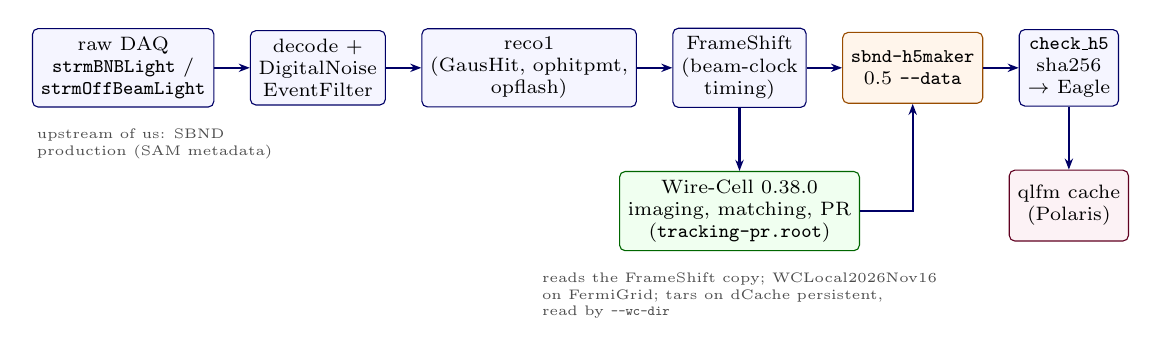
\begin{tikzpicture}[node distance=0.35cm and 0.45cm]
    \node[box] (raw) {raw DAQ\\\code{strmBNBLight} /\\\code{strmOffBeamLight}};
    \node[box, right=of raw] (dec) {decode +\\DigitalNoise\\EventFilter};
    \node[box, right=of dec] (reco) {reco1\\(GausHit, ophitpmt,\\opflash)};
    \node[box, right=of reco] (fs) {FrameShift\\(beam-clock\\timing)};
    \node[box, right=of fs, fill=orange!8, draw=orange!60!black] (h5) {\code{sbnd-h5maker}\\0.5 \code{--data}};
    \node[box, below=0.8cm of fs, fill=green!6, draw=green!40!black] (wc) {Wire-Cell 0.38.0\\imaging, matching, PR\\(\code{tracking-pr.root})};
    \node[box, right=of h5] (chk) {\code{check\_h5}\\sha256\\$\to$ Eagle};
    \node[box, below=0.8cm of chk, fill=purple!5, draw=purple!50!black] (q) {qlfm cache\\(Polaris)};
    \draw[arr] (raw) -- (dec); \draw[arr] (dec) -- (reco); \draw[arr] (reco) -- (fs); \draw[arr] (fs) -- (h5);
    \draw[arr] (h5) -- (chk); \draw[arr] (chk) -- (q);
    \draw[arr] (fs.south) -- (wc.north); \draw[arr] (wc.east) -| (h5.south);
    \node[note, below=0.15cm of wc] {reads the FrameShift copy; WCLocal2026Nov16\\on FermiGrid; tars on dCache persistent,\\read by \code{--wc-dir}};
    \node[note, below=0.15cm of raw, xshift=0.4cm] {upstream of us: SBND\\production (SAM metadata)};
  \end{tikzpicture}\\[8pt]
  \raggedright\scriptsize
  \begin{itemize}\setlength{\itemsep}{2pt}
    \item \textbf{Per reco1 file} (``pair'') on FermiGrid: copy, FrameShift, untar the Wire-Cell output, run \code{sbnd\_h5maker.py --data},
      run \code{check\_h5.py}. 288 jobs of 10 pairs, about 1.5 h elapsed (cluster 30819860).
    \item \textbf{FrameShift} supplies \code{frame\_apply\_at\_caf\_ns} (0.25--2.8\,$\mu$s): light times move from the trigger
      clock to the beam clock, $t_\mathrm{beam} = t_\mathrm{peak} + \code{frame\_apply\_at\_caf\_ns}/1000$, as Wire-Cell does.
    \item The simulation went through the same \code{sbnd-h5maker} (0.4) and the same Wire-Cell 0.38.0 step (rebuilt 21 Nov).
  \end{itemize}
\end{frame}

\begin{frame}{What one HDF5 file holds (same layout as the simulation)}
  \footnotesize
  \centering
  \fitw{\begin{tabular}{lp{7.3cm}p{4.6cm}}
    \toprule
    table & content (one row per \dots) & data vs simulation \\
    \midrule
    \code{event\_table} & event: run/subrun/event, beam gate, time, FrameShift timing, Wire-Cell status and bundle census
      (\code{wc\_n\_bundle}, \code{wc\_n\_bundle\_cosmic}) & data: truth columns at defaults ($\nu$ PDG 0, vertex $-9999$) \\
    \code{hit\_table} & GausHit: channel, TPC, plane, wire, peak time, RMS, integral, amplitude & same producer label (\code{gaushit}) \\
    \code{ophit\_table} & PMT optical hit (\code{ophitpmt}): channel, peak time, width, area, PE; window $-10\dots40\,\mu$s & times on the trigger clock in the file \\
    \code{opflash\_table}, \code{opflashsumpe\_table} & flashes (\code{opflashtpc0/1}) and their per-PMT PE & -- \\
    \code{wc\_event\_table} & Wire-Cell $\nu$ candidate: cluster, flash time / PE / TPC, reco vertex and energy, $\nu_\mu$/$\nu_e$ scores,
      containment, \code{cosmict\_flag} & \code{cosmict\_flag} new in 0.5 \\
    \code{wc\_hit\_table} & per hit (same order as \code{hit\_table}): Wire-Cell cluster id, $\nu$-candidate index, main cluster & the label \\
    \code{nu\_table}, \code{edep\_table}, \code{particle\_table} & truth: neutrinos, Geant4 deposits projected onto hits, particles & \textbf{empty in data} \\
    \bottomrule
  \end{tabular}}\\[6pt]
  \raggedright\scriptsize
  File attributes record the detector, units, the producer labels, the Wire-Cell channel and tick conventions, and the label
  definition (\code{wc\_label\_notes}). Data: \code{is\_data} = 1, no \code{sim\_config}.
\end{frame}

\begin{frame}{Hits and light: same producers, different upstream chains}
  \footnotesize
  \begin{columns}[T]
    \begin{column}{0.58\textwidth}
      \centering
      \scriptsize
      \fitw{\begin{tabular}{lll}
        \toprule
        & simulation & real data \\
        \midrule
        reco1 release & sbndcode v10\_14\_02\_03 & production MCP2025C (v10\_14\_02) \\
        waveforms into GausHit & Wire-Cell 2D sim + noise filter + SP & noise filter + SP on real waveforms \\
        field response & \code{garfield-sbnd-v1} & the detector \\
        noise & spectra scaled from ProtoDUNE-SP & the detector \\
        hit finder & \code{gaushit} (\code{sbnd\_gaushitfinder}) & \code{gaushit} \\
        light & semi-analytic photon sim, \code{opdaq} & 120 PMTs \\
        diffusion ($D_L$, $D_T$) & 4.0, 8.8 cm$^2$/s & -- \\
        \bottomrule
      \end{tabular}}
    \end{column}
    \begin{column}{0.40\textwidth}
      \begin{itemize}\setlength{\itemsep}{3pt}
        \item The HDF5 records only the producer label for data. That the data GausHit settings equal the simulation's is
          \textbf{not verified} (the FHiCL of one data reco1 file would settle it).
        \item Geometry: 2 TPCs (drift $\pm$200\,cm), 3 planes each (U, V induction; Y collection), 0.3\,cm pitch, 0.5\,$\mu$s ticks.
        \item qlfm mirrors TPC 1 onto one drift axis and keys tokens on the TPC; light enters as 120 PMT tokens, 16 time bins.
      \end{itemize}
    \end{column}
  \end{columns}
\end{frame}

\begin{frame}{What qlfm reads (converted cache on Polaris)}
  \footnotesize
  \begin{columns}[T]
    \begin{column}{0.52\textwidth}
      \begin{itemize}\setlength{\itemsep}{3pt}
        \item \textbf{Inputs:} per hit plane, wire, drift tick, TPC, integral, RMS; per optical hit PMT, time (beam clock), PE.
        \item \textbf{Labels / references} (never model input):
          \begin{itemize}
            \item \code{hit\_pnd\_nu}: Wire-Cell $\nu$-candidate footprint;
            \item \code{hit\_pnd\_nu\_ct0}: the same, candidates passing the PR cosmic tagger;
            \item per event: brightest flash time and PE, run/subrun/event.
          \end{itemize}
        \item \textbf{Conversion:} \code{QLFM\_DETECTOR=sbnd}, 2,875 files in 2 min on one node, exit 0 for all; merged into
          61 + 36 shards; first and last shard checked column by column against their sources.
      \end{itemize}
    \end{column}
    \begin{column}{0.46\textwidth}
      \centering
      \scriptsize
      \begin{tabular}{lrr}
        \toprule
        & beam-on & off-beam \\
        \midrule
        events & 89,946 & 49,970 \\
        hits & 1,160.6M & 664.8M \\
        optical hits & 181.0M & 105.4M \\
        hits / event & 12.9k & 13.3k \\
        shards & 61 & 36 \\
        \bottomrule
      \end{tabular}\\[4pt]
      {\tiny Cache: \code{\$QLFM\_WORK/cache/sbnd\_data\_m/}. Simulation cache: \code{cache/sbnd\_m/} (12.4k hits / event).}
    \end{column}
  \end{columns}
\end{frame}

\begin{frame}{How qlfm tokenizes SBND light}
  \centering
  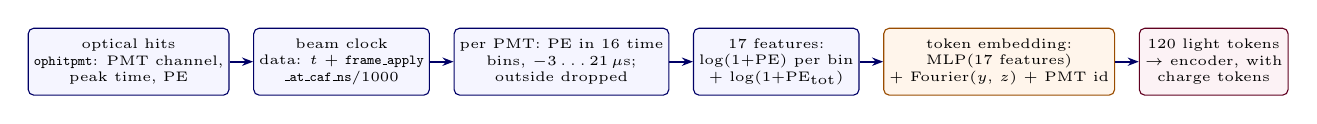
\begin{tikzpicture}[node distance=0.22cm and 0.3cm,
      sm/.style={draw=blue!40!black, rounded corners=2pt, fill=blue!4, align=center, font=\tiny, inner sep=2pt, minimum height=0.85cm}]
    \node[sm] (a) {optical hits\\\code{ophitpmt}: PMT channel,\\peak time, PE};
    \node[sm, right=of a] (b) {beam clock\\data: $t$ + \code{frame\_apply}\\\code{\_at\_caf\_ns}/1000};
    \node[sm, right=of b] (c) {per PMT: PE in 16 time\\bins, $-3\ldots21\,\mu$s;\\outside dropped};
    \node[sm, right=of c] (d) {17 features:\\$\log(1{+}\mathrm{PE})$ per bin\\+ $\log(1{+}\mathrm{PE_{tot}})$};
    \node[sm, right=of d, fill=orange!8, draw=orange!60!black] (e) {token embedding:\\MLP(17 features)\\+ Fourier($y$, $z$) + PMT id};
    \node[sm, right=of e, fill=purple!5, draw=purple!50!black] (f) {120 light tokens\\$\to$ encoder, with\\charge tokens};
    \draw[arr] (a) -- (b); \draw[arr] (b) -- (c); \draw[arr] (c) -- (d); \draw[arr] (d) -- (e); \draw[arr] (e) -- (f);
  \end{tikzpicture}\\[3pt]
  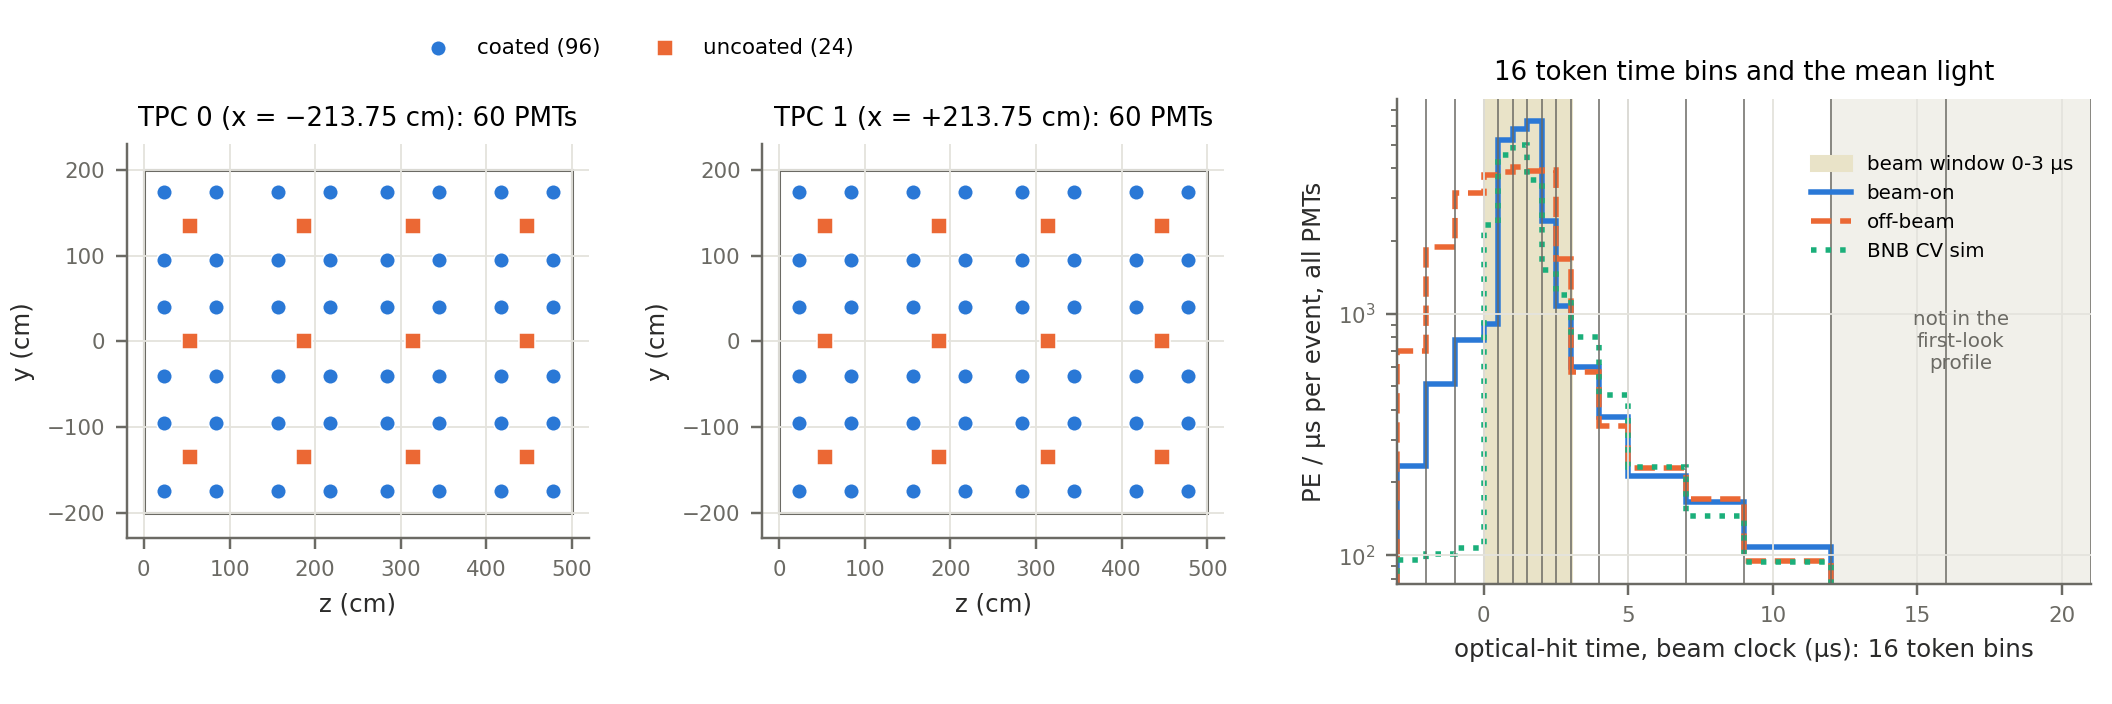
\includegraphics[width=0.88\linewidth]{figs/light_tokens.png}\\[-2pt]
  \raggedright\scriptsize
  \begin{columns}[T]
    \begin{column}{0.5\textwidth}
      \begin{itemize}\setlength{\itemsep}{1pt}
        \item \textbf{One token per PMT}: 120 PMTs (96 coated, 24 uncoated), sorted by OpChannel 6--305; the 192 X-ARAPUCAs are not used.
        \item Bins = MicroBooNE's shifted by $-3\,\mu$s: 0.5\,$\mu$s bins over the 0--3\,$\mu$s beam window, wider bins after.
        \item The T5 target (light from charge) is the same 17 features per PMT.
      \end{itemize}
    \end{column}
    \begin{column}{0.48\textwidth}
      \begin{itemize}\setlength{\itemsep}{1pt}
        \item \textbf{No $x$ in the position embedding}: facing PMTs of TPC 0 and TPC 1 share ($y$, $z$); only the learned PMT-id
          embedding tells the sides apart.
        \item The Fourier length scales (130, 1100\,cm) were set for MicroBooNE, not retuned for SBND's $\approx$400\,$\times$\,500\,cm PMT plane.
        \item Both are candidates for the light part of the simulation-to-data gap; neither is a bug.
      \end{itemize}
    \end{column}
  \end{columns}
\end{frame}

%=====================================================================
\section{How Wire-Cell labels}
\begin{frame}{Wire-Cell: from charge and light to a $\nu$ candidate}
  \centering
  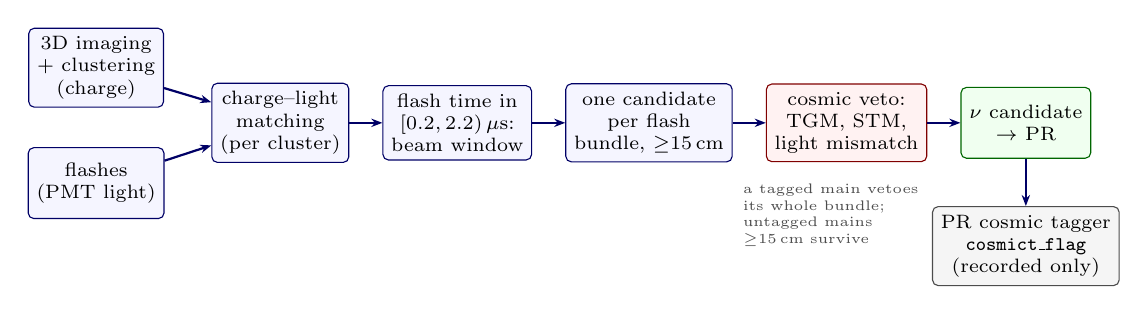
\begin{tikzpicture}[node distance=0.3cm and 0.42cm]
    \node[box] (img) {3D imaging\\+ clustering\\(charge)};
    \node[box, below=0.5cm of img] (fl) {flashes\\(PMT light)};
    \node[box, right=0.6cm of img, yshift=-0.7cm] (m) {charge--light\\matching\\(per cluster)};
    \node[box, right=of m] (bw) {flash time in\\$[0.2, 2.2)\,\mu$s:\\beam window};
    \node[box, right=of bw] (b) {one candidate\\per flash\\bundle, $\ge$15\,cm};
    \node[box, right=of b, fill=red!5, draw=red!50!black] (veto) {cosmic veto:\\TGM, STM,\\light mismatch};
    \node[box, right=of veto, fill=green!6, draw=green!40!black] (nu) {$\nu$ candidate\\$\to$ PR};
    \node[box, below=0.6cm of nu, fill=gray!8, draw=gray!60!black] (ct) {PR cosmic tagger\\\code{cosmict\_flag}\\(recorded only)};
    \draw[arr] (img) -- (m); \draw[arr] (fl) -- (m); \draw[arr] (m) -- (bw); \draw[arr] (bw) -- (b); \draw[arr] (b) -- (veto);
    \draw[arr] (veto) -- (nu); \draw[arr] (nu) -- (ct);
    \node[note, below=0.15cm of veto, xshift=-0.2cm] {a tagged main vetoes\\its whole bundle;\\untagged mains\\$\ge$15\,cm survive};
  \end{tikzpicture}\\[8pt]
  \raggedright\scriptsize
  \begin{itemize}\setlength{\itemsep}{2pt}
    \item Code: \code{clus.jsonnet}, \code{TaggerCheckNeutrino} (\code{nu\_per\_bundle}, \code{nu\_skip\_cosmic}, \code{nu\_skip\_cosmic\_bundle}).
      The same in the earlier aurora-r2 and in 0.38.0.
    \item TGM = through-going muon, STM = stopping muon; ``light mismatch'' = the cluster's predicted light disagrees with the matched flash.
    \item The PR-level cosmic tagger (OR of ten tests, plus a BDT score) and the $\nu_\mu$/$\nu_e$ scores are stored per candidate,
      \textbf{not applied} to the label. Note: \code{cosmic\_flag} is a BDT input, not the verdict.
  \end{itemize}
\end{frame}

\begin{frame}{From a candidate to a per-hit label}
  \footnotesize
  \begin{columns}[T]
    \begin{column}{0.54\textwidth}
      \begin{enumerate}\setlength{\itemsep}{4pt}
        \item \textbf{Footprint:} for every cluster of every candidate, Wire-Cell's 2D projection (\code{T\_proj\_data}): a list of
          (channel, 4-tick time slice) cells.
        \item \textbf{Match each GausHit} to a cell by channel and slice $\lfloor(t_\mathrm{peak} + 0)/4\rfloor$.
          Channels are first mapped to Wire-Cell's numbering:
          \begin{itemize}
            \item Wire-Cell: plane-major, [U0 U1][V0 V1][Y0 Y1];
            \item LArSoft: TPC-major, [U0 V0 Y0][U1 V1 Y1];
            \item offsets $(0, +1984, +3968)$ for TPC 0, $(-3654, -1670, 0)$ for TPC 1.
          \end{itemize}
        \item \textbf{Labels:} \code{wc} = hit on any candidate's footprint; \code{wc0} = only candidates with \code{cosmict\_flag} = 0.
        \item \textbf{Event label:} Wire-Cell ``selects'' an event if any hit carries the label.
      \end{enumerate}
    \end{column}
    \begin{column}{0.44\textwidth}
      \begin{itemize}\setlength{\itemsep}{4pt}
        \item \textbf{Checks that guard the matching:}
          \begin{itemize}
            \item the tick-offset scan peaks at 0 in data and simulation;
            \item \code{check\_h5}: footprint charge fraction per (TPC, plane) must be flat (applied with $\ge$10 candidate events).
          \end{itemize}
        \item \textbf{Why the check exists:} in the first SBND files (\iss{11}) the channel numbering was not remapped. Labels
          matched only one plane per TPC (efficiency $\approx$0 on four of six planes). Fixed in \code{sbnd-h5maker} 0.4.
        \item \textbf{MicroBooNE differs} (\iss{10}): label = in-time \emph{main} cluster \emph{and} the generic-$\nu$
          event selection (cosmic taggers applied): efficiency 0.53, purity 0.95.
      \end{itemize}
    \end{column}
  \end{columns}
\end{frame}

\begin{frame}{\code{cosmict\_flag}: what it is and at which level it acts}
  \centering
  \fitw{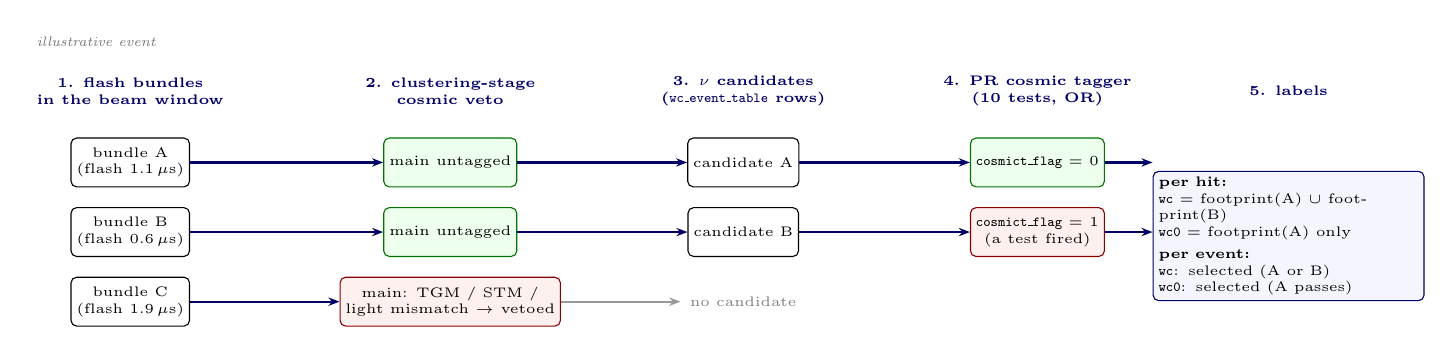
\begin{tikzpicture}[node distance=0.25cm and 0.35cm,
      sm/.style={draw, rounded corners=2pt, align=center, font=\tiny, inner sep=2pt, minimum height=0.62cm},
      ok/.style={sm, fill=green!7, draw=green!45!black}, ko/.style={sm, fill=red!6, draw=red!55!black},
      st/.style={font=\tiny\bfseries, text=blue!40!black, align=center}]
    % stage labels
    \node[st] (s1) at (0, 0) {1. flash bundles\\in the beam window};
    \node[font=\tiny\itshape, text=black!55, anchor=south west] at ([yshift=0.15cm]s1.north west) {illustrative event};
    \node[st, right=1.55cm of s1] (s2) {2. clustering-stage\\cosmic veto};
    \node[st, right=1.35cm of s2] (s3) {3. $\nu$ candidates\\(\code{wc\_event\_table} rows)};
    \node[st, right=1.25cm of s3] (s4) {4. PR cosmic tagger\\(10 tests, OR)};
    \node[st, right=1.25cm of s4] (s5) {5. labels};
    % bundle A
    \node[sm, below=0.3cm of s1] (bA) {bundle A\\(flash 1.1\,$\mu$s)};
    \node[sm, below=of bA] (bB) {bundle B\\(flash 0.6\,$\mu$s)};
    \node[sm, below=of bB] (bC) {bundle C\\(flash 1.9\,$\mu$s)};
    \node[ok] (vA) at (bA -| s2) {main untagged};
    \node[ok] (vB) at (bB -| s2) {main untagged};
    \node[ko] (vC) at (bC -| s2) {main: TGM / STM /\\light mismatch $\to$ vetoed};
    \node[sm] (cA) at (bA -| s3) {candidate A};
    \node[sm] (cB) at (bB -| s3) {candidate B};
    \node[font=\tiny, text=black!50] (cC) at (bC -| s3) {no candidate};
    \node[ok] (tA) at (bA -| s4) {\code{cosmict\_flag} = 0};
    \node[ko] (tB) at (bB -| s4) {\code{cosmict\_flag} = 1\\(a test fired)};
    \draw[arr] (bA) -- (vA); \draw[arr] (bB) -- (vB); \draw[arr] (bC) -- (vC);
    \draw[arr] (vA) -- (cA); \draw[arr] (vB) -- (cB); \draw[arr, black!40] (vC) -- (cC);
    \draw[arr] (cA) -- (tA); \draw[arr] (cB) -- (tB);
    \node[sm, fill=blue!4, draw=blue!40!black, text width=3.3cm, align=left] (lab) at ([yshift=-0.05cm]bB -| s5) {
      \textbf{per hit:}\\
      \code{wc} = footprint(A) $\cup$ footprint(B)\\
      \code{wc0} = footprint(A) only\\[2pt]
      \textbf{per event:}\\
      \code{wc}: selected (A or B)\\
      \code{wc0}: selected (A passes)};
    \draw[arr] (tA.east) -- (lab.west |- tA.east); \draw[arr] (tB.east) -- (lab.west |- tB.east);
  \end{tikzpicture}}\\[8pt]
  \raggedright\scriptsize
  \begin{columns}[T]
    \begin{column}{0.50\textwidth}
      \begin{itemize}\setlength{\itemsep}{2pt}
        \item \textbf{Level: per $\nu$ candidate}, one value per \code{wc\_event\_table} row; an event can hold several candidates.
          Neither per hit nor per event in the files; our \code{hit\_pnd\_nu\_ct0} and event \code{wc0} are derived from it.
        \item \textbf{Verdict = OR of the tagger's ten tests} on the candidate's 3D PR topology, with a BDT score \code{cosmict\_score}.
          \code{cosmic\_flag} is only one BDT input (flag 9), not the verdict.
      \end{itemize}
    \end{column}
    \begin{column}{0.48\textwidth}
      \begin{itemize}\setlength{\itemsep}{2pt}
        \item \textbf{It does not contain the TGM / STM / light-mismatch taggers:} those act earlier (stage 2) and remove bundles before
          any candidate exists, so every candidate, and the plain \code{wc} label, has already passed them. \code{cosmict\_flag} is a
          second, later test.
        \item Effect on data: keeps 88\% of labelled beam-on charge, 49\% of off-beam charge. The ten tests are not listed here
          (WCT source not checked from Polaris).
      \end{itemize}
    \end{column}
  \end{columns}
\end{frame}

\begin{frame}{How good is the label, and how often does it fire?}
  \footnotesize
  \begin{columns}[T]
    \begin{column}{0.50\textwidth}
      \centering
      \scriptsize
      \textbf{Against truth on the simulation test split}\\(10k events with a visible in-AV $\nu$, charge-weighted)\\[3pt]
      \begin{tabular}{lccc}
        \toprule
        & efficiency & purity & F1 \\
        \midrule
        Wire-Cell \code{wc} & 0.917 & 0.946 & \textbf{0.931} \\
        Wire-Cell \code{wc0} & 0.892 & 0.947 & 0.919 \\
        qlfm SBND-pre CL (1\% labels) & 0.922 & 0.922 & 0.922 \\
        \bottomrule
      \end{tabular}
    \end{column}
    \begin{column}{0.48\textwidth}
      \centering
      \scriptsize
      \textbf{On real data} (all events)\\[3pt]
      \begin{tabular}{lcc}
        \toprule
        & beam-on & off-beam \\
        \midrule
        $\nu$ candidates & 42,328 & 4,741 \\
        events selected, \code{wc} & 44.9\% & 5.8\% \\
        events selected, \code{wc0} & 38.6\% & 3.2\% \\
        share of all charge, \code{wc} & 3.8\% & 0.49\% \\
        share of all charge, \code{wc0} & 3.3\% & 0.24\% \\
        \bottomrule
      \end{tabular}
    \end{column}
  \end{columns}
  \vspace{8pt}
  \begin{itemize}\setlength{\itemsep}{3pt}
    \item On simulation the label is high quality; qlfm at 1\% labels is close to it.
    \item On data the cosmic tagger keeps 88\% of the labelled beam-on charge but only 49\% of the off-beam charge: it removes
      mostly cosmic candidates, as intended.
    \item Beam-on minus off-beam, about 39 points of selected events, is the beam-related excess the models are compared against.
      Wire-Cell is a \textbf{reference, not truth}, on data.
  \end{itemize}
\end{frame}

%=====================================================================
\section{Experiments}
\begin{frame}{Experiments done}
  \footnotesize
  \centering
  \fitw{\begin{tabular}{llp{6.8cm}l}
    \toprule
    id & experiment & what it measures & status \\
    \midrule
    E1 & 10k simulation pipeline test (\iss{11}) & conversion, training, MicroBooNE-to-SBND transfer & done \\
    E2 & full simulation: pretraining + 13 fine-tunes (\iss{11}) & SBND-pretrained vs MicroBooNE-pretrained vs no pretraining, T1--T5 & done \\
    \textbf{E3} & \textbf{first look at real data} (\iss{14}) & data vs simulation: hit width per plane and drift, hit charge, light timing, Wire-Cell rates & \textbf{done} \\
    \textbf{E4} & \textbf{13 models vs Wire-Cell on real data} (\iss{14}) & sim-trained models on beam-on / off-beam; event and hit agreement with Wire-Cell & \textbf{done} \\
    \textbf{E5} & \textbf{width test} (\iss{14}) & the same 13 models on simulation with data-like hit widths (V$\times$0.97, Y$\times$0.955): how much of the data drop does width explain? & \textbf{done} \\
    \textbf{E6} & \textbf{data-like-width fine-tune} (\iss{14}) & CL and C+XF fine-tuned on simulation with data-like widths (3 seeds each), then E4 again & \textbf{done} \\
    \textbf{E7} & \textbf{real-data fine-tune with Wire-Cell labels} (\iss{14}) & CL and C+XF continued from E2 on real data, Wire-Cell labels (3 seeds each); held-out files & \textbf{done} \\
    \textbf{D} & \textbf{event displays} & 20 random events each from simulation, beam-on, off-beam; hit and light predictions of 3 models & \textbf{done} \\
    \bottomrule
  \end{tabular}}\\[8pt]
  \raggedright\scriptsize
  \begin{itemize}\setlength{\itemsep}{2pt}
    \item E7 is the only experiment that trains on real data; E2--E6 models see simulation only.
    \item Scripts: \code{scripts/sbnd\_data\_firstlook.py} (E3), \code{qlfm/eval\_sbnd\_data.py} (E4--E7), \code{scripts/refresh\_wc\_labels.py} (the \code{wc0} label),
      \code{scripts/sbnd\_event\_displays.py} (D), \code{scripts/plot\_sbnd\_realdata\_campaign.py} (figures).
  \end{itemize}
\end{frame}

\begin{frame}{E3: data vs simulation at a glance}
  \footnotesize
  \centering
  \scriptsize
  20k random events per sample; all hits (mostly cosmics) and all optical hits\\[3pt]
  \fitw{\begin{tabular}{lccc}
    \toprule
    & beam-on & off-beam & BNB CV simulation \\
    \midrule
    hits per event & 12.9k & 13.3k & 12.4k \\
    median hit RMS, U / V / Y (ticks) & 3.52 / 3.40 / 3.35 & 3.52 / 3.40 / 3.36 & 3.50 / 3.50 / 3.51 \\
    Y-plane hit integral, 10 / 50 / 90\% & \bad{183} / 612 / 1,597 & \bad{175} / 632 / 1,634 & 304 / 609 / 1,585 \\
    brightest flash time, 10 / 50 / 90\% ($\mu$s, beam clock) & 0.53 / 1.28 / 2.03 & $-$1.00 / 0.79 / 2.38 & 0.30 / 0.99 / 1.70 \\
    brightest flash in the 0--3\,$\mu$s window & 88\% & \bad{65\%} & 88\% \\
    brightest-flash PE, median & 9.4k & 14.1k & 7.3k \\
    events with a Wire-Cell candidate & 45.3\% & 5.7\% & 46.1\% \\
    \bottomrule
  \end{tabular}}\\[6pt]
  \raggedright
  \begin{itemize}\setlength{\itemsep}{2pt}
    \item \textbf{More low-charge Y hits in data} (10th percentile 175--183 vs 304) with the same median: the hit threshold or noise differs.
    \item The two data samples agree with each other on hit width and charge: these are detector effects, not event-mix effects.
    \item The beam-on and simulation Wire-Cell rates agree by coincidence (trigger selection vs a $\nu$ in every simulated event).
  \end{itemize}
\end{frame}

\begin{frame}{E3: hit width, data / simulation}
  \begin{columns}[T]
    \begin{column}{0.56\textwidth}
      \centering
      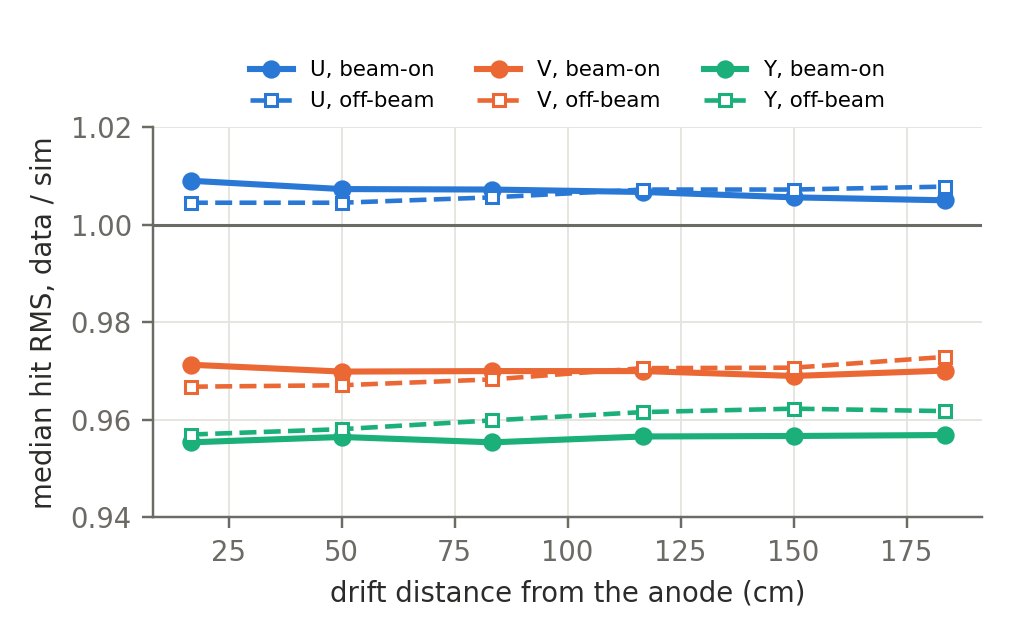
\includegraphics[width=\linewidth]{figs/width_ratio.png}
    \end{column}
    \begin{column}{0.42\textwidth}
      \footnotesize
      \begin{itemize}\setlength{\itemsep}{4pt}
        \item Median hit RMS in six drift bins, all hits.
        \item \textbf{U matches; V is 3\% and Y 4.5\% narrower in data}, the same in beam-on and off-beam.
        \item \textbf{Flat in drift.} On MicroBooNE the data/sim factor falls with drift (a diffusion mismatch, Sunny's
          measurement, \iss{9}). A constant per-plane offset points to the field response or the shaping, not diffusion.
        \item Caveat: medians over all hits, not a track-matched measurement like \iss{9}.
        \item Width was qlfm's main data/simulation cue on MicroBooNE.
      \end{itemize}
    \end{column}
  \end{columns}
\end{frame}

\begin{frame}{E3: light timing}
  \begin{columns}[T]
    \begin{column}{0.56\textwidth}
      \centering
      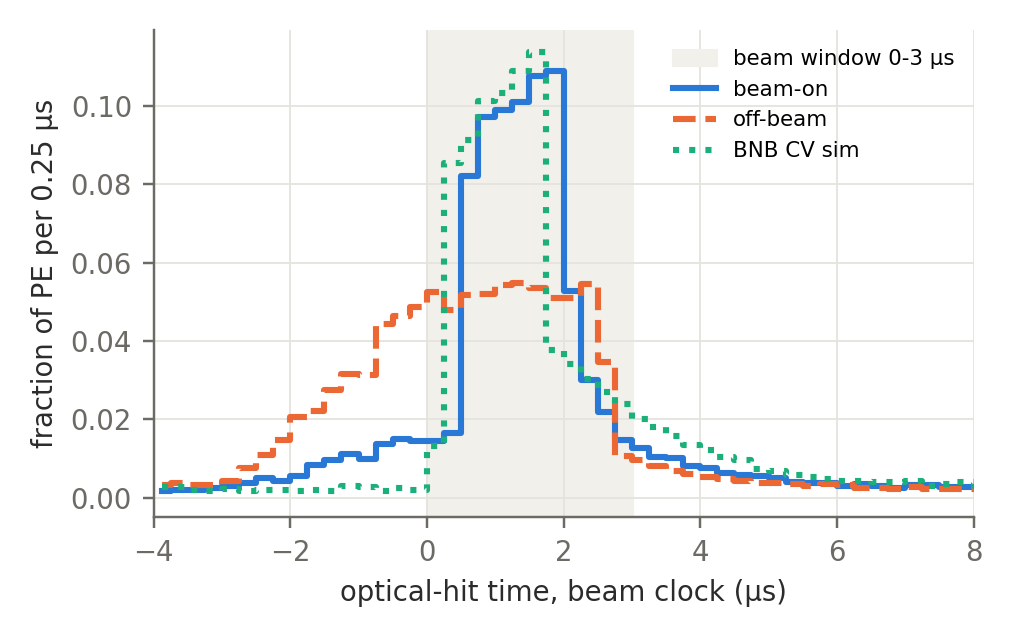
\includegraphics[width=\linewidth]{figs/light_profile.png}
    \end{column}
    \begin{column}{0.42\textwidth}
      \footnotesize
      \begin{itemize}\setlength{\itemsep}{4pt}
        \item PE-weighted optical-hit time on the beam clock, normalised per sample.
        \item \textbf{Beam-on light is $\approx$0.3\,$\mu$s later than simulation} (brightest-flash median 1.28 vs 0.99\,$\mu$s).
          Small against the 3\,$\mu$s window, but a model can read it.
        \item \textbf{Off-beam light is spread over $-3\ldots3\,\mu$s}: a different trigger window. A third of off-beam events have
          their brightest flash outside the beam window.
        \item Flash time alone separates beam-on from off-beam with AUC 0.62. When off-beam serves as ``no $\nu$'', compare
          methods at a \textbf{fixed off-beam rate}, and check events with a beam-window flash separately.
      \end{itemize}
    \end{column}
  \end{columns}
\end{frame}

\begin{frame}{E4 setup: models and metrics}
  \footnotesize
  \begin{columns}[T]
    \begin{column}{0.54\textwidth}
      \centering
      \scriptsize
      \textbf{The 13 models} (E2; multi-task, fine-tuned on the SBND simulation with 1\% labels; simulation test)\\[3pt]
      \fitw{\begin{tabular}{lcccccc}
        \toprule
        model & seeds & T1 F1 & T2 AUC & T3 F1 & T4 res & T5 MSE \\
        \midrule
        SBND-pretrained CL, fine-tuned & 3 & 0.921 & 0.996 & 0.77 & 0.22 & 0.62 \\
        SBND-pretrained C+XF & 3 & 0.896 & 0.992 & 0.73 & 0.23 & 0.78 \\
        MicroBooNE-pretrained CL & 3 & 0.903 & 0.995 & 0.74 & 0.23 & 0.74 \\
        SBND-pretrained CL, frozen & 1 & 0.876 & 0.997 & 0.72 & 0.23 & 0.59 \\
        no pretraining & 3 & 0.804 & 0.995 & 0.68 & 0.25 & 0.94 \\
        \bottomrule
      \end{tabular}}\\[3pt]
      {\tiny CL = qlfm-M with light in pretraining; C+XF = charge-only pretraining, light fused at the head.
      T1 hits, T2 $\nu$/no-$\nu$, T3 flavour, T4 energy, T5 light from charge.}
    \end{column}
    \begin{column}{0.44\textwidth}
      \begin{itemize}\setlength{\itemsep}{3pt}
        \item \textbf{Run on every event} of both samples, no retraining (0.4 node-h, debug queue).
        \item \textbf{Event level:} each model's $\nu$ log-odds cut is set so it passes the \emph{same off-beam fraction} as Wire-Cell;
          compare beam-on pass rates.
        \item \textbf{Hit level}, on beam-on events with a Wire-Cell candidate (40,404):
          \begin{itemize}
            \item share of Wire-Cell's $\nu$ charge the model also tags;
            \item share of the model's $\nu$ charge inside the Wire-Cell footprint.
          \end{itemize}
        \item \textbf{Reference:} the same hit shares on simulation test events with a visible in-AV $\nu$ and a Wire-Cell candidate (14,002).
      \end{itemize}
    \end{column}
  \end{columns}
\end{frame}

\begin{frame}{E4: event level}
  \begin{columns}[T]
    \begin{column}{0.52\textwidth}
      \centering
      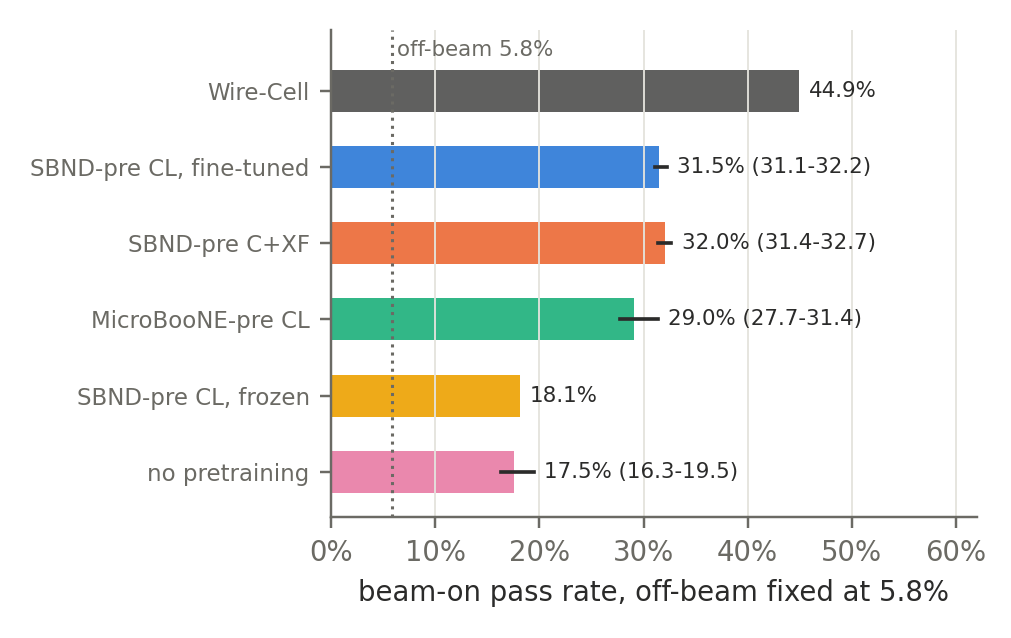
\includegraphics[width=\linewidth]{figs/event_level.png}
    \end{column}
    \begin{column}{0.46\textwidth}
      \centering
      \scriptsize
      beam-on pass rate at Wire-Cell's off-beam rate\\[3pt]
      \fitw{\begin{tabular}{lccc}
        \toprule
        & \code{wc}, all & \code{wc}, flash in window & \code{wc0} \\
        off-beam fixed at & 5.8\% & 8.4\% & 3.2\% \\
        \midrule
        \textbf{Wire-Cell} & \textbf{44.9\%} & \textbf{48.4\%} & \textbf{38.6\%} \\
        SBND-pre CL & 31.1--32.2 & 34.2--35.6 & 25.8--26.9 \\
        SBND-pre C+XF & 31.4--32.7 & 35.2--36.0 & 26.2--27.3 \\
        MicroBooNE-pre CL & 27.7--31.4 & 30.0--34.4 & 20.2--24.6 \\
        SBND-pre CL, frozen & 18.1 & 20.0 & 12.6 \\
        no pretraining & 16.3--19.5 & 18.6--22.6 & 11.1--13.5 \\
        \bottomrule
      \end{tabular}}\\[4pt]
      \raggedright\footnotesize
      \begin{itemize}\setlength{\itemsep}{2pt}
        \item SBND-pretrained fine-tuned models keep \textbf{about 2/3 of Wire-Cell's beam-on excess} over off-beam (25--27 vs 39 points); MicroBooNE-pretrained 22--26.
        \item The ordering holds with the beam-window restriction and with the cosmic-tagged label.
      \end{itemize}
    \end{column}
  \end{columns}
\end{frame}

\begin{frame}{E4: hit level}
  \begin{columns}[T]
    \begin{column}{0.56\textwidth}
      \centering
      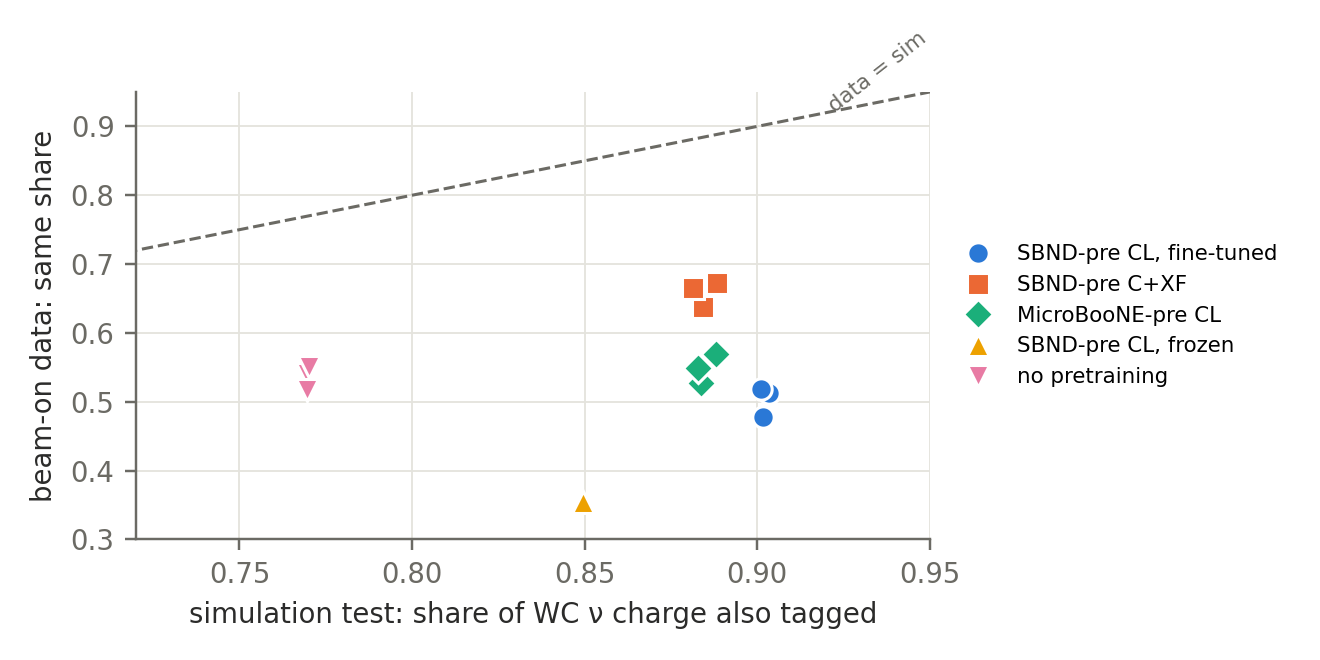
\includegraphics[width=\linewidth]{figs/agreement.png}\\[2pt]
      \scriptsize
      \fitw{\begin{tabular}{lccc}
        \toprule
        & model charge in WC footprint & \multicolumn{2}{c}{share of all charge called $\nu$} \\
        & data / sim & beam-on & off-beam \\
        \midrule
        Wire-Cell & -- & 3.8\% & 0.49\% \\
        SBND-pre CL & 0.84--0.86 / 0.90 & 2.8--3.2\% & 0.9--1.1\% \\
        SBND-pre C+XF & 0.82--0.83 / 0.88 & 4.1--4.6\% & 2.1--2.9\% \\
        MicroBooNE-pre CL & 0.80--0.82 / 0.89 & 3.4--3.8\% & 1.5--2.0\% \\
        no pretraining & 0.71--0.72 / 0.82 & 4.1--4.4\% & 3.0--3.1\% \\
        \bottomrule
      \end{tabular}}
    \end{column}
    \begin{column}{0.42\textwidth}
      \footnotesize
      \begin{itemize}\setlength{\itemsep}{4pt}
        \item \textbf{Every model falls well below the diagonal:} 0.77--0.91 of Wire-Cell's $\nu$ charge on simulation, 0.35--0.67 on beam-on.
        \item \textbf{They lose real $\nu$ hits rather than tag cosmics:} what they tag is still mostly inside Wire-Cell's footprint.
        \item \textbf{C+XF keeps the most} on data (0.64--0.67 vs 0.48--0.52 for CL), but calls more off-beam charge $\nu$.
        \item The best model on simulation (SBND-pre CL) drops the most among the fine-tuned ones; the frozen backbone drops further (0.35).
        \item The cosmic-tagged label \code{wc0} gives the same picture (shares +0.01--0.02).
      \end{itemize}
    \end{column}
  \end{columns}
\end{frame}

%=====================================================================
\begin{frame}{E5: how much of the drop is hit width?}
  \begin{columns}[T]
    \begin{column}{0.55\textwidth}
      \centering
      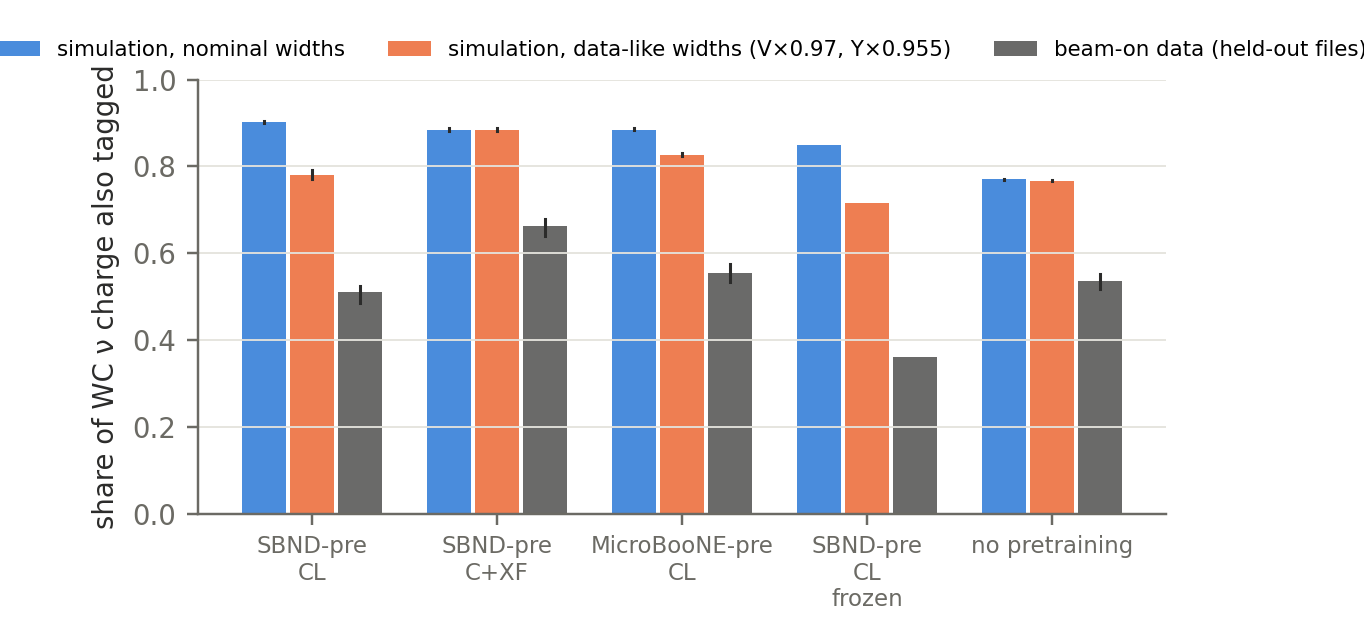
\includegraphics[width=\linewidth]{figs/width_test.png}\\[2pt]
      \scriptsize
      \fitw{\begin{tabular}{lccc}
        \toprule
        & T1 F1 vs truth, sim & \multicolumn{2}{c}{share of WC $\nu$ charge tagged} \\
        & nominal / data-like & sim nominal / data-like & data \\
        \midrule
        SBND-pre CL & 0.92 / \bad{0.85} & 0.90 / \bad{0.78} & 0.49--0.53 \\
        SBND-pre C+XF & 0.90 / 0.90 & 0.88 / 0.88 & 0.64--0.68 \\
        MicroBooNE-pre CL & 0.90 / 0.86 & 0.89 / 0.83 & 0.53--0.58 \\
        SBND-pre CL, frozen & 0.88 / 0.80 & 0.85 / 0.72 & 0.36 \\
        no pretraining & 0.80 / 0.80 & 0.77 / 0.77 & 0.52--0.55 \\
        \bottomrule
      \end{tabular}}
    \end{column}
    \begin{column}{0.43\textwidth}
      \footnotesize
      \begin{itemize}\setlength{\itemsep}{4pt}
        \item \textbf{Test:} rescale every simulated hit width to data, V$\times$0.97 and Y$\times$0.955 (the E3 ratios), and rerun the
          13 models on the simulation test events. No retraining (\code{--perturb w\_sbnd}).
        \item \textbf{CL models read width:} SBND-pre CL loses 0.07 F1 against truth and drops 0.90 $\to$ 0.78 in agreement with
          Wire-Cell, \textbf{about a third of its data drop} (0.90 $\to$ 0.51). The frozen CL drops similarly.
        \item \textbf{C+XF and no-pretraining do not move}, yet they still drop on data (C+XF 0.88 $\to$ 0.66).
        \item So width is one cause, for CL only. Another simulation-to-data difference remains: candidates are the extra
          low-charge hits (E3) and the 0.3\,$\mu$s light-timing shift.
      \end{itemize}
    \end{column}
  \end{columns}
\end{frame}

\begin{frame}{E6 and E7: two fixes, setup}
  \footnotesize
  \begin{columns}[T]
    \begin{column}{0.49\textwidth}
      \textbf{E6: fine-tune with data-like widths}
      \begin{itemize}\setlength{\itemsep}{3pt}
        \item Same recipe as E2 (SBND-pretrained encoder, 1\% labels = 7,380 simulated events, 6,000 steps, all five tasks), but every
          simulated hit width is rescaled to data during training (\code{--width sbnd}).
        \item SBND-pre CL and C+XF, 3 seeds each; about 45 min per run on one A100.
        \item At test time on real data the widths are untouched.
      \end{itemize}
    \end{column}
    \begin{column}{0.49\textwidth}
      \textbf{E7: fine-tune on real data with Wire-Cell labels}
      \begin{itemize}\setlength{\itemsep}{3pt}
        \item Continue from each E2 model on beam-on + off-beam events (\code{--labels wc\_sbnd}):
          \begin{itemize}
            \item T1 target = Wire-Cell footprint hits (\code{wc});
            \item T2 target = event has a Wire-Cell hit;
            \item T5 light from charge (measured light, no label needed).
          \end{itemize}
        \item Real data split \textbf{by source file} 75/5/20; 102,979 training events, 3,000 steps, learning rate $10^{-4}$;
          15--20 min per run.
        \item SBND-pre CL and C+XF, 3 seeds each.
      \end{itemize}
    \end{column}
  \end{columns}
  \vspace{6pt}
  \raggedright
  All data numbers for E5--E7 on the following slides are on the \textbf{held-out 20\% of files} (18,664 beam-on, 10,348 off-beam events),
  so E7 is tested on files it never saw. Wire-Cell on these files: 44.8\% of beam-on and 6.0\% of off-beam events selected.
\end{frame}

\begin{frame}{E6 and E7: results on held-out real data}
  \begin{columns}[T]
    \begin{column}{0.60\textwidth}
      \centering
      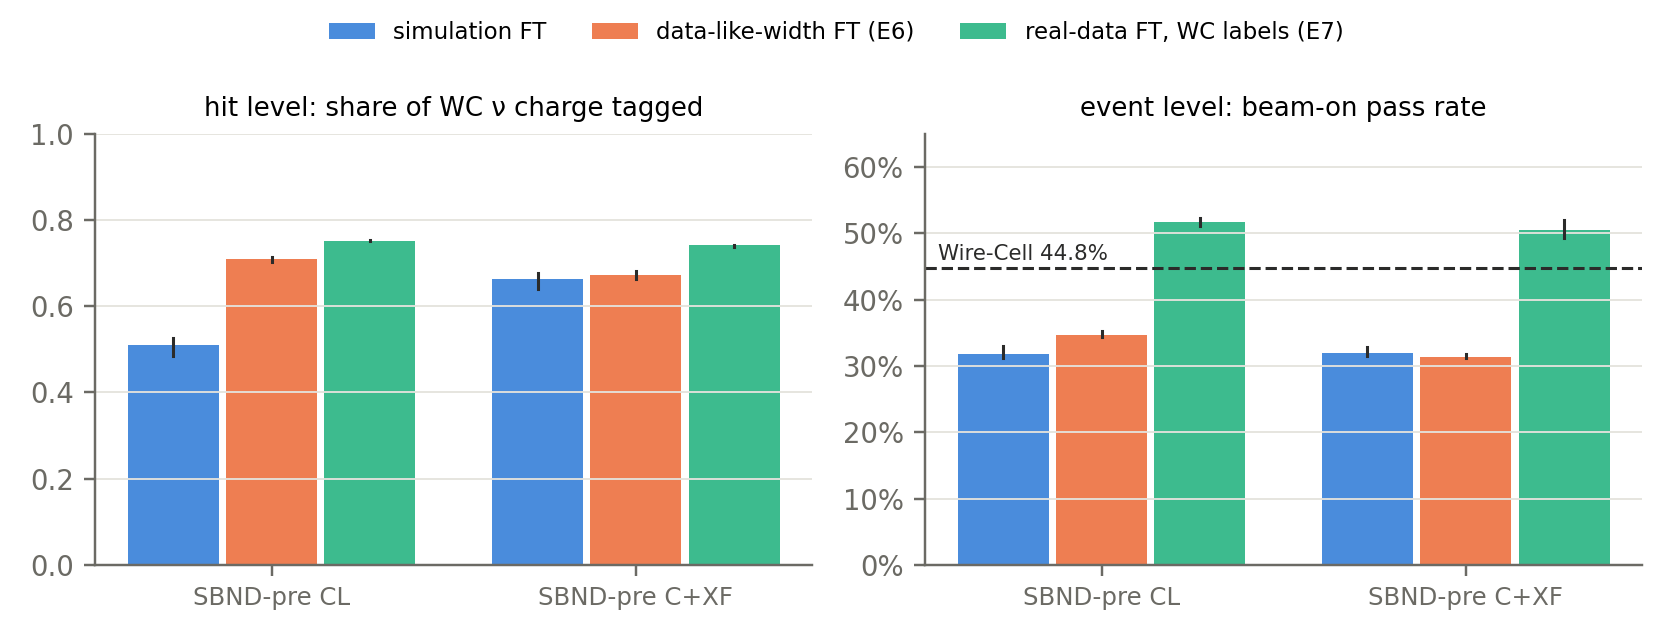
\includegraphics[width=\linewidth]{figs/fixes.png}\\[2pt]
      {\scriptsize Beam-on pass rate at Wire-Cell's off-beam rate (6.0\%); error bars span the 3 seeds. Table on the next slide.}
    \end{column}
    \begin{column}{0.38\textwidth}
      \footnotesize
      \begin{itemize}\setlength{\itemsep}{5pt}
        \item \textbf{E6 fixes much of CL's gap:} agreement with Wire-Cell 0.51 $\to$ \good{0.71}, now above C+XF. It costs 0.04 F1
          against truth on nominal-width simulation. C+XF does not move, as E5 predicts.
        \item \textbf{E7 agrees with Wire-Cell best} (0.74--0.75 of its $\nu$ charge, 0.91 inside its footprint), calls almost no
          off-beam charge $\nu$, and passes \emph{more} beam-on events than Wire-Cell at the same off-beam rate (49--52\% vs 44.8\%).
        \item \textbf{E7 is not an independent check:} it was trained to imitate Wire-Cell. Whether its extra beam-on events are
          neutrinos needs a scan.
      \end{itemize}
    \end{column}
  \end{columns}
\end{frame}

\begin{frame}{E6 and E7: numbers}
  \centering
  \scriptsize
  \fitw{\begin{tabular}{lcccccc}
    \toprule
    & \multicolumn{2}{c}{T1 F1 vs truth, simulation} & \multicolumn{2}{c}{held-out beam-on events with a WC candidate} & beam-on selected at & share of off-beam \\
    & nominal widths & data-like widths & WC $\nu$ charge tagged & model $\nu$ charge in WC & WC's off-beam rate & charge called $\nu$ \\
    \midrule
    \multicolumn{7}{l}{\textbf{SBND-pretrained CL}} \\
    simulation fine-tune (E2) & 0.92 & 0.85 & 0.49--0.53 & 0.84--0.86 & 31--33\% & 0.9--1.1\% \\
    data-like-width fine-tune (E6) & 0.88 & 0.92 & \good{0.70--0.71} & 0.86--0.87 & 34--35\% & 1.0--1.3\% \\
    real-data fine-tune, WC labels (E7) & 0.84--0.86 & 0.91 & \good{0.75} & 0.91 & \good{51--52\%} & 0.06--0.07\% \\
    \midrule
    \multicolumn{7}{l}{\textbf{SBND-pretrained C+XF}} \\
    simulation fine-tune (E2) & 0.90 & 0.90 & 0.64--0.68 & 0.82--0.83 & 32--33\% & 2.1--3.0\% \\
    data-like-width fine-tune (E6) & 0.89 & 0.89 & 0.66--0.68 & 0.80--0.82 & 31--32\% & 2.6--3.6\% \\
    real-data fine-tune, WC labels (E7) & 0.87--0.89 & 0.87--0.89 & \good{0.74} & 0.90--0.91 & \good{49--52\%} & 0.07--0.10\% \\
    \midrule
    Wire-Cell & 0.93 & -- & -- & -- & 44.8\% & 0.44\% \\
    \bottomrule
  \end{tabular}}\\[8pt]
  \raggedright\footnotesize
  \begin{itemize}\setlength{\itemsep}{3pt}
    \item Ranges span 3 seeds. Data columns: held-out 20\% of files (18,664 beam-on, 10,348 off-beam events; 8,358 beam-on events with a
      Wire-Cell candidate). Simulation columns: simulation test events, T1-eligible (14,985).
    \item E7 loses F1 against truth on nominal-width simulation (CL 0.06--0.08) and, for CL, recovers it on data-like-width simulation
      (0.91): the model has adapted to data widths.
  \end{itemize}
\end{frame}

\begin{frame}{Reading}
  \footnotesize
  \begin{enumerate}\setlength{\itemsep}{6pt}
    \item \textbf{The simulation-to-data gap seen on MicroBooNE is present on SBND.} Models trained on simulation agree with Wire-Cell at
      about 0.9 on simulation and at 0.5--0.65 on real beam-on data.
    \item \textbf{Events survive better than hits.} The SBND-pretrained fine-tuned models still select about two-thirds of Wire-Cell's
      beam-on excess at the same off-beam rate.
    \item \textbf{Pretraining matters on data too.} Fine-tuned pretrained models (SBND or MicroBooNE) beat the frozen and the
      no-pretraining models at event level by more than a factor 1.5.
    \item \textbf{Width is one cause, for CL only (E5).} Data-like widths on simulation reproduce about a third of CL's data drop and none
      of C+XF's. Training with data-like widths (E6) lifts CL from 0.51 to 0.71 on data. A second, unidentified difference remains
      for every model (C+XF 0.88 $\to$ 0.66 with no width sensitivity).
    \item \textbf{Real-data fine-tuning on Wire-Cell labels (E7) gives the closest agreement} (0.75, 0.91 inside the footprint, almost
      no off-beam $\nu$ charge), but it measures how well the model imitates Wire-Cell, not how well it finds neutrinos.
  \end{enumerate}
\end{frame}

\begin{frame}{Caveats}
  \footnotesize
  \begin{itemize}\setlength{\itemsep}{5pt}
    \item \textbf{Wire-Cell is a reference, not truth, on data.} Disagreement can be the model's or Wire-Cell's; on simulation
      Wire-Cell's label has efficiency 0.92 and purity 0.95.
    \item \textbf{No exposure normalisation.} Off-beam has no spill count here; comparisons are pass rates at a matched off-beam
      rate, not $\nu$ rates per POT.
    \item \textbf{Trigger selection.} Both data samples are light-triggered; the simulation is not. The simulation reference is on
      unselected events with a $\nu$; this does not change the size of the drop.
    \item \textbf{Off-beam light timing differs} from beam-on; handled only by the beam-window restriction.
    \item \textbf{Hit producer settings in data not verified} beyond the \code{gaushit} label.
    \item \textbf{First-look widths are medians over all hits}, mostly cosmics, not a track-matched measurement; E5 and E6 use these
      ratios.
    \item \textbf{E7 is trained on Wire-Cell's labels}: agreement with Wire-Cell on held-out files is expected to rise and is not
      evidence of better neutrino finding. Whether the extra beam-on events it selects are neutrinos needs a scan.
  \end{itemize}
\end{frame}

\begin{frame}{Next steps (proposed, not started)}
  \footnotesize
  \begin{enumerate}\setlength{\itemsep}{6pt}
    \item \textbf{Find the second cause:} perturb the simulated low-charge hits / noise and the light timing toward data, as E5 did for
      width; C+XF is the clean probe (no width sensitivity).
    \item \textbf{Combine the fixes:} data-like-width fine-tune (E6), then a short real-data fine-tune (E7).
    \item \textbf{Targeted displays} of held-out beam-on events where E7 and Wire-Cell disagree (the random sample is in this deck).
    \item \textbf{Light-trigger emulation in the simulation} (beam-window PE threshold matched to the data turn-on), so simulation
      and data rates are comparable.
    \item \textbf{Track-matched width and charge comparison} on SBND cosmics (as Sunny did for MicroBooNE), and the data GausHit
      FHiCL.
  \end{enumerate}
\end{frame}

%=====================================================================
\section{Event displays}
\begin{frame}{Event displays: how to read them}
  \footnotesize
  \begin{columns}[T]
    \begin{column}{0.52\textwidth}
      \begin{itemize}\setlength{\itemsep}{3pt}
        \item \textbf{20 random events per sample} (seed 0): simulation test events from the E5 evaluation set (BNB CV, $\nu_e$CC, NC),
          and beam-on and off-beam events from the \textbf{held-out files} of the E7 split.
        \item \textbf{Three models}, all SBND-pretrained qlfm-M CL, seed 0, one per experiment:
          \begin{itemize}
            \item \textcolor[HTML]{d23f3f}{\textbf{sim FT}}: fine-tuned on simulation (E2/E4);
            \item \textcolor[HTML]{2a78d6}{\textbf{width FT}}: fine-tuned with data-like widths (E6);
            \item \textcolor[HTML]{3b9b54}{\textbf{WC-label FT}}: fine-tuned on real data with Wire-Cell labels (E7).
          \end{itemize}
        \item Simulation is shown with its nominal widths.
      \end{itemize}
    \end{column}
    \begin{column}{0.46\textwidth}
      \textbf{Page layout} (3 rows $\times$ 5 panels)
      \begin{itemize}\setlength{\itemsep}{3pt}
        \item \textbf{Row 1:} charge (channel vs raw tick; TPC 0 U, V, Y then TPC 1 U, V, Y; colour = log$_{10}$ hit integral),
          truth $\nu$ hits (simulation only), Wire-Cell footprint, Wire-Cell after the PR cosmic tagger, event summary
          (event $p(\nu)$, hit F1 vs Wire-Cell and vs truth, predicted PE).
        \item \textbf{Row 2:} each model's per-hit $p(\nu)$ (blue cosmic, red $\nu$), the measured PMT light (120 PMTs at their
          $(z, y)$, area $\propto$ PE; TPC 0 left, TPC 1 right), and the light time profile (beam window shaded).
        \item \textbf{Row 3:} each model's light predicted from charge alone (filled; black ring = measured), and per-PMT totals.
      \end{itemize}
    \end{column}
  \end{columns}
\end{frame}

\subsection{Simulation}
% Simulation 1/20: run 2105334, subrun 51, event 10; event p(nu): sim FT 0.00, width FT 0.00, WC-label FT 0.16
\begin{frame}[plain]
  \centering\vspace*{-2pt}
  \makebox[\linewidth][c]{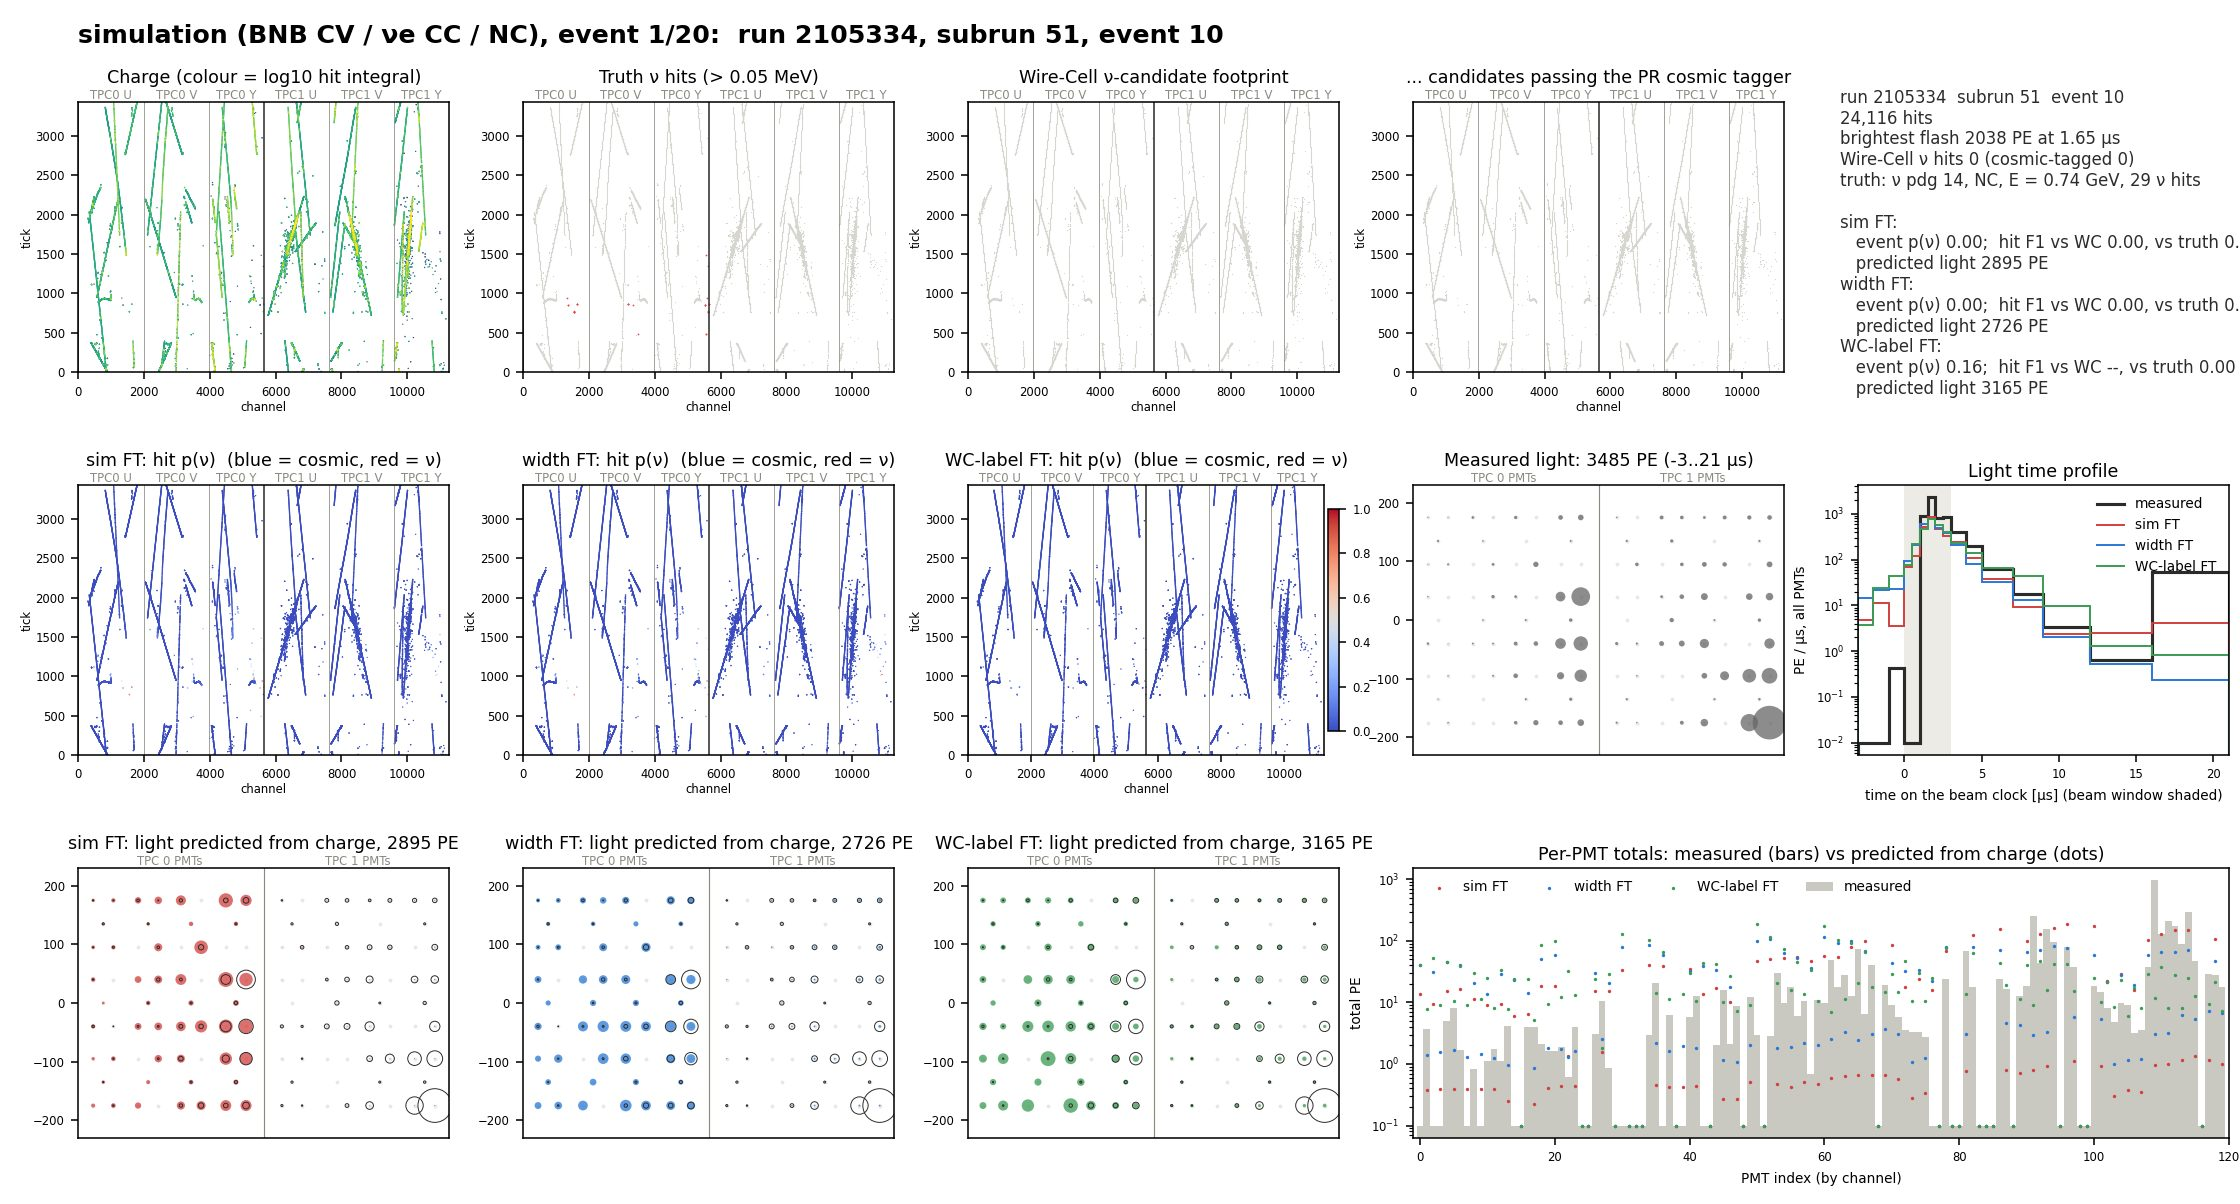
\includegraphics[width=\paperwidth,height=\paperheight,keepaspectratio]{displays/sim_00.jpg}}
\end{frame}
% Simulation 2/20: run 2110582, subrun 68, event 9; event p(nu): sim FT 0.00, width FT 0.00, WC-label FT 0.27
\begin{frame}[plain]
  \centering\vspace*{-2pt}
  \makebox[\linewidth][c]{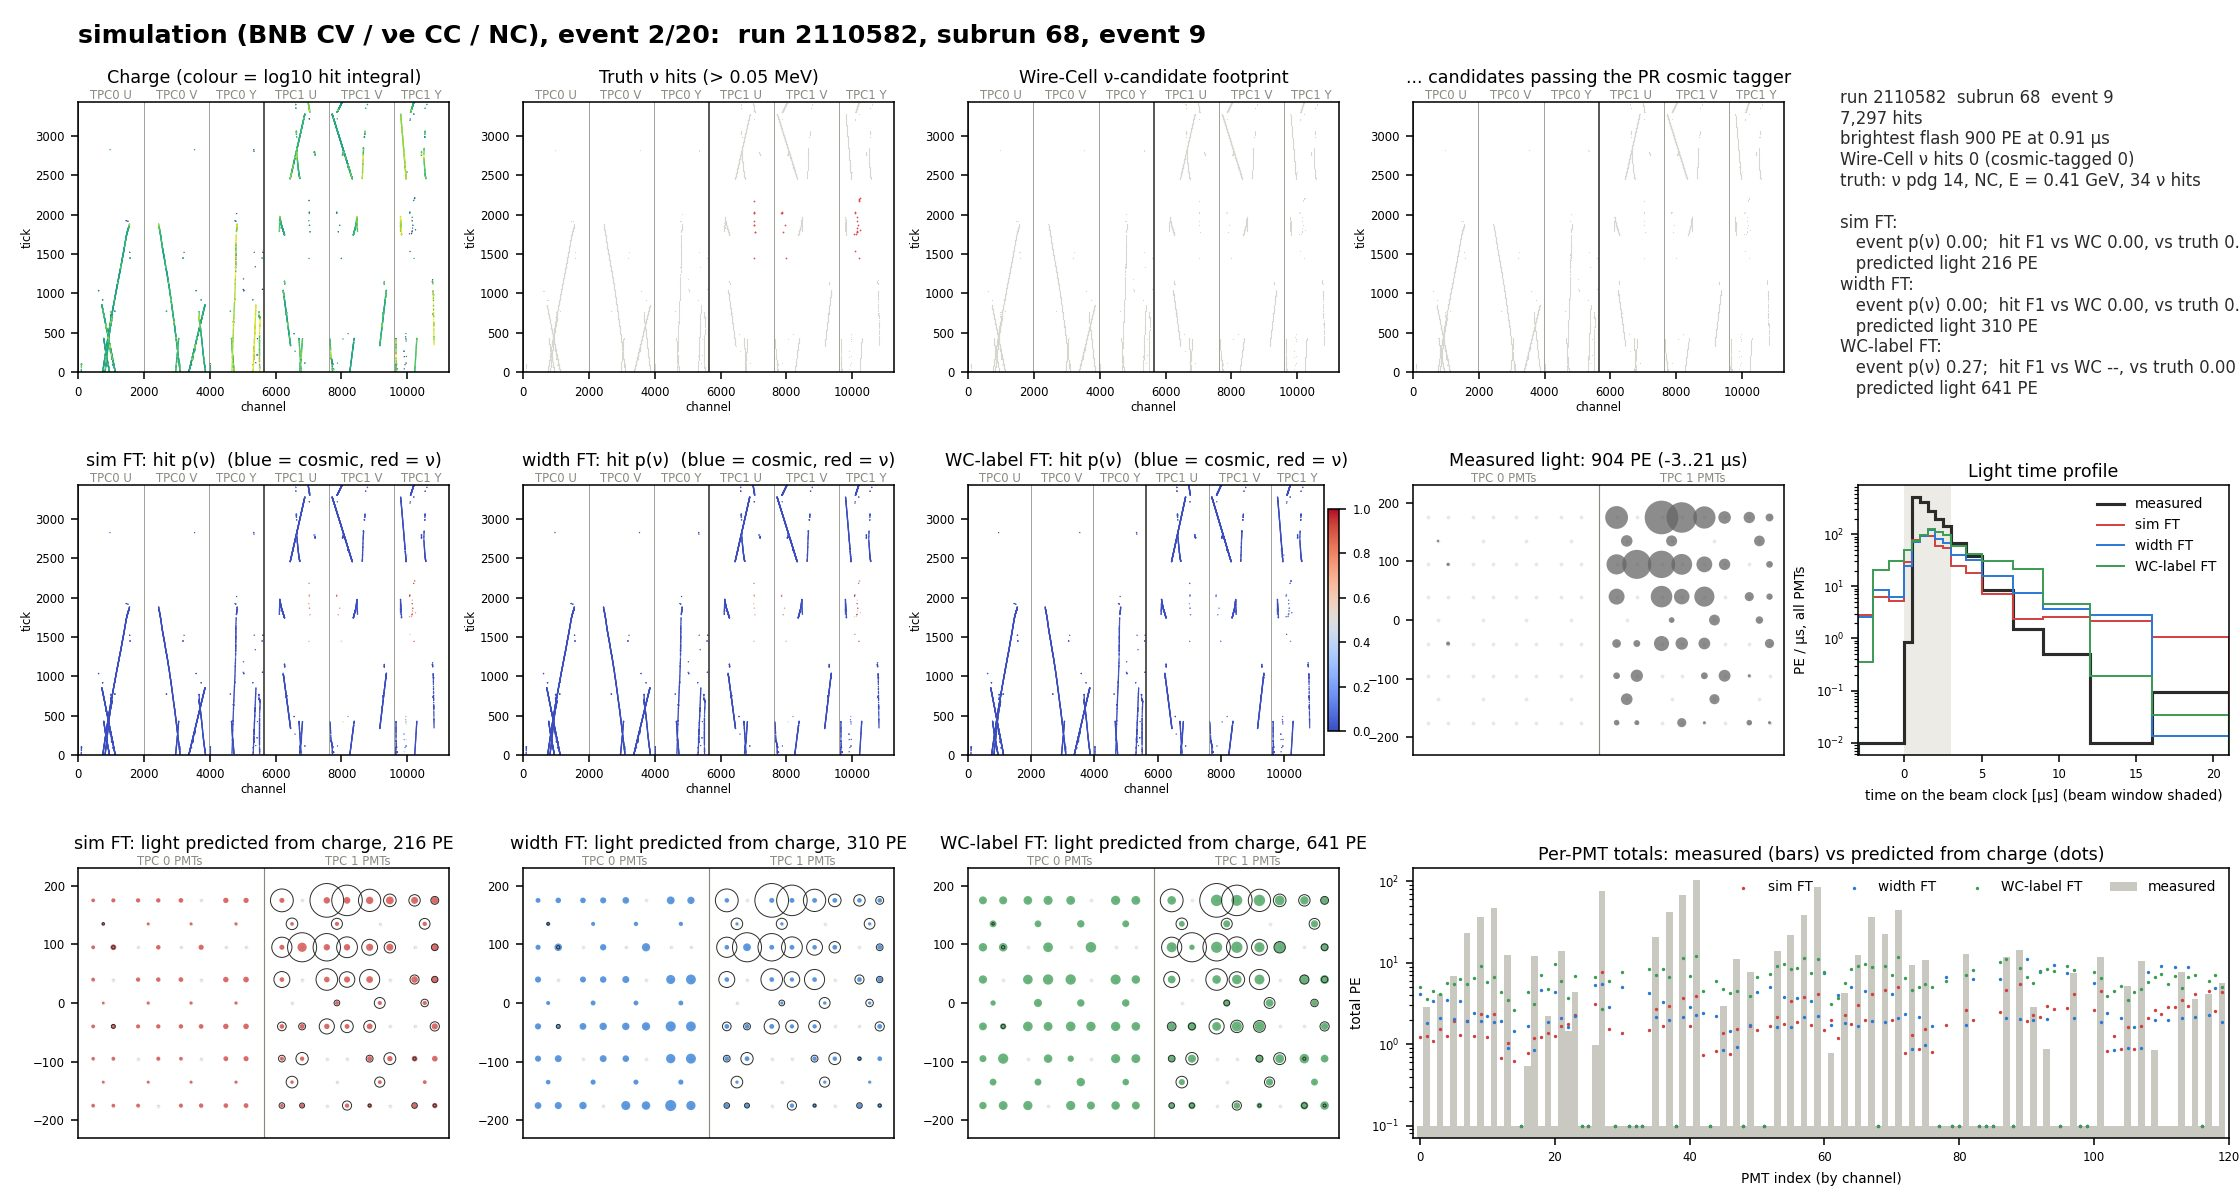
\includegraphics[width=\paperwidth,height=\paperheight,keepaspectratio]{displays/sim_01.jpg}}
\end{frame}
% Simulation 3/20: run 2105746, subrun 27, event 4; event p(nu): sim FT 1.00, width FT 1.00, WC-label FT 0.82
\begin{frame}[plain]
  \centering\vspace*{-2pt}
  \makebox[\linewidth][c]{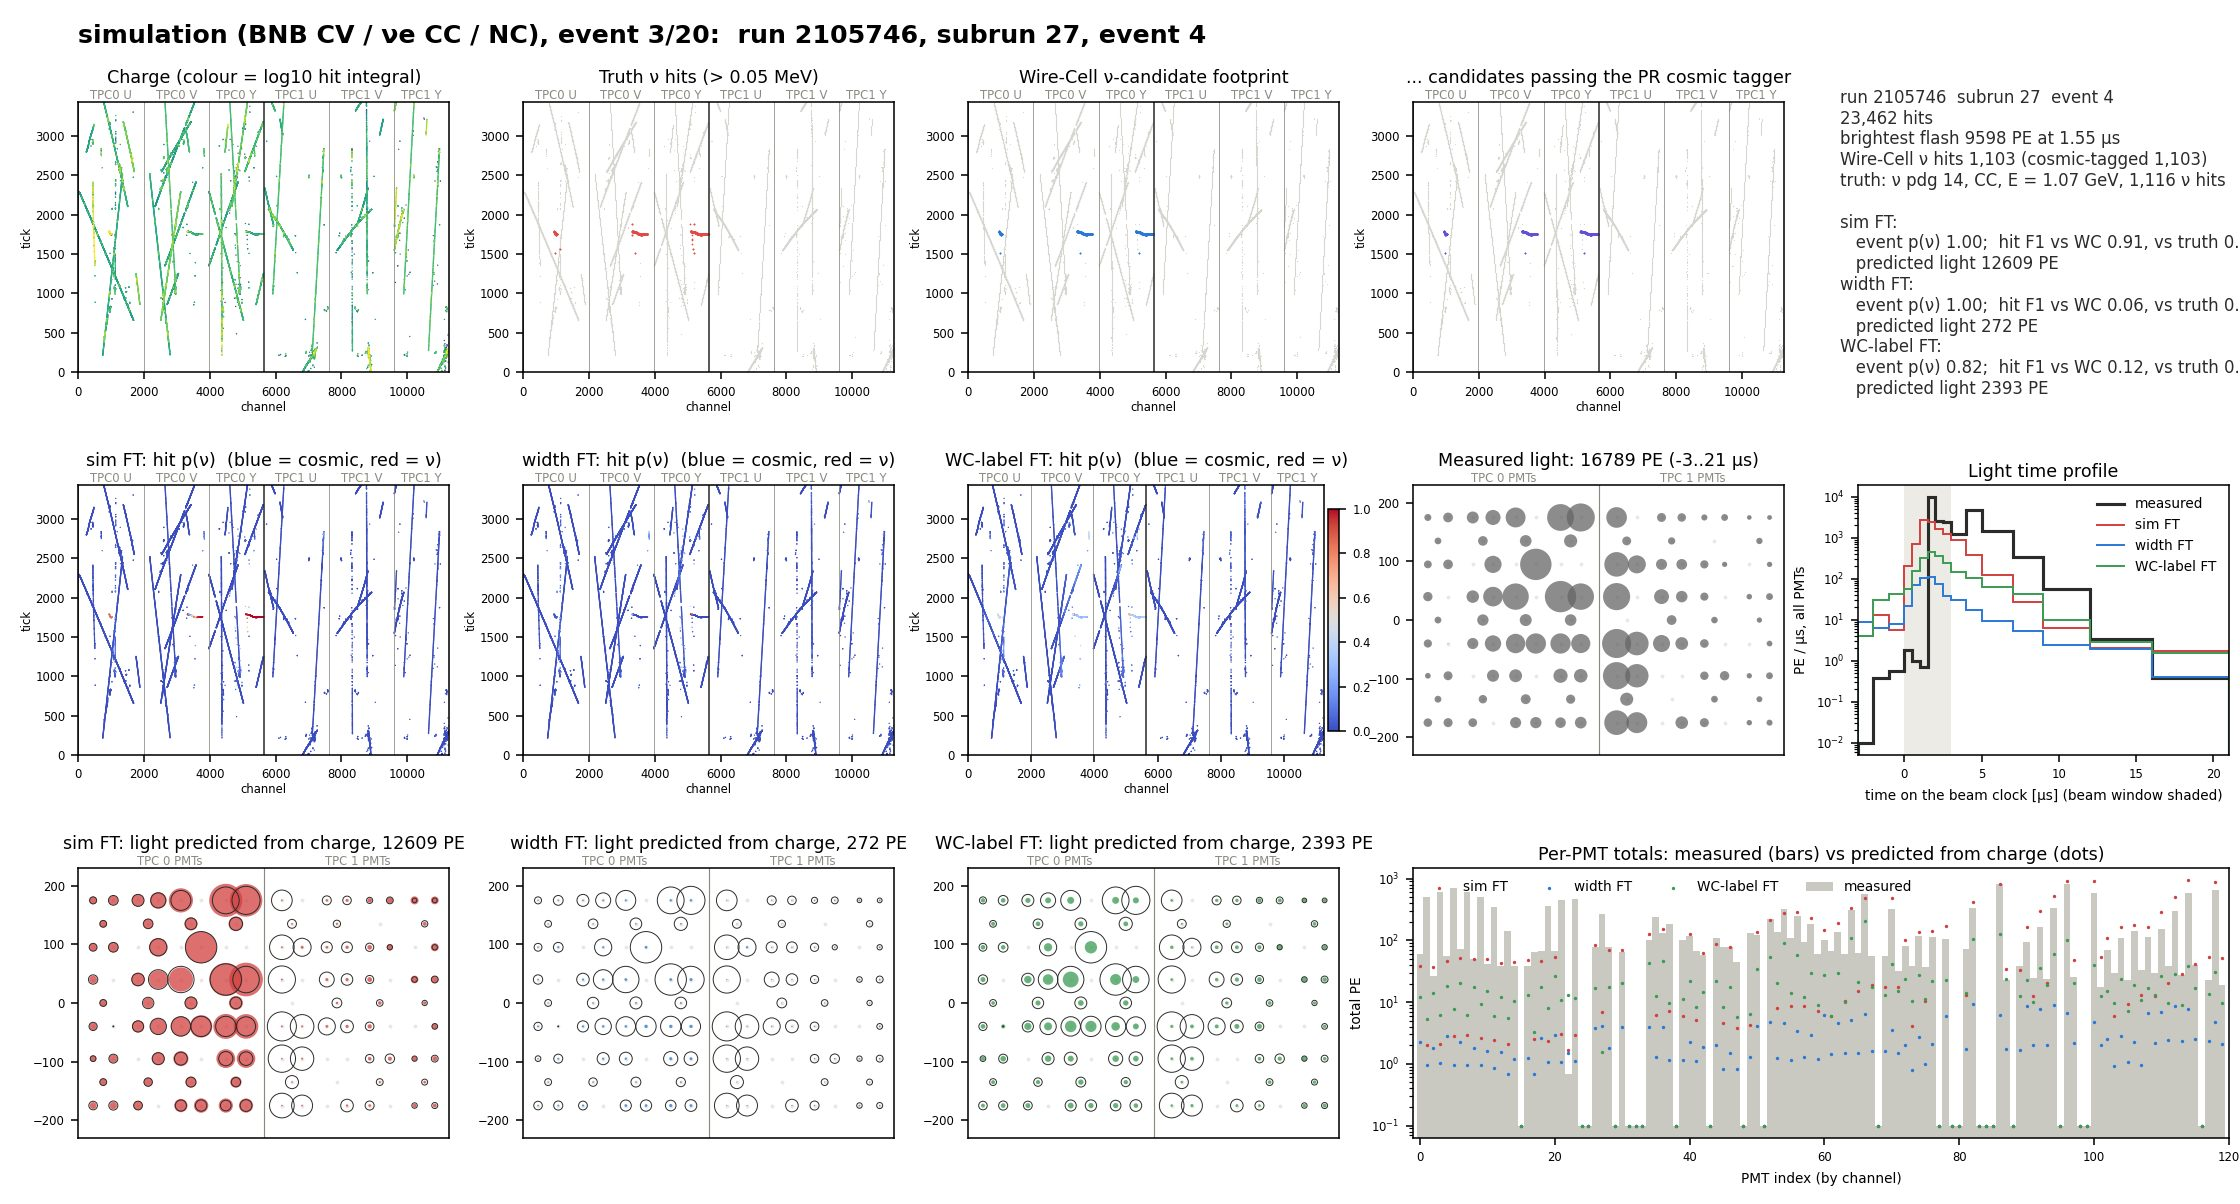
\includegraphics[width=\paperwidth,height=\paperheight,keepaspectratio]{displays/sim_02.jpg}}
\end{frame}
% Simulation 4/20: run 2105310, subrun 82, event 6; event p(nu): sim FT 1.00, width FT 1.00, WC-label FT 0.98
\begin{frame}[plain]
  \centering\vspace*{-2pt}
  \makebox[\linewidth][c]{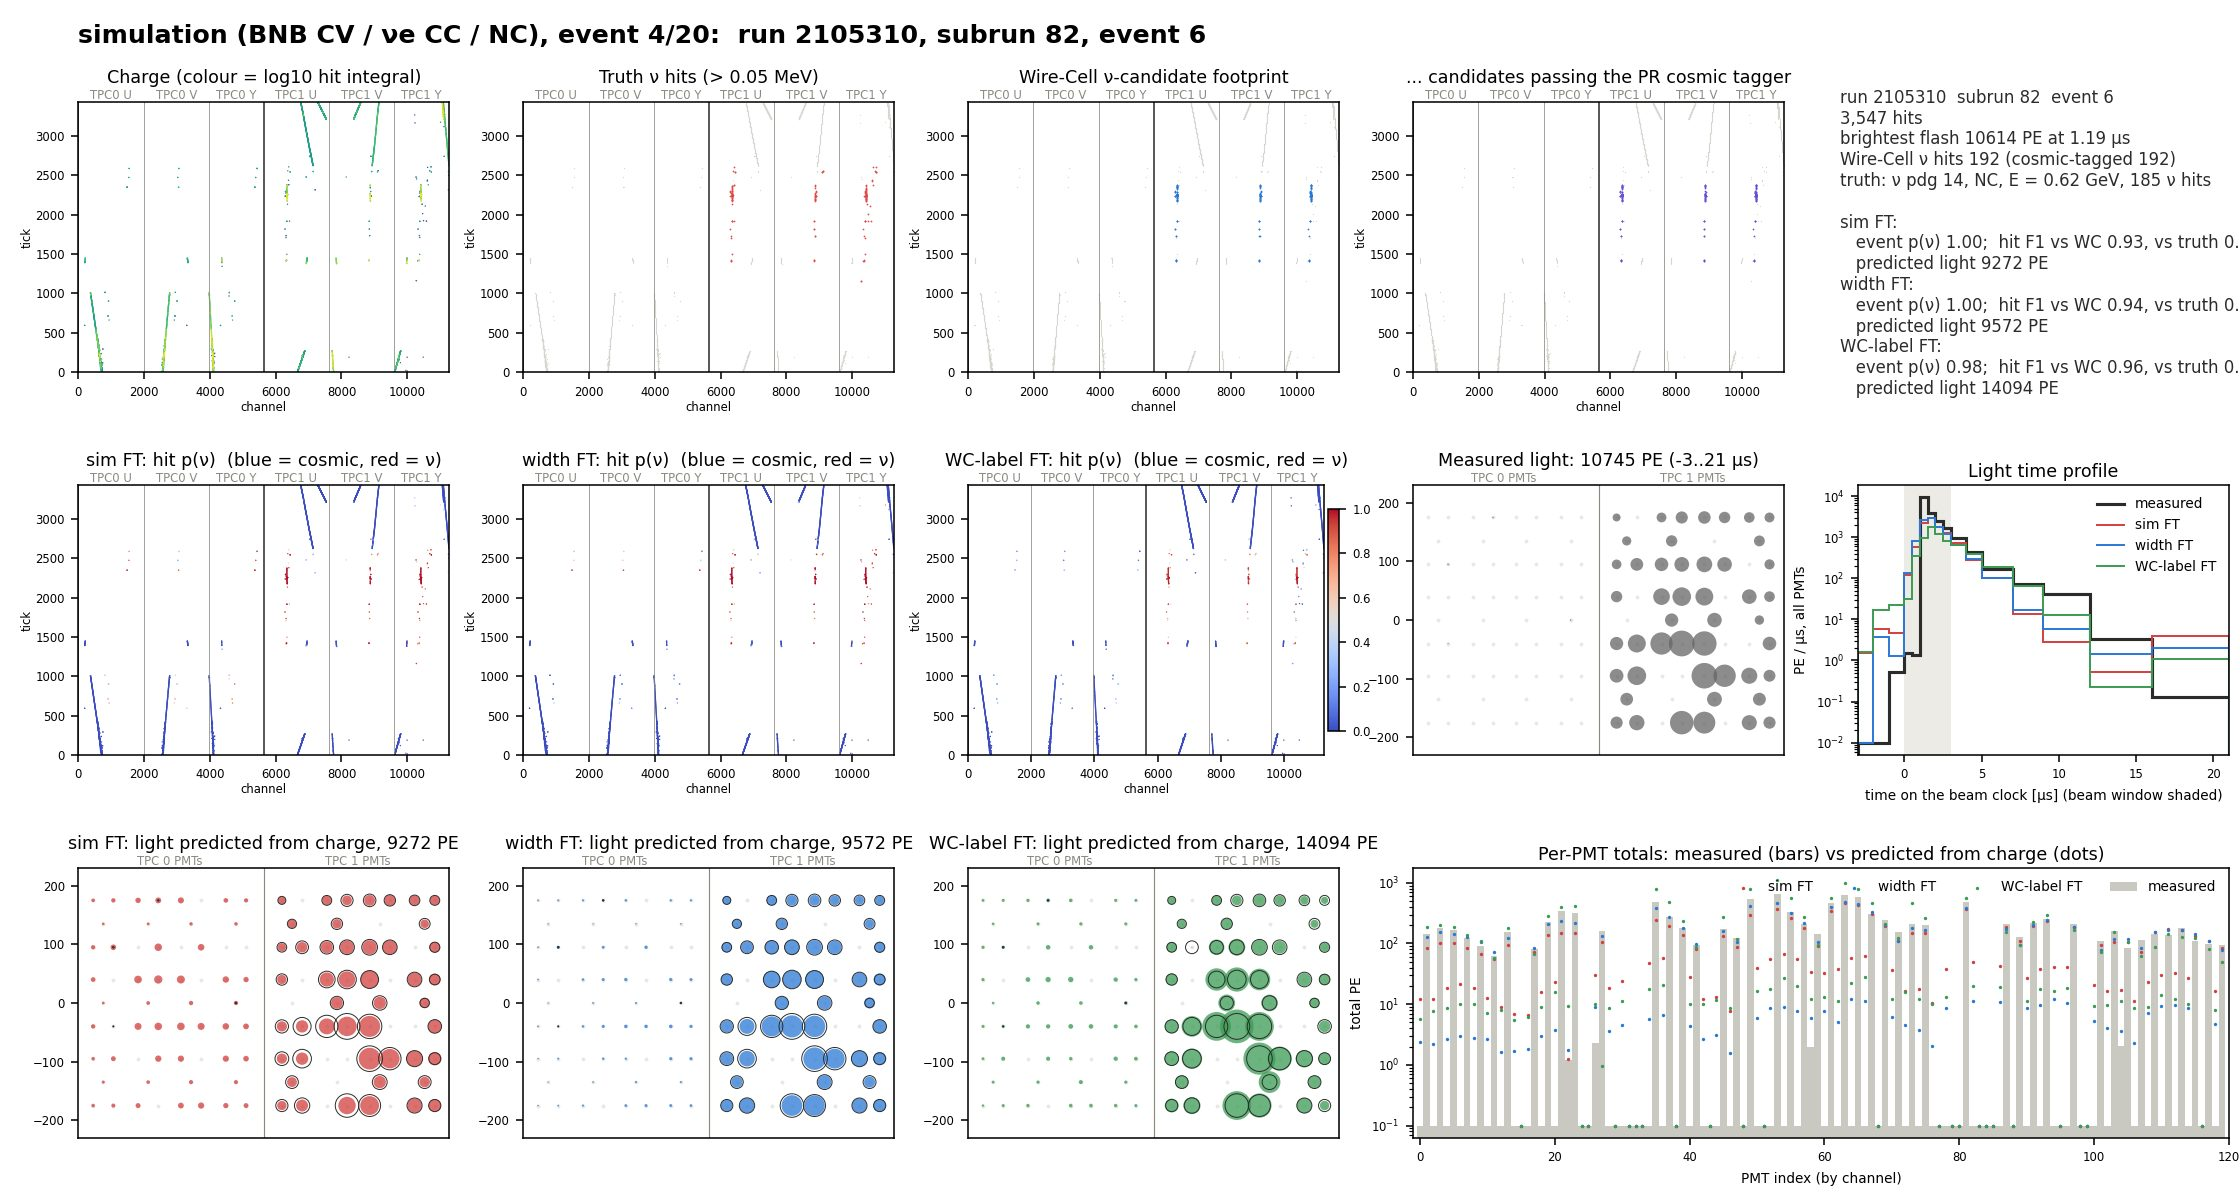
\includegraphics[width=\paperwidth,height=\paperheight,keepaspectratio]{displays/sim_03.jpg}}
\end{frame}
% Simulation 5/20: run 2105113, subrun 8, event 5; event p(nu): sim FT 1.00, width FT 1.00, WC-label FT 0.97
\begin{frame}[plain]
  \centering\vspace*{-2pt}
  \makebox[\linewidth][c]{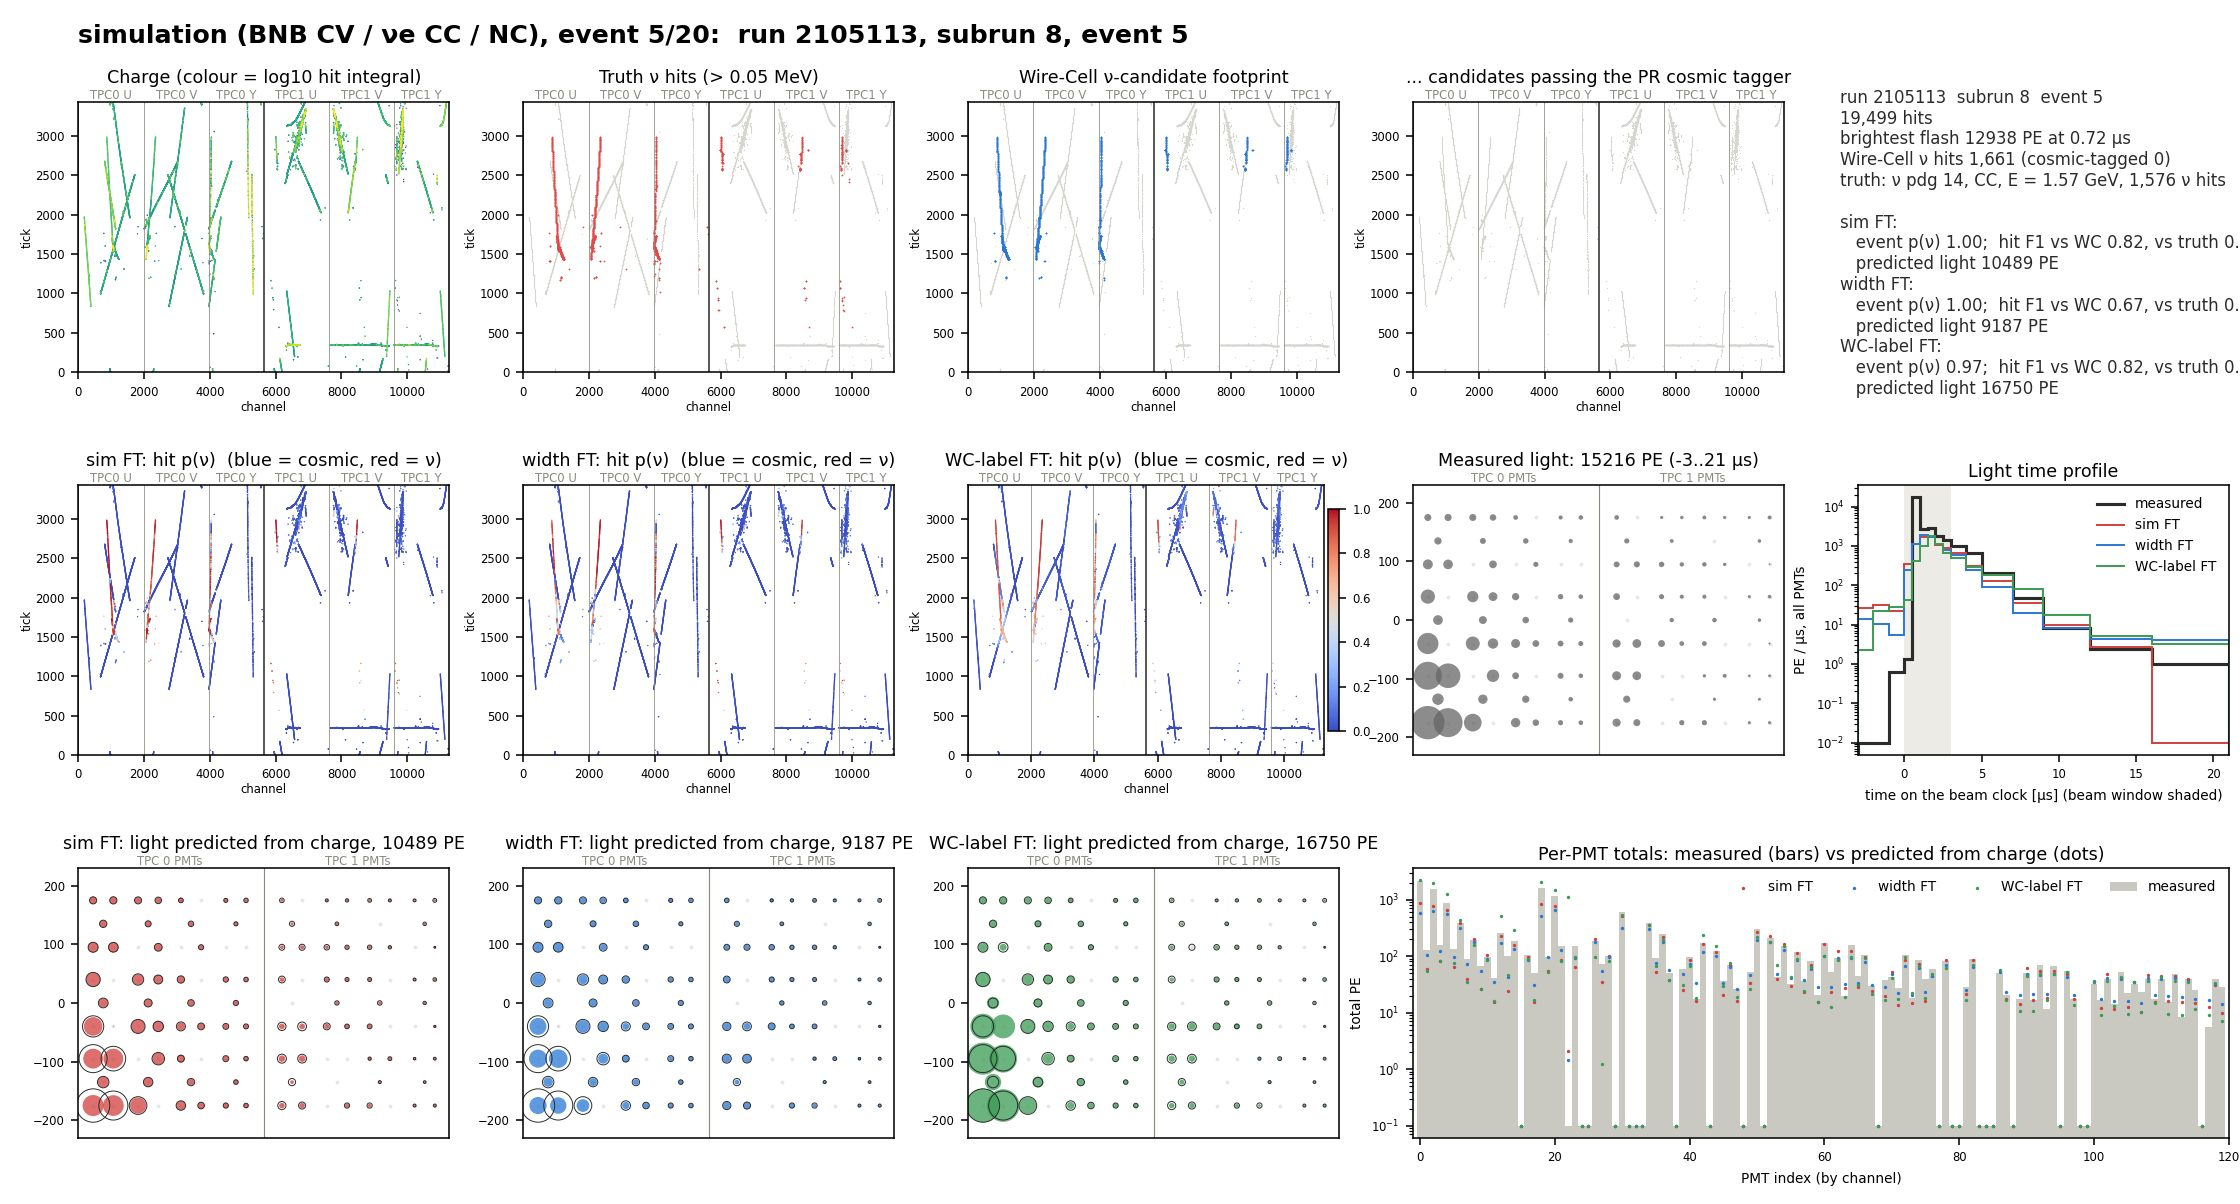
\includegraphics[width=\paperwidth,height=\paperheight,keepaspectratio]{displays/sim_04.jpg}}
\end{frame}
% Simulation 6/20: run 2105075, subrun 93, event 7; event p(nu): sim FT 1.00, width FT 1.00, WC-label FT 0.98
\begin{frame}[plain]
  \centering\vspace*{-2pt}
  \makebox[\linewidth][c]{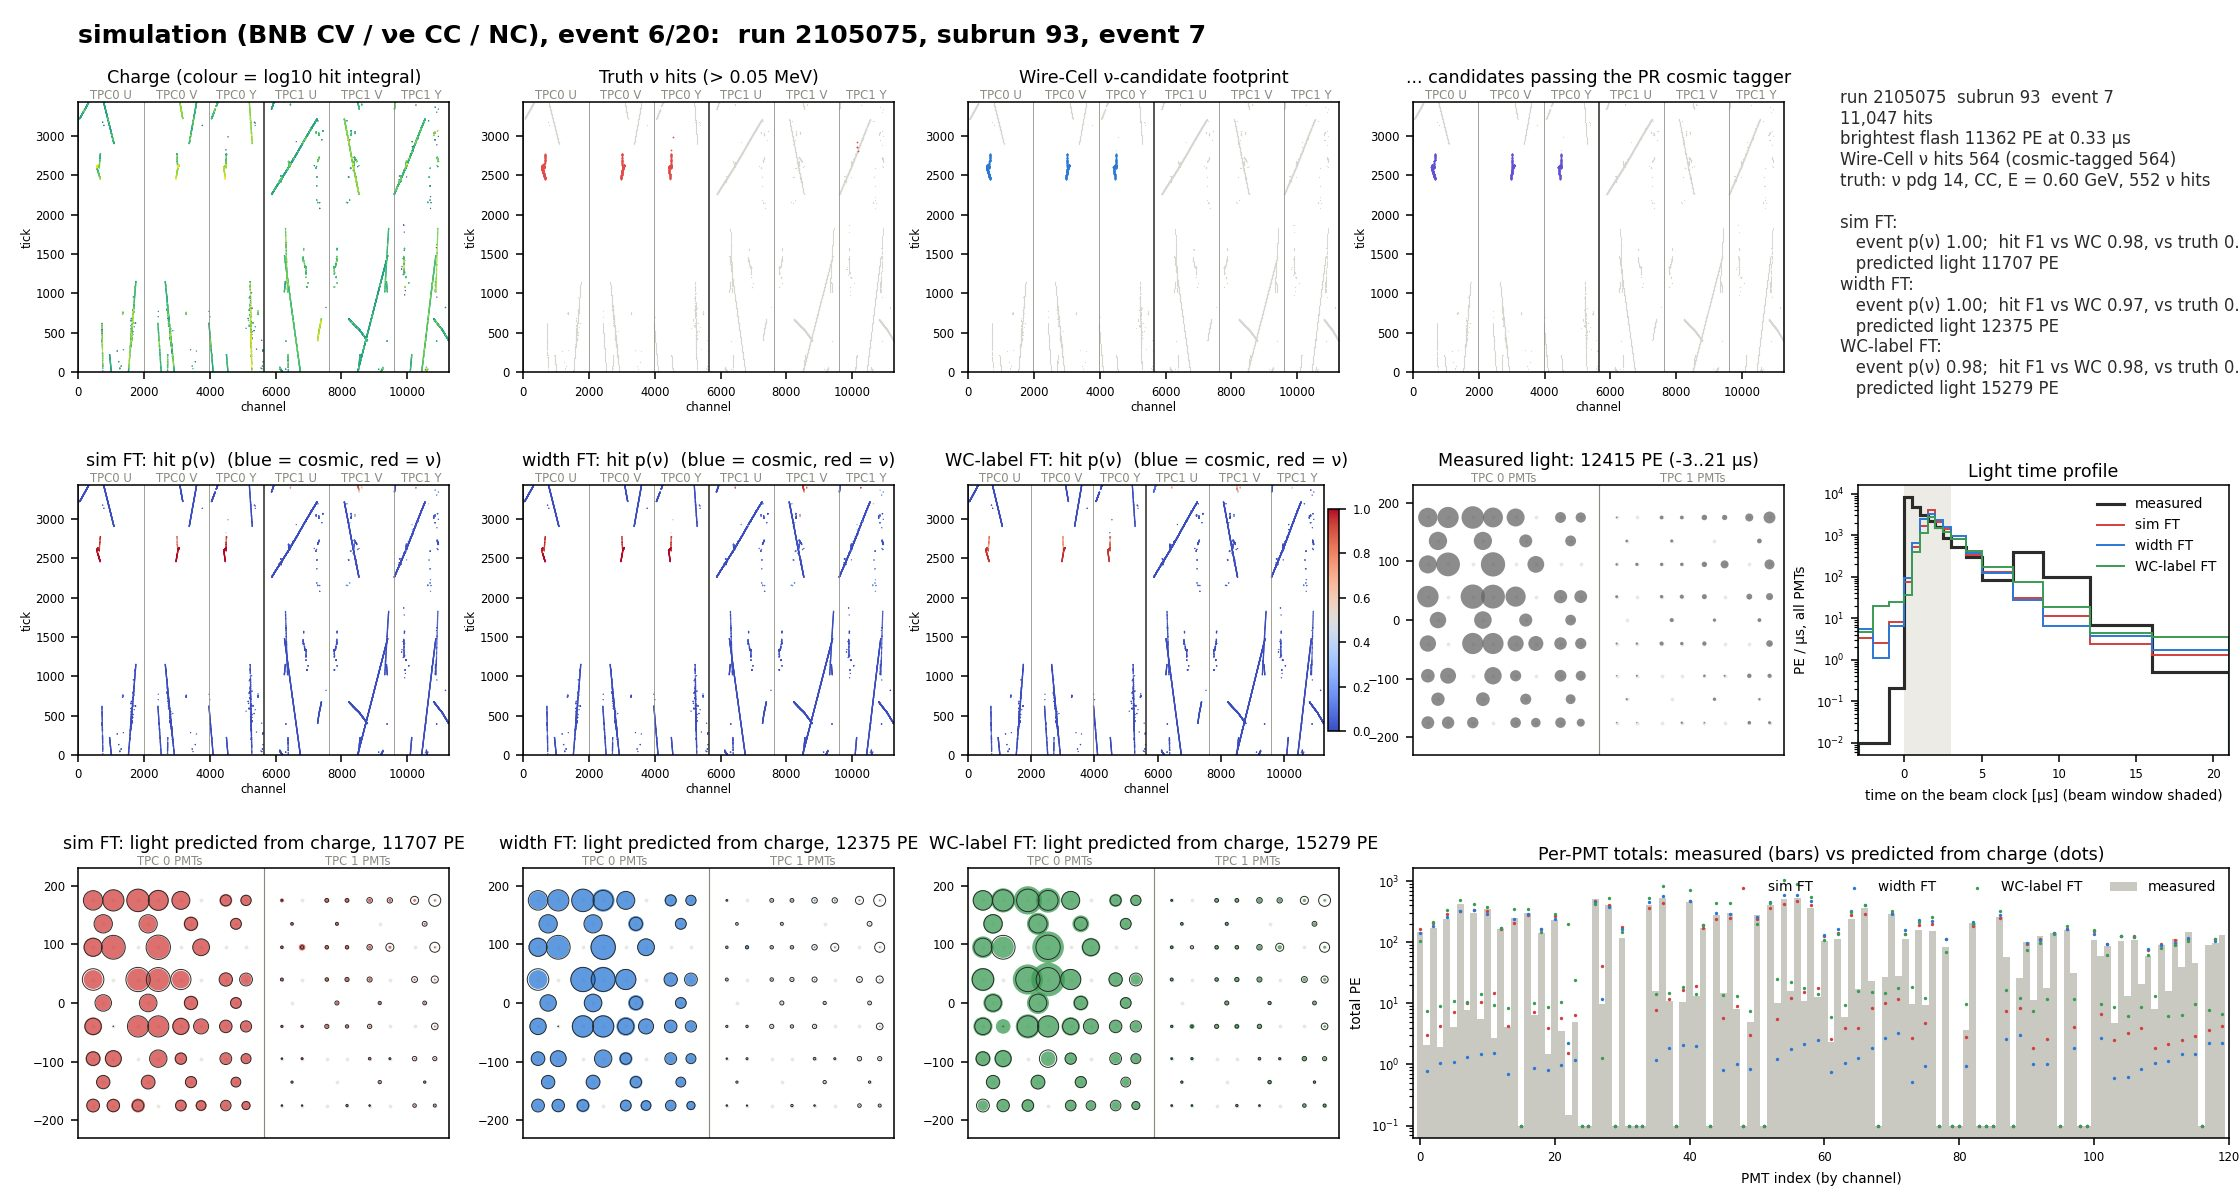
\includegraphics[width=\paperwidth,height=\paperheight,keepaspectratio]{displays/sim_05.jpg}}
\end{frame}
% Simulation 7/20: run 2100060, subrun 93, event 5; event p(nu): sim FT 1.00, width FT 0.16, WC-label FT 0.61
\begin{frame}[plain]
  \centering\vspace*{-2pt}
  \makebox[\linewidth][c]{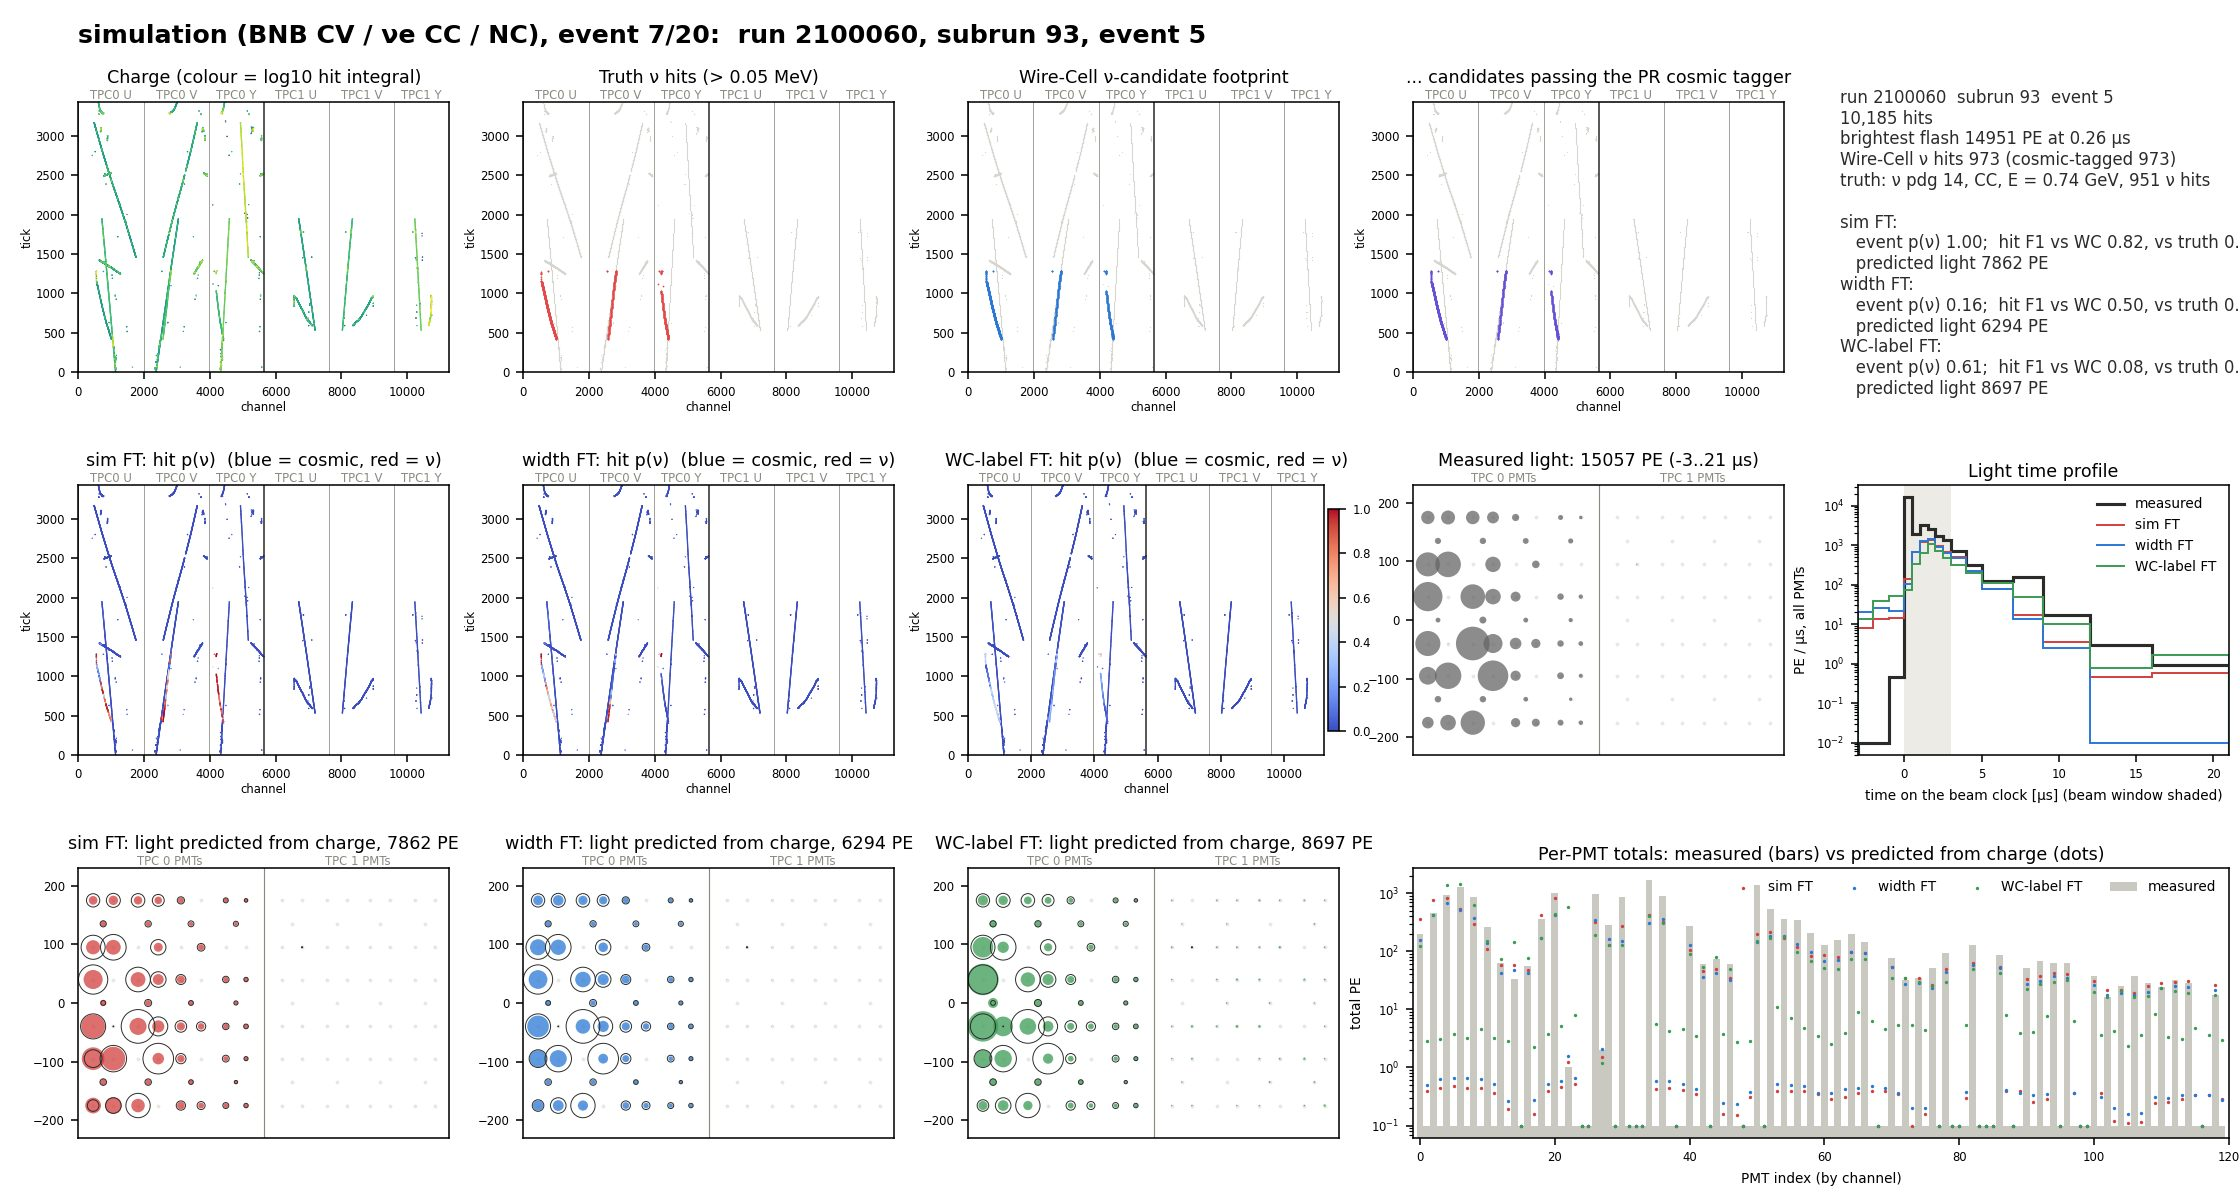
\includegraphics[width=\paperwidth,height=\paperheight,keepaspectratio]{displays/sim_06.jpg}}
\end{frame}
% Simulation 8/20: run 2100197, subrun 83, event 1; event p(nu): sim FT 1.00, width FT 1.00, WC-label FT 0.94
\begin{frame}[plain]
  \centering\vspace*{-2pt}
  \makebox[\linewidth][c]{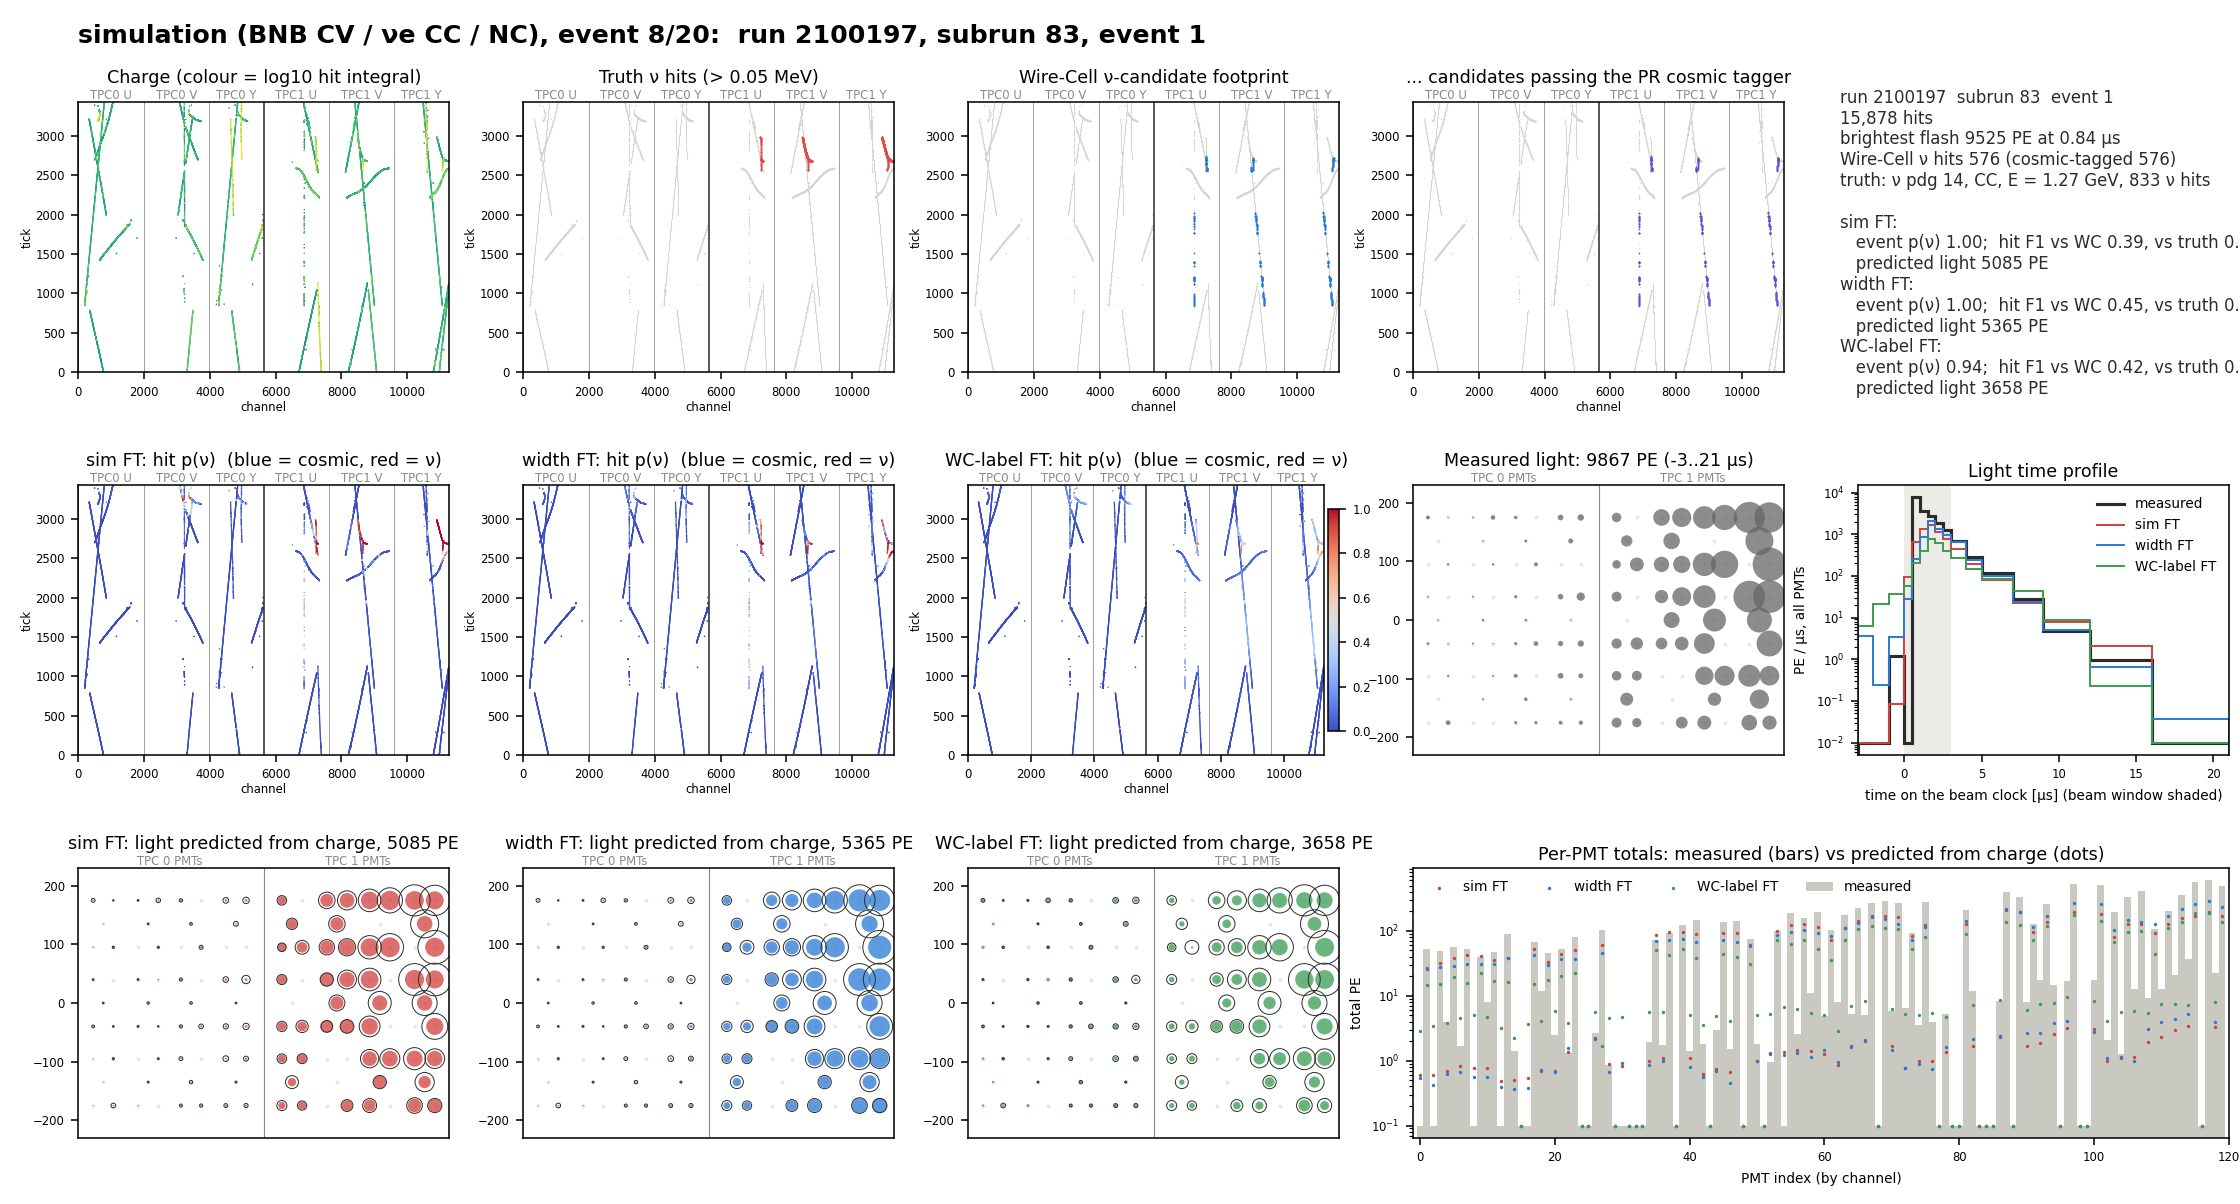
\includegraphics[width=\paperwidth,height=\paperheight,keepaspectratio]{displays/sim_07.jpg}}
\end{frame}
% Simulation 9/20: run 2100328, subrun 6, event 6; event p(nu): sim FT 1.00, width FT 1.00, WC-label FT 0.88
\begin{frame}[plain]
  \centering\vspace*{-2pt}
  \makebox[\linewidth][c]{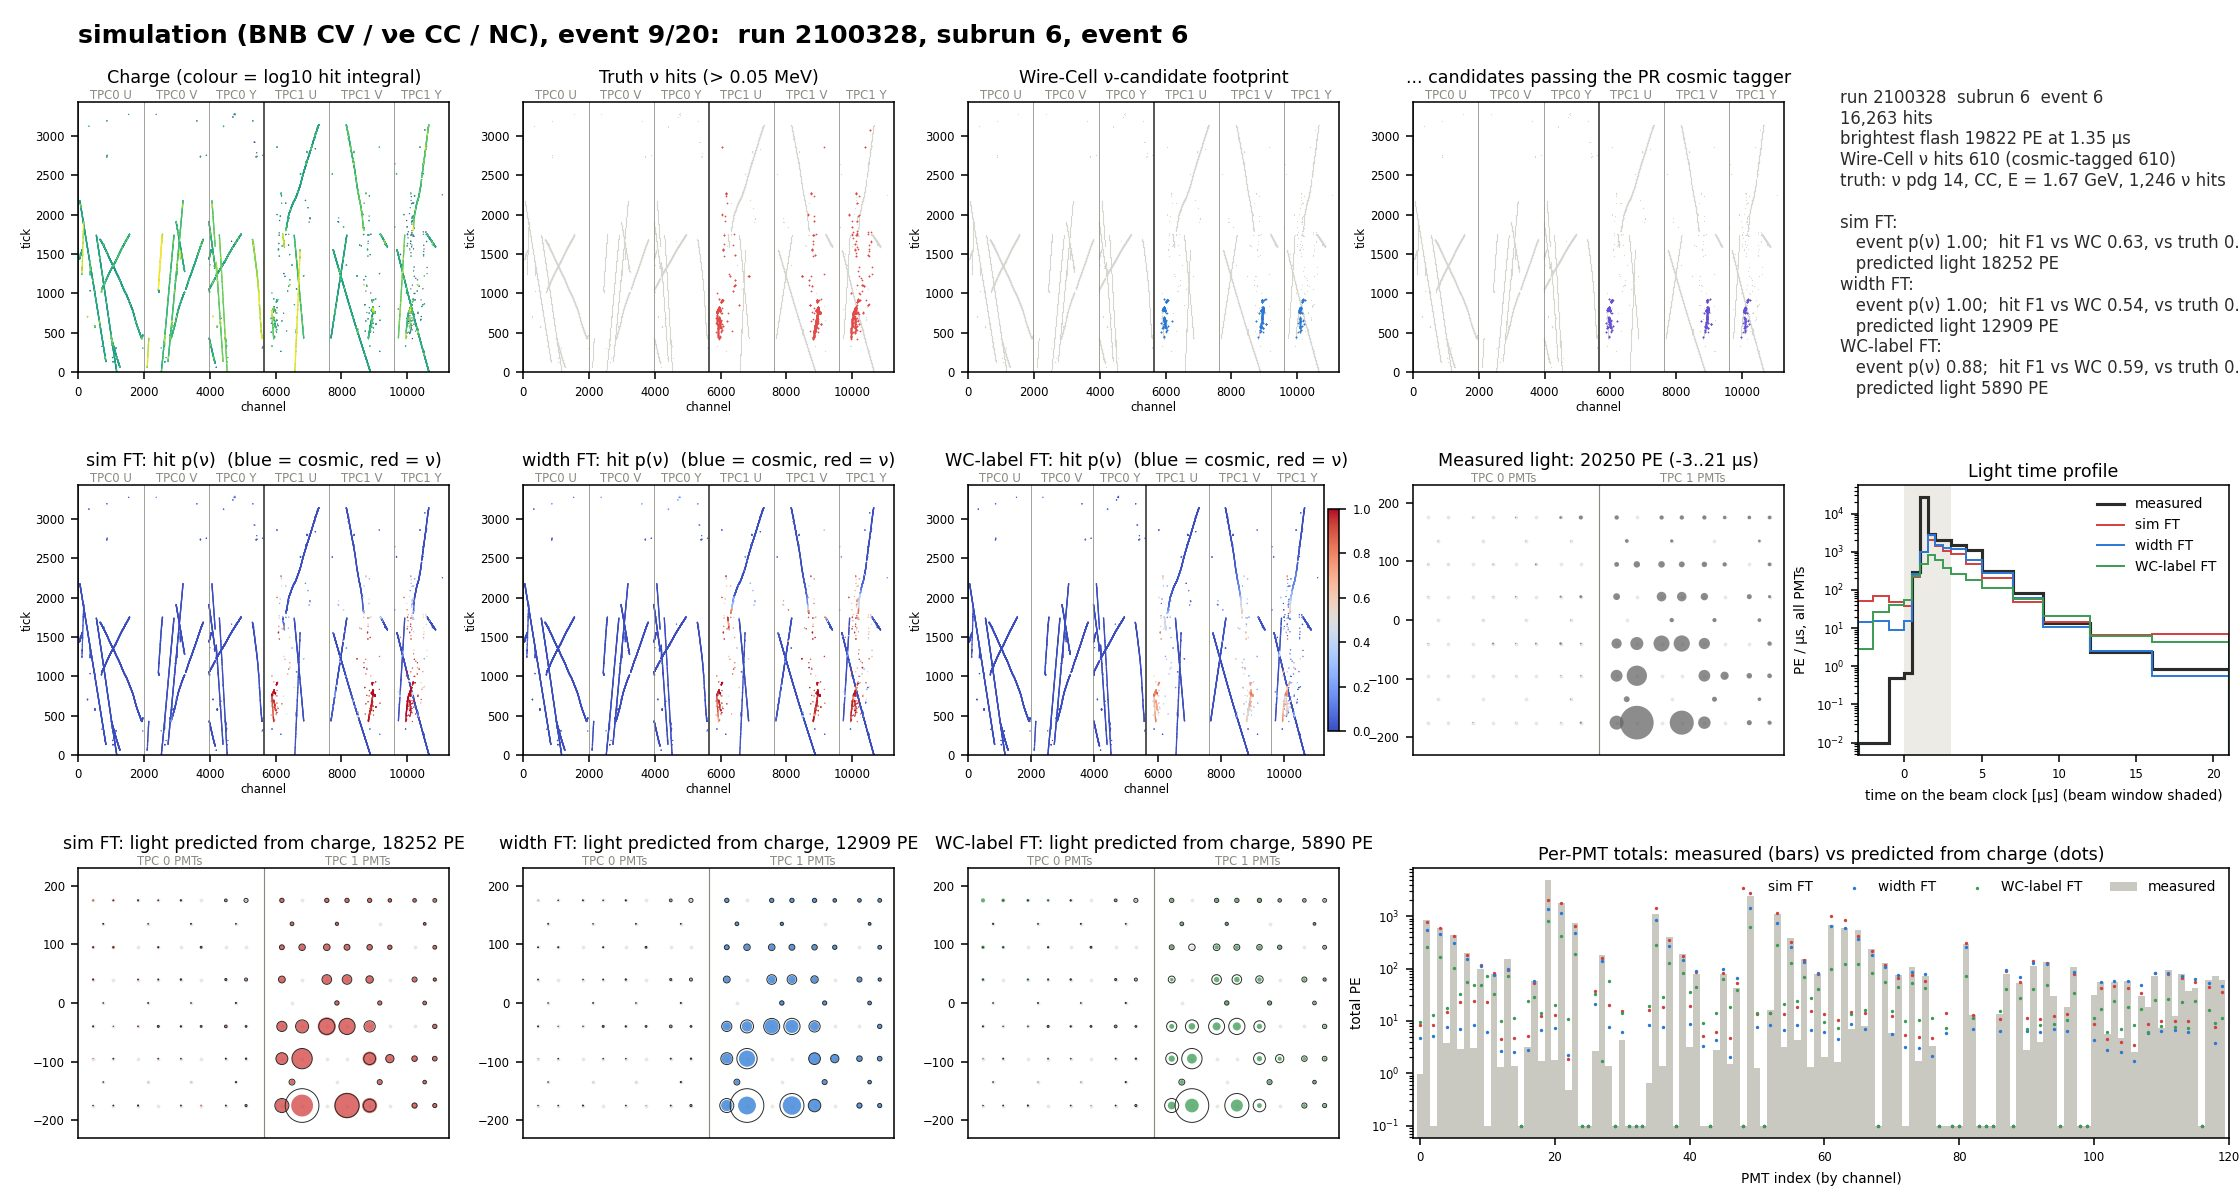
\includegraphics[width=\paperwidth,height=\paperheight,keepaspectratio]{displays/sim_08.jpg}}
\end{frame}
% Simulation 10/20: run 2100281, subrun 77, event 4; event p(nu): sim FT 0.00, width FT 0.00, WC-label FT 0.02
\begin{frame}[plain]
  \centering\vspace*{-2pt}
  \makebox[\linewidth][c]{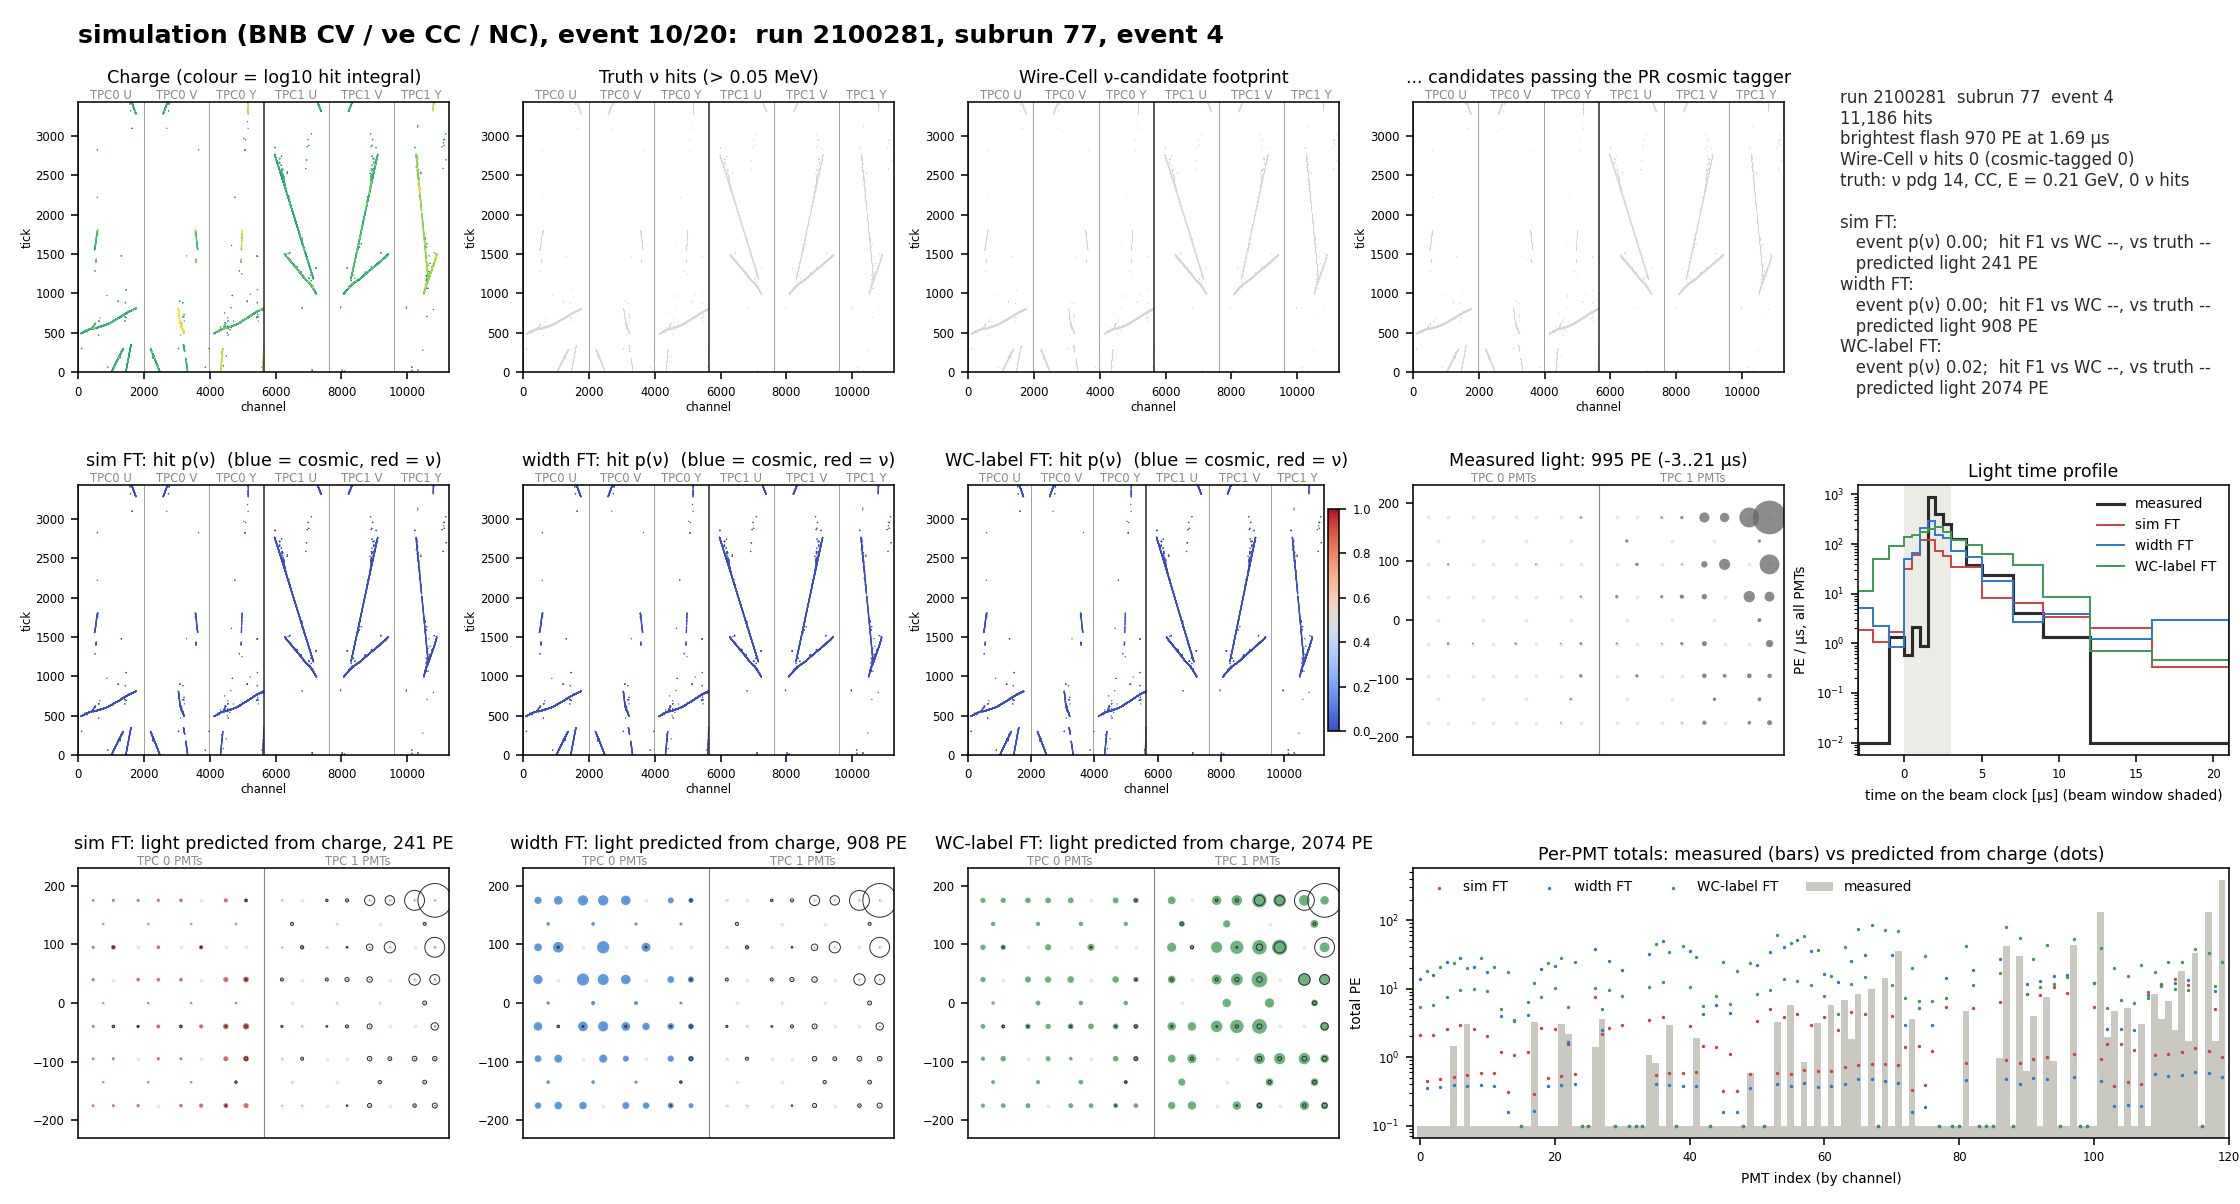
\includegraphics[width=\paperwidth,height=\paperheight,keepaspectratio]{displays/sim_09.jpg}}
\end{frame}
% Simulation 11/20: run 6708895, subrun 84, event 24; event p(nu): sim FT 1.00, width FT 1.00, WC-label FT 0.98
\begin{frame}[plain]
  \centering\vspace*{-2pt}
  \makebox[\linewidth][c]{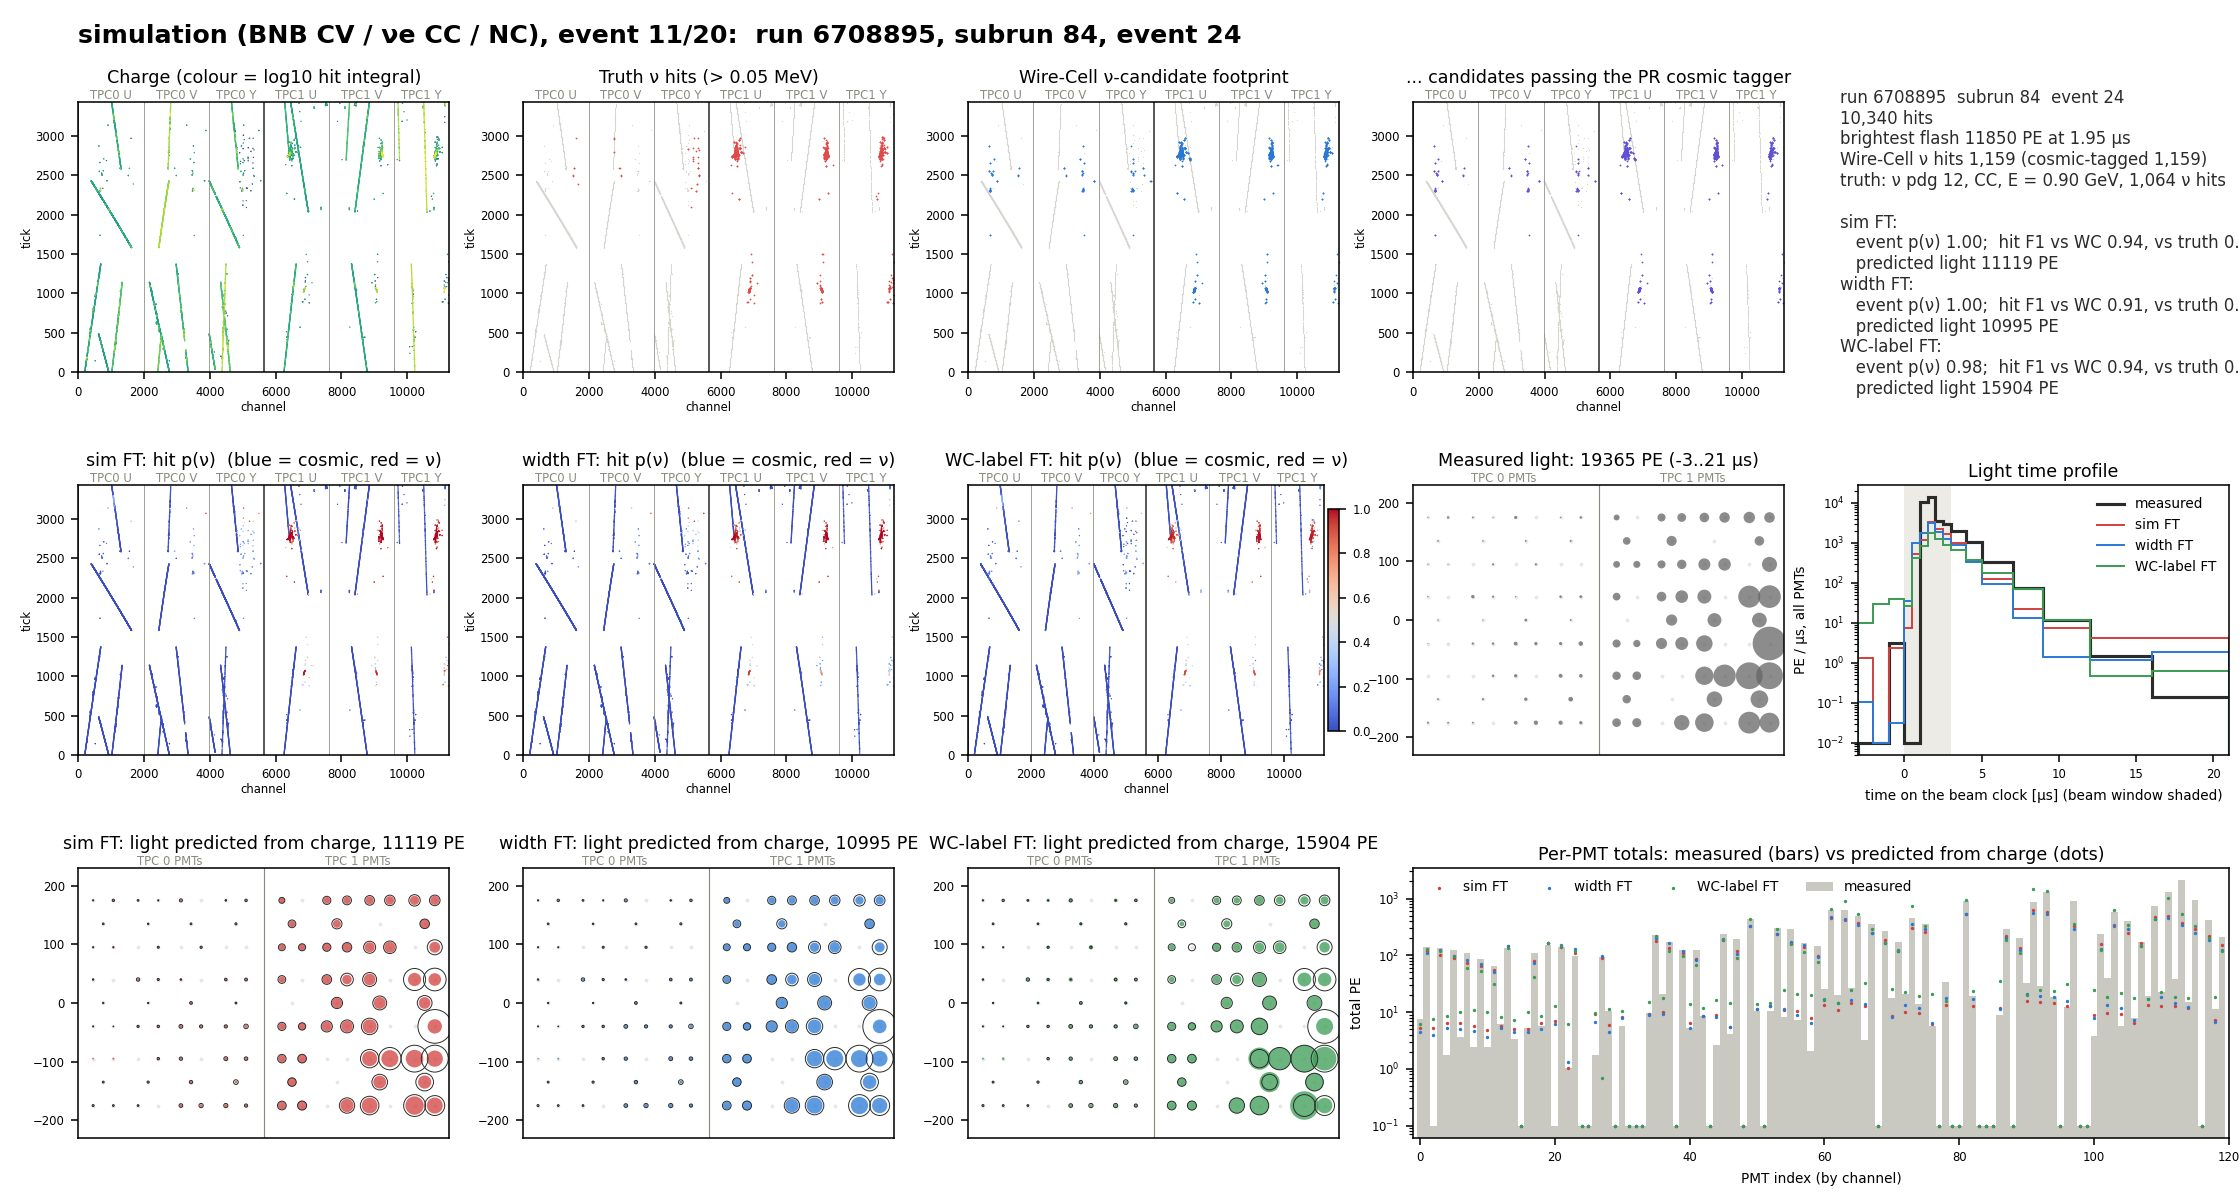
\includegraphics[width=\paperwidth,height=\paperheight,keepaspectratio]{displays/sim_10.jpg}}
\end{frame}
% Simulation 12/20: run 6709684, subrun 21, event 109; event p(nu): sim FT 1.00, width FT 1.00, WC-label FT 0.94
\begin{frame}[plain]
  \centering\vspace*{-2pt}
  \makebox[\linewidth][c]{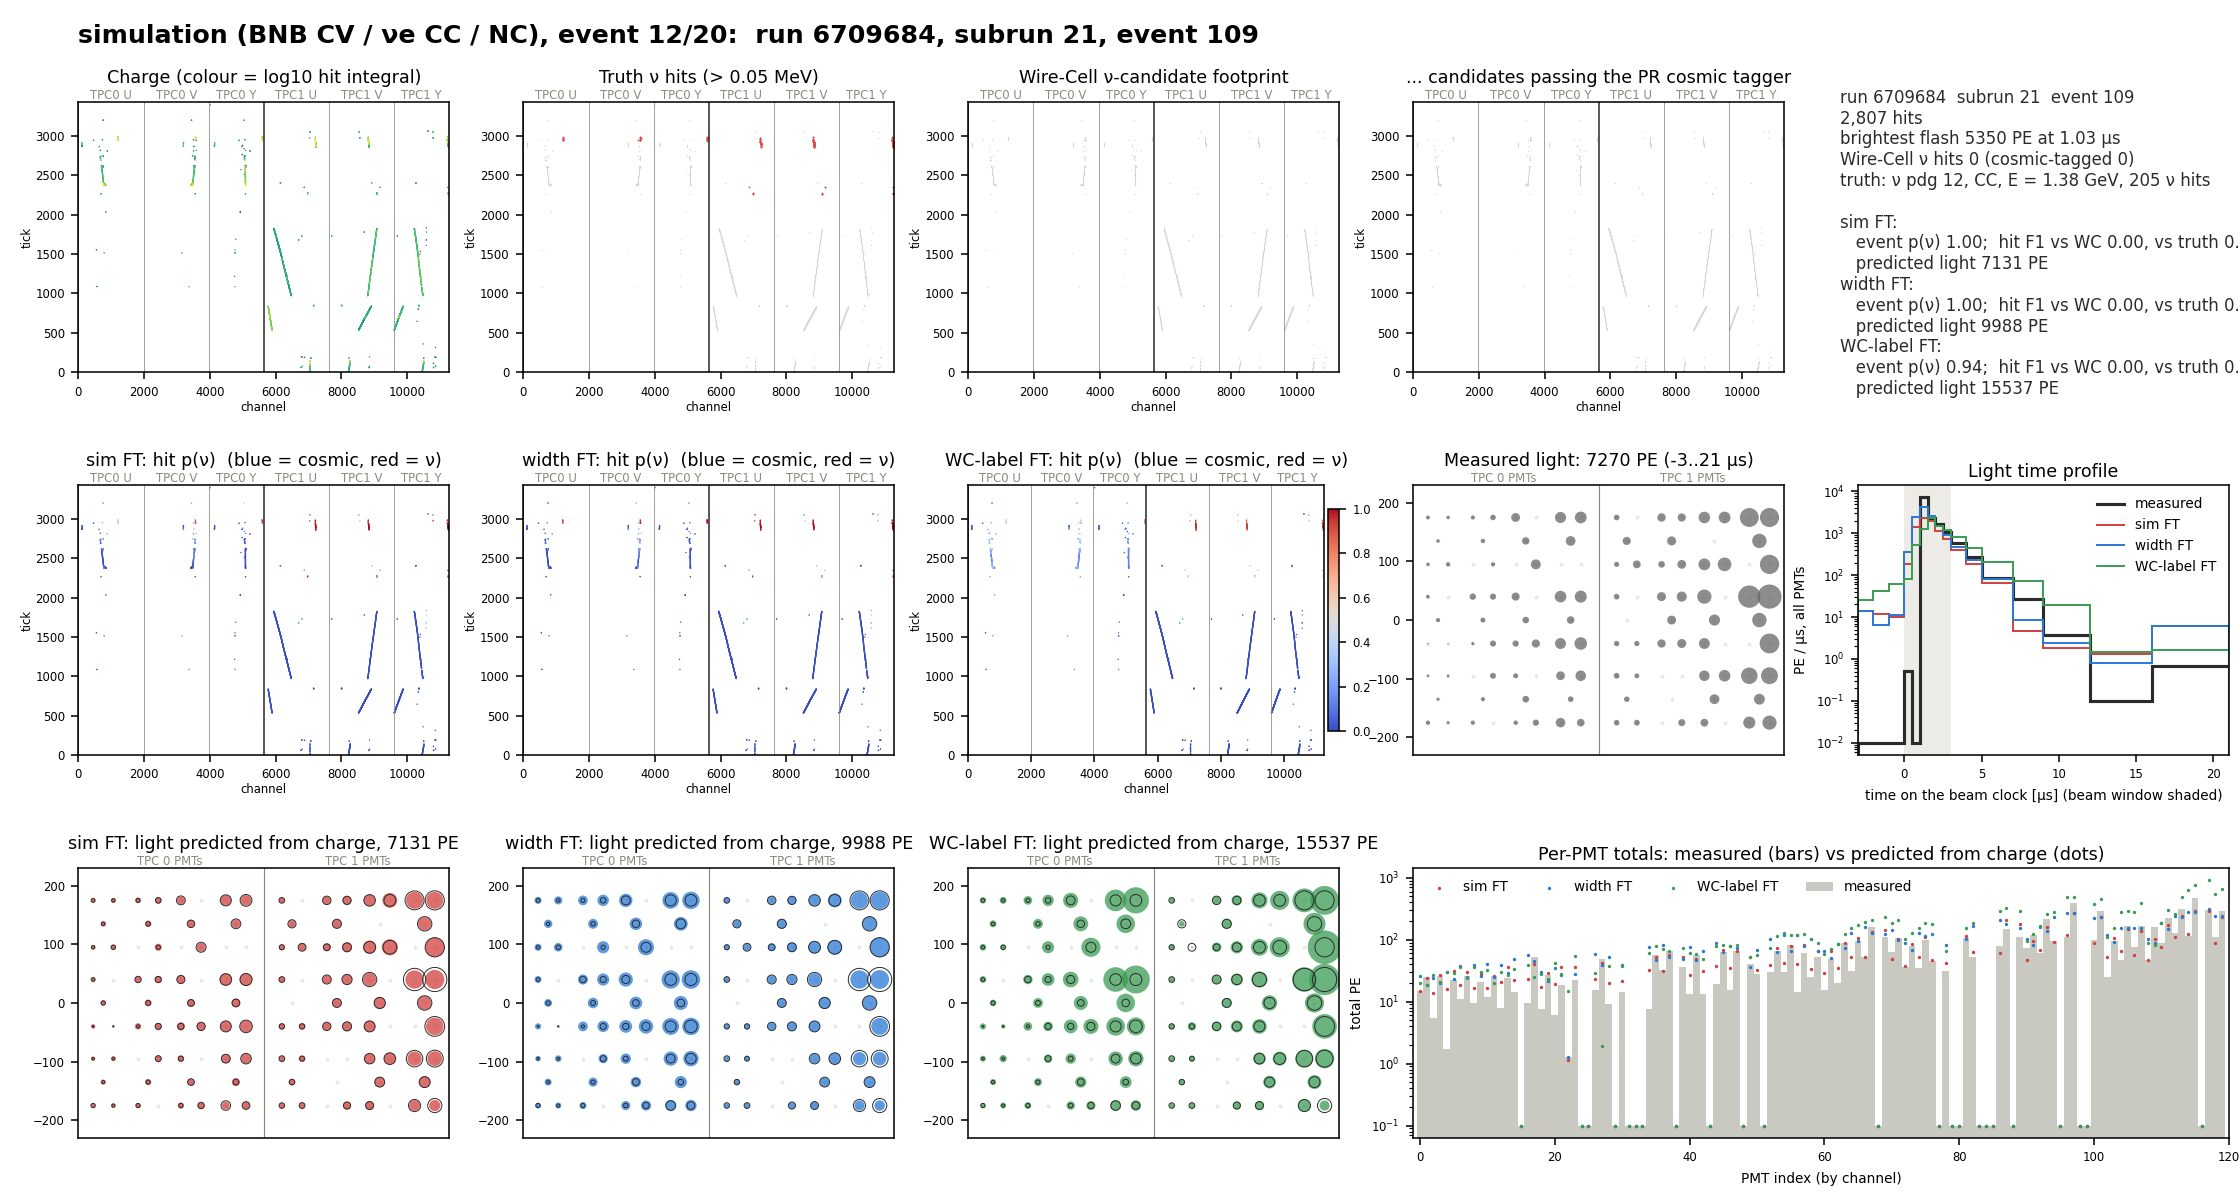
\includegraphics[width=\paperwidth,height=\paperheight,keepaspectratio]{displays/sim_11.jpg}}
\end{frame}
% Simulation 13/20: run 6725872, subrun 6, event 39; event p(nu): sim FT 1.00, width FT 1.00, WC-label FT 0.98
\begin{frame}[plain]
  \centering\vspace*{-2pt}
  \makebox[\linewidth][c]{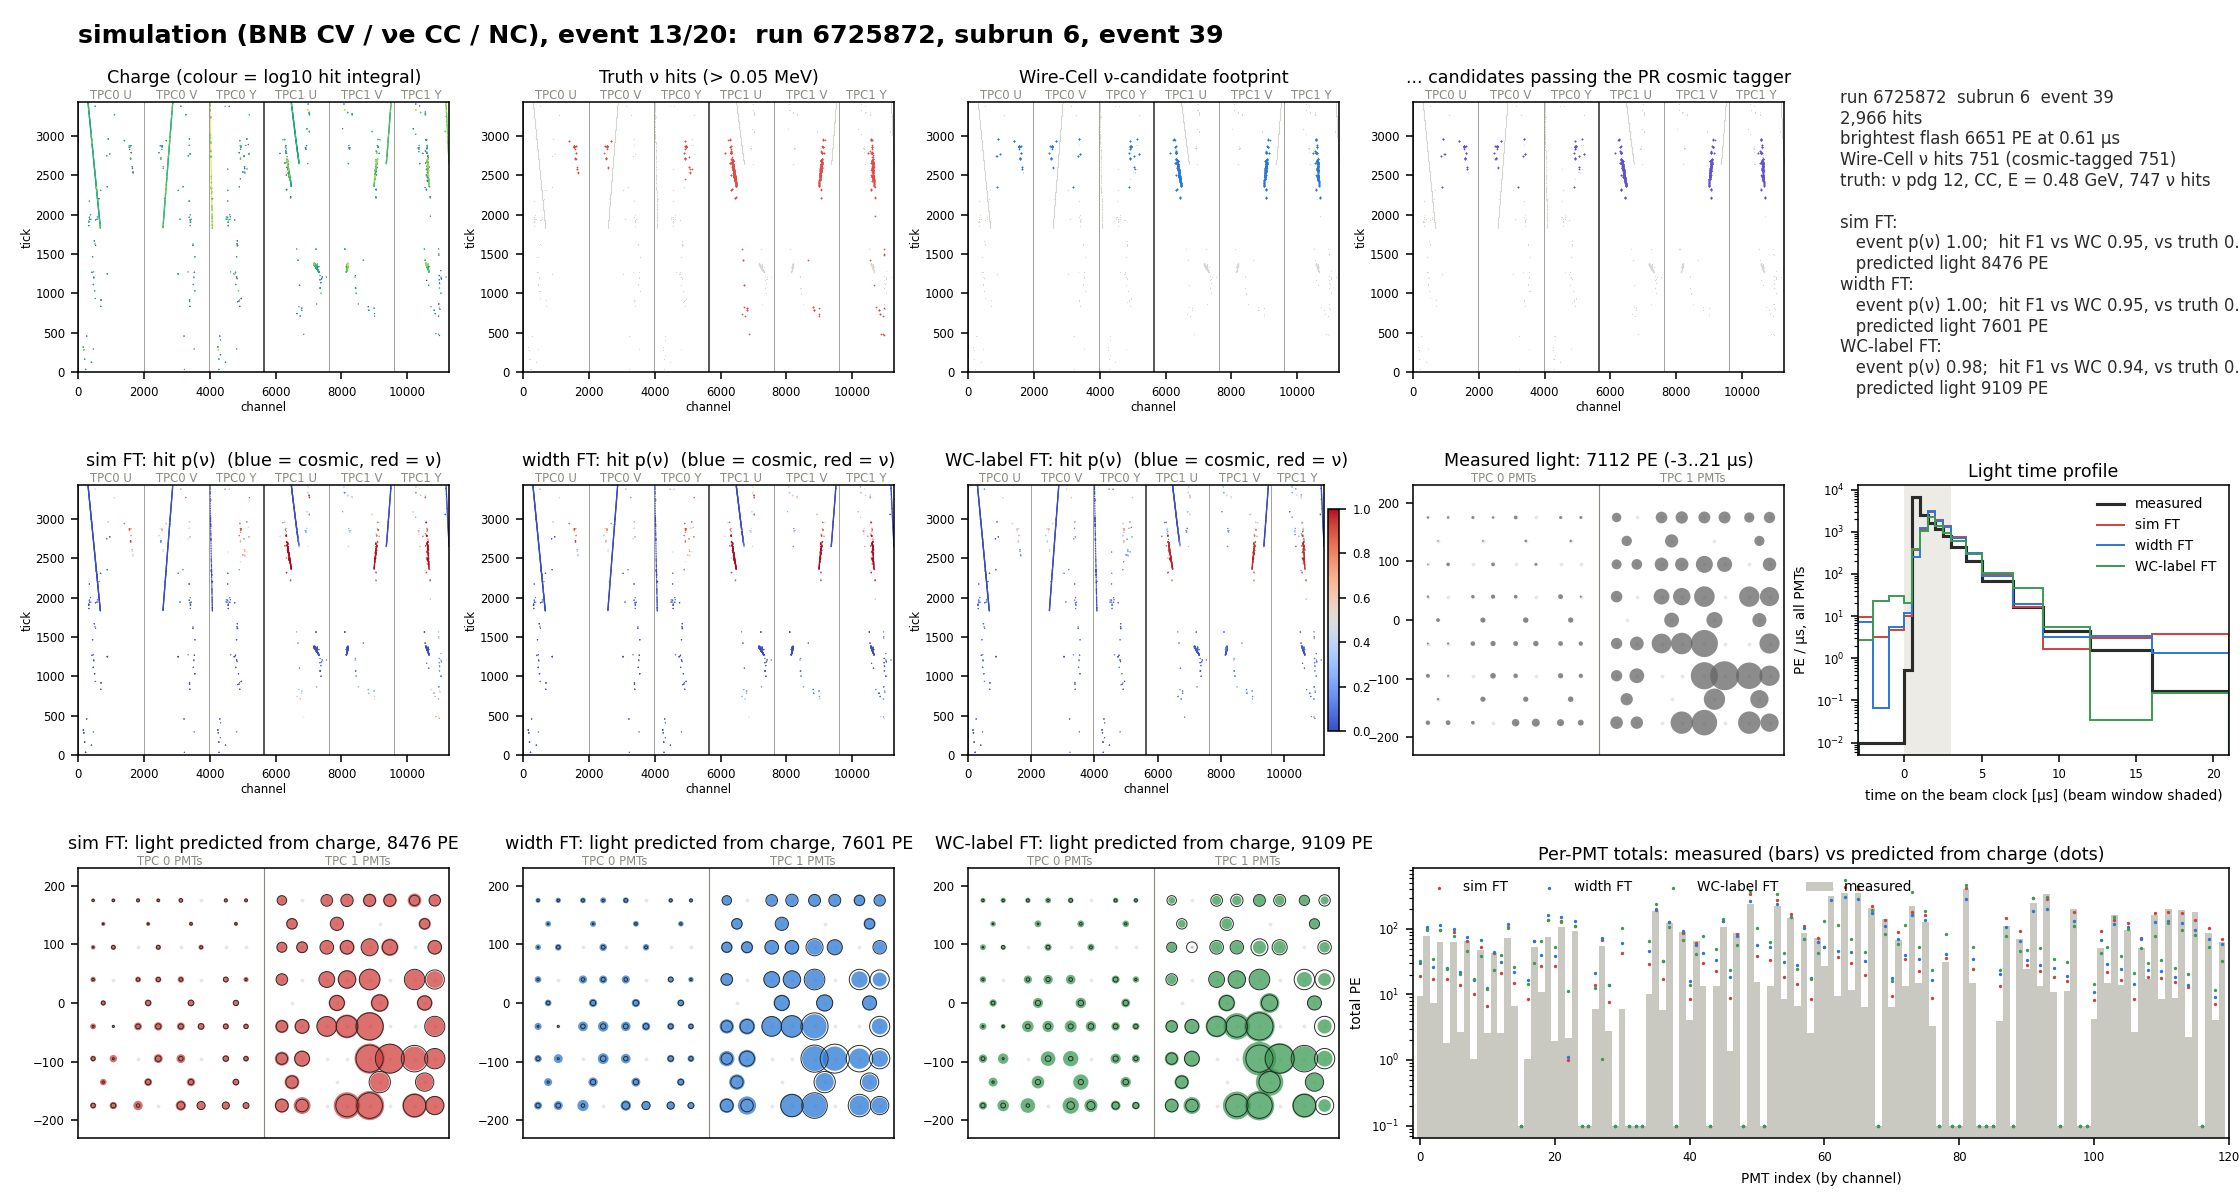
\includegraphics[width=\paperwidth,height=\paperheight,keepaspectratio]{displays/sim_12.jpg}}
\end{frame}
% Simulation 14/20: run 6731633, subrun 49, event 68; event p(nu): sim FT 1.00, width FT 1.00, WC-label FT 0.99
\begin{frame}[plain]
  \centering\vspace*{-2pt}
  \makebox[\linewidth][c]{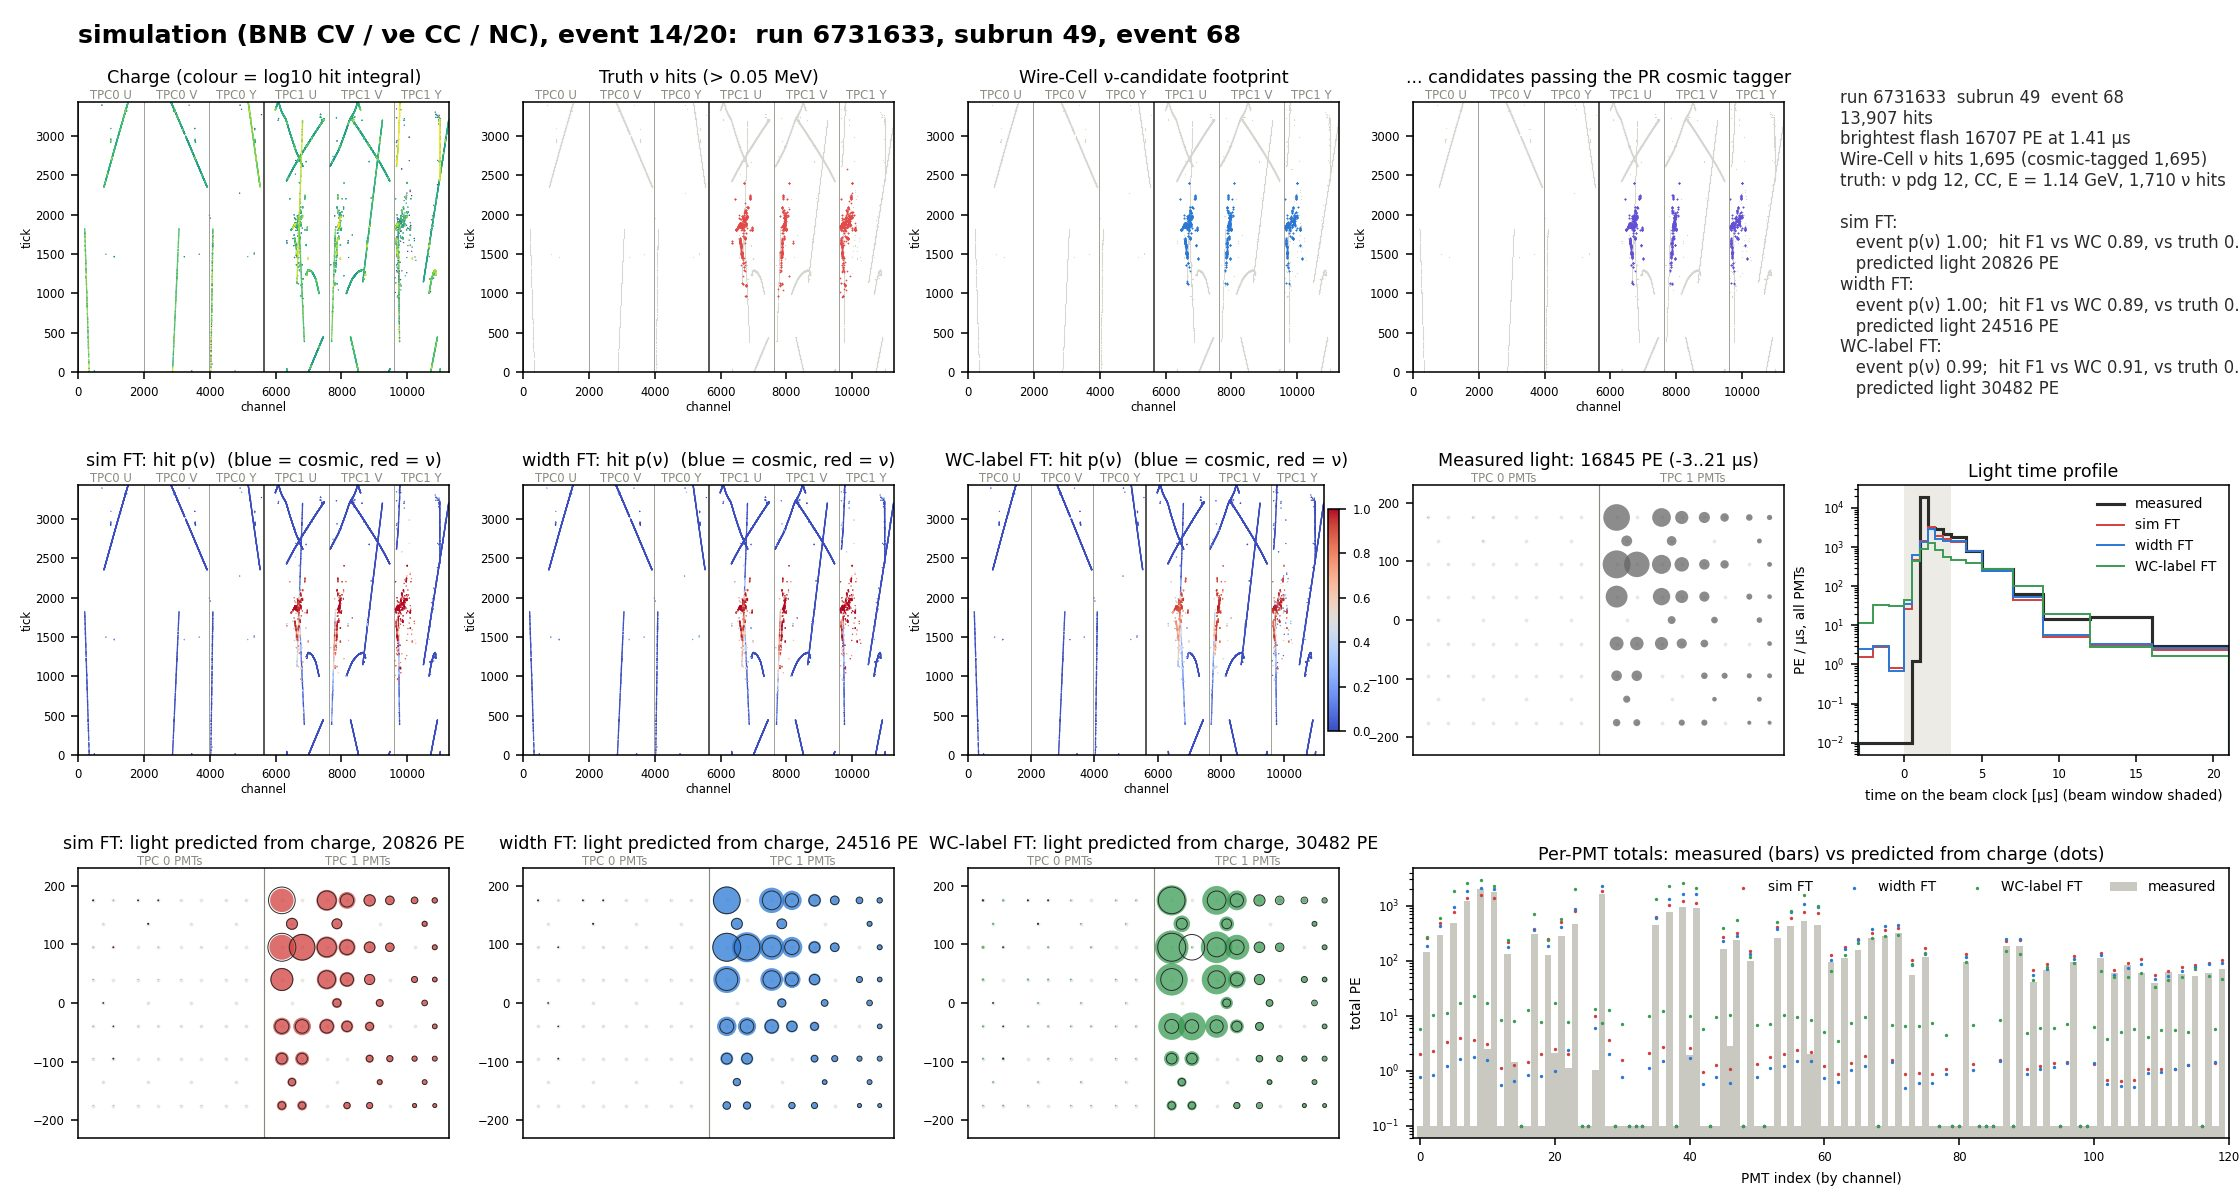
\includegraphics[width=\paperwidth,height=\paperheight,keepaspectratio]{displays/sim_13.jpg}}
\end{frame}
% Simulation 15/20: run 6701731, subrun 3, event 92; event p(nu): sim FT 1.00, width FT 1.00, WC-label FT 0.99
\begin{frame}[plain]
  \centering\vspace*{-2pt}
  \makebox[\linewidth][c]{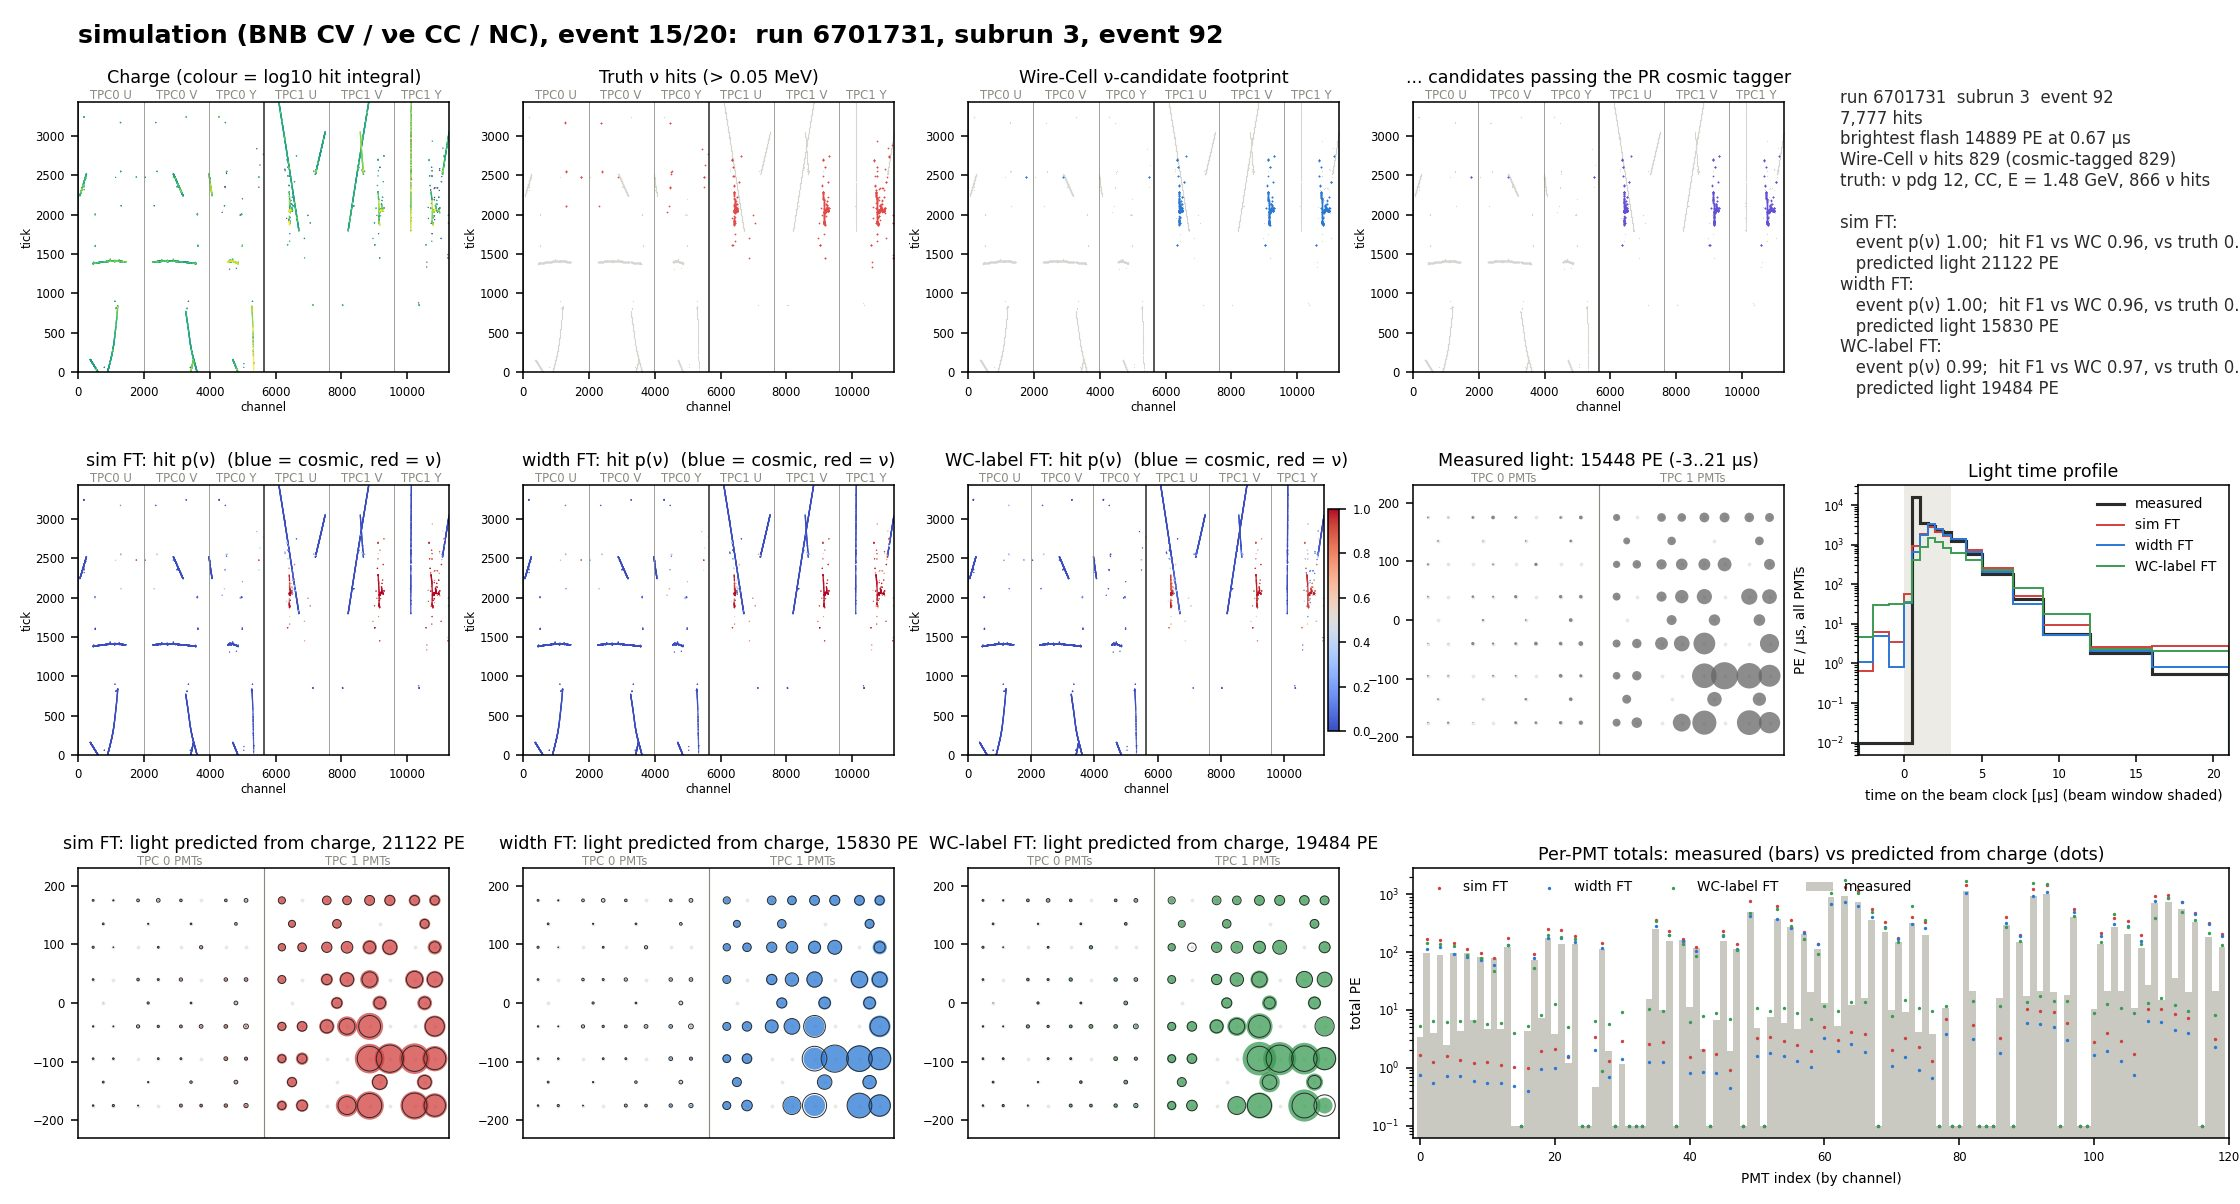
\includegraphics[width=\paperwidth,height=\paperheight,keepaspectratio]{displays/sim_14.jpg}}
\end{frame}
% Simulation 16/20: run 6712578, subrun 67, event 77; event p(nu): sim FT 1.00, width FT 1.00, WC-label FT 1.00
\begin{frame}[plain]
  \centering\vspace*{-2pt}
  \makebox[\linewidth][c]{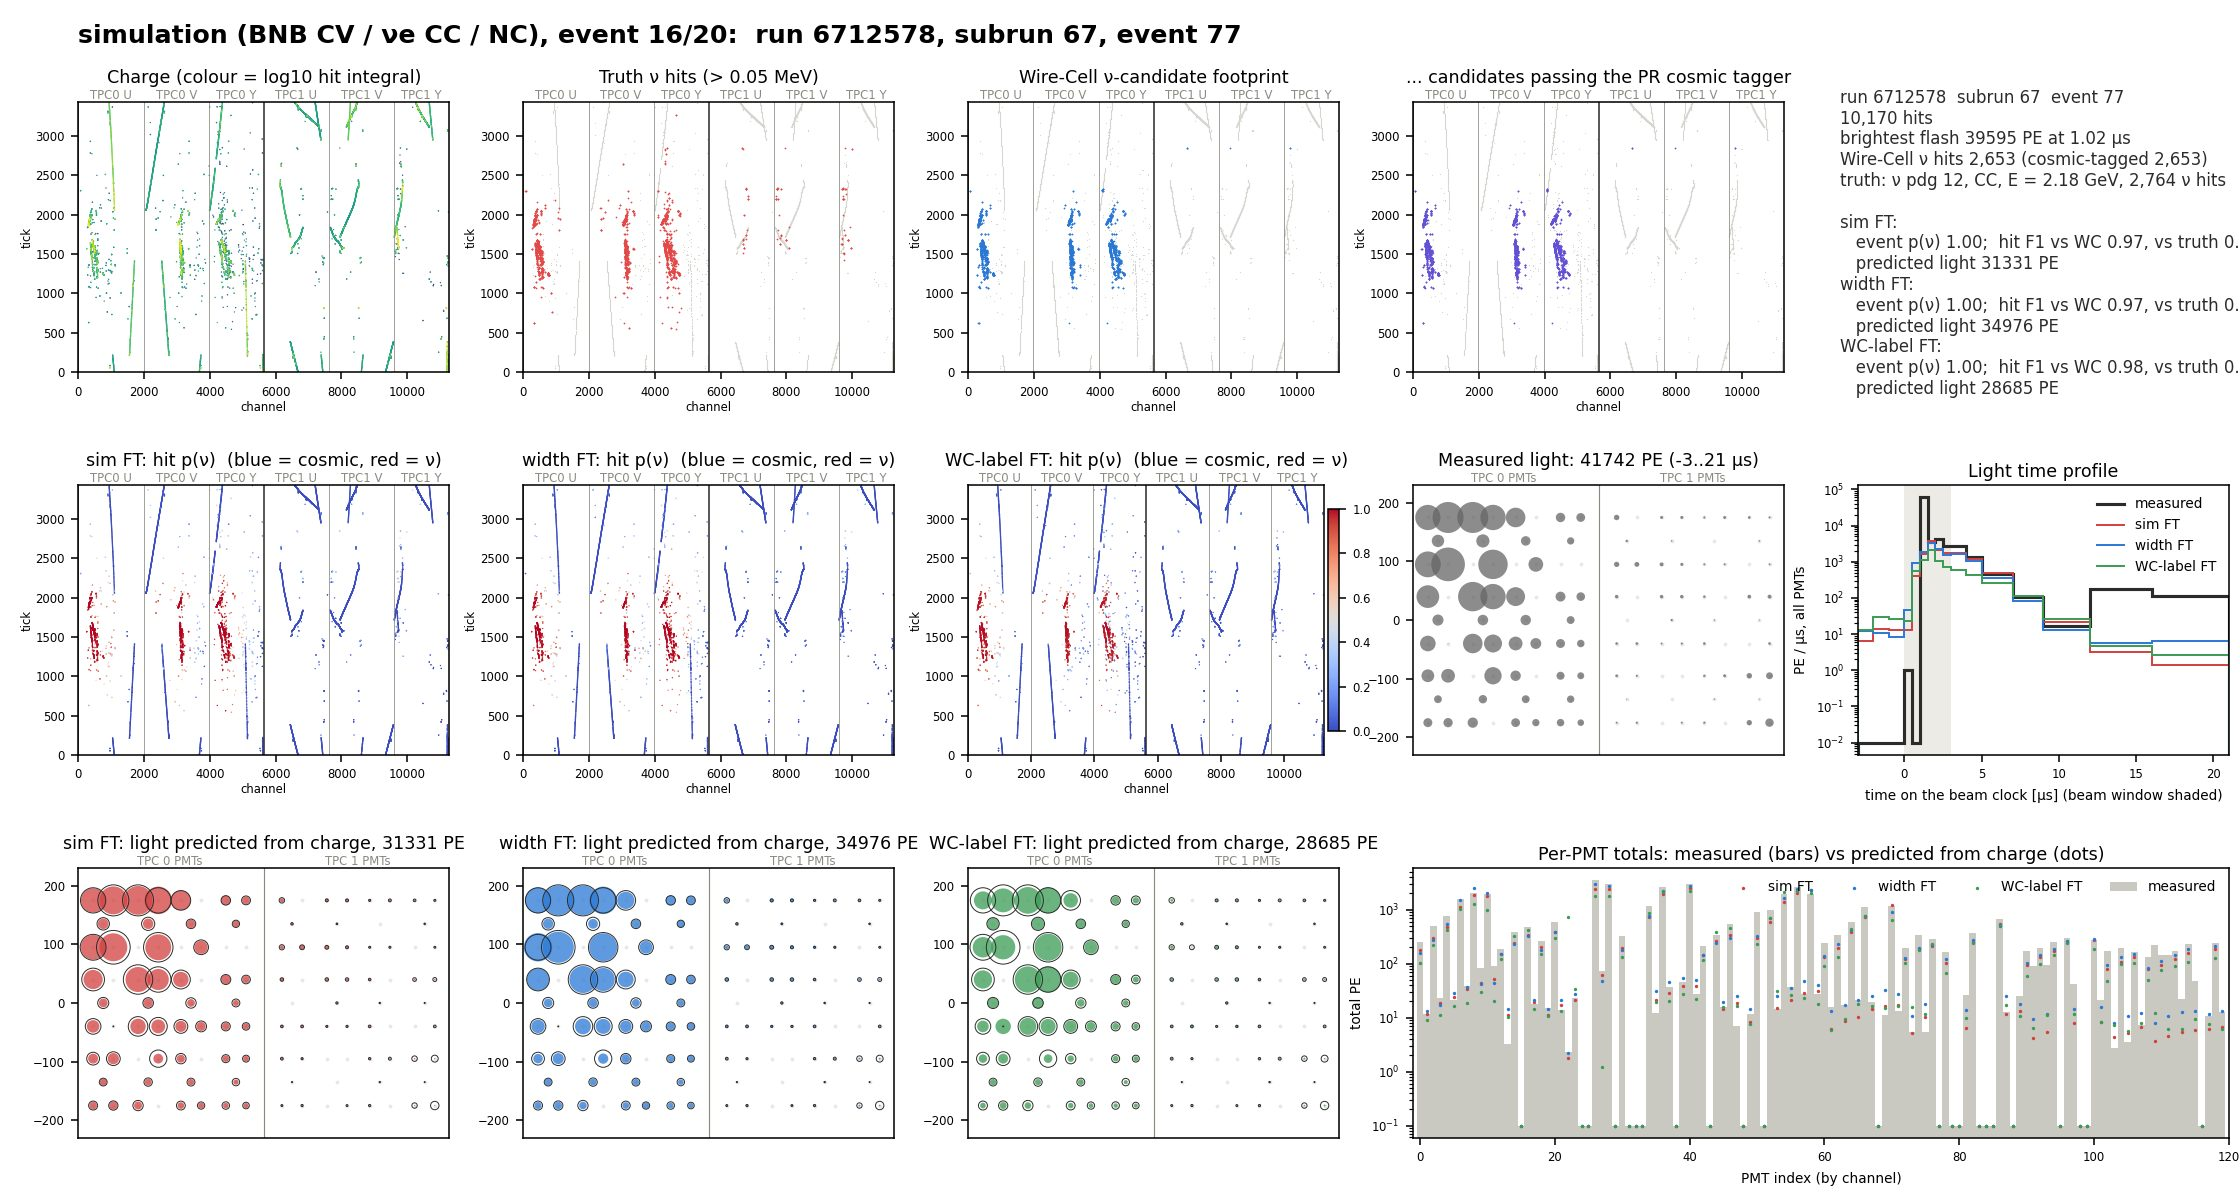
\includegraphics[width=\paperwidth,height=\paperheight,keepaspectratio]{displays/sim_15.jpg}}
\end{frame}
% Simulation 17/20: run 6714530, subrun 46, event 93; event p(nu): sim FT 1.00, width FT 1.00, WC-label FT 0.99
\begin{frame}[plain]
  \centering\vspace*{-2pt}
  \makebox[\linewidth][c]{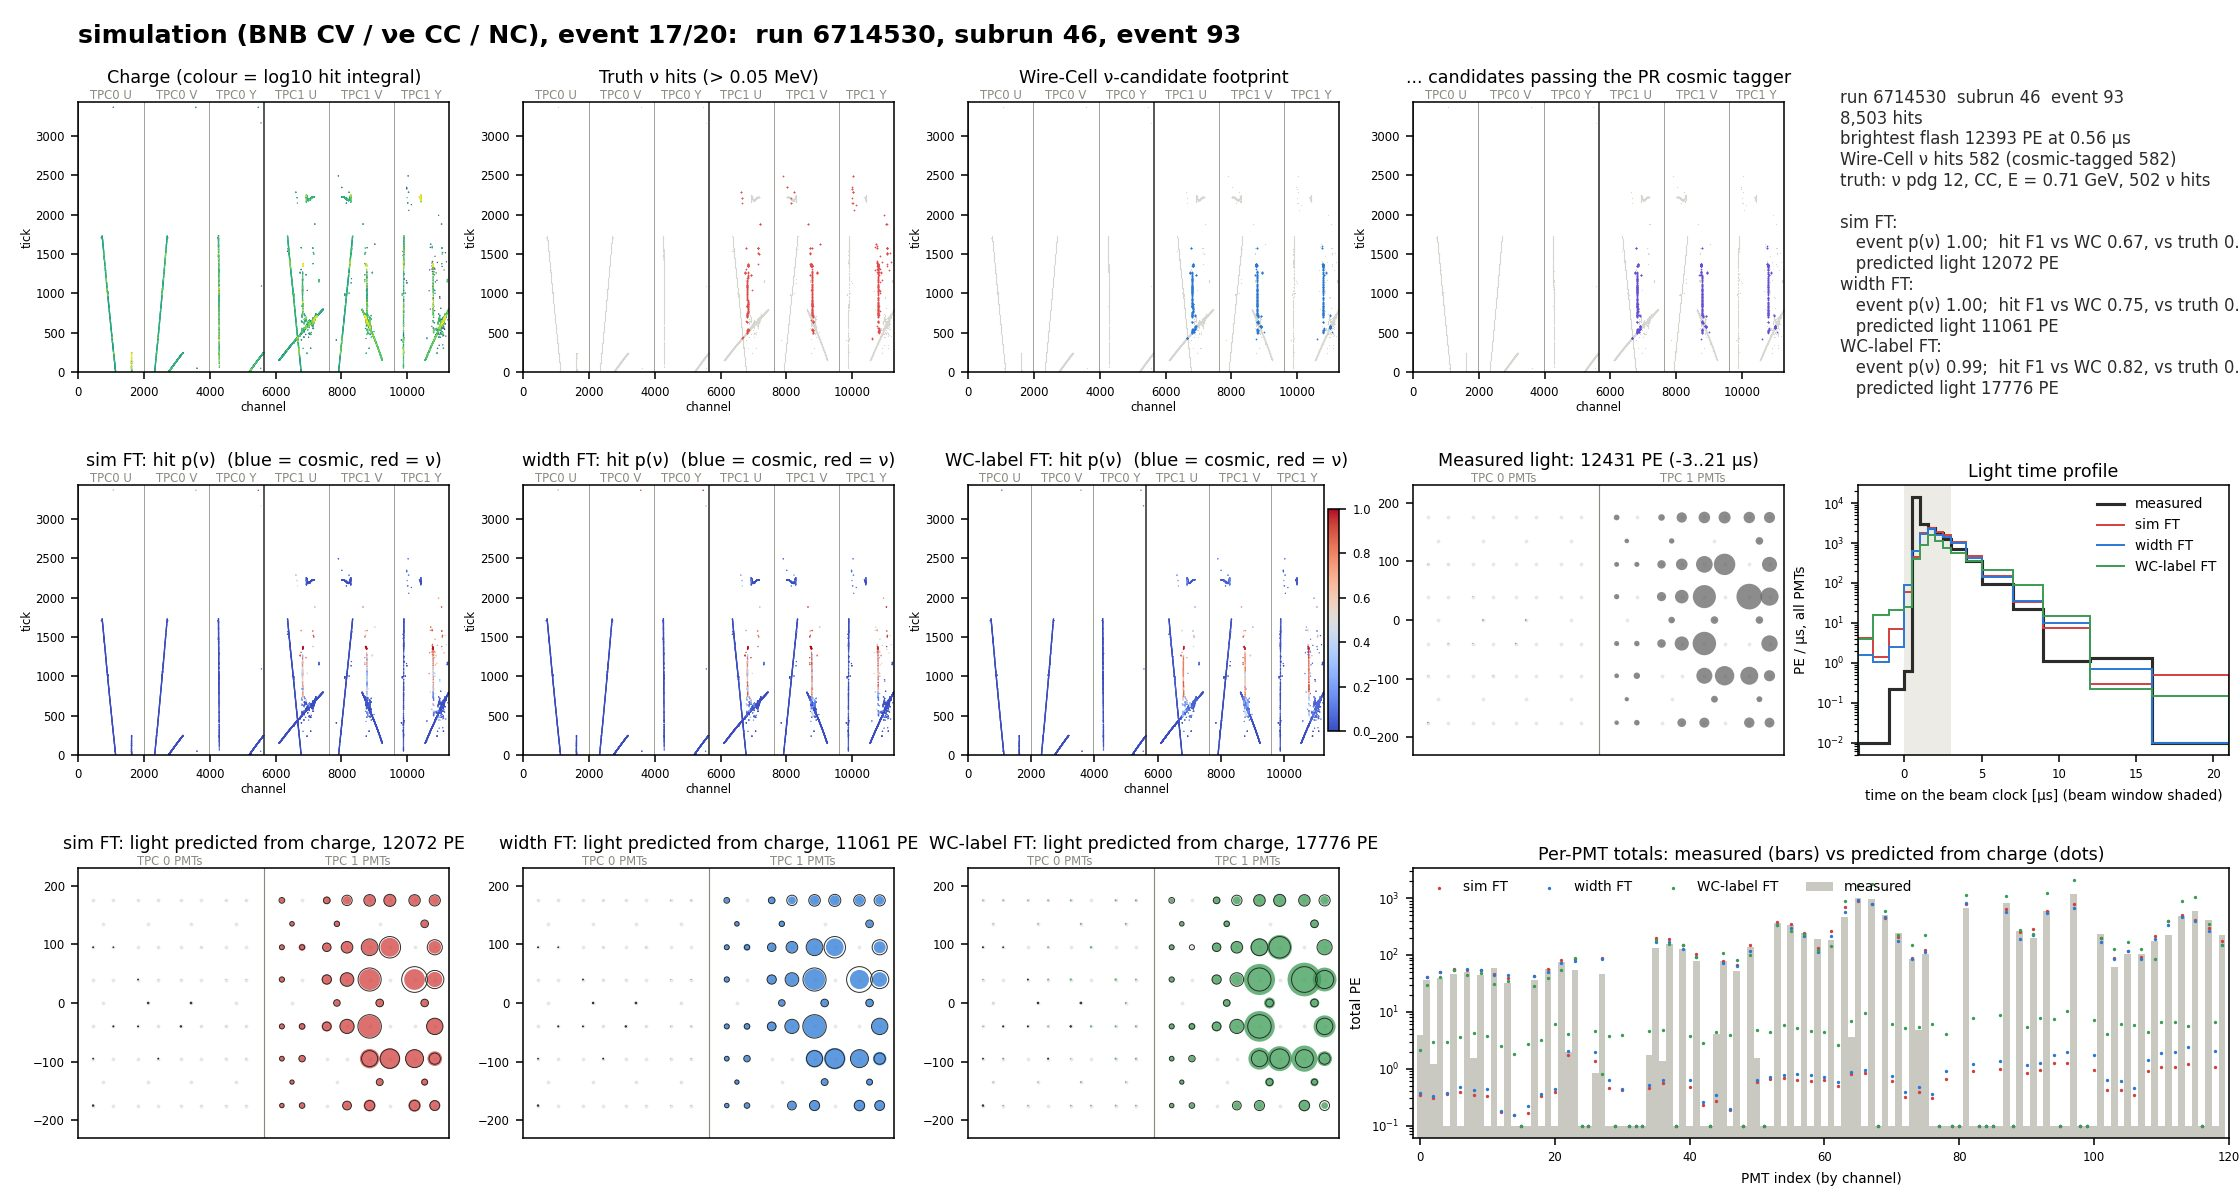
\includegraphics[width=\paperwidth,height=\paperheight,keepaspectratio]{displays/sim_16.jpg}}
\end{frame}
% Simulation 18/20: run 6712567, subrun 38, event 15; event p(nu): sim FT 1.00, width FT 1.00, WC-label FT 0.99
\begin{frame}[plain]
  \centering\vspace*{-2pt}
  \makebox[\linewidth][c]{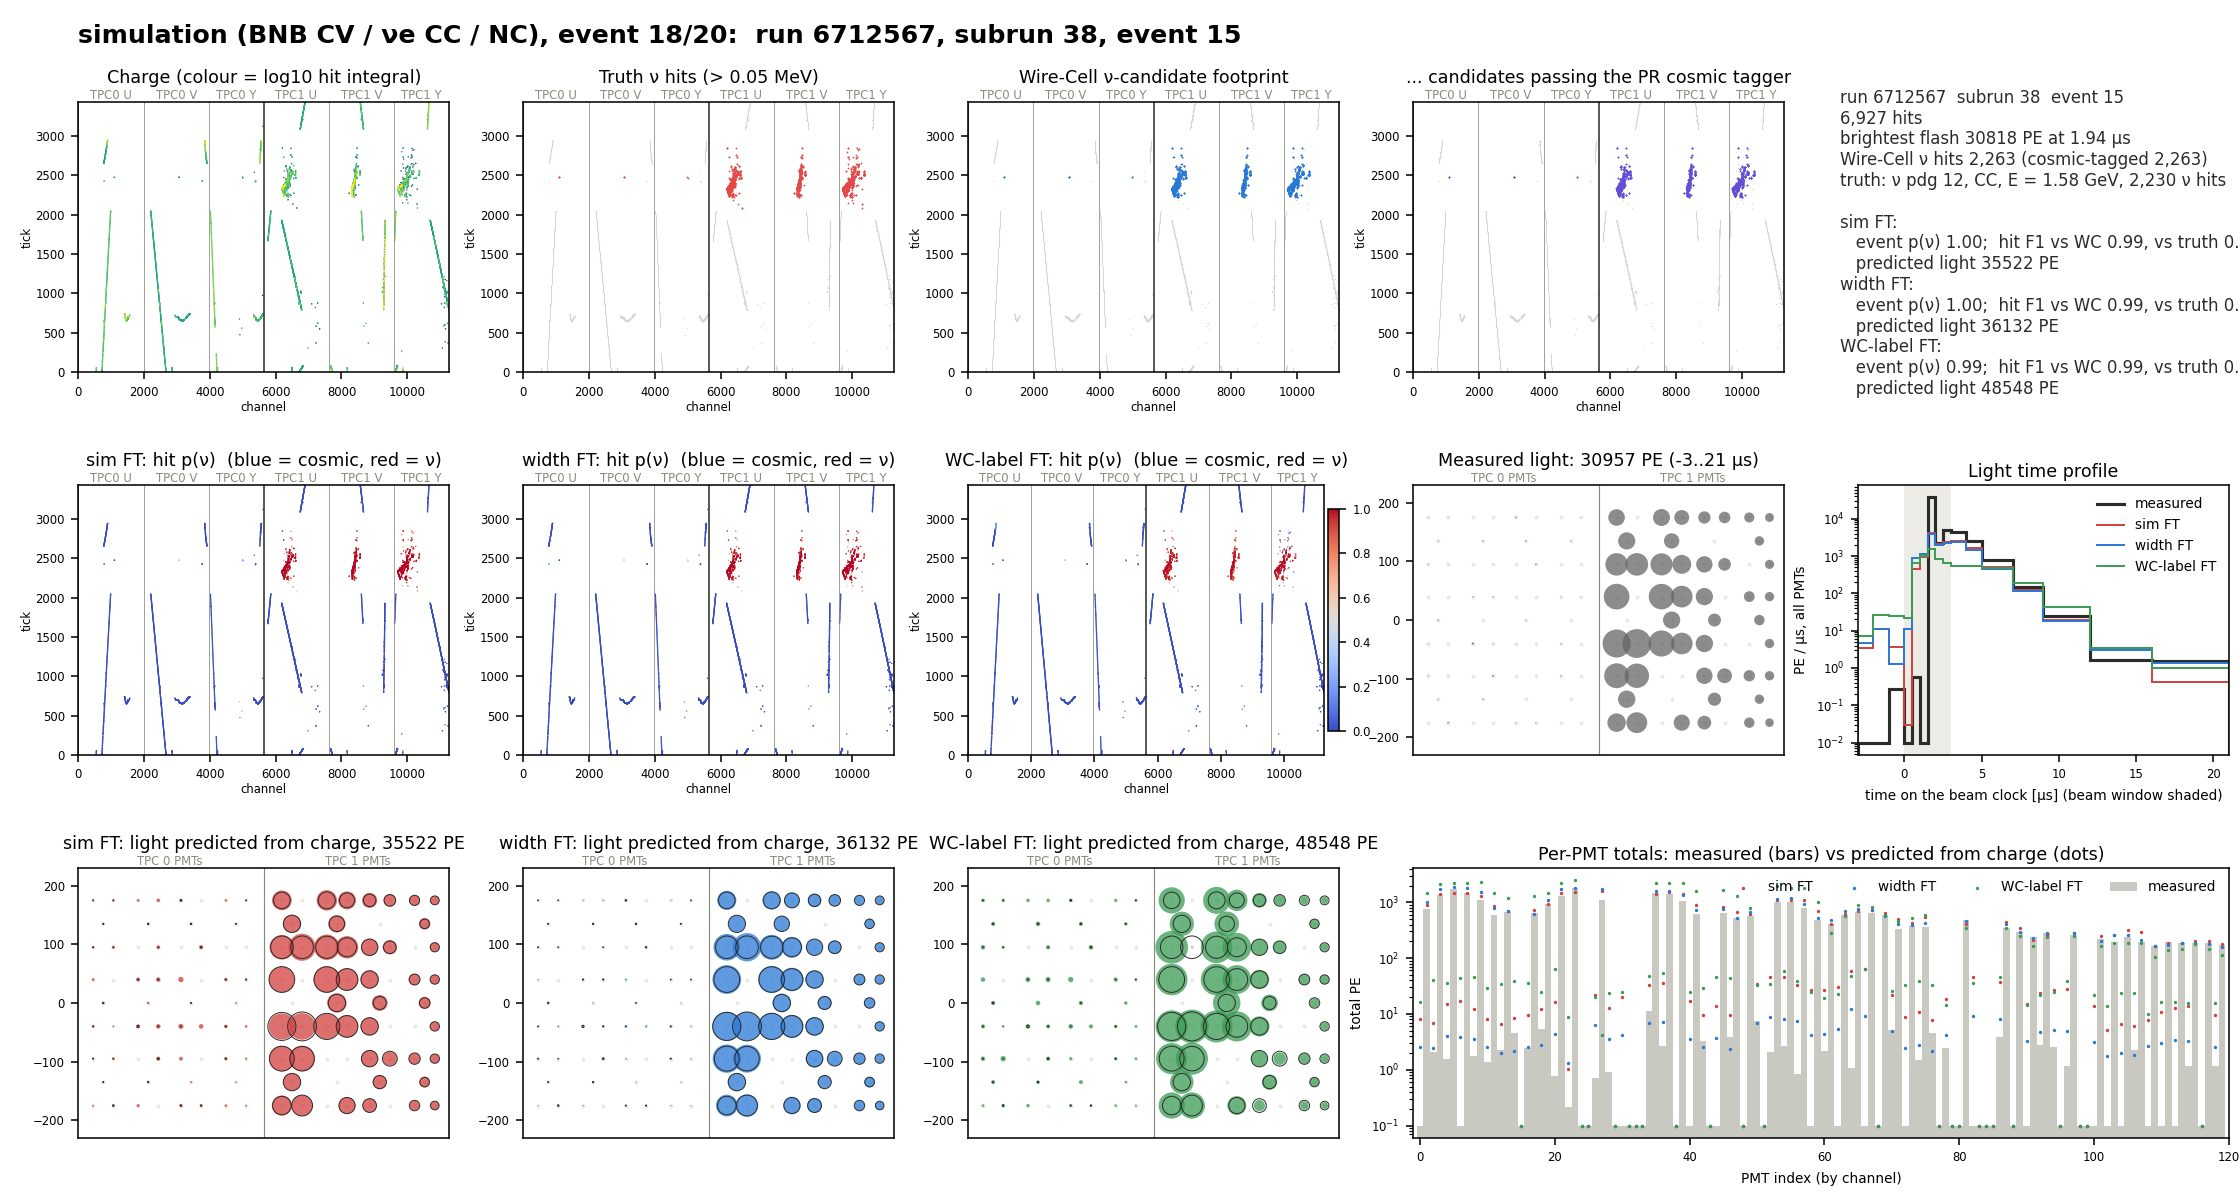
\includegraphics[width=\paperwidth,height=\paperheight,keepaspectratio]{displays/sim_17.jpg}}
\end{frame}
% Simulation 19/20: run 6703266, subrun 87, event 83; event p(nu): sim FT 0.74, width FT 0.51, WC-label FT 0.99
\begin{frame}[plain]
  \centering\vspace*{-2pt}
  \makebox[\linewidth][c]{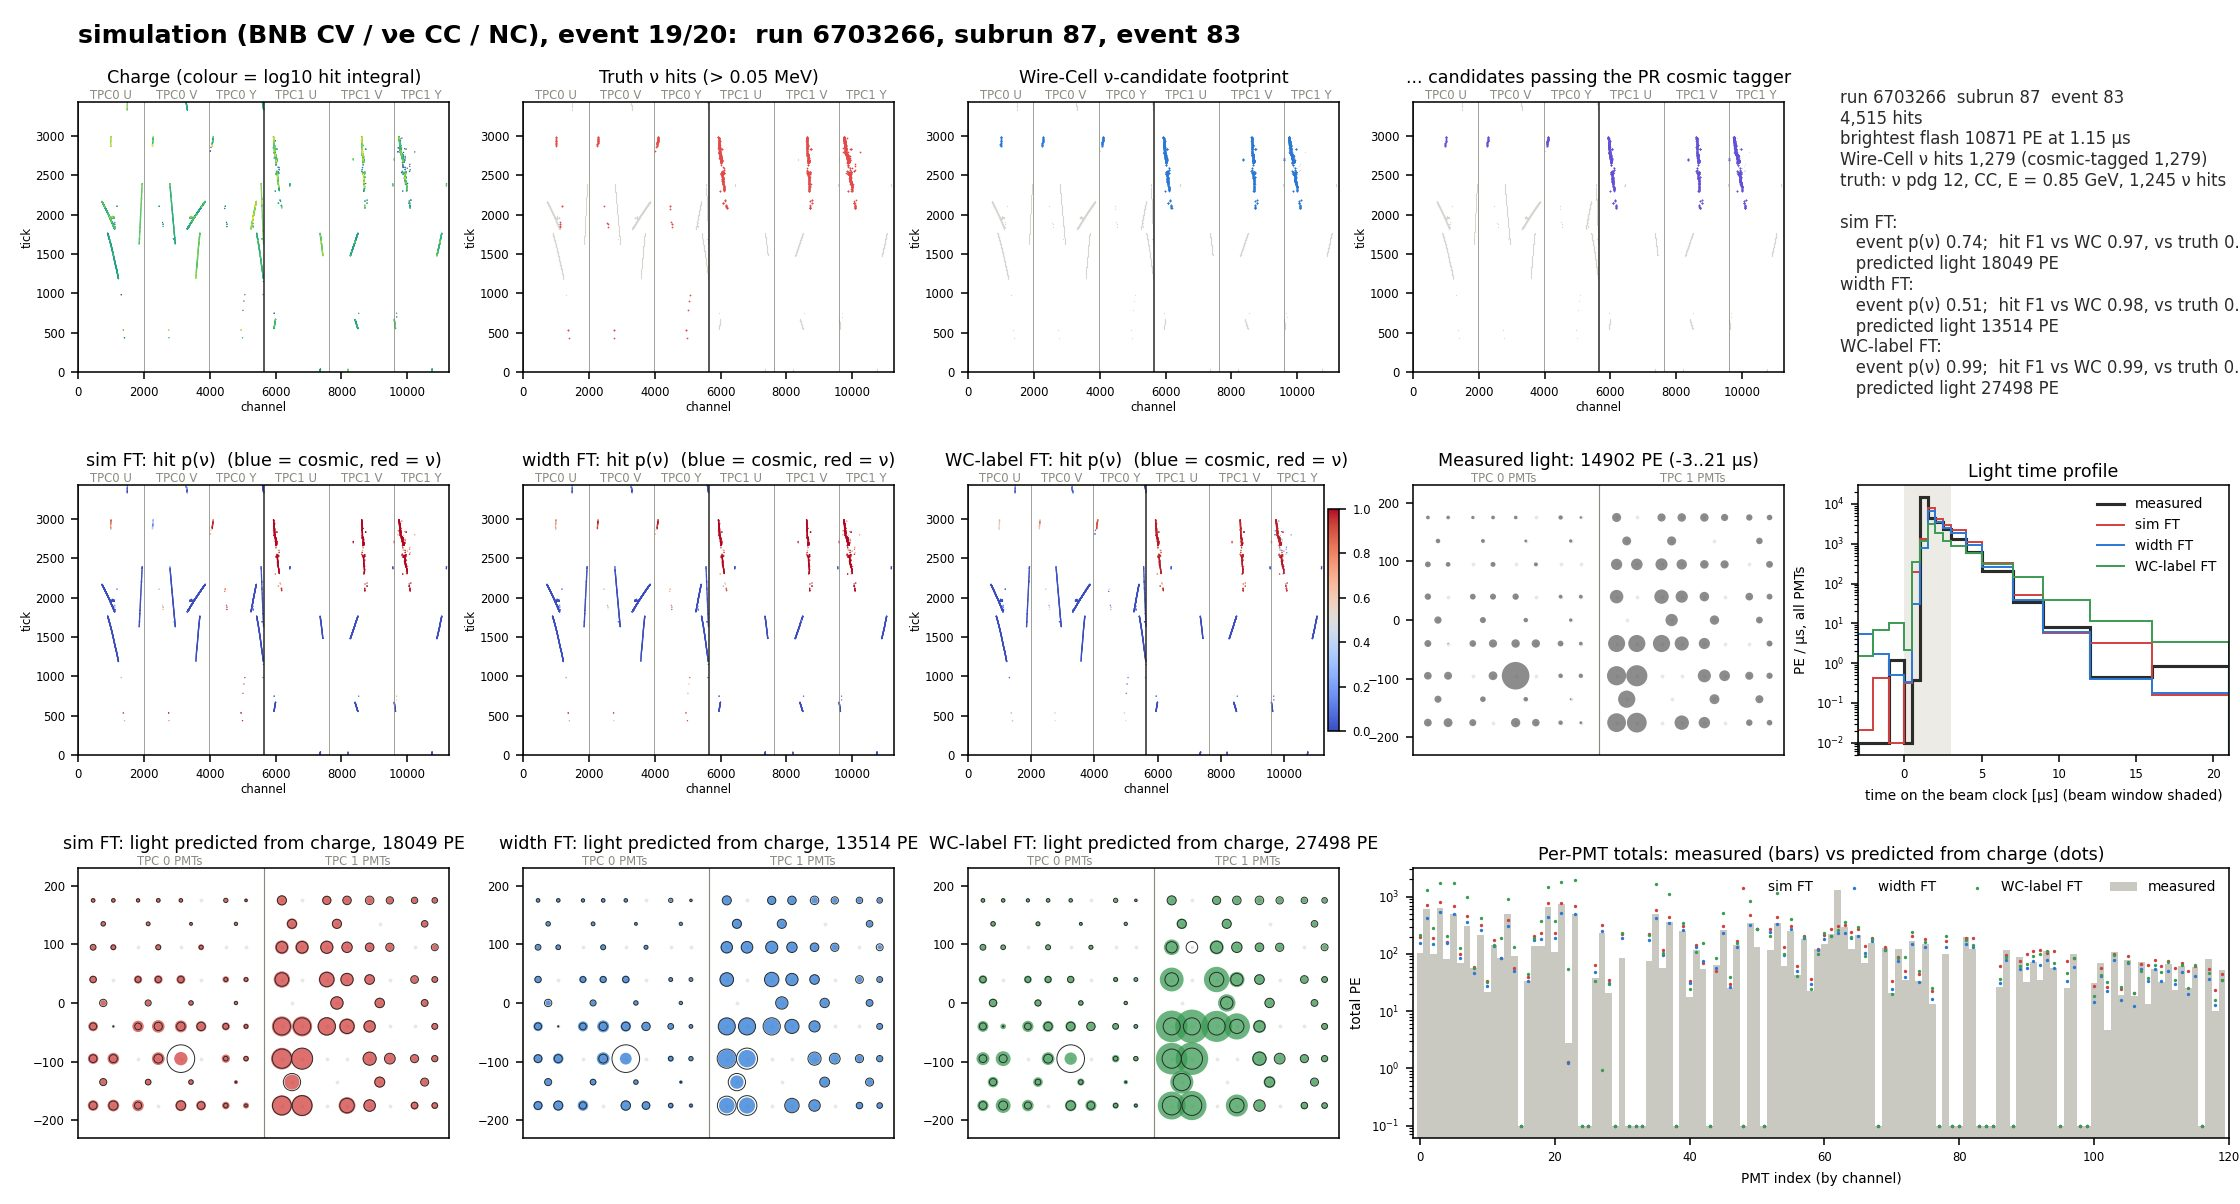
\includegraphics[width=\paperwidth,height=\paperheight,keepaspectratio]{displays/sim_18.jpg}}
\end{frame}
% Simulation 20/20: run 7022028, subrun 0, event 121; event p(nu): sim FT 1.00, width FT 1.00, WC-label FT 0.81
\begin{frame}[plain]
  \centering\vspace*{-2pt}
  \makebox[\linewidth][c]{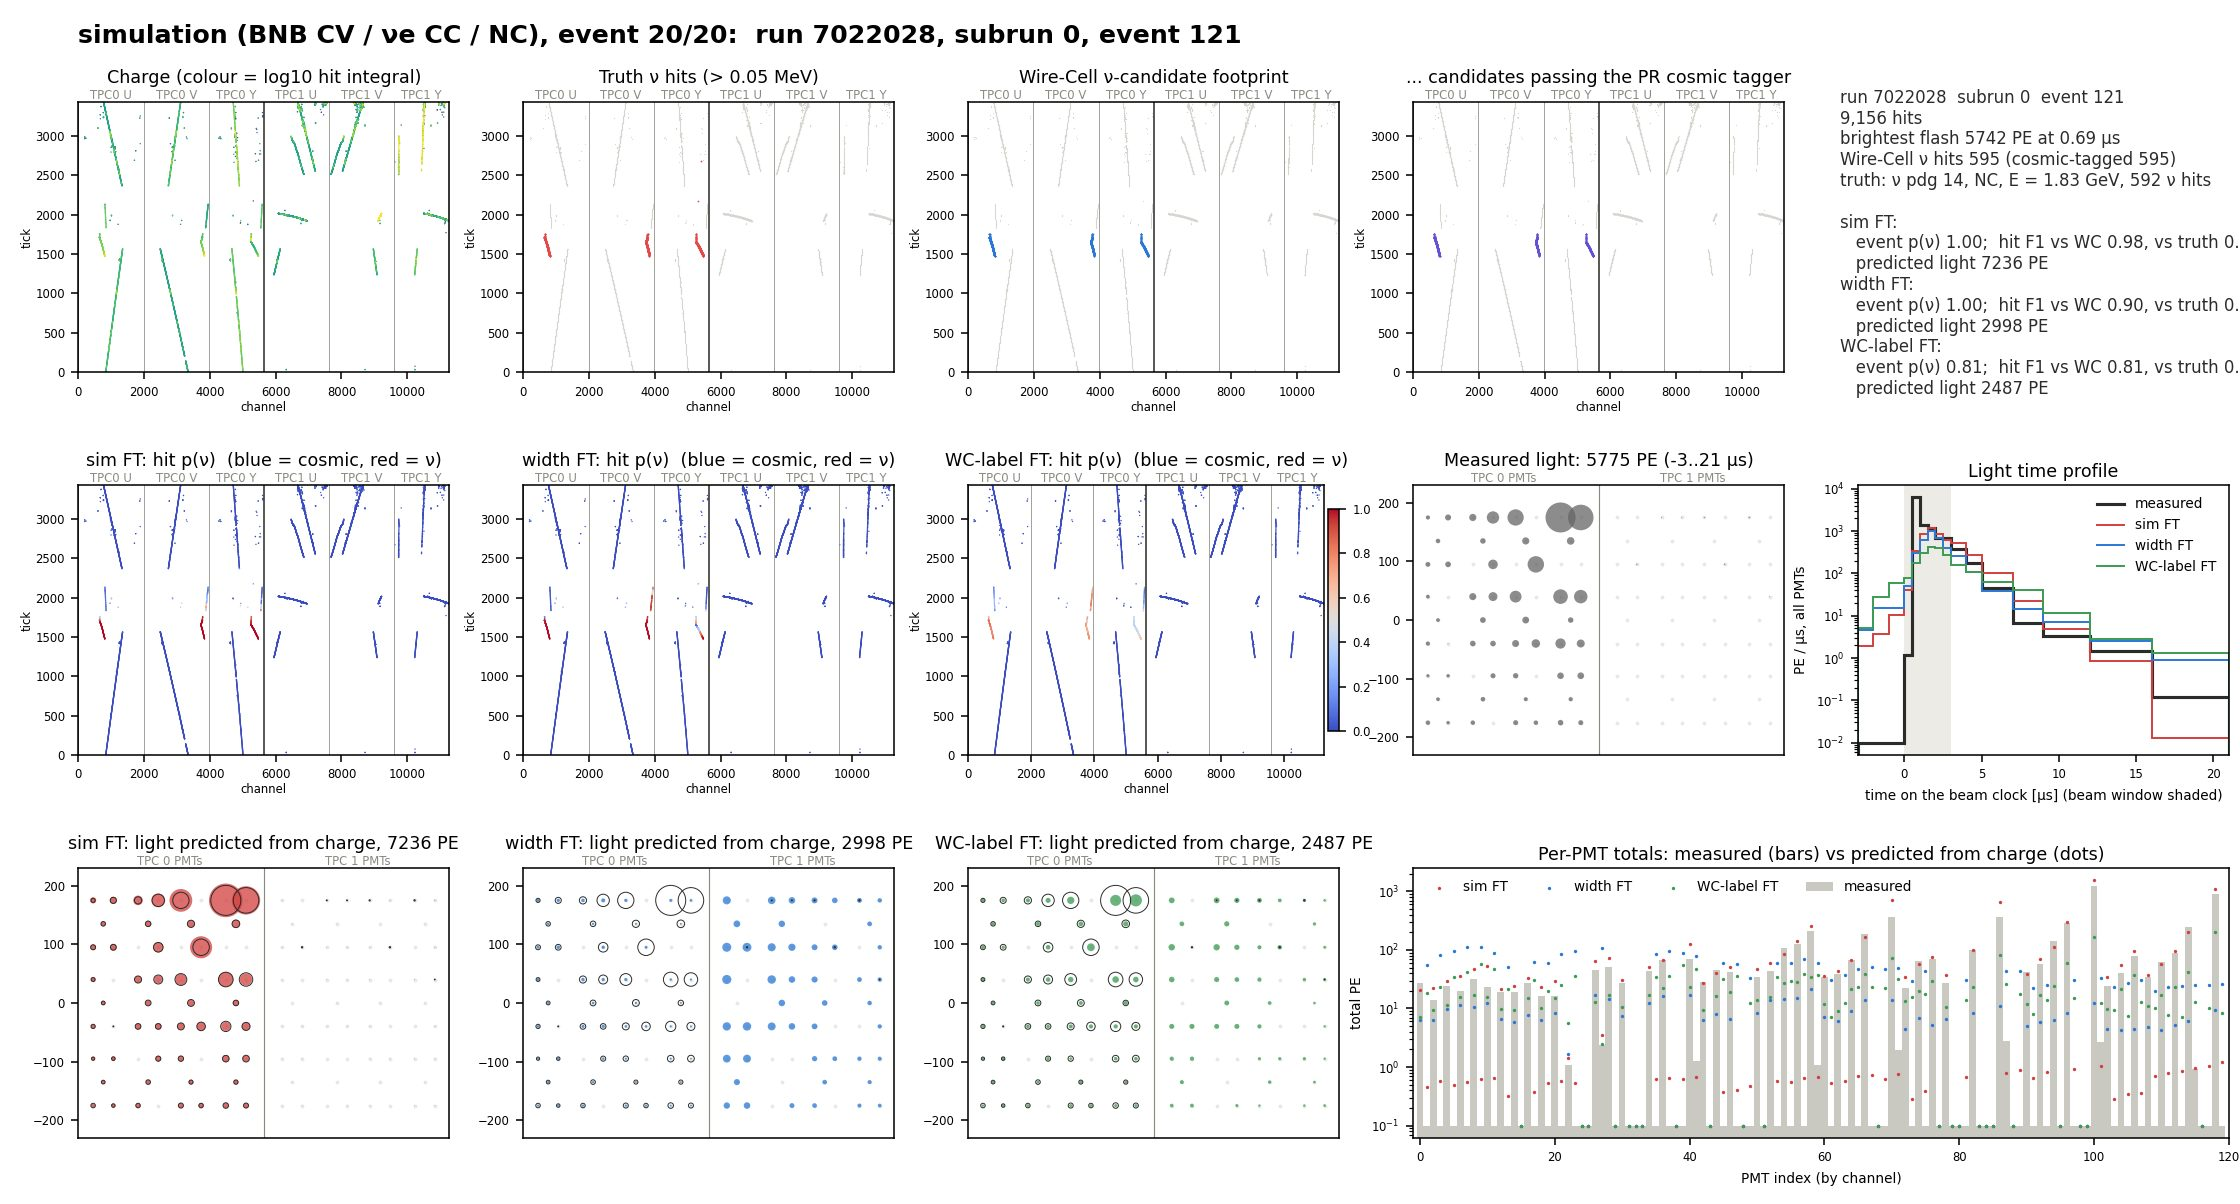
\includegraphics[width=\paperwidth,height=\paperheight,keepaspectratio]{displays/sim_19.jpg}}
\end{frame}
\subsection{Beam-on data}
% Beam-on data 1/20: run 18255, subrun 1, event 212212; event p(nu): sim FT 0.00, width FT 0.00, WC-label FT 0.00
\begin{frame}[plain]
  \centering\vspace*{-2pt}
  \makebox[\linewidth][c]{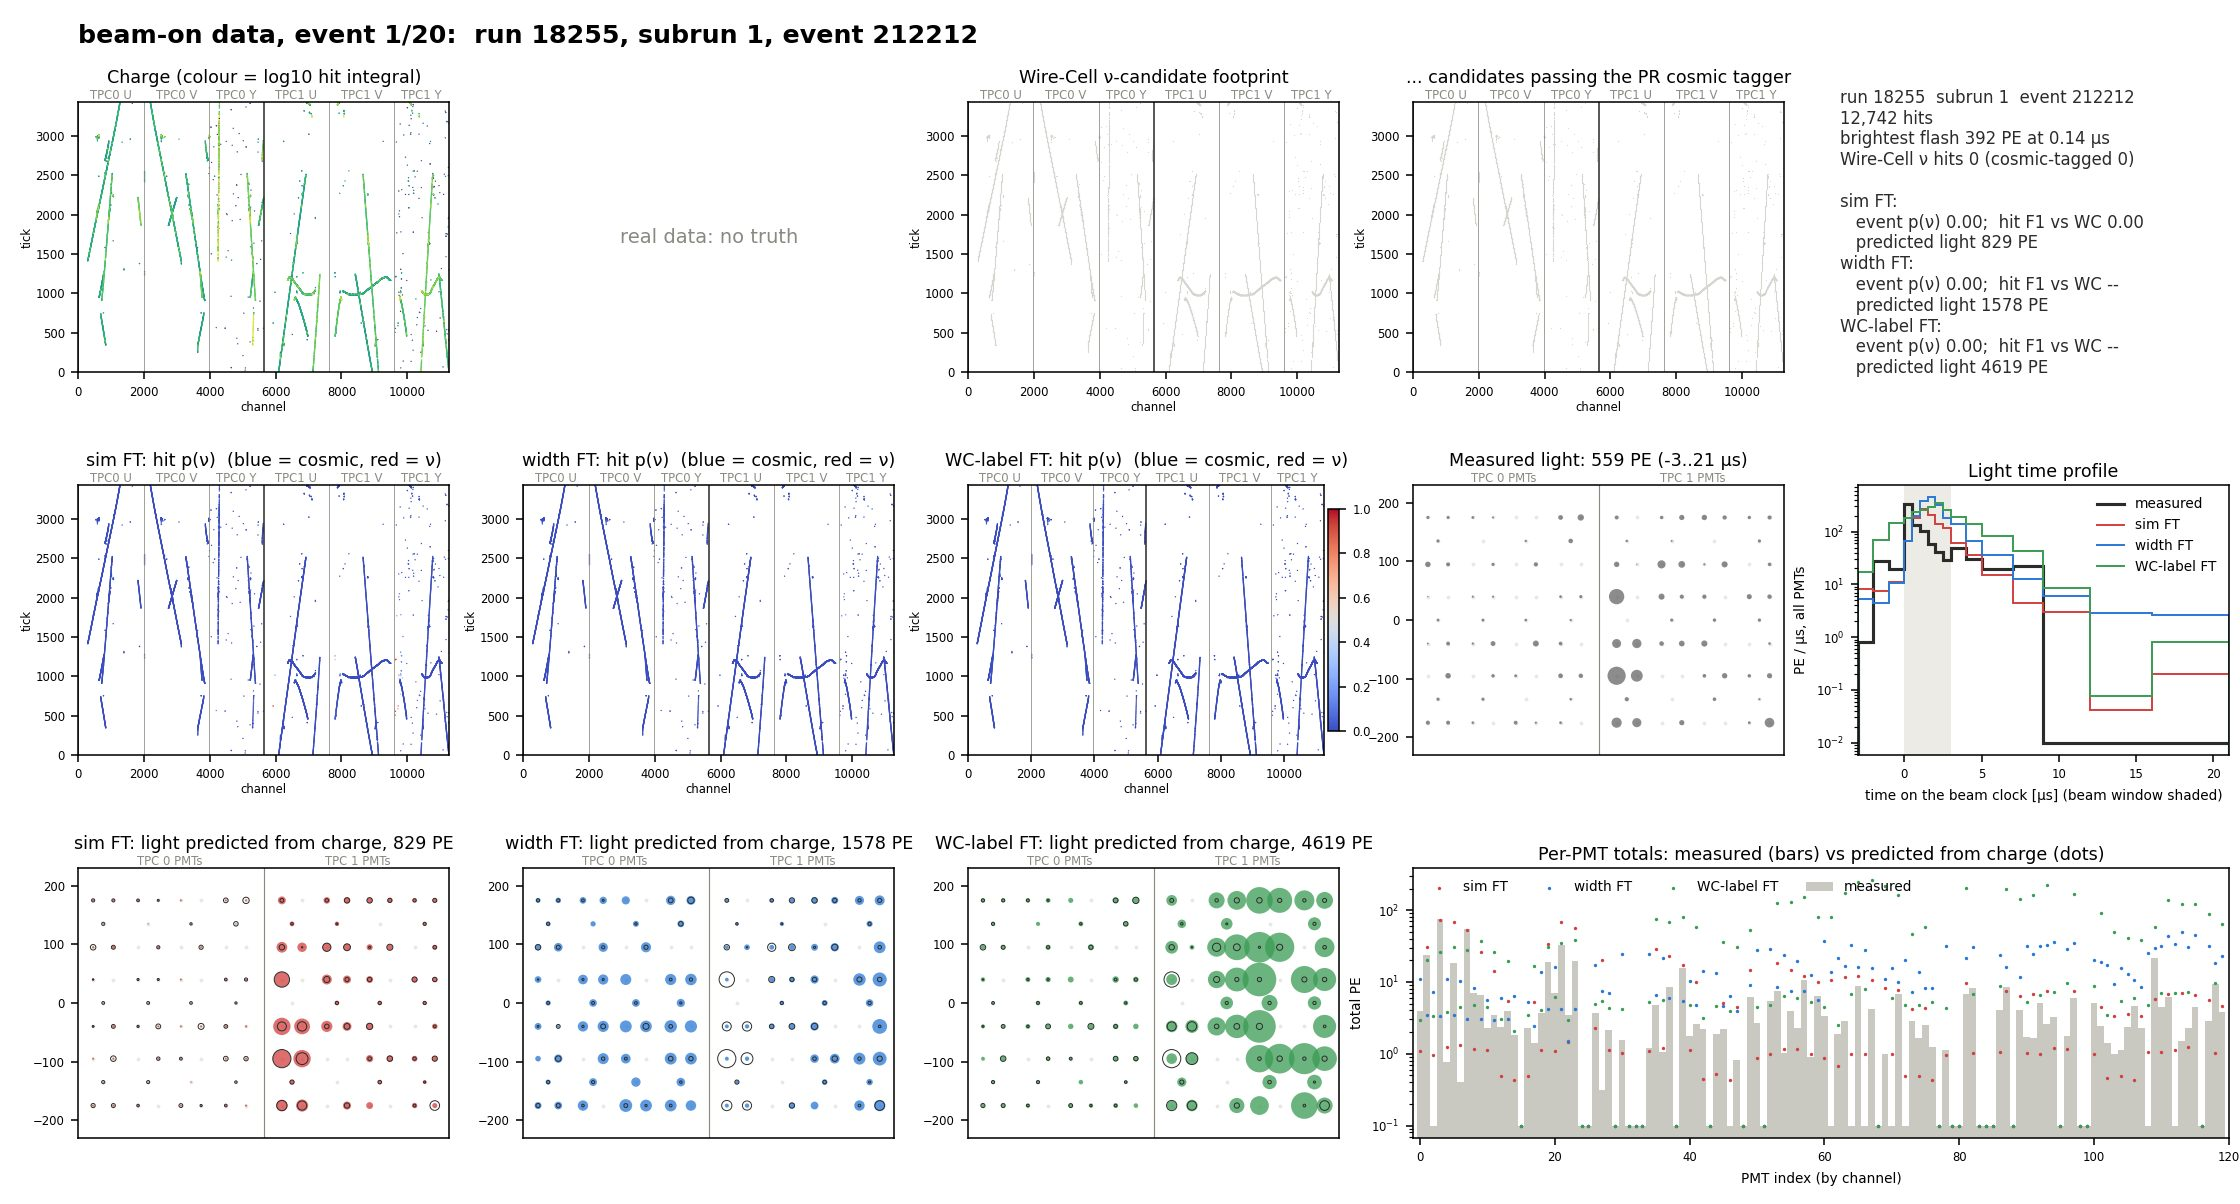
\includegraphics[width=\paperwidth,height=\paperheight,keepaspectratio]{displays/on_00.jpg}}
\end{frame}
% Beam-on data 2/20: run 18255, subrun 1, event 104444; event p(nu): sim FT 0.00, width FT 0.00, WC-label FT 0.90
\begin{frame}[plain]
  \centering\vspace*{-2pt}
  \makebox[\linewidth][c]{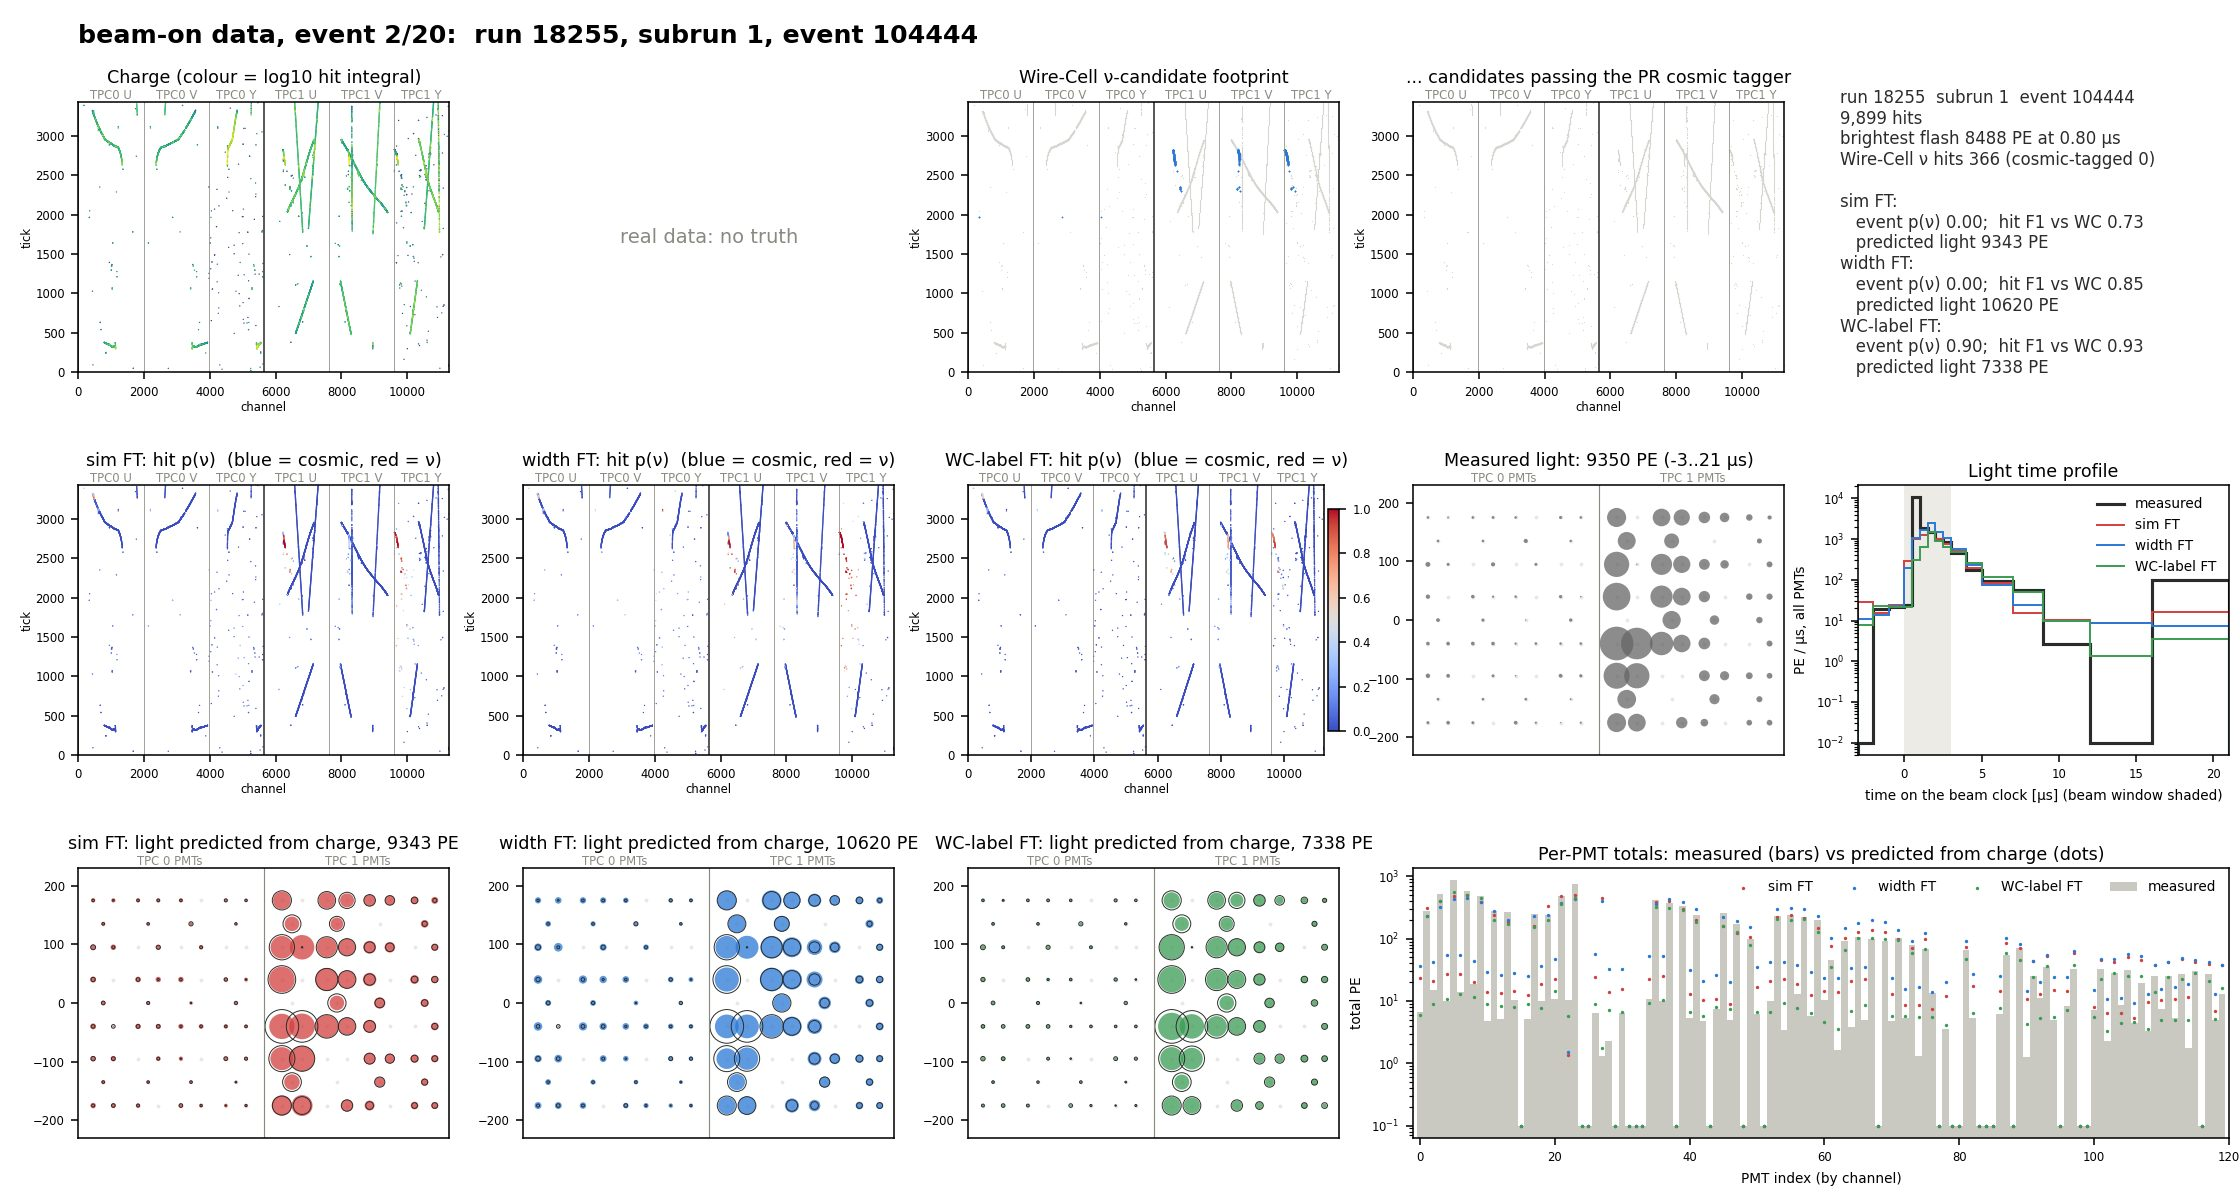
\includegraphics[width=\paperwidth,height=\paperheight,keepaspectratio]{displays/on_01.jpg}}
\end{frame}
% Beam-on data 3/20: run 18255, subrun 1, event 225882; event p(nu): sim FT 0.00, width FT 0.00, WC-label FT 0.34
\begin{frame}[plain]
  \centering\vspace*{-2pt}
  \makebox[\linewidth][c]{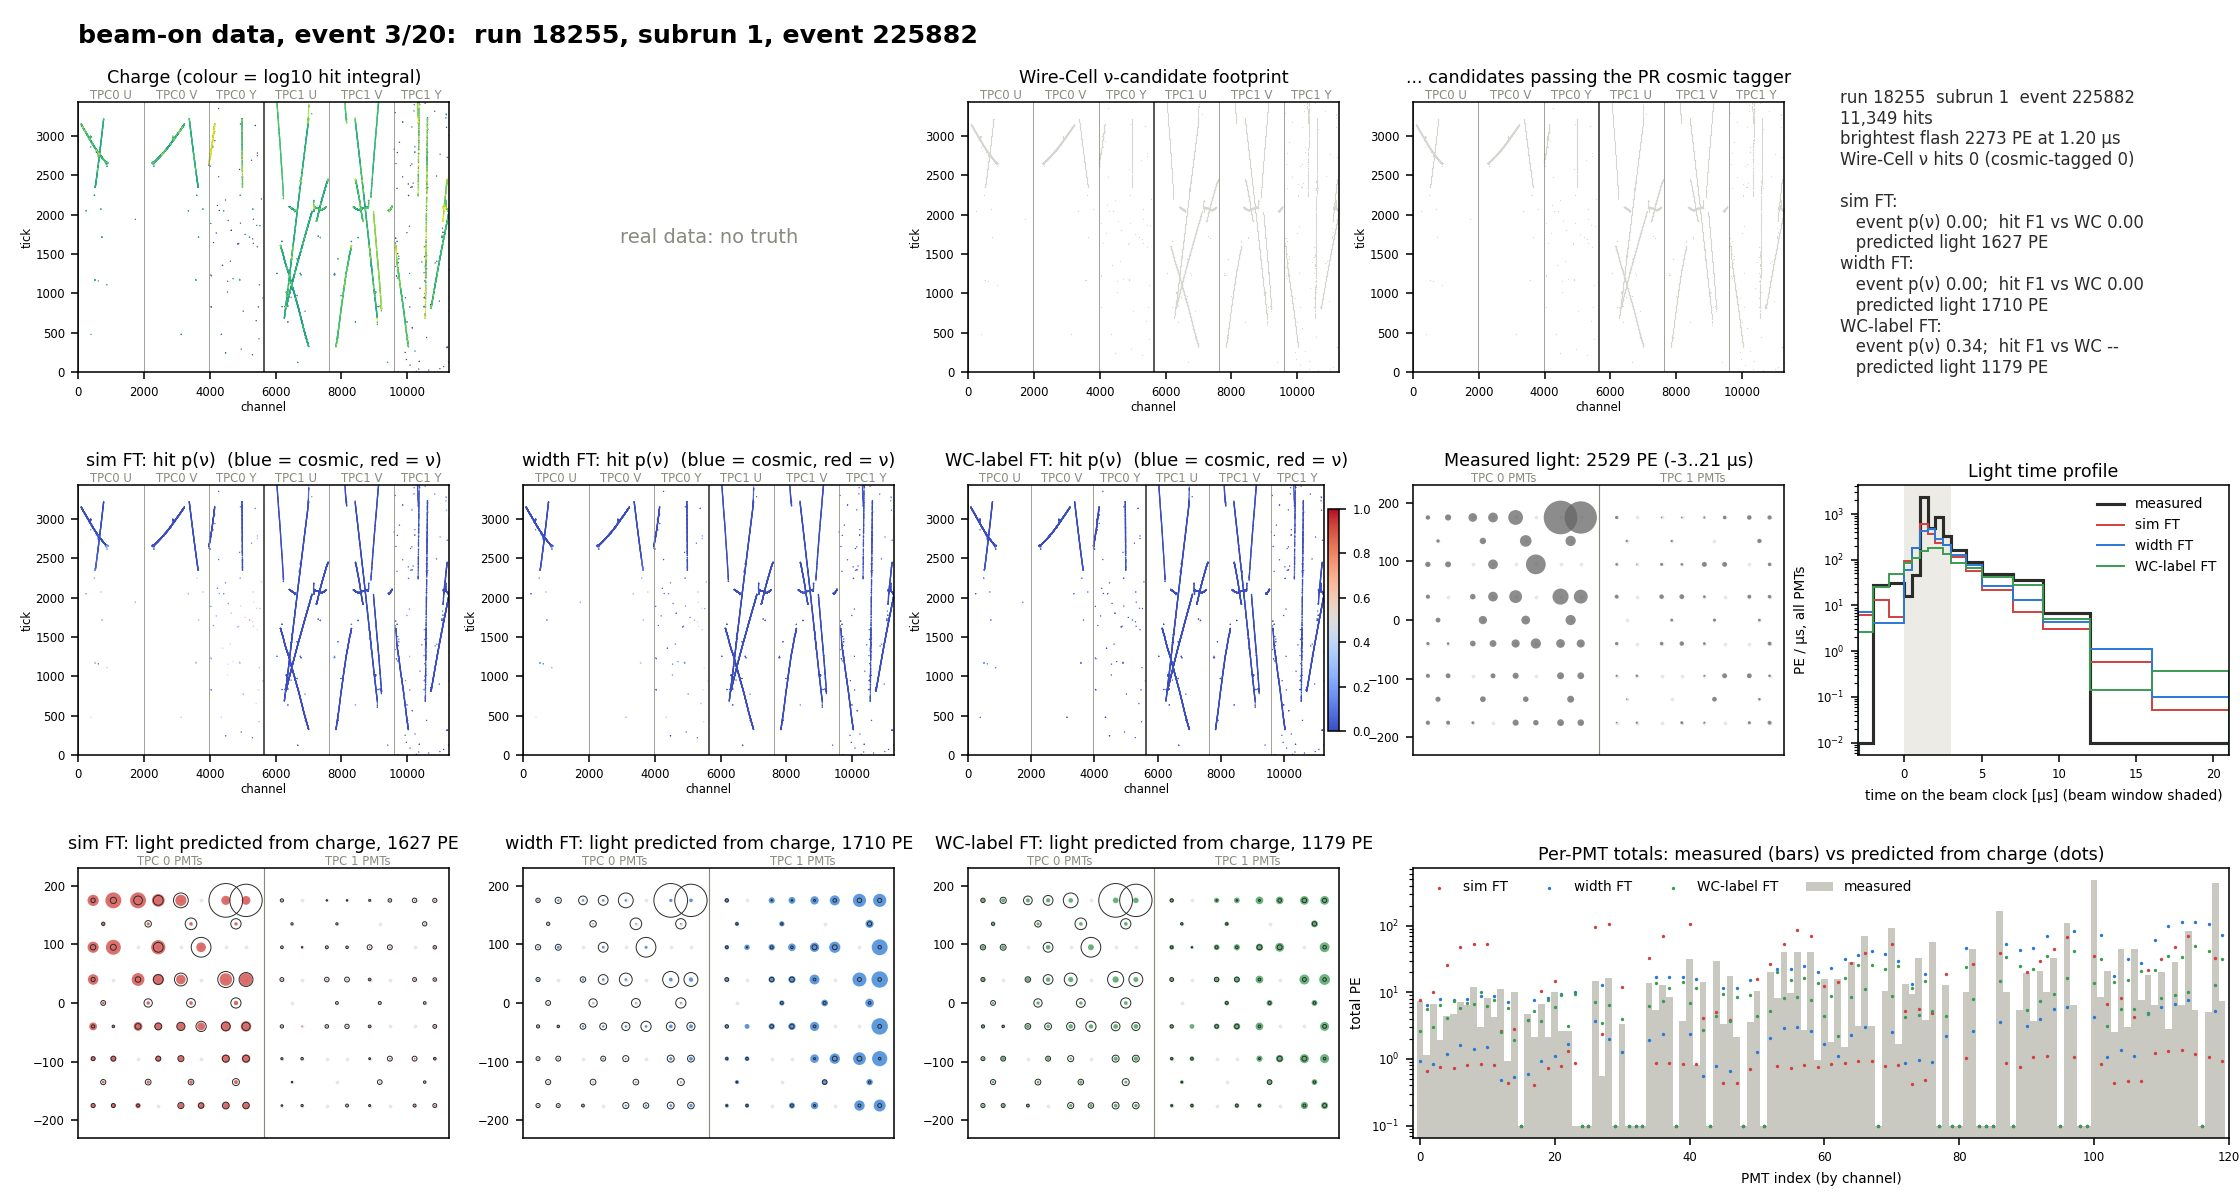
\includegraphics[width=\paperwidth,height=\paperheight,keepaspectratio]{displays/on_02.jpg}}
\end{frame}
% Beam-on data 4/20: run 18255, subrun 1, event 513616; event p(nu): sim FT 0.00, width FT 0.00, WC-label FT 0.04
\begin{frame}[plain]
  \centering\vspace*{-2pt}
  \makebox[\linewidth][c]{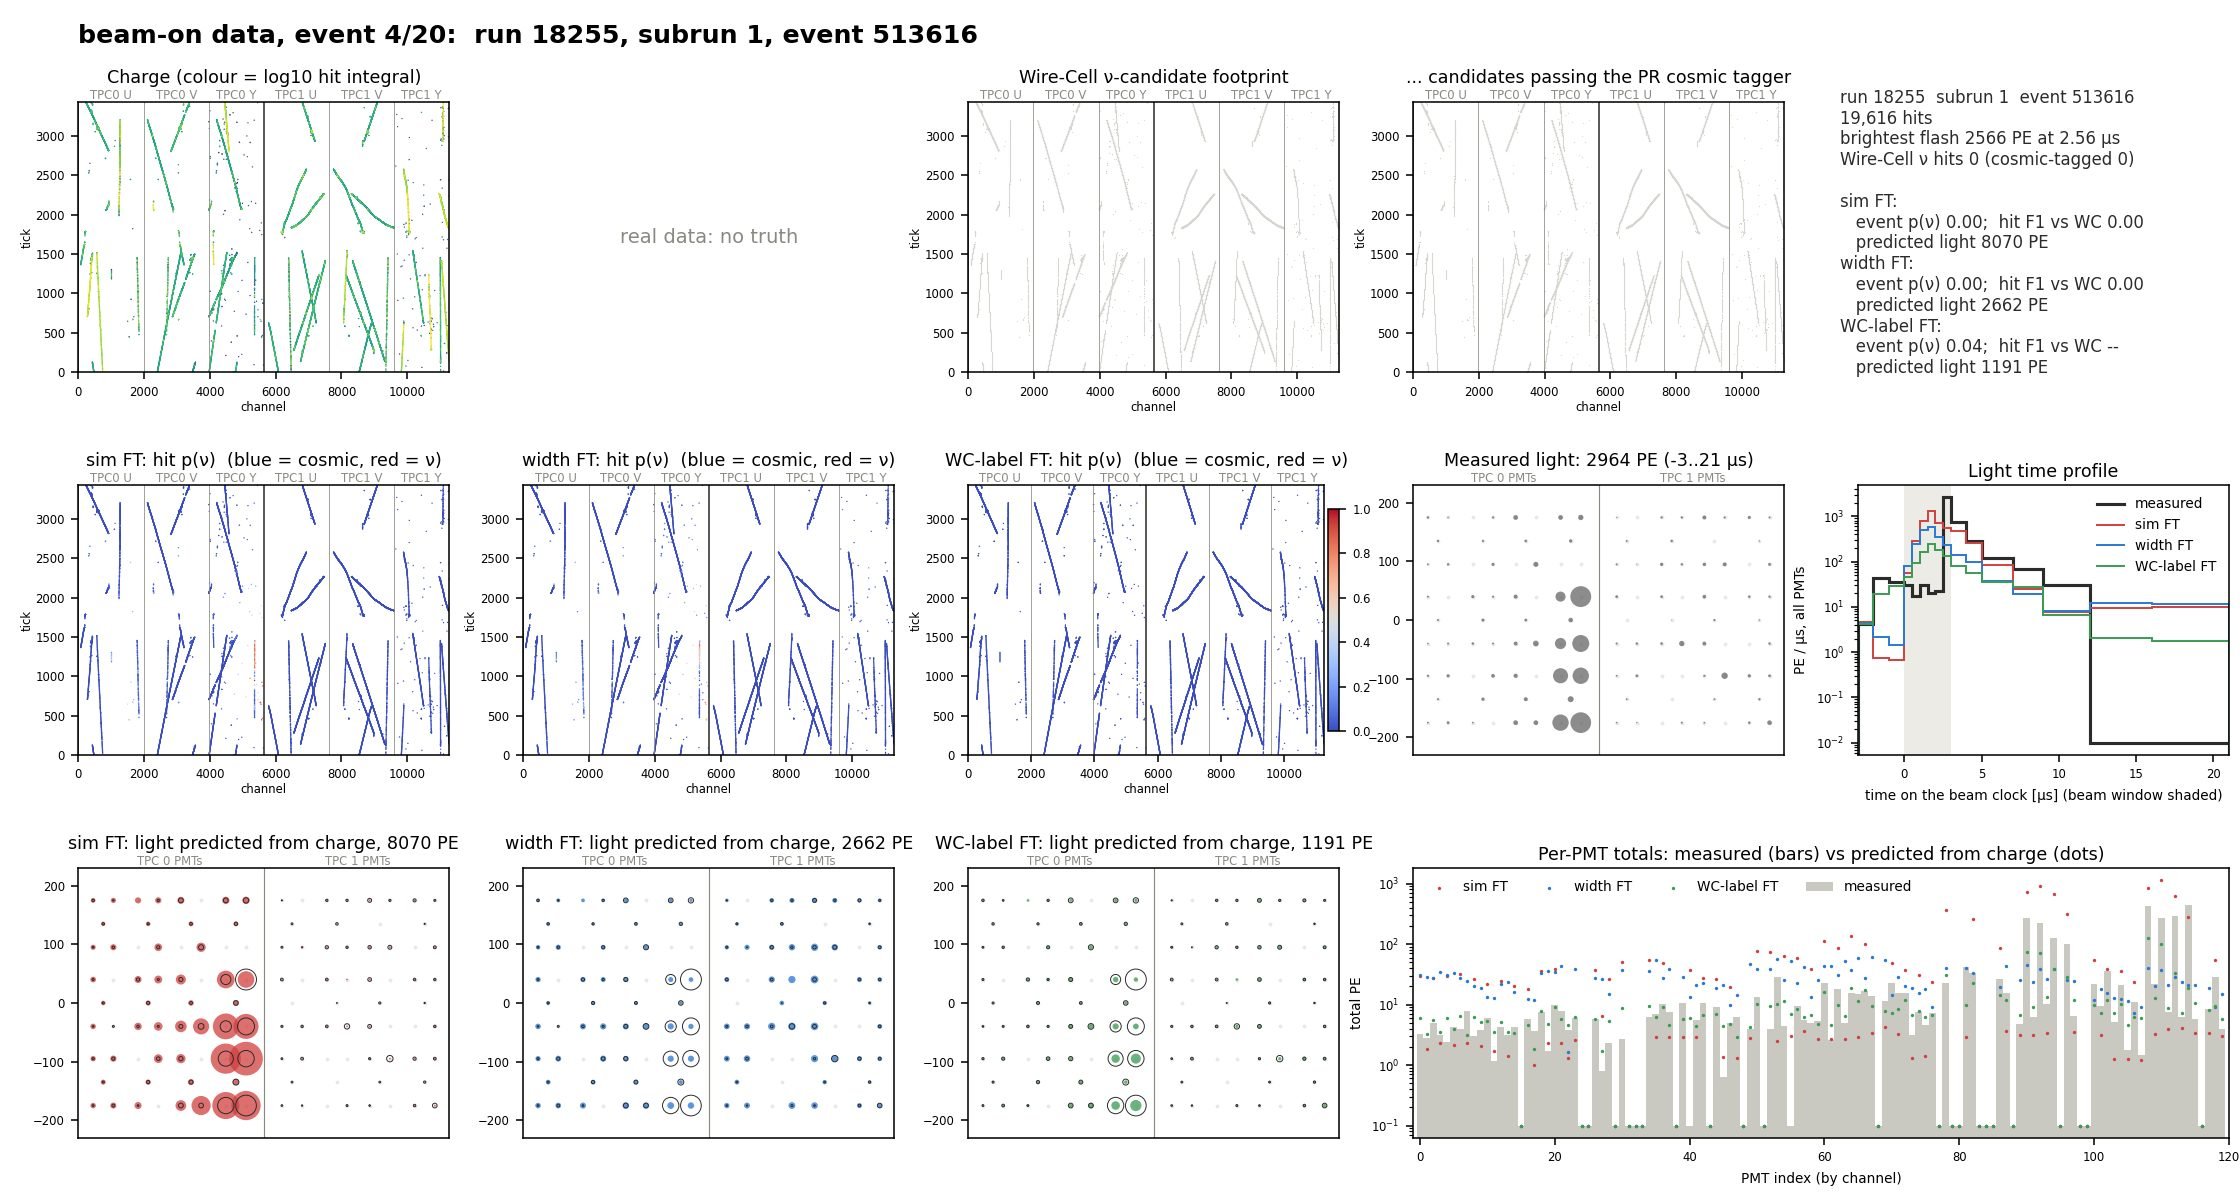
\includegraphics[width=\paperwidth,height=\paperheight,keepaspectratio]{displays/on_03.jpg}}
\end{frame}
% Beam-on data 5/20: run 18255, subrun 1, event 272264; event p(nu): sim FT 1.00, width FT 1.00, WC-label FT 0.96
\begin{frame}[plain]
  \centering\vspace*{-2pt}
  \makebox[\linewidth][c]{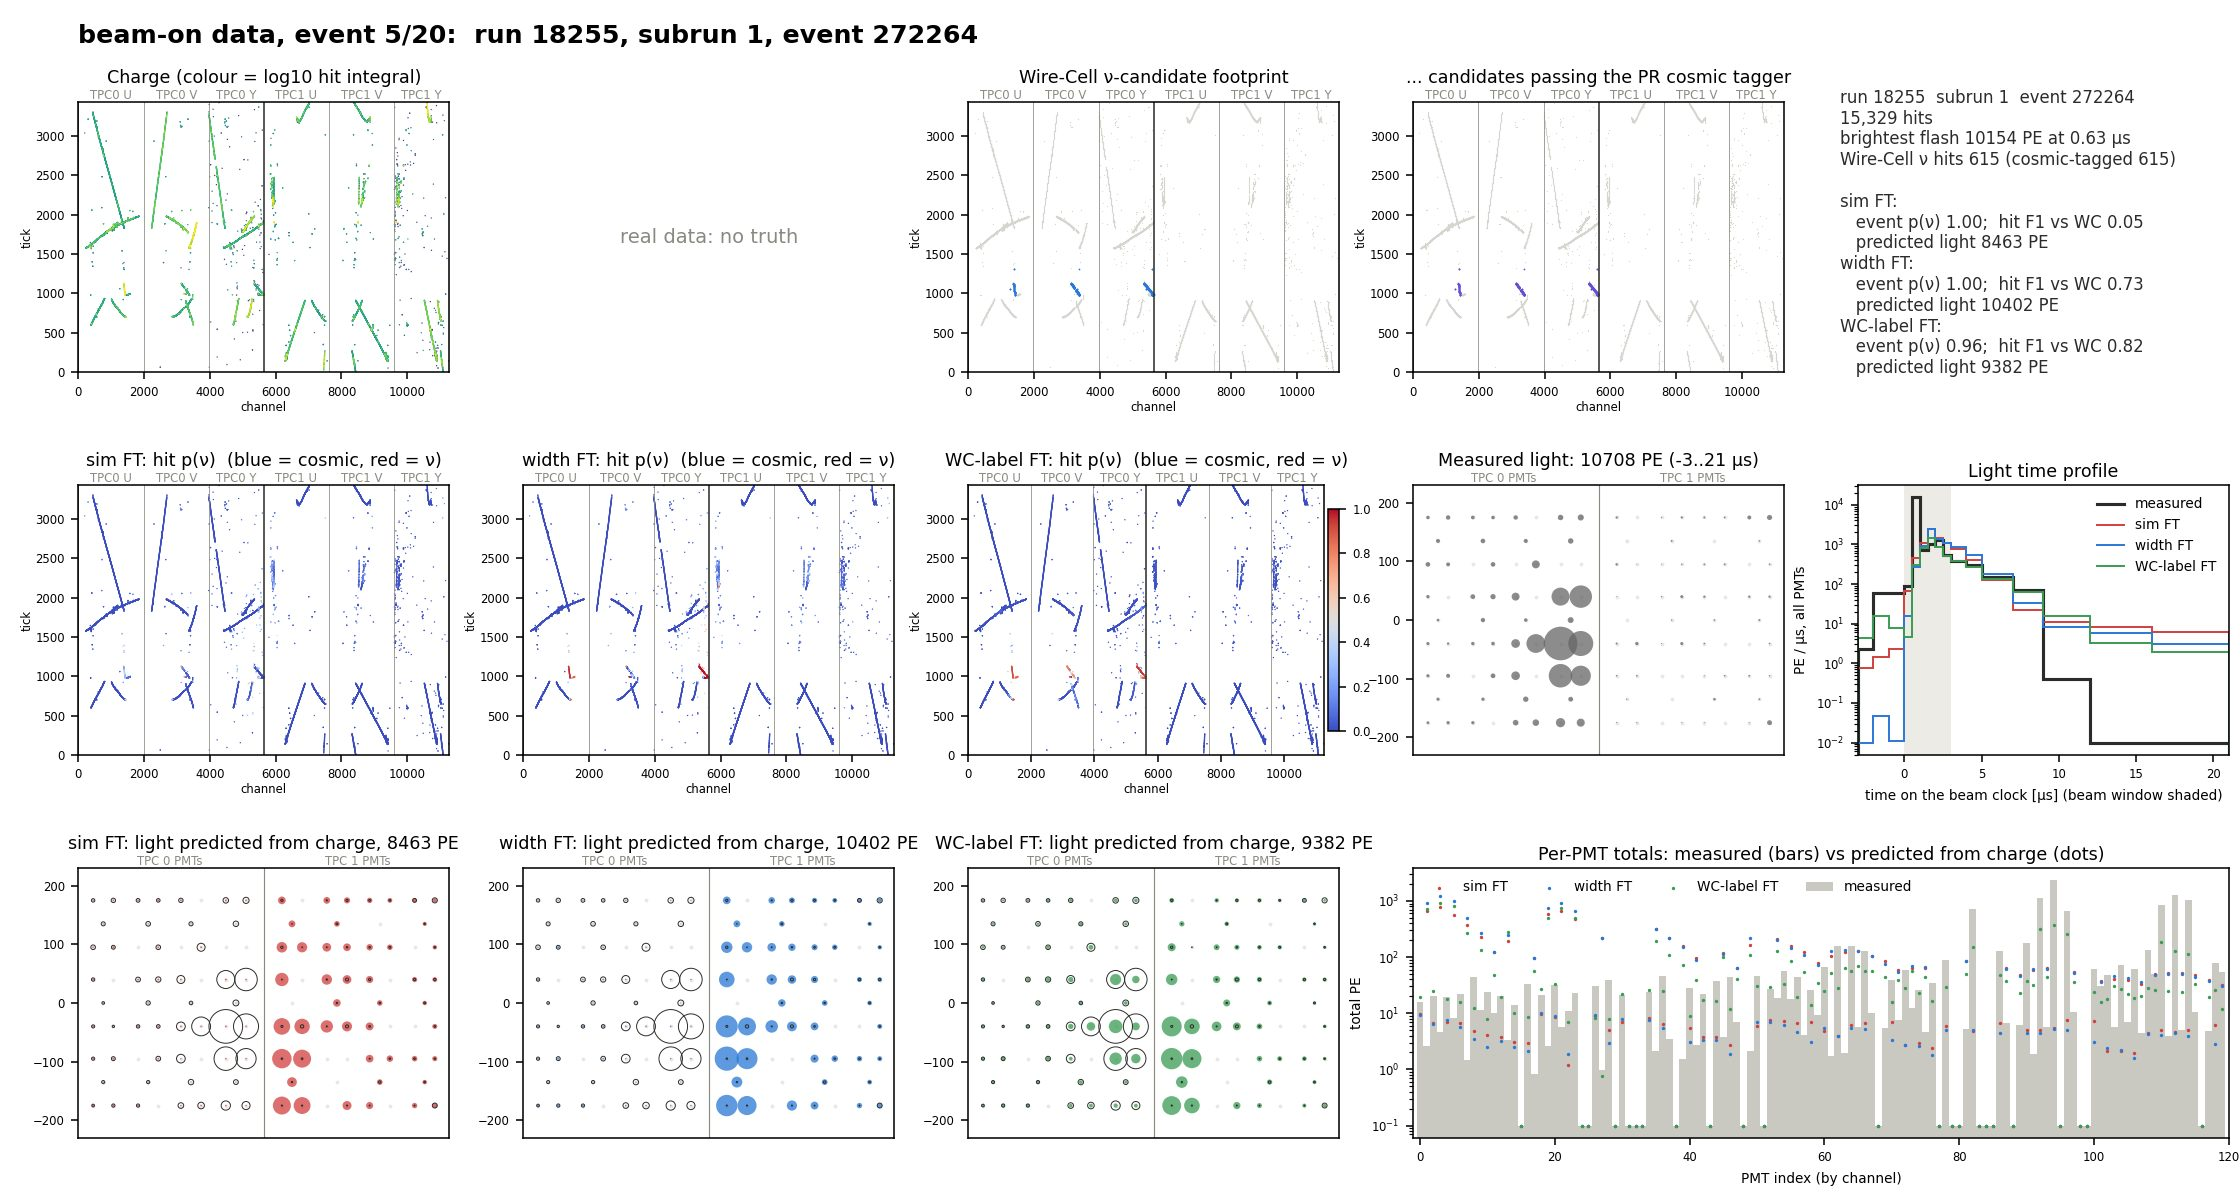
\includegraphics[width=\paperwidth,height=\paperheight,keepaspectratio]{displays/on_04.jpg}}
\end{frame}
% Beam-on data 6/20: run 18255, subrun 1, event 447683; event p(nu): sim FT 0.00, width FT 0.00, WC-label FT 0.84
\begin{frame}[plain]
  \centering\vspace*{-2pt}
  \makebox[\linewidth][c]{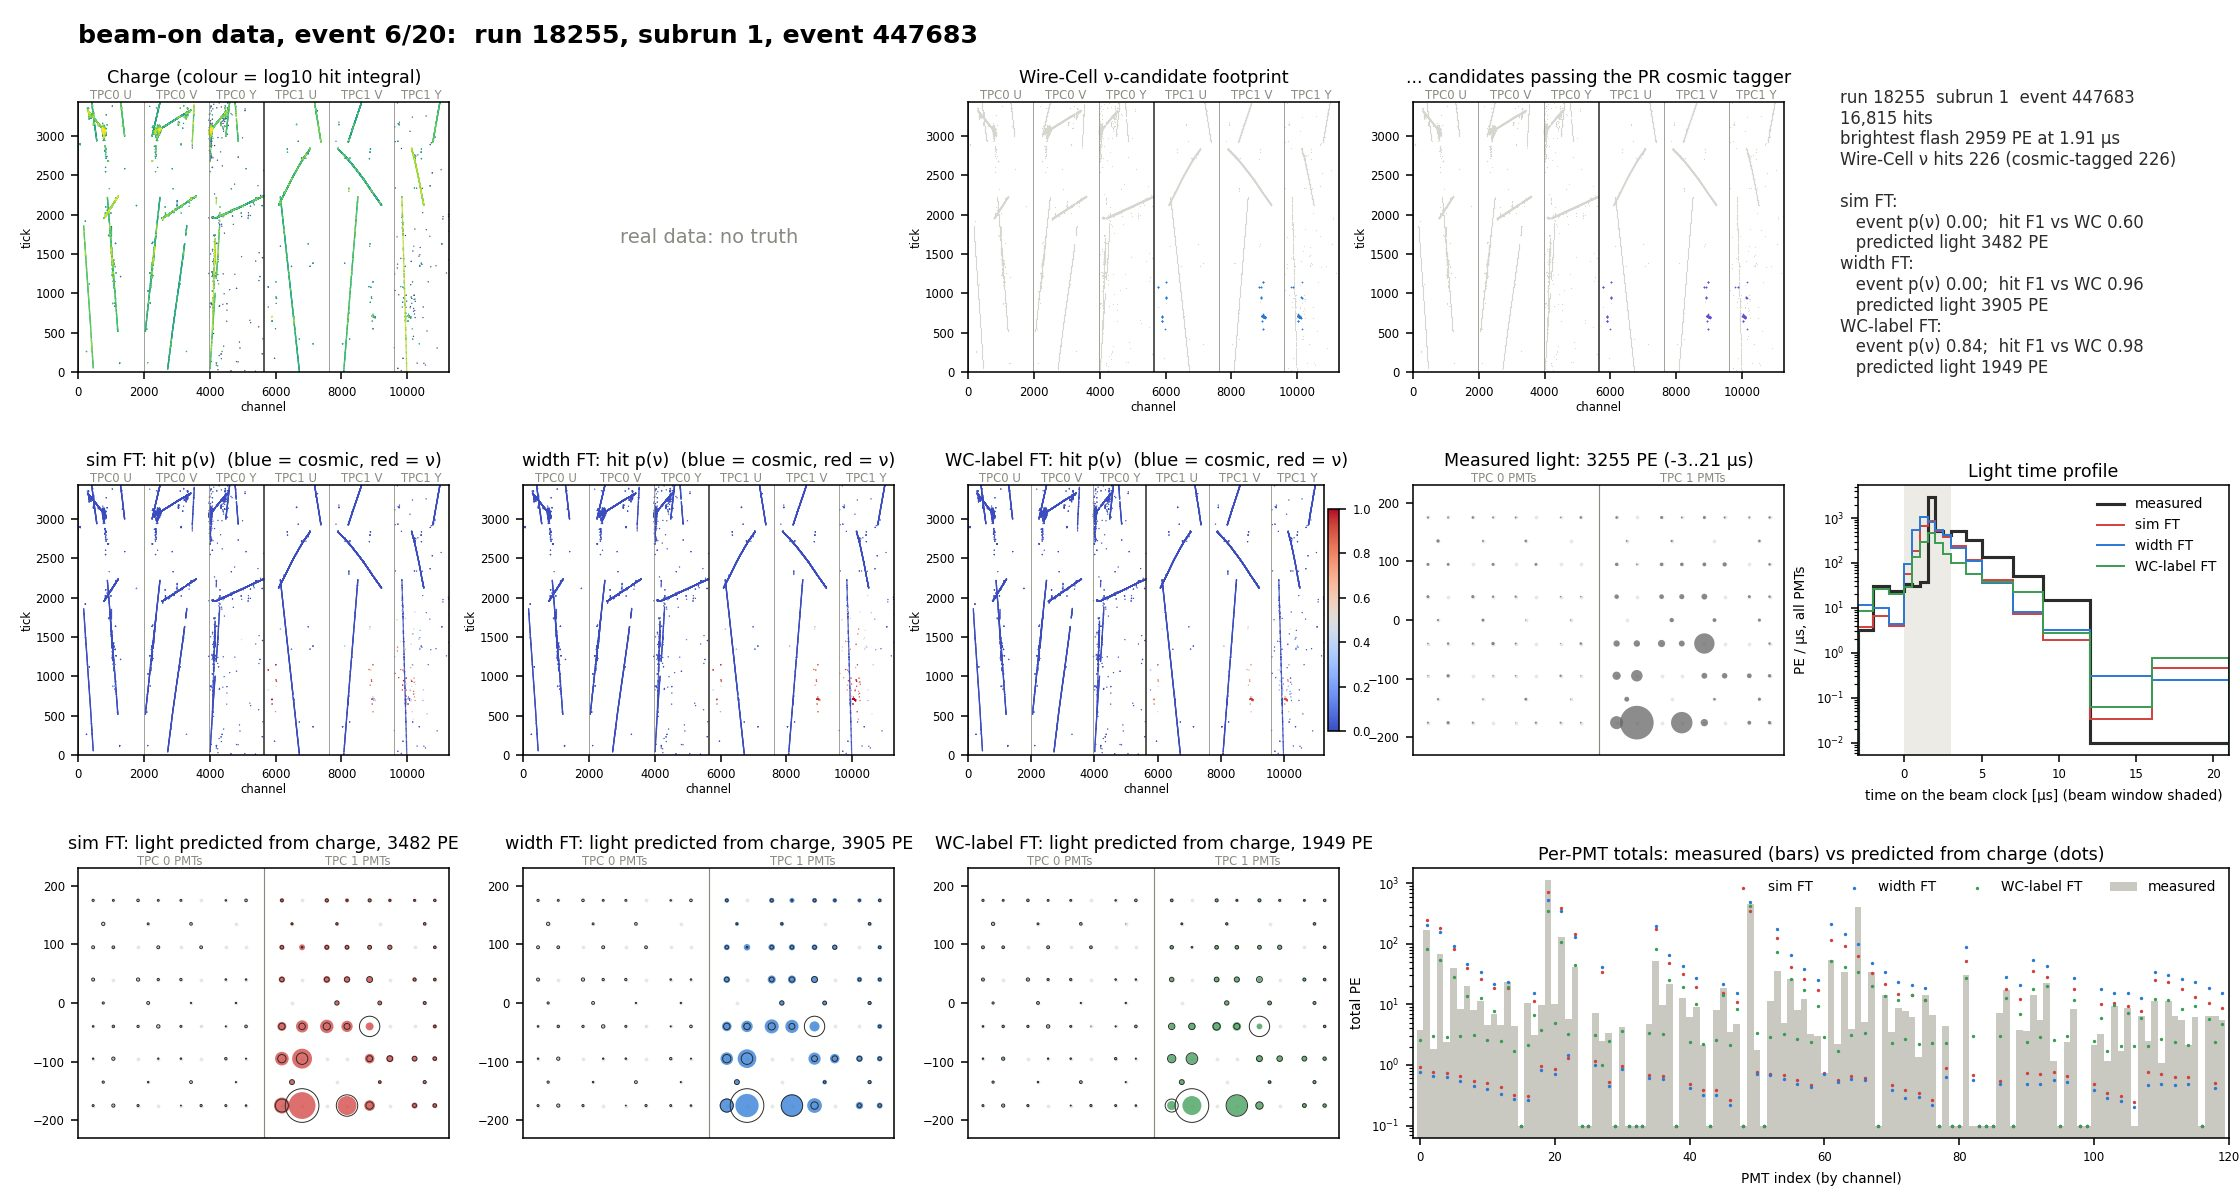
\includegraphics[width=\paperwidth,height=\paperheight,keepaspectratio]{displays/on_05.jpg}}
\end{frame}
% Beam-on data 7/20: run 18259, subrun 1, event 255438; event p(nu): sim FT 1.00, width FT 1.00, WC-label FT 0.97
\begin{frame}[plain]
  \centering\vspace*{-2pt}
  \makebox[\linewidth][c]{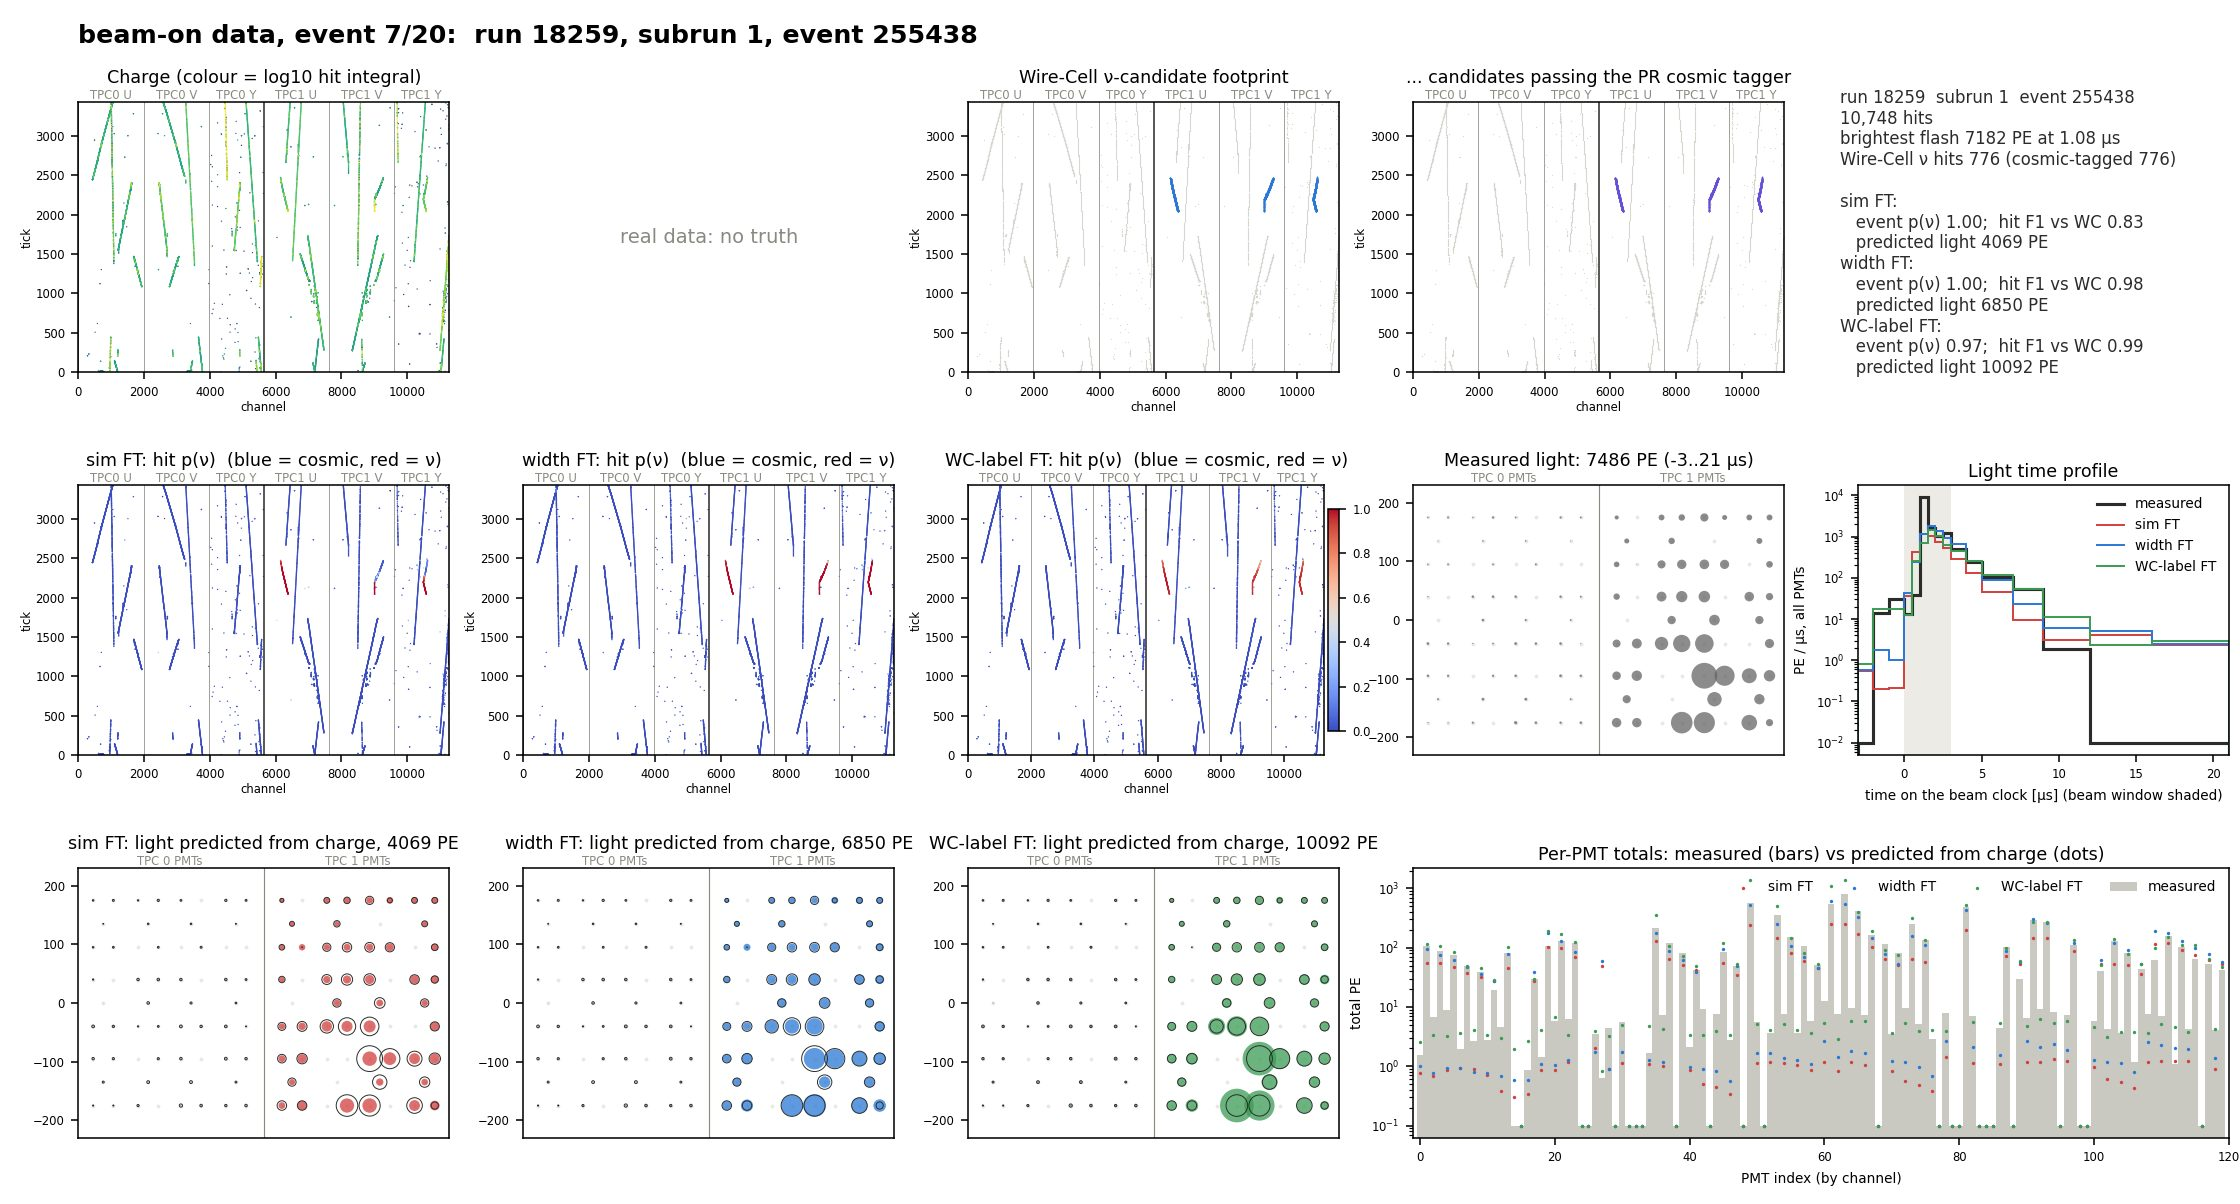
\includegraphics[width=\paperwidth,height=\paperheight,keepaspectratio]{displays/on_06.jpg}}
\end{frame}
% Beam-on data 8/20: run 18255, subrun 1, event 486168; event p(nu): sim FT 0.99, width FT 1.00, WC-label FT 0.93
\begin{frame}[plain]
  \centering\vspace*{-2pt}
  \makebox[\linewidth][c]{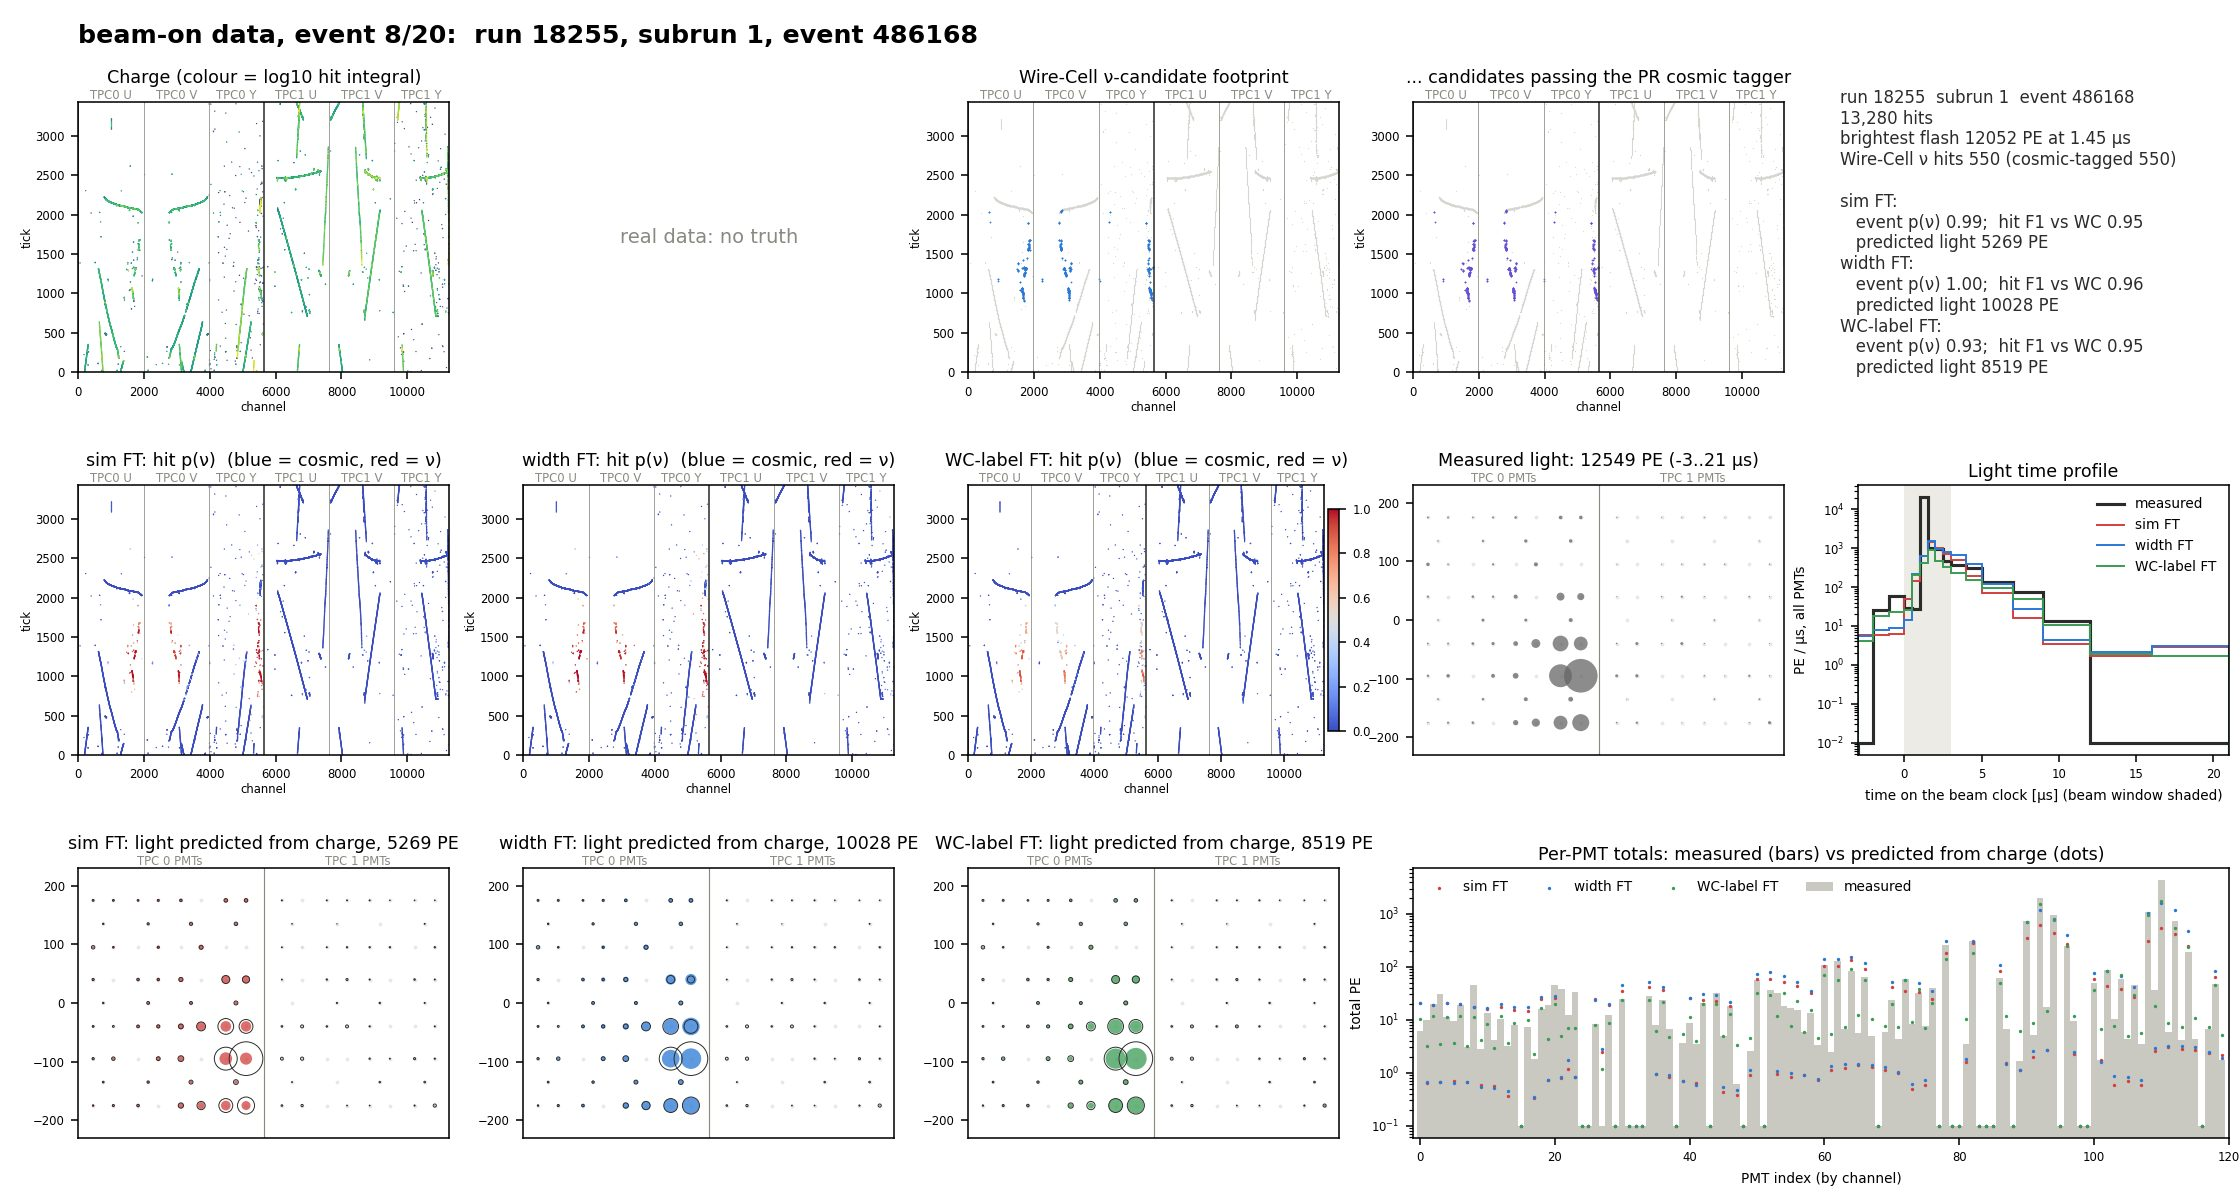
\includegraphics[width=\paperwidth,height=\paperheight,keepaspectratio]{displays/on_07.jpg}}
\end{frame}
% Beam-on data 9/20: run 18255, subrun 1, event 28768; event p(nu): sim FT 0.00, width FT 0.00, WC-label FT 0.08
\begin{frame}[plain]
  \centering\vspace*{-2pt}
  \makebox[\linewidth][c]{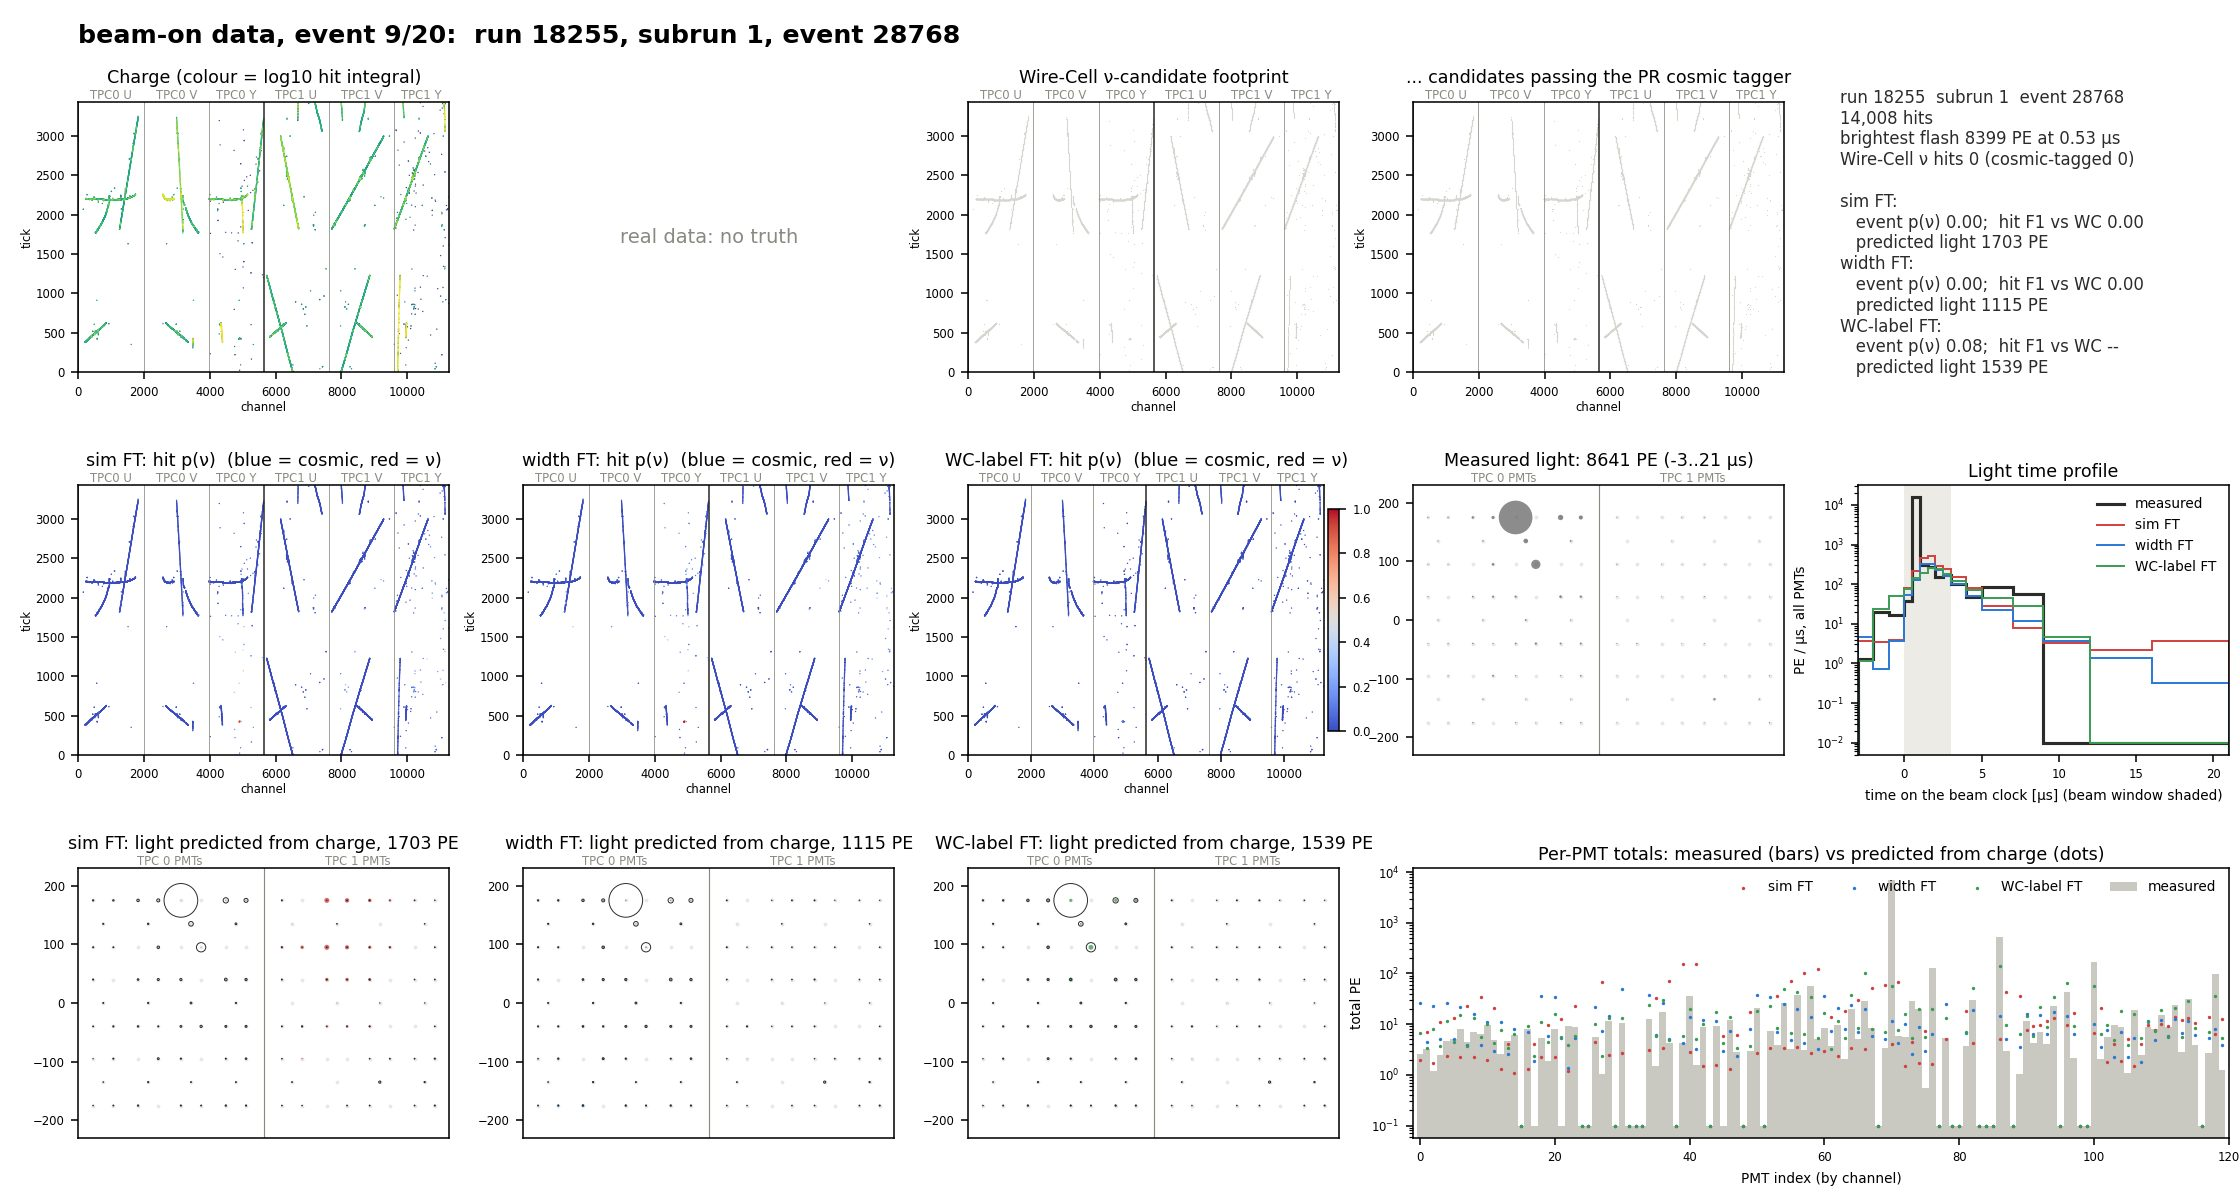
\includegraphics[width=\paperwidth,height=\paperheight,keepaspectratio]{displays/on_08.jpg}}
\end{frame}
% Beam-on data 10/20: run 18259, subrun 1, event 258582; event p(nu): sim FT 0.00, width FT 0.00, WC-label FT 0.34
\begin{frame}[plain]
  \centering\vspace*{-2pt}
  \makebox[\linewidth][c]{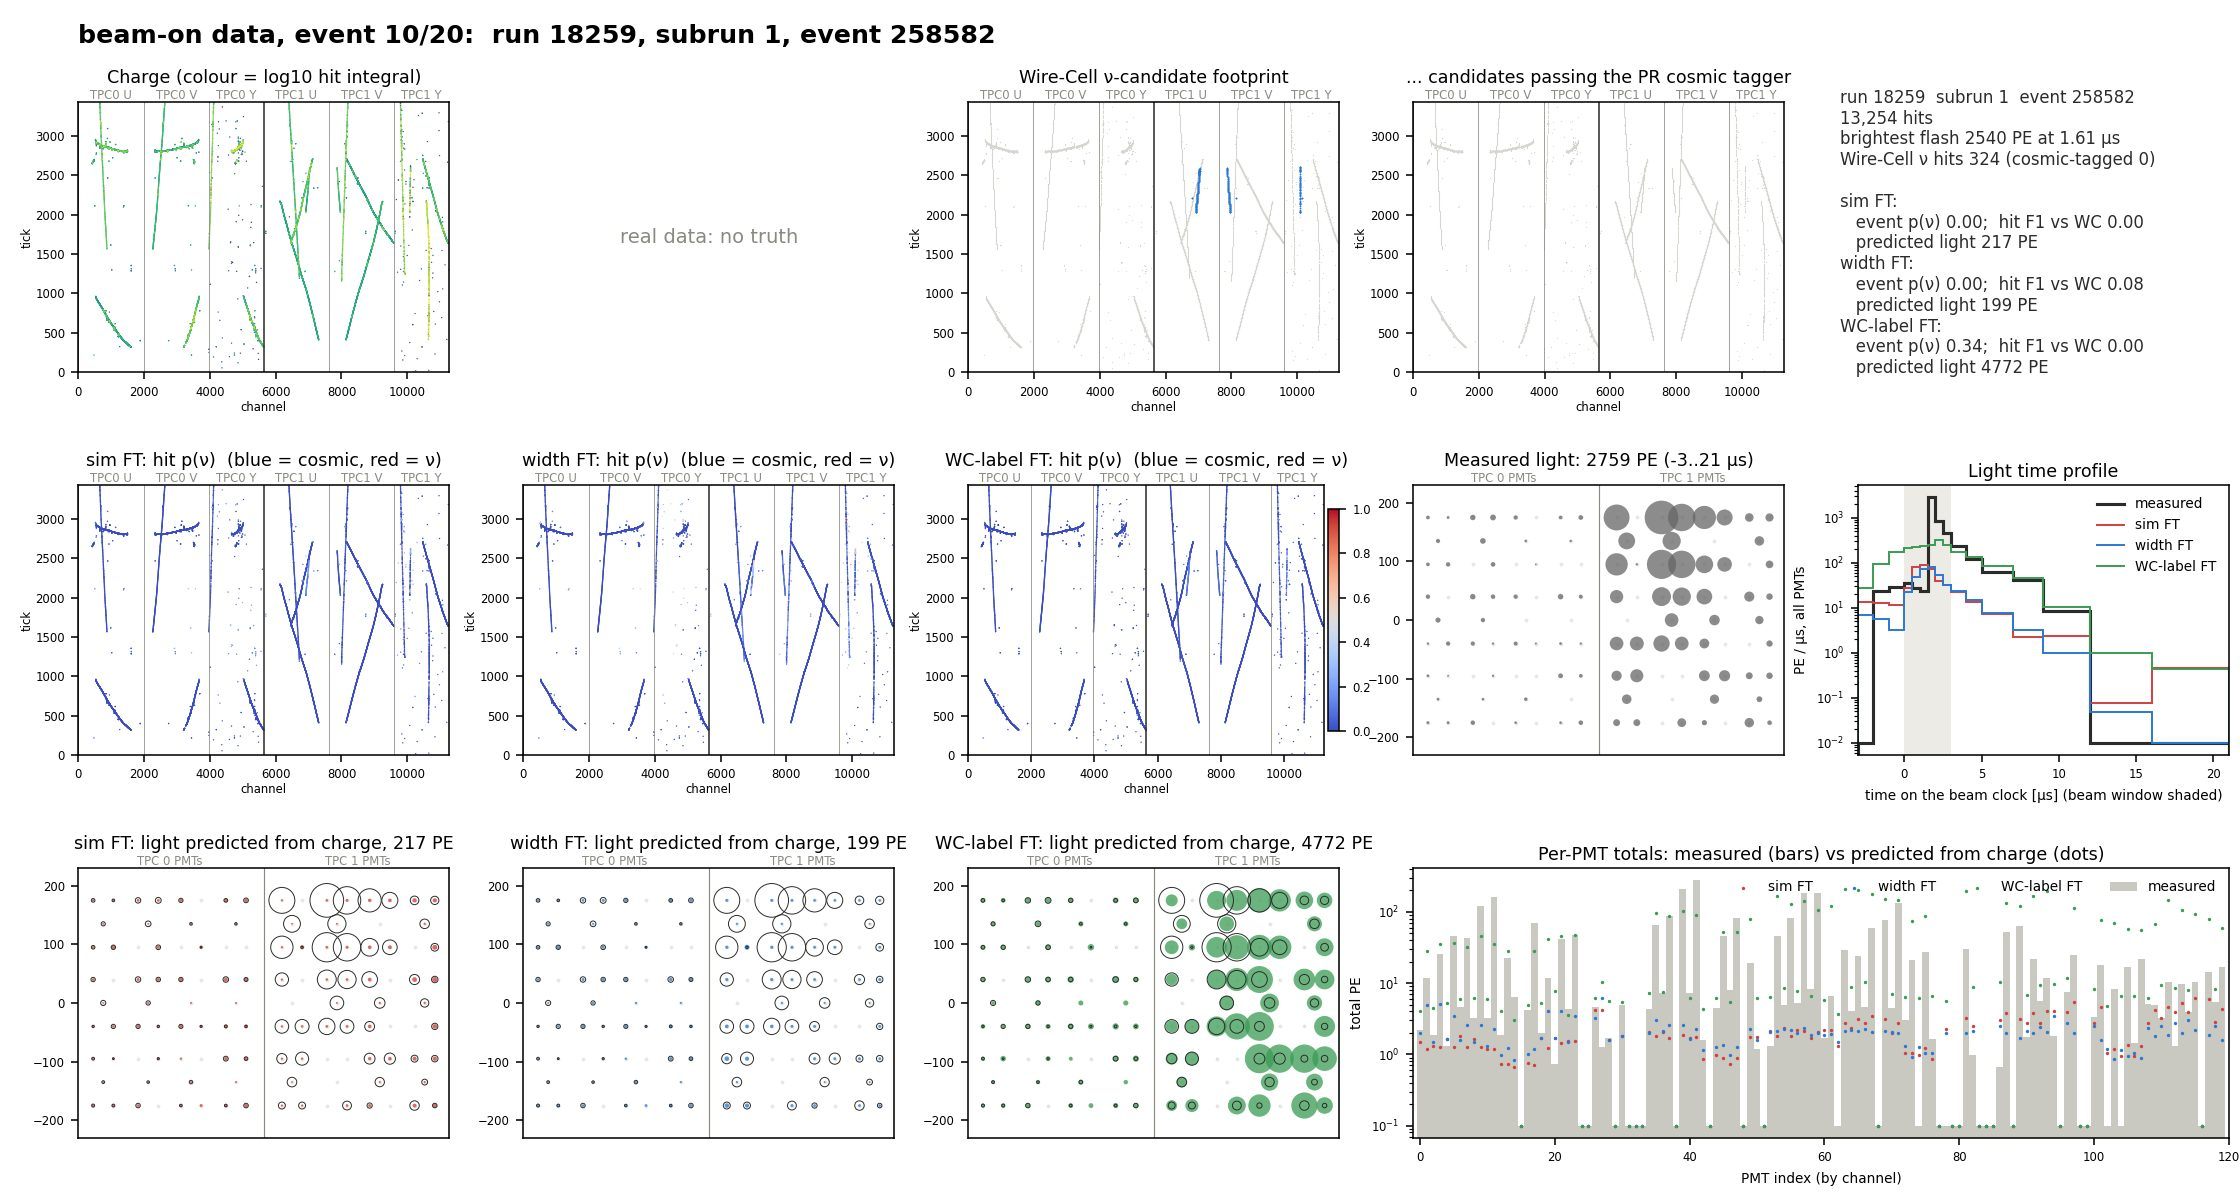
\includegraphics[width=\paperwidth,height=\paperheight,keepaspectratio]{displays/on_09.jpg}}
\end{frame}
% Beam-on data 11/20: run 18255, subrun 1, event 122922; event p(nu): sim FT 0.99, width FT 1.00, WC-label FT 0.17
\begin{frame}[plain]
  \centering\vspace*{-2pt}
  \makebox[\linewidth][c]{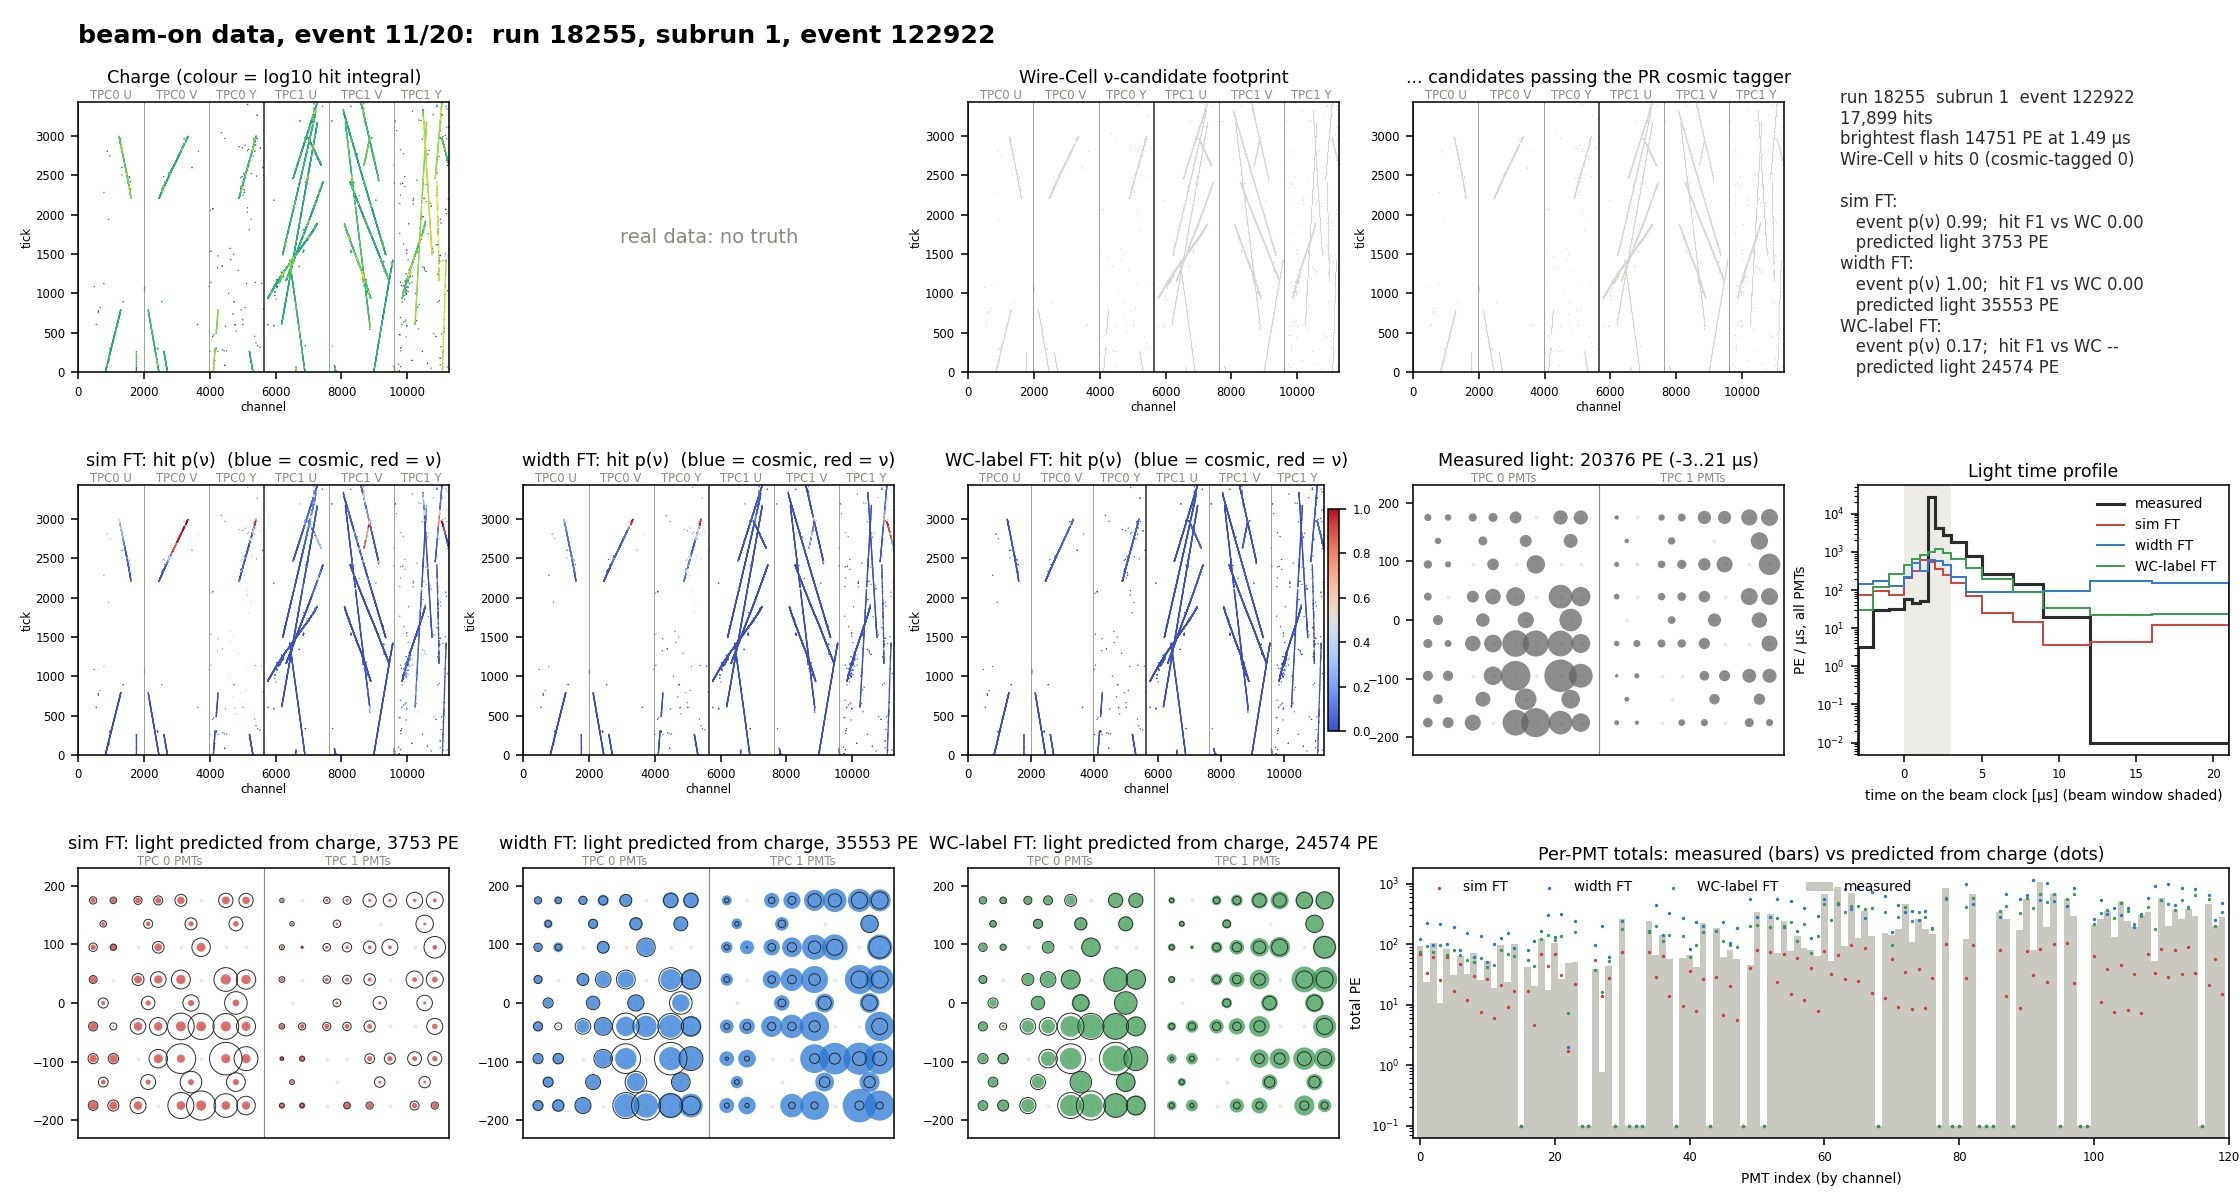
\includegraphics[width=\paperwidth,height=\paperheight,keepaspectratio]{displays/on_10.jpg}}
\end{frame}
% Beam-on data 12/20: run 18255, subrun 1, event 393542; event p(nu): sim FT 0.00, width FT 0.00, WC-label FT 0.49
\begin{frame}[plain]
  \centering\vspace*{-2pt}
  \makebox[\linewidth][c]{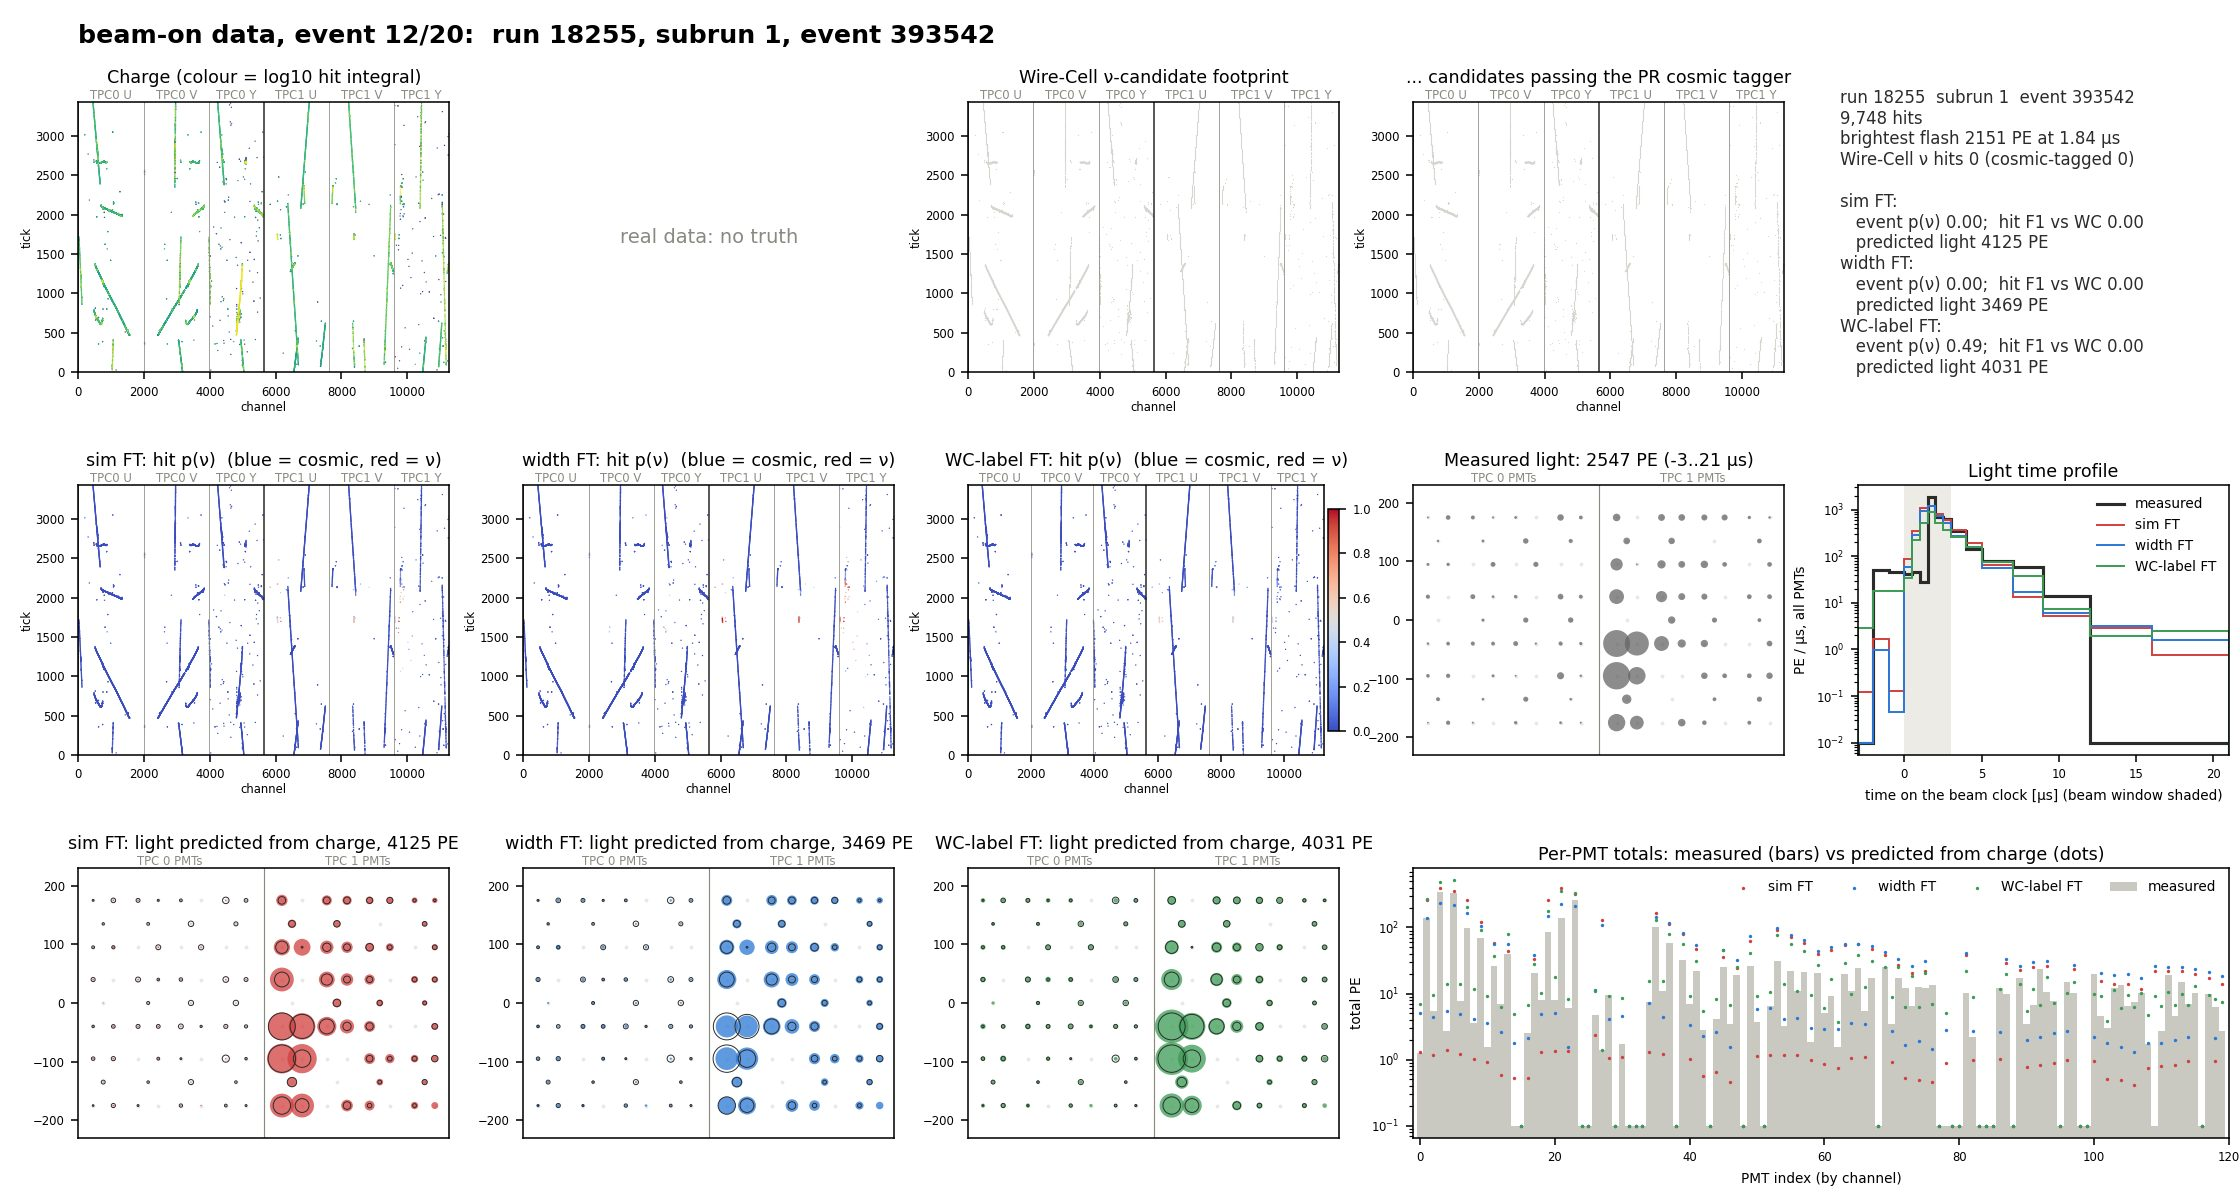
\includegraphics[width=\paperwidth,height=\paperheight,keepaspectratio]{displays/on_11.jpg}}
\end{frame}
% Beam-on data 13/20: run 18255, subrun 1, event 390700; event p(nu): sim FT 0.00, width FT 0.00, WC-label FT 0.11
\begin{frame}[plain]
  \centering\vspace*{-2pt}
  \makebox[\linewidth][c]{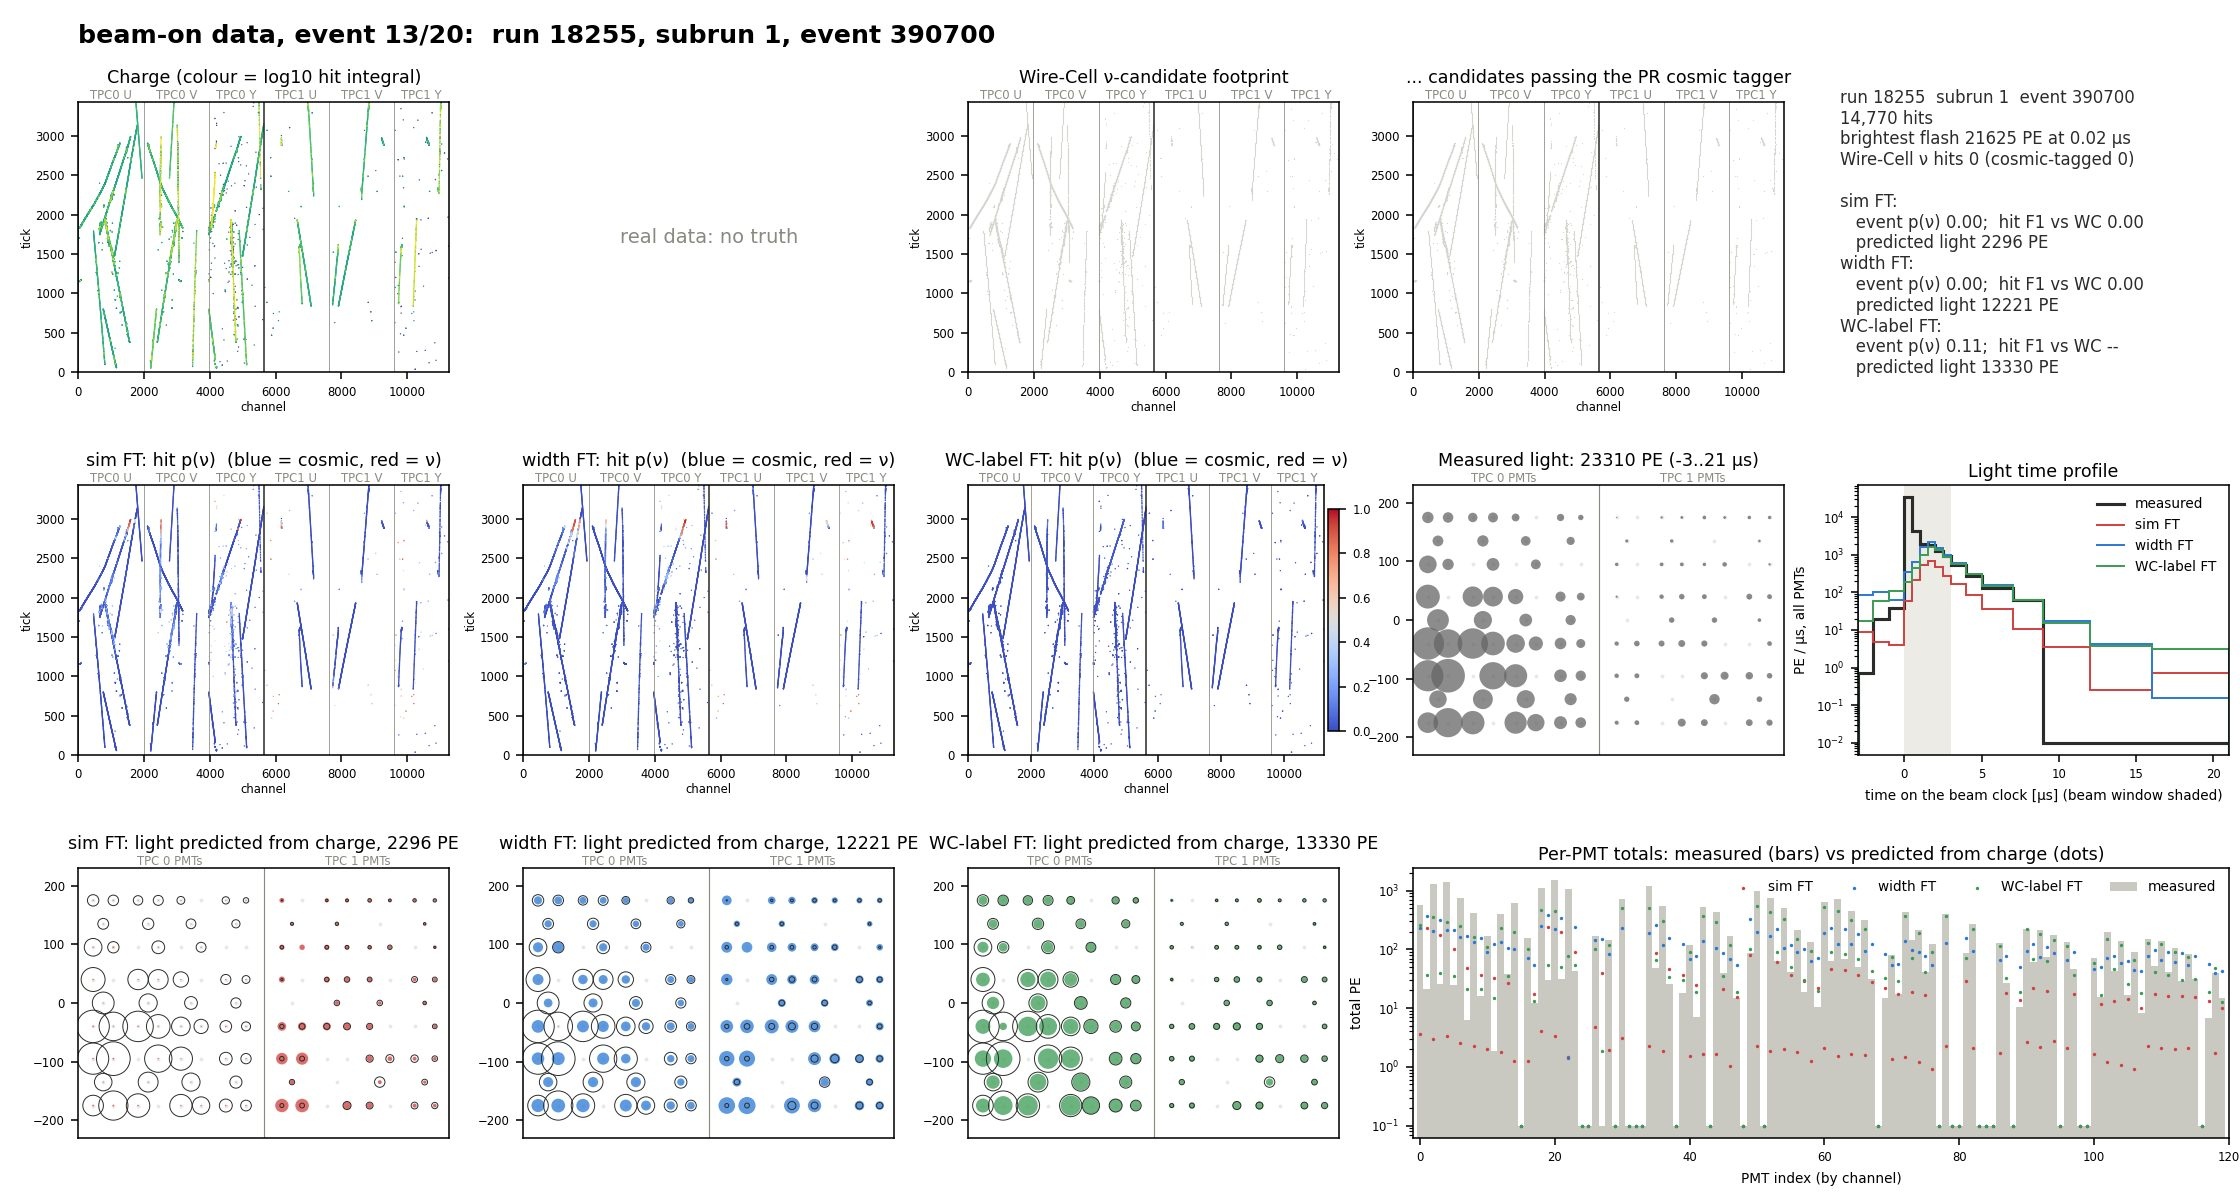
\includegraphics[width=\paperwidth,height=\paperheight,keepaspectratio]{displays/on_12.jpg}}
\end{frame}
% Beam-on data 14/20: run 18255, subrun 1, event 136435; event p(nu): sim FT 1.00, width FT 1.00, WC-label FT 0.99
\begin{frame}[plain]
  \centering\vspace*{-2pt}
  \makebox[\linewidth][c]{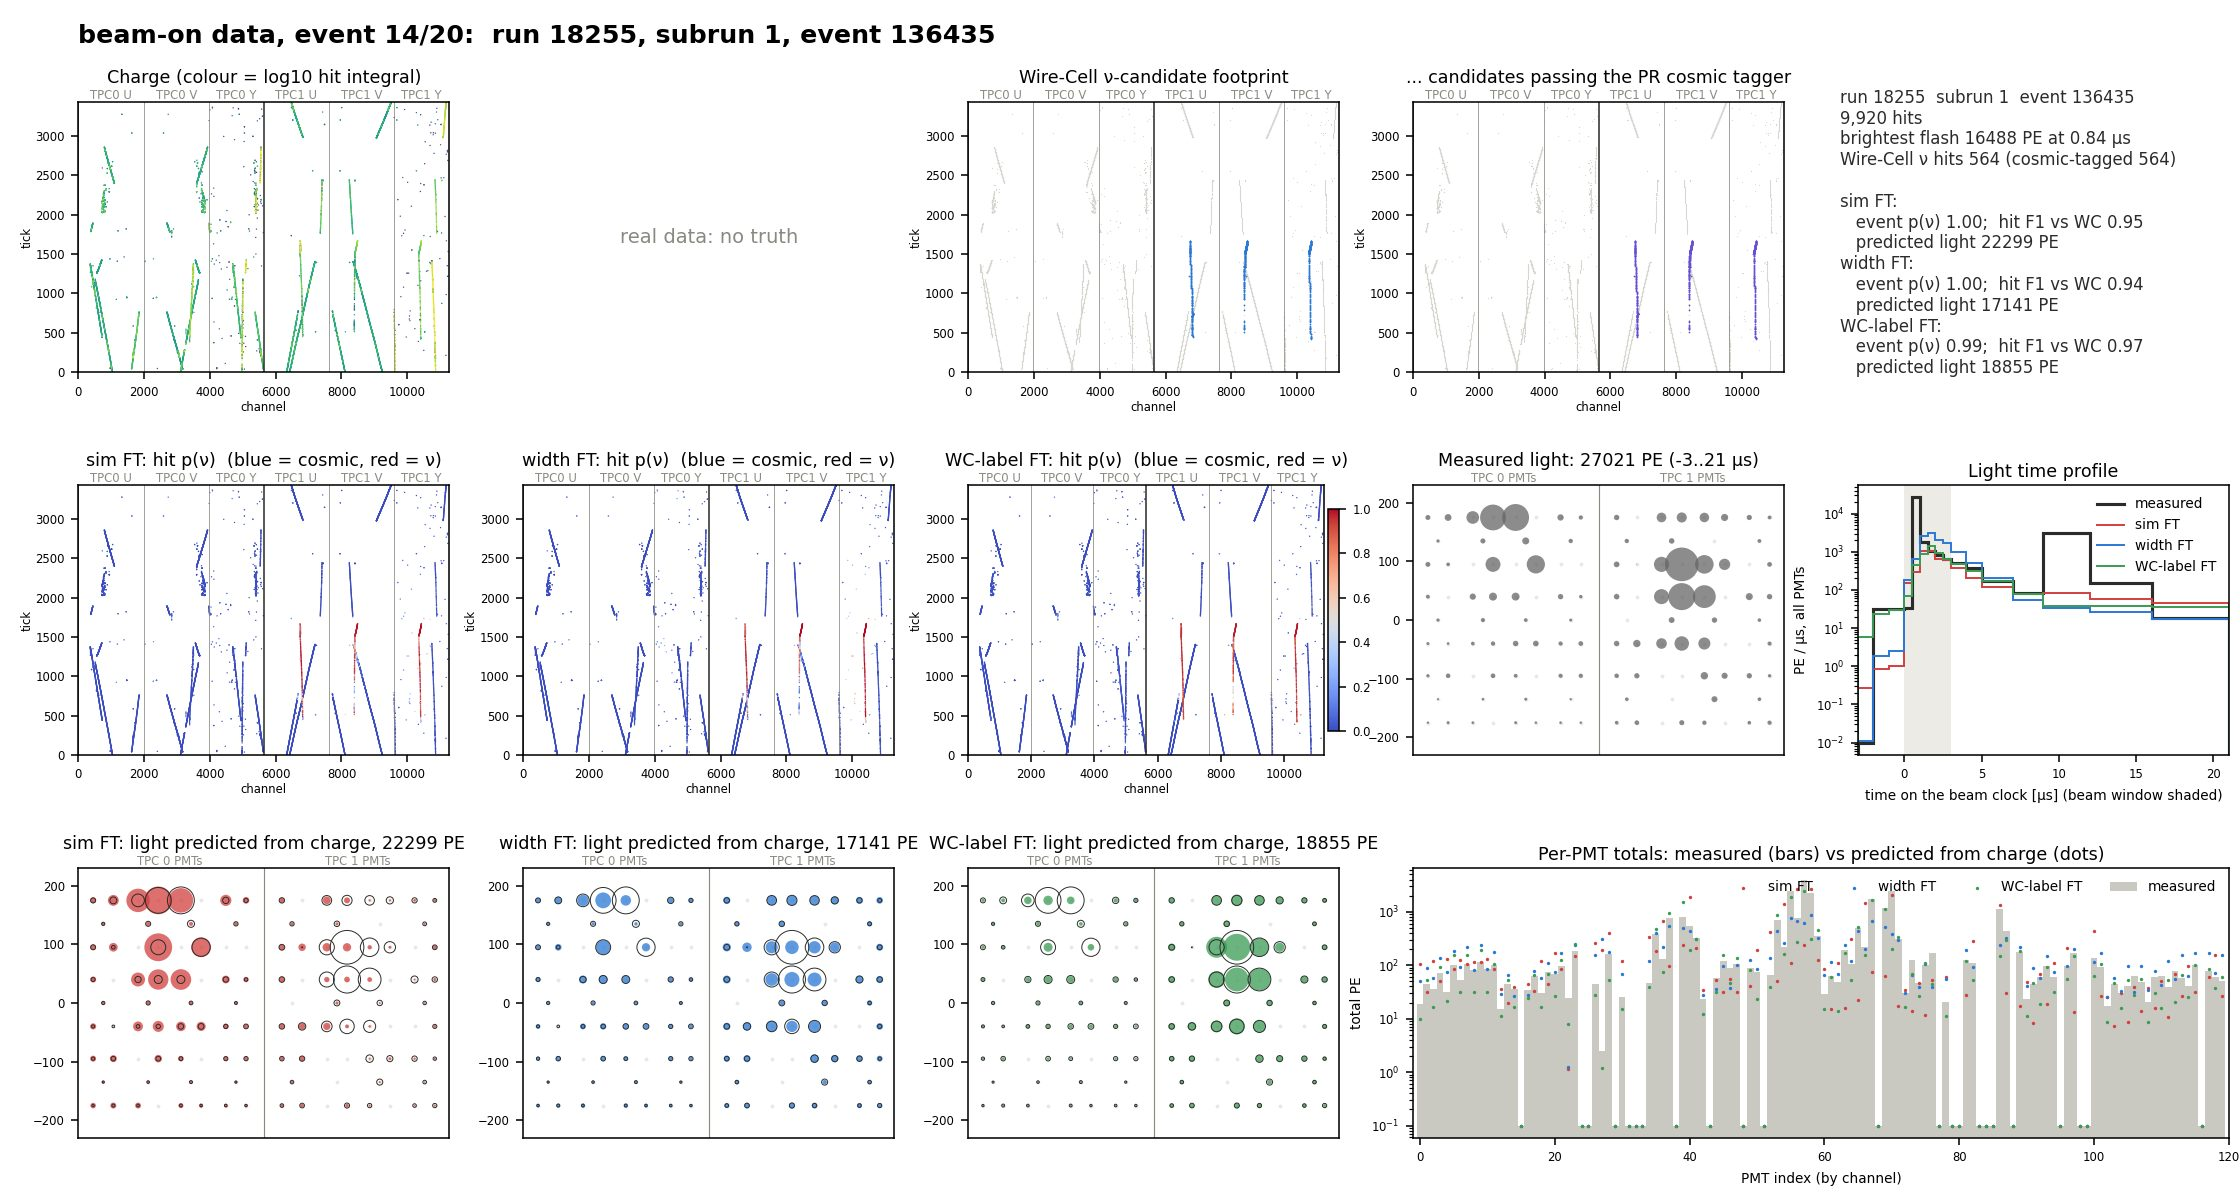
\includegraphics[width=\paperwidth,height=\paperheight,keepaspectratio]{displays/on_13.jpg}}
\end{frame}
% Beam-on data 15/20: run 18255, subrun 1, event 339420; event p(nu): sim FT 0.13, width FT 0.00, WC-label FT 0.80
\begin{frame}[plain]
  \centering\vspace*{-2pt}
  \makebox[\linewidth][c]{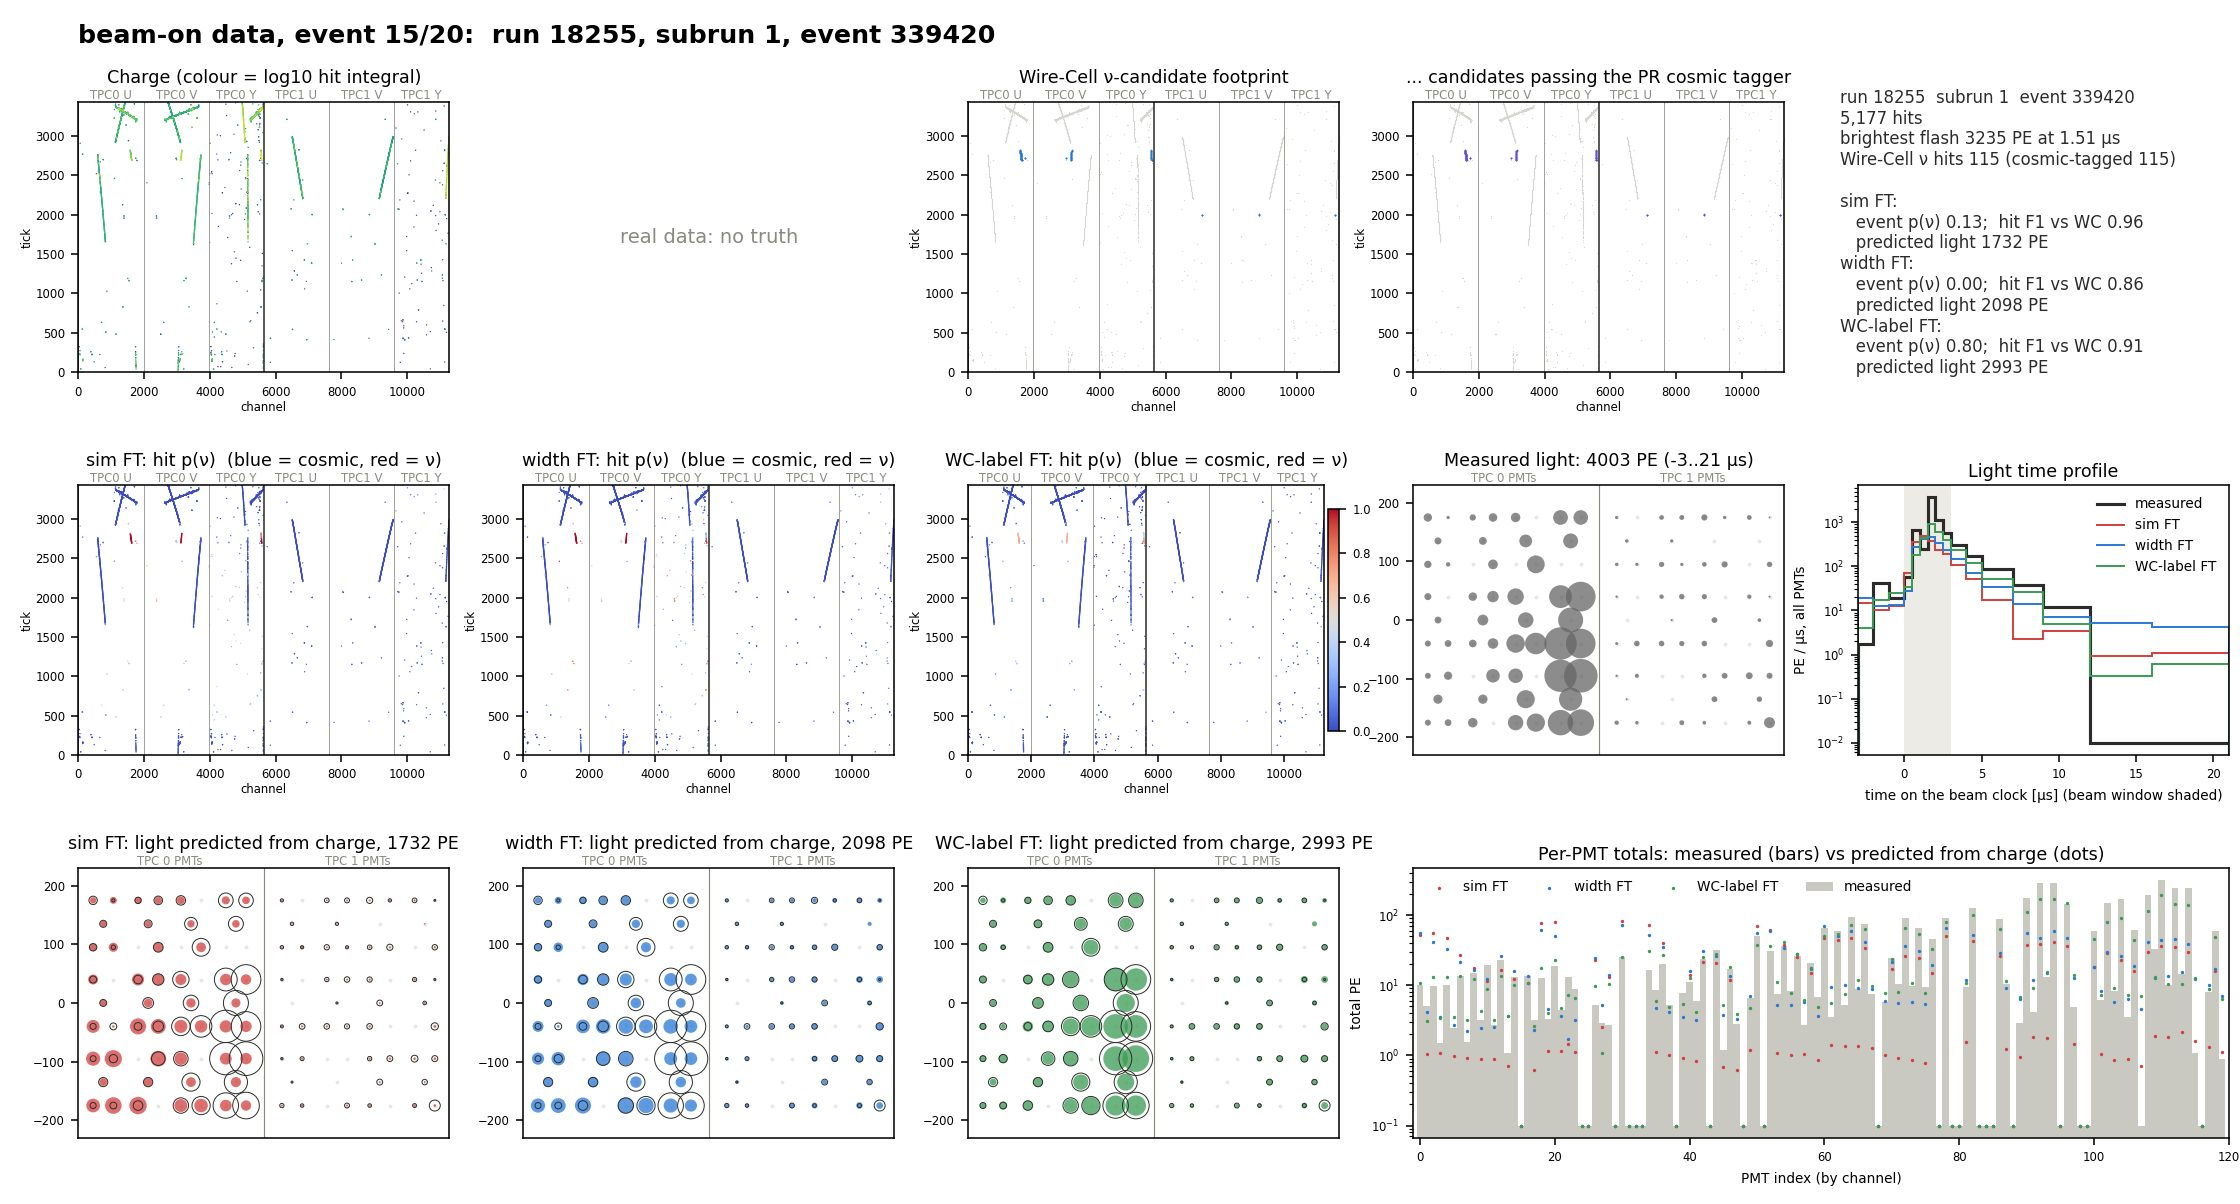
\includegraphics[width=\paperwidth,height=\paperheight,keepaspectratio]{displays/on_14.jpg}}
\end{frame}
% Beam-on data 16/20: run 18259, subrun 1, event 236590; event p(nu): sim FT 1.00, width FT 0.61, WC-label FT 0.72
\begin{frame}[plain]
  \centering\vspace*{-2pt}
  \makebox[\linewidth][c]{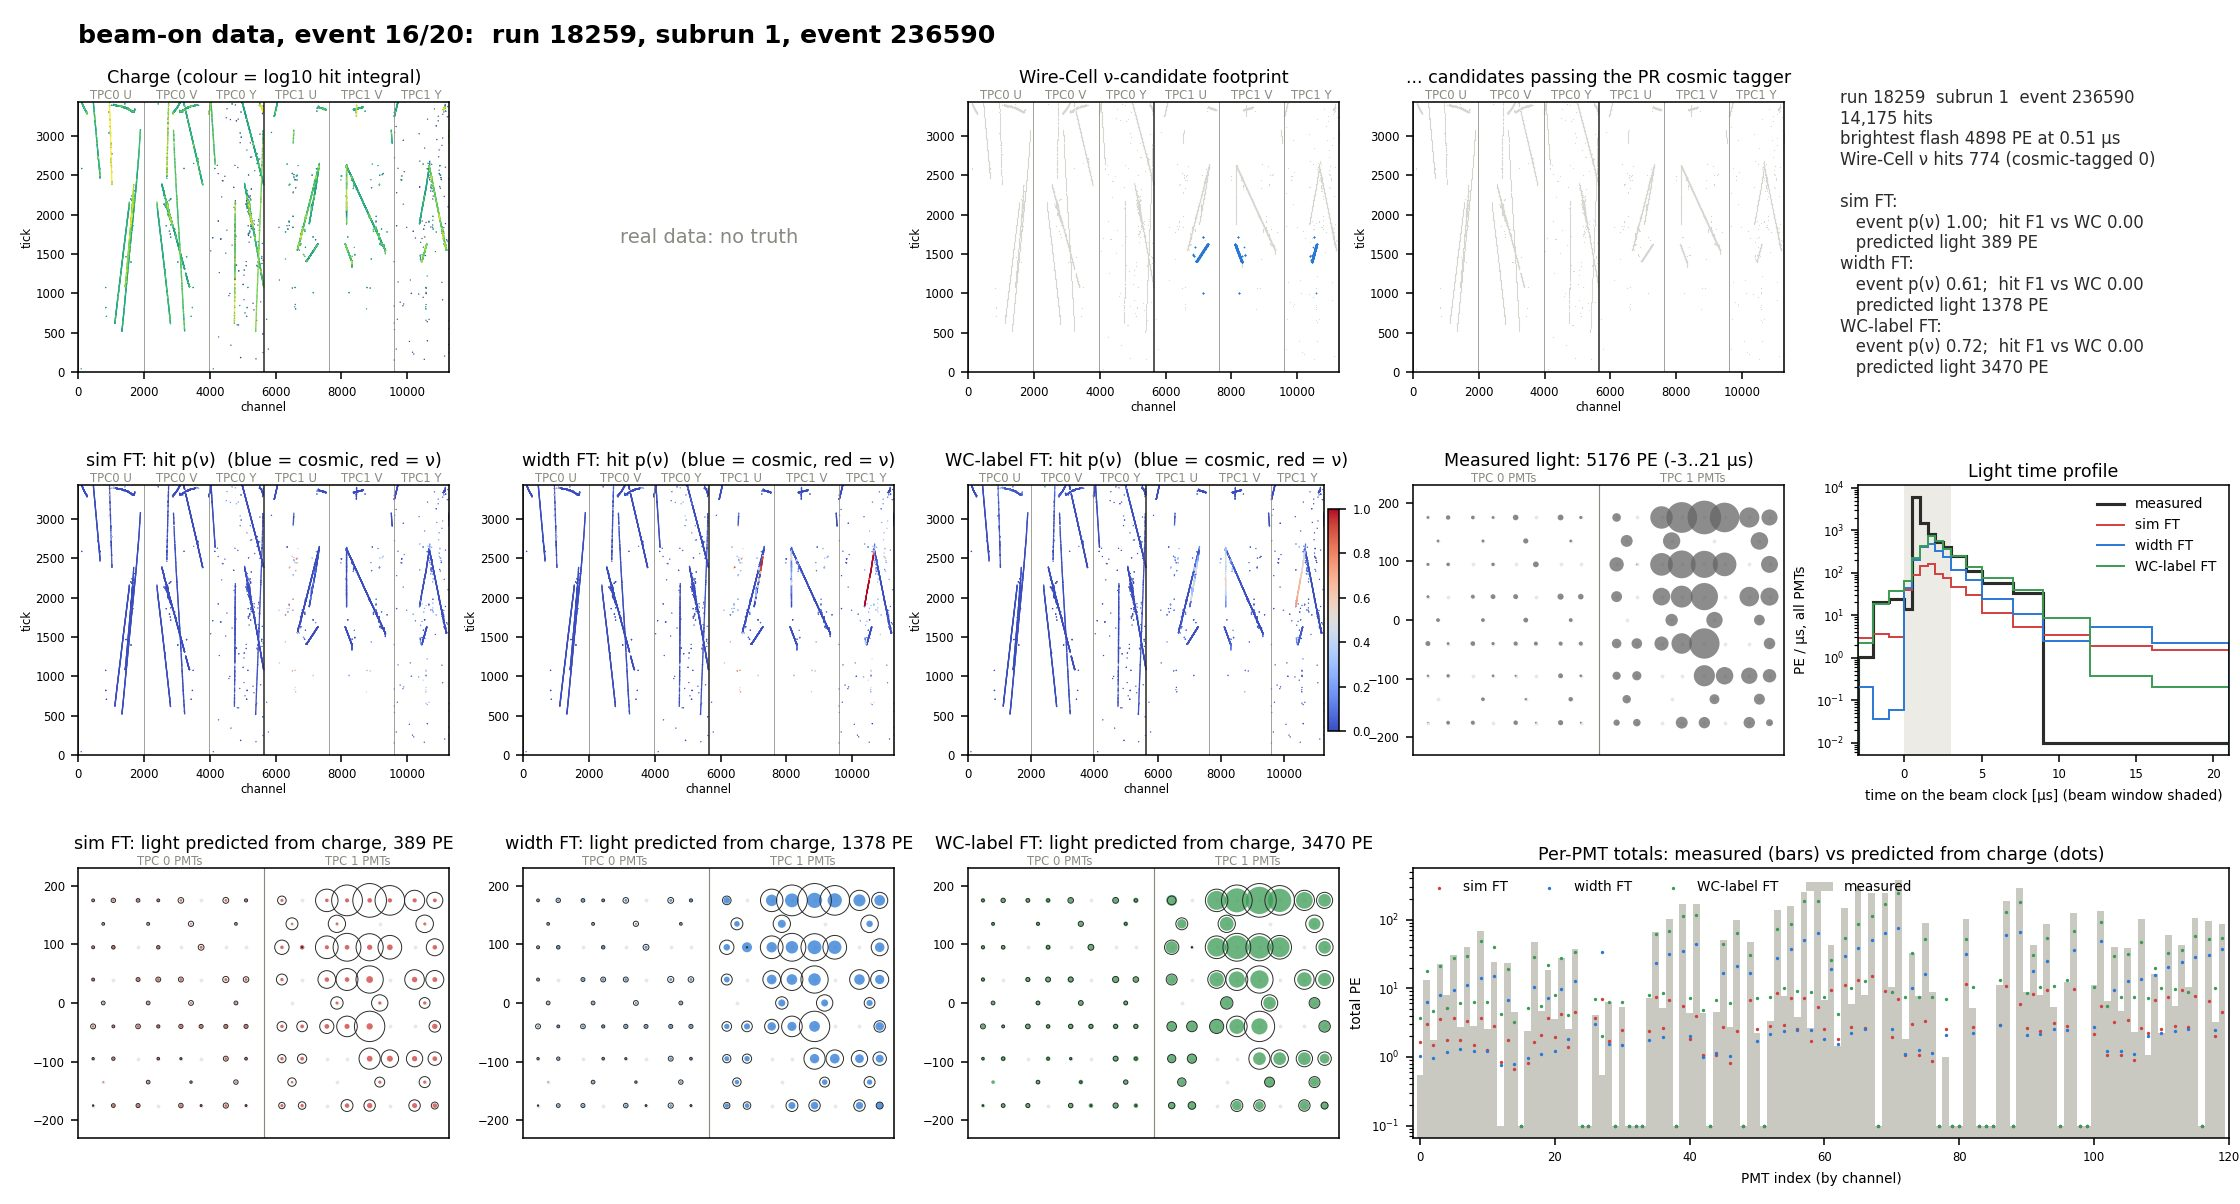
\includegraphics[width=\paperwidth,height=\paperheight,keepaspectratio]{displays/on_15.jpg}}
\end{frame}
% Beam-on data 17/20: run 18255, subrun 1, event 157835; event p(nu): sim FT 0.00, width FT 0.00, WC-label FT 0.62
\begin{frame}[plain]
  \centering\vspace*{-2pt}
  \makebox[\linewidth][c]{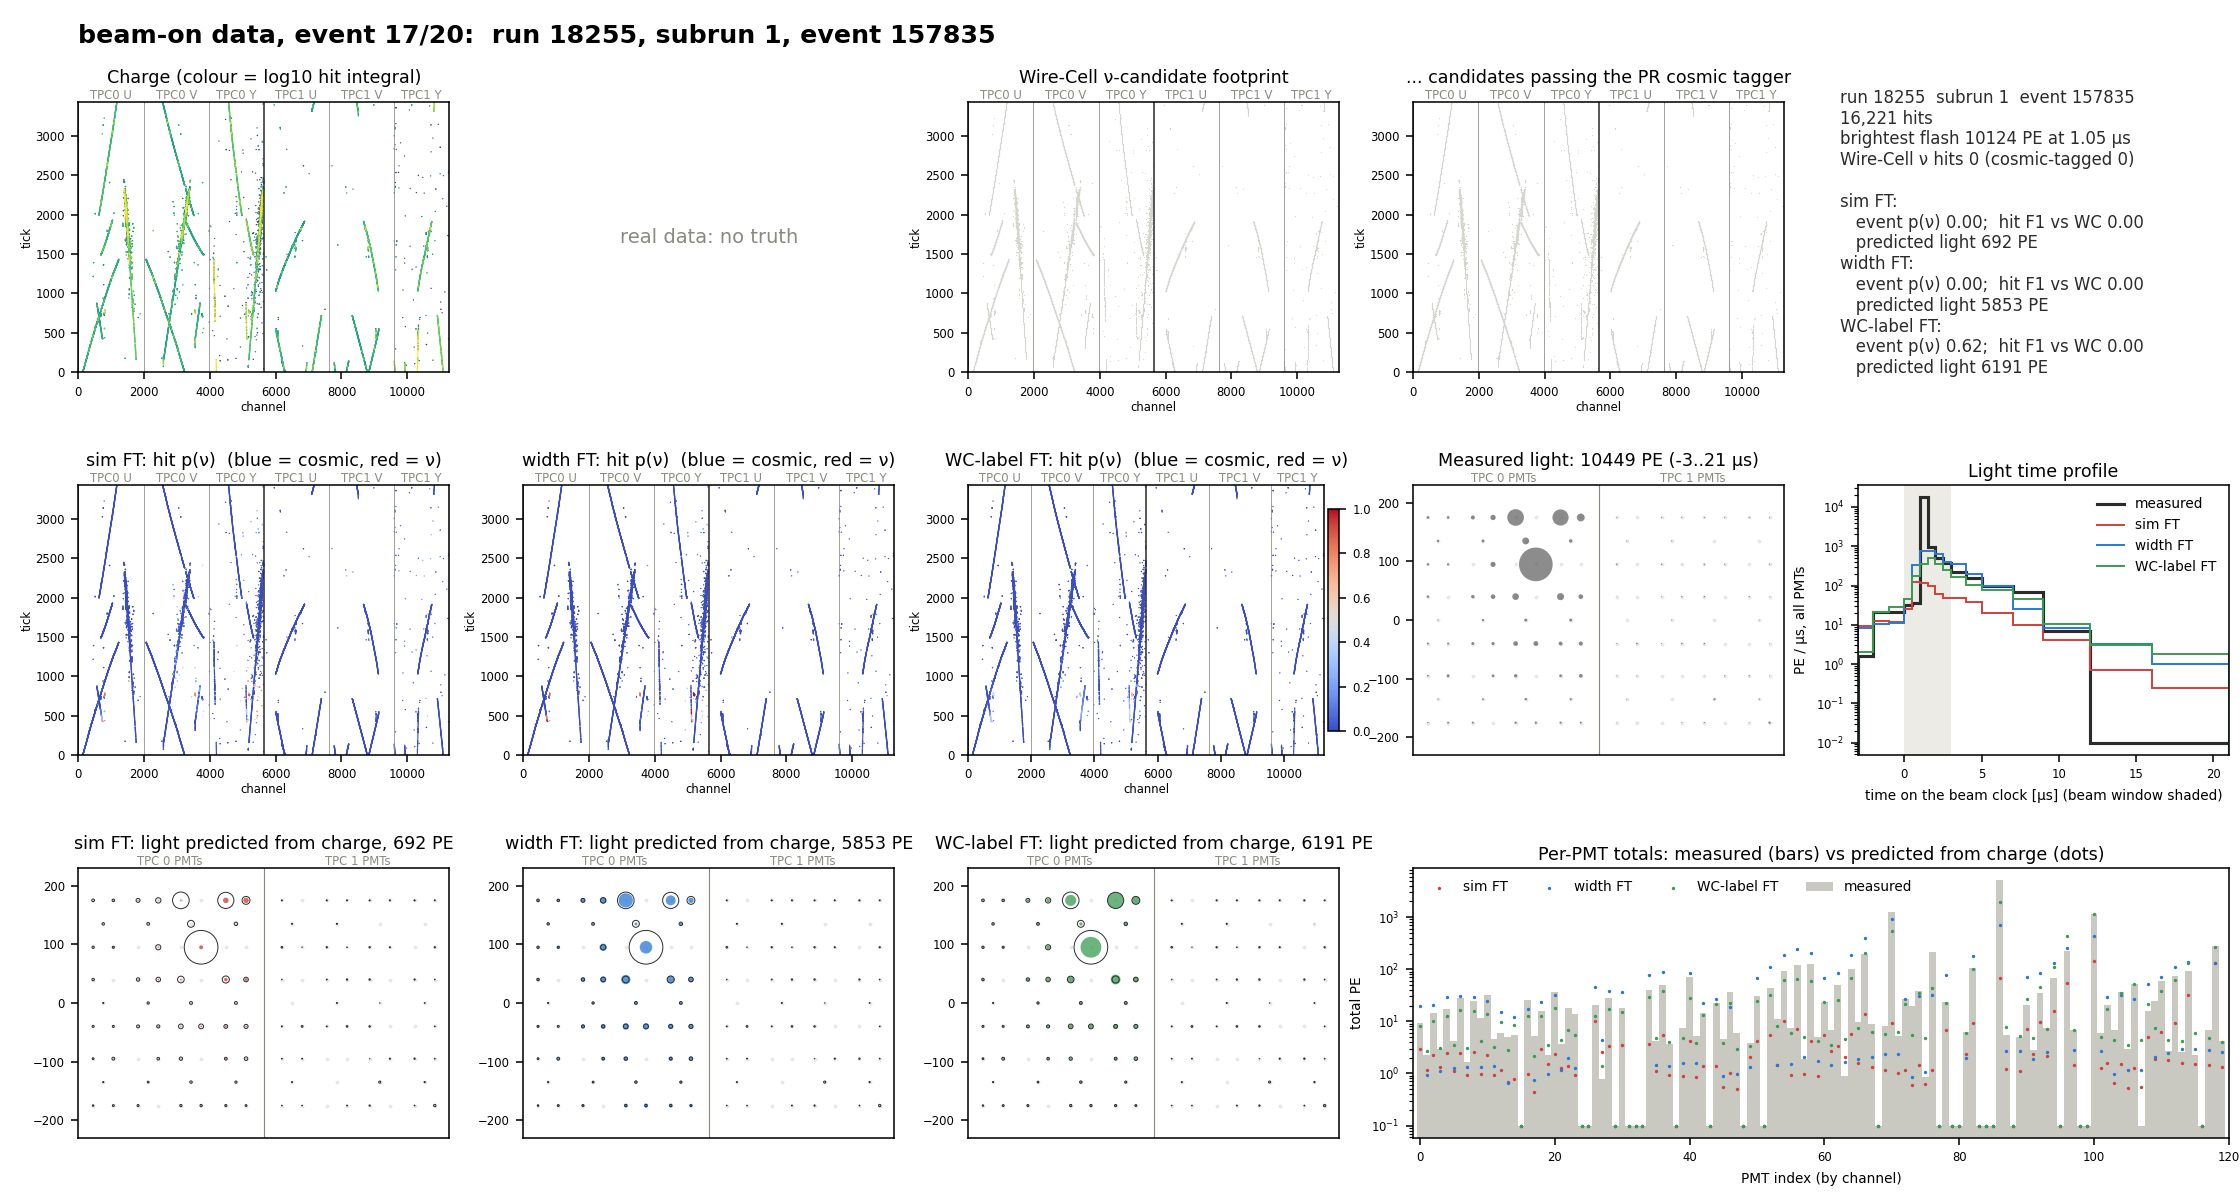
\includegraphics[width=\paperwidth,height=\paperheight,keepaspectratio]{displays/on_16.jpg}}
\end{frame}
% Beam-on data 18/20: run 18255, subrun 1, event 315441; event p(nu): sim FT 1.00, width FT 1.00, WC-label FT 0.88
\begin{frame}[plain]
  \centering\vspace*{-2pt}
  \makebox[\linewidth][c]{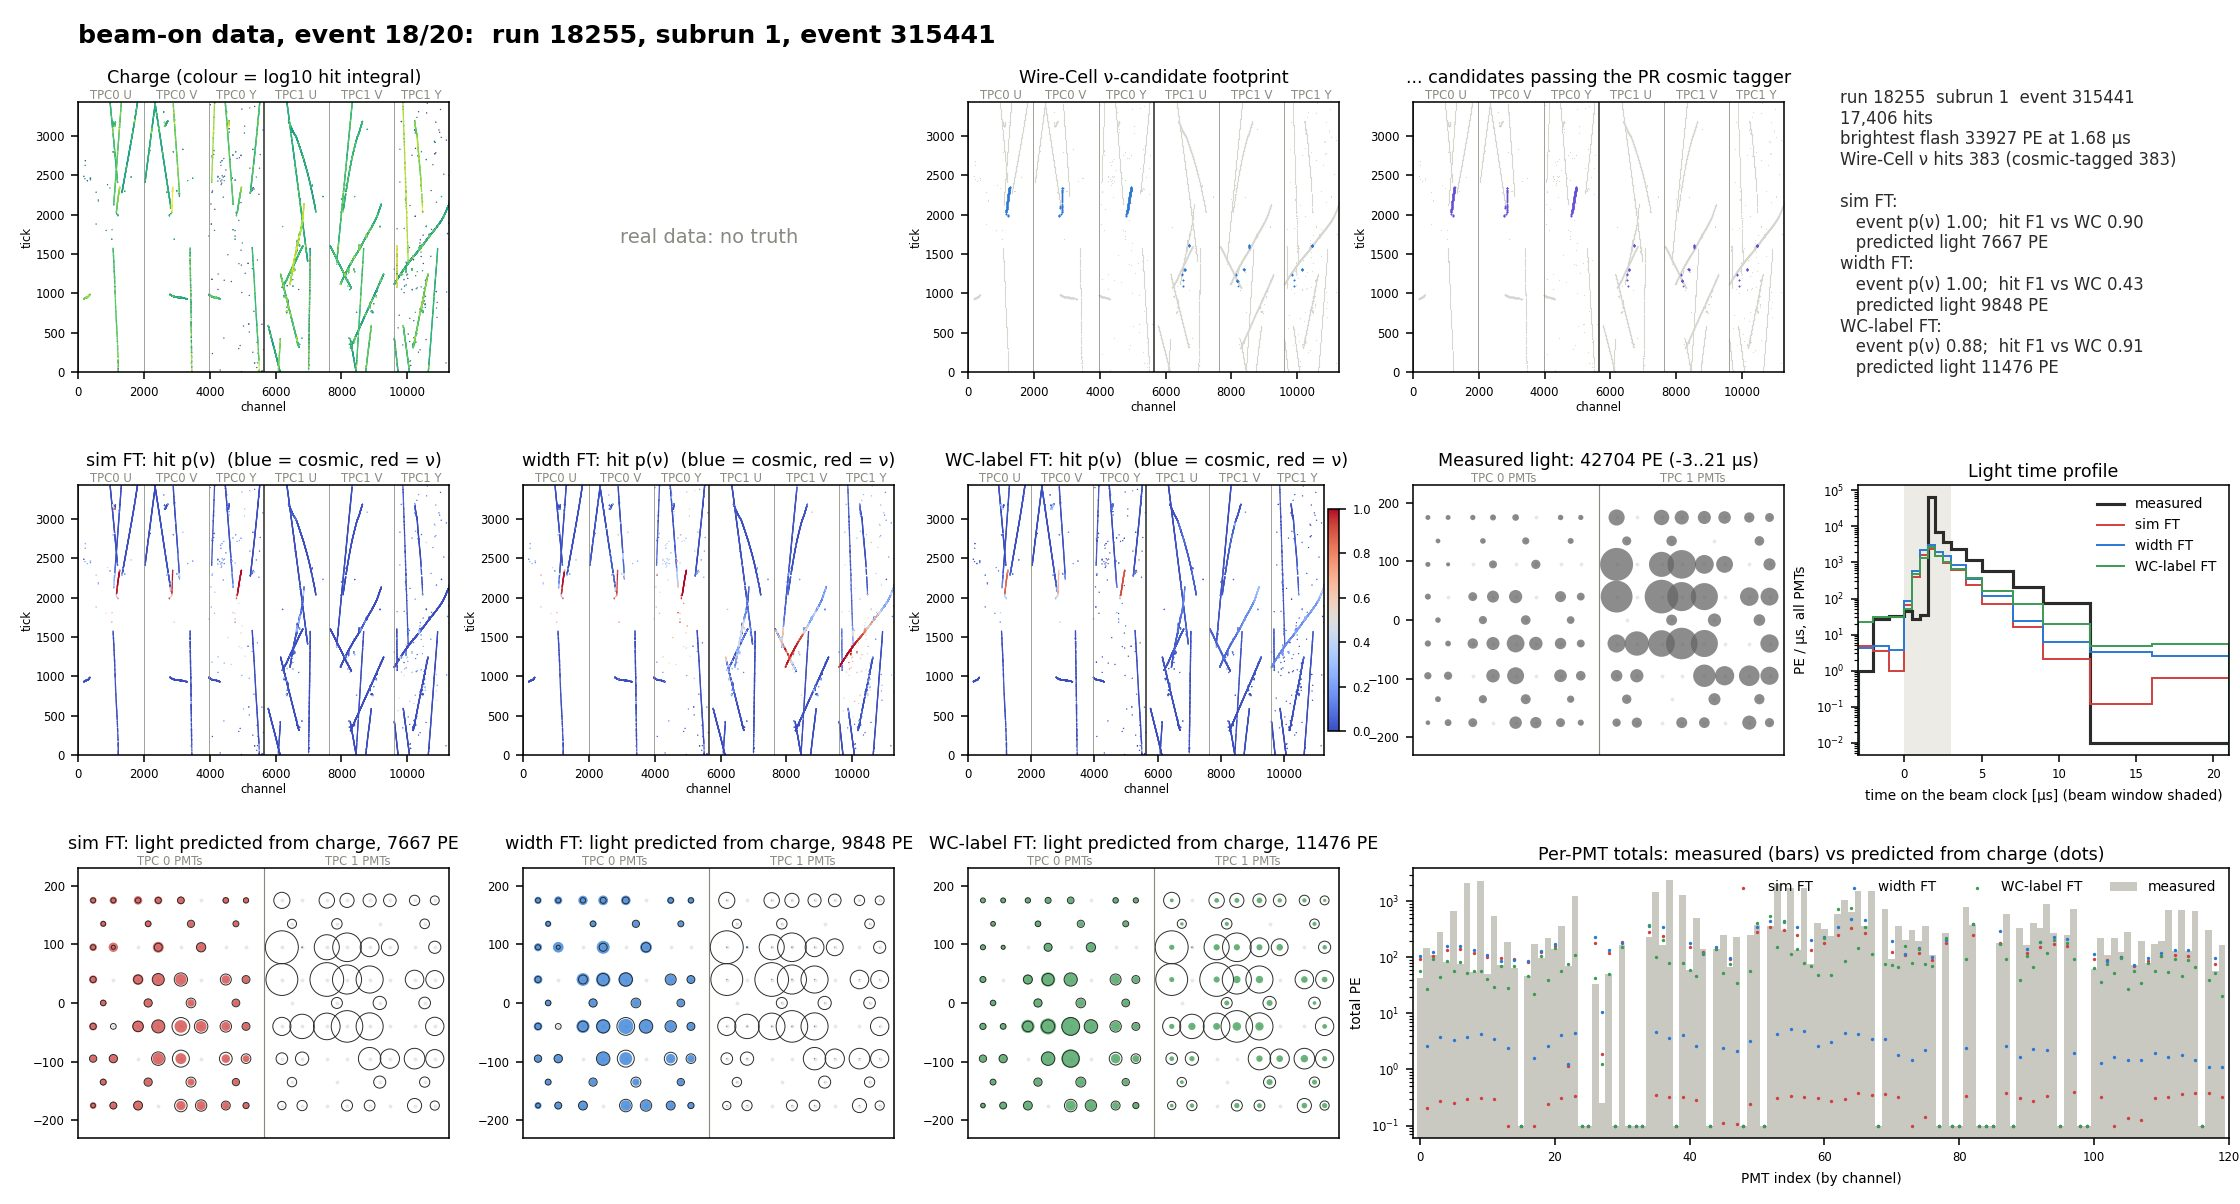
\includegraphics[width=\paperwidth,height=\paperheight,keepaspectratio]{displays/on_17.jpg}}
\end{frame}
% Beam-on data 19/20: run 18259, subrun 1, event 138755; event p(nu): sim FT 1.00, width FT 1.00, WC-label FT 0.98
\begin{frame}[plain]
  \centering\vspace*{-2pt}
  \makebox[\linewidth][c]{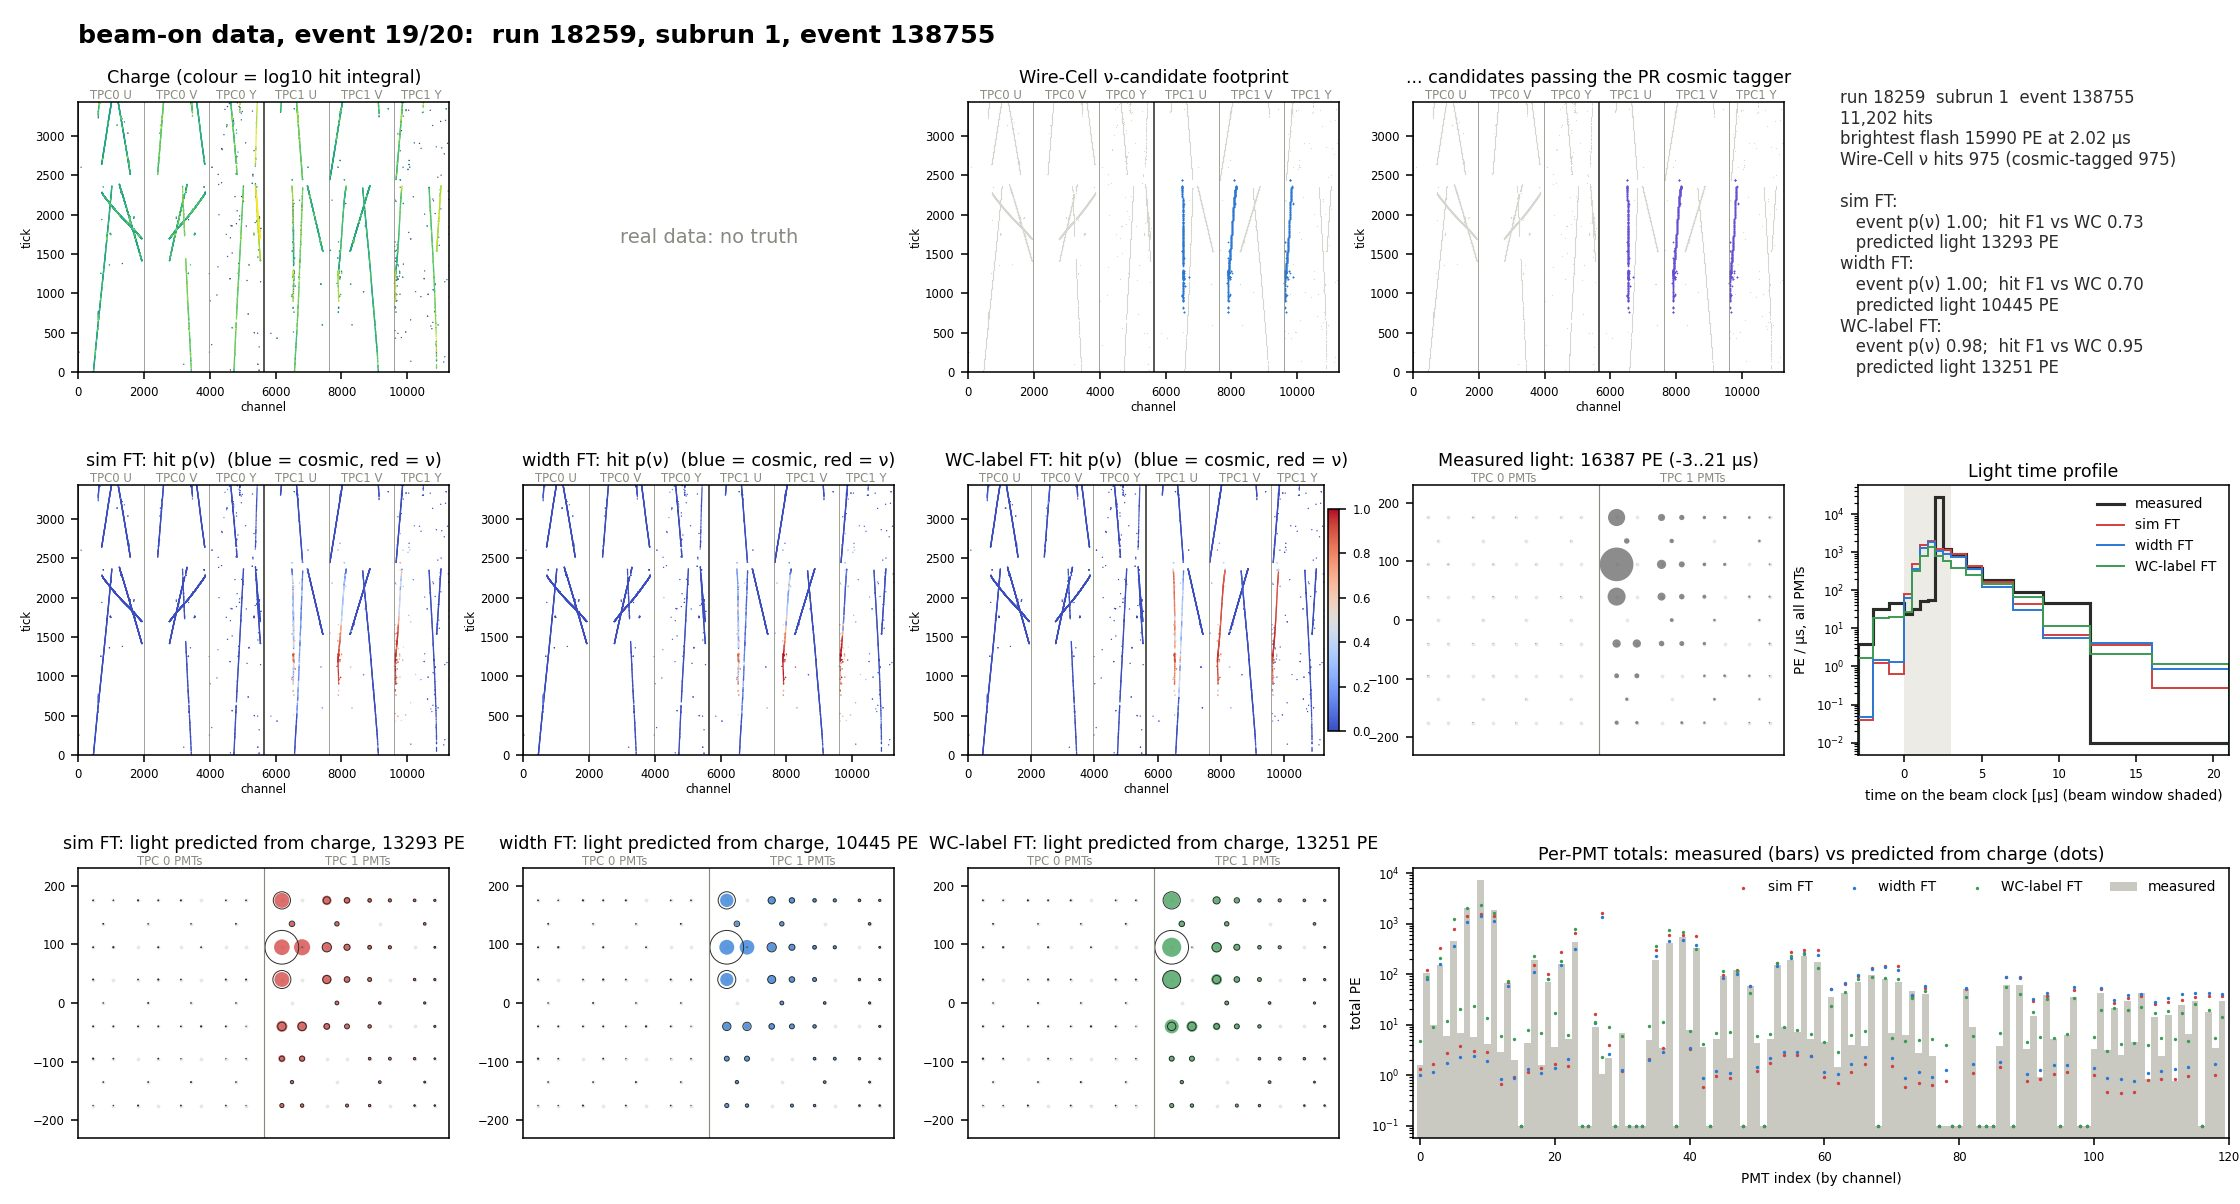
\includegraphics[width=\paperwidth,height=\paperheight,keepaspectratio]{displays/on_18.jpg}}
\end{frame}
% Beam-on data 20/20: run 18255, subrun 1, event 24654; event p(nu): sim FT 1.00, width FT 1.00, WC-label FT 0.97
\begin{frame}[plain]
  \centering\vspace*{-2pt}
  \makebox[\linewidth][c]{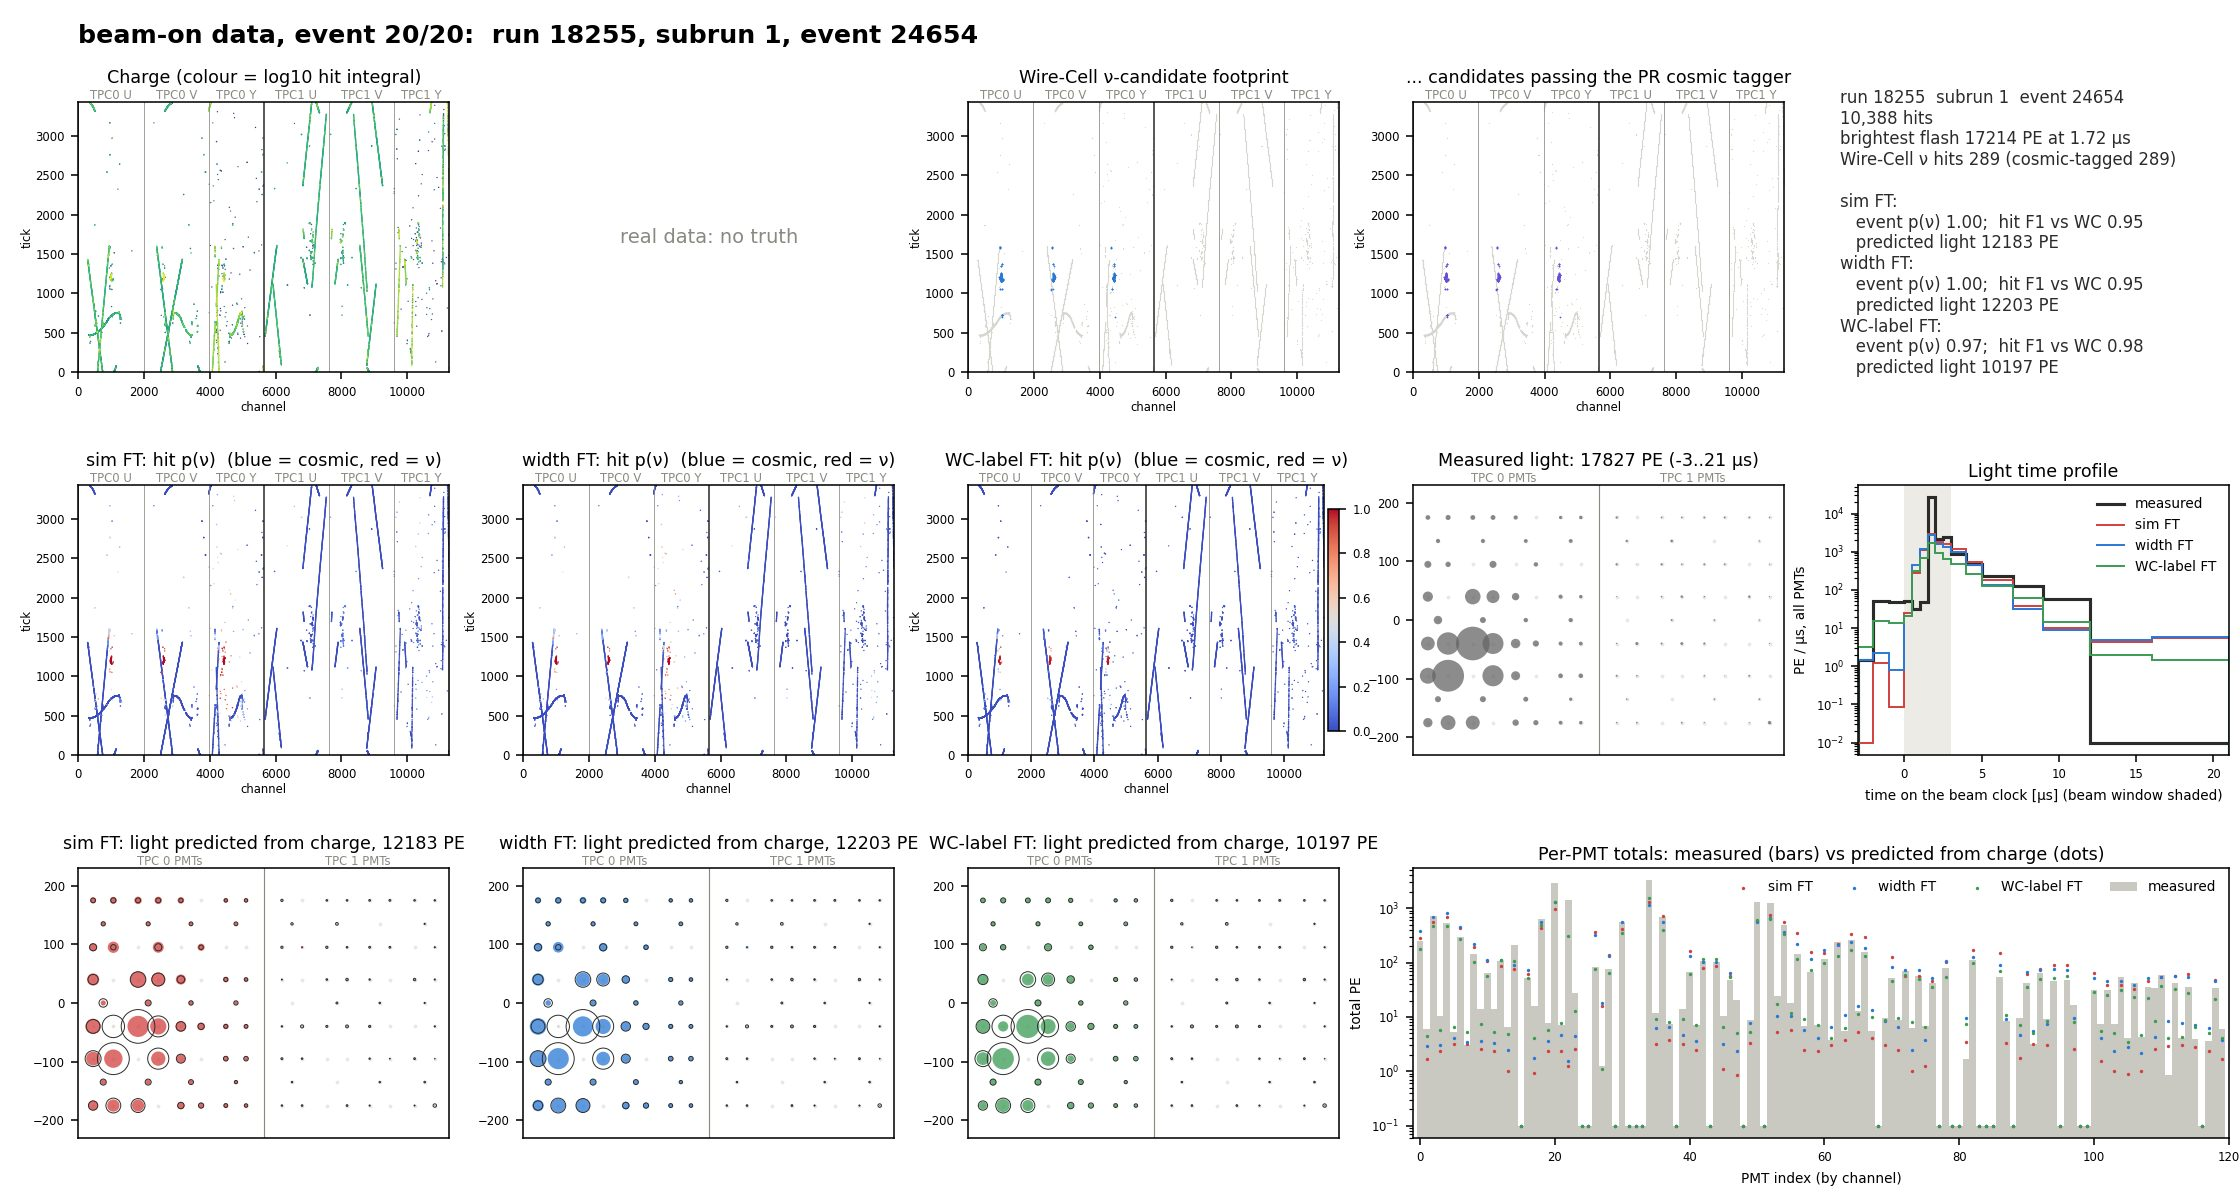
\includegraphics[width=\paperwidth,height=\paperheight,keepaspectratio]{displays/on_19.jpg}}
\end{frame}
\subsection{Off-beam data}
% Off-beam data 1/20: run 18329, subrun 1, event 56813; event p(nu): sim FT 0.00, width FT 0.00, WC-label FT 0.00
\begin{frame}[plain]
  \centering\vspace*{-2pt}
  \makebox[\linewidth][c]{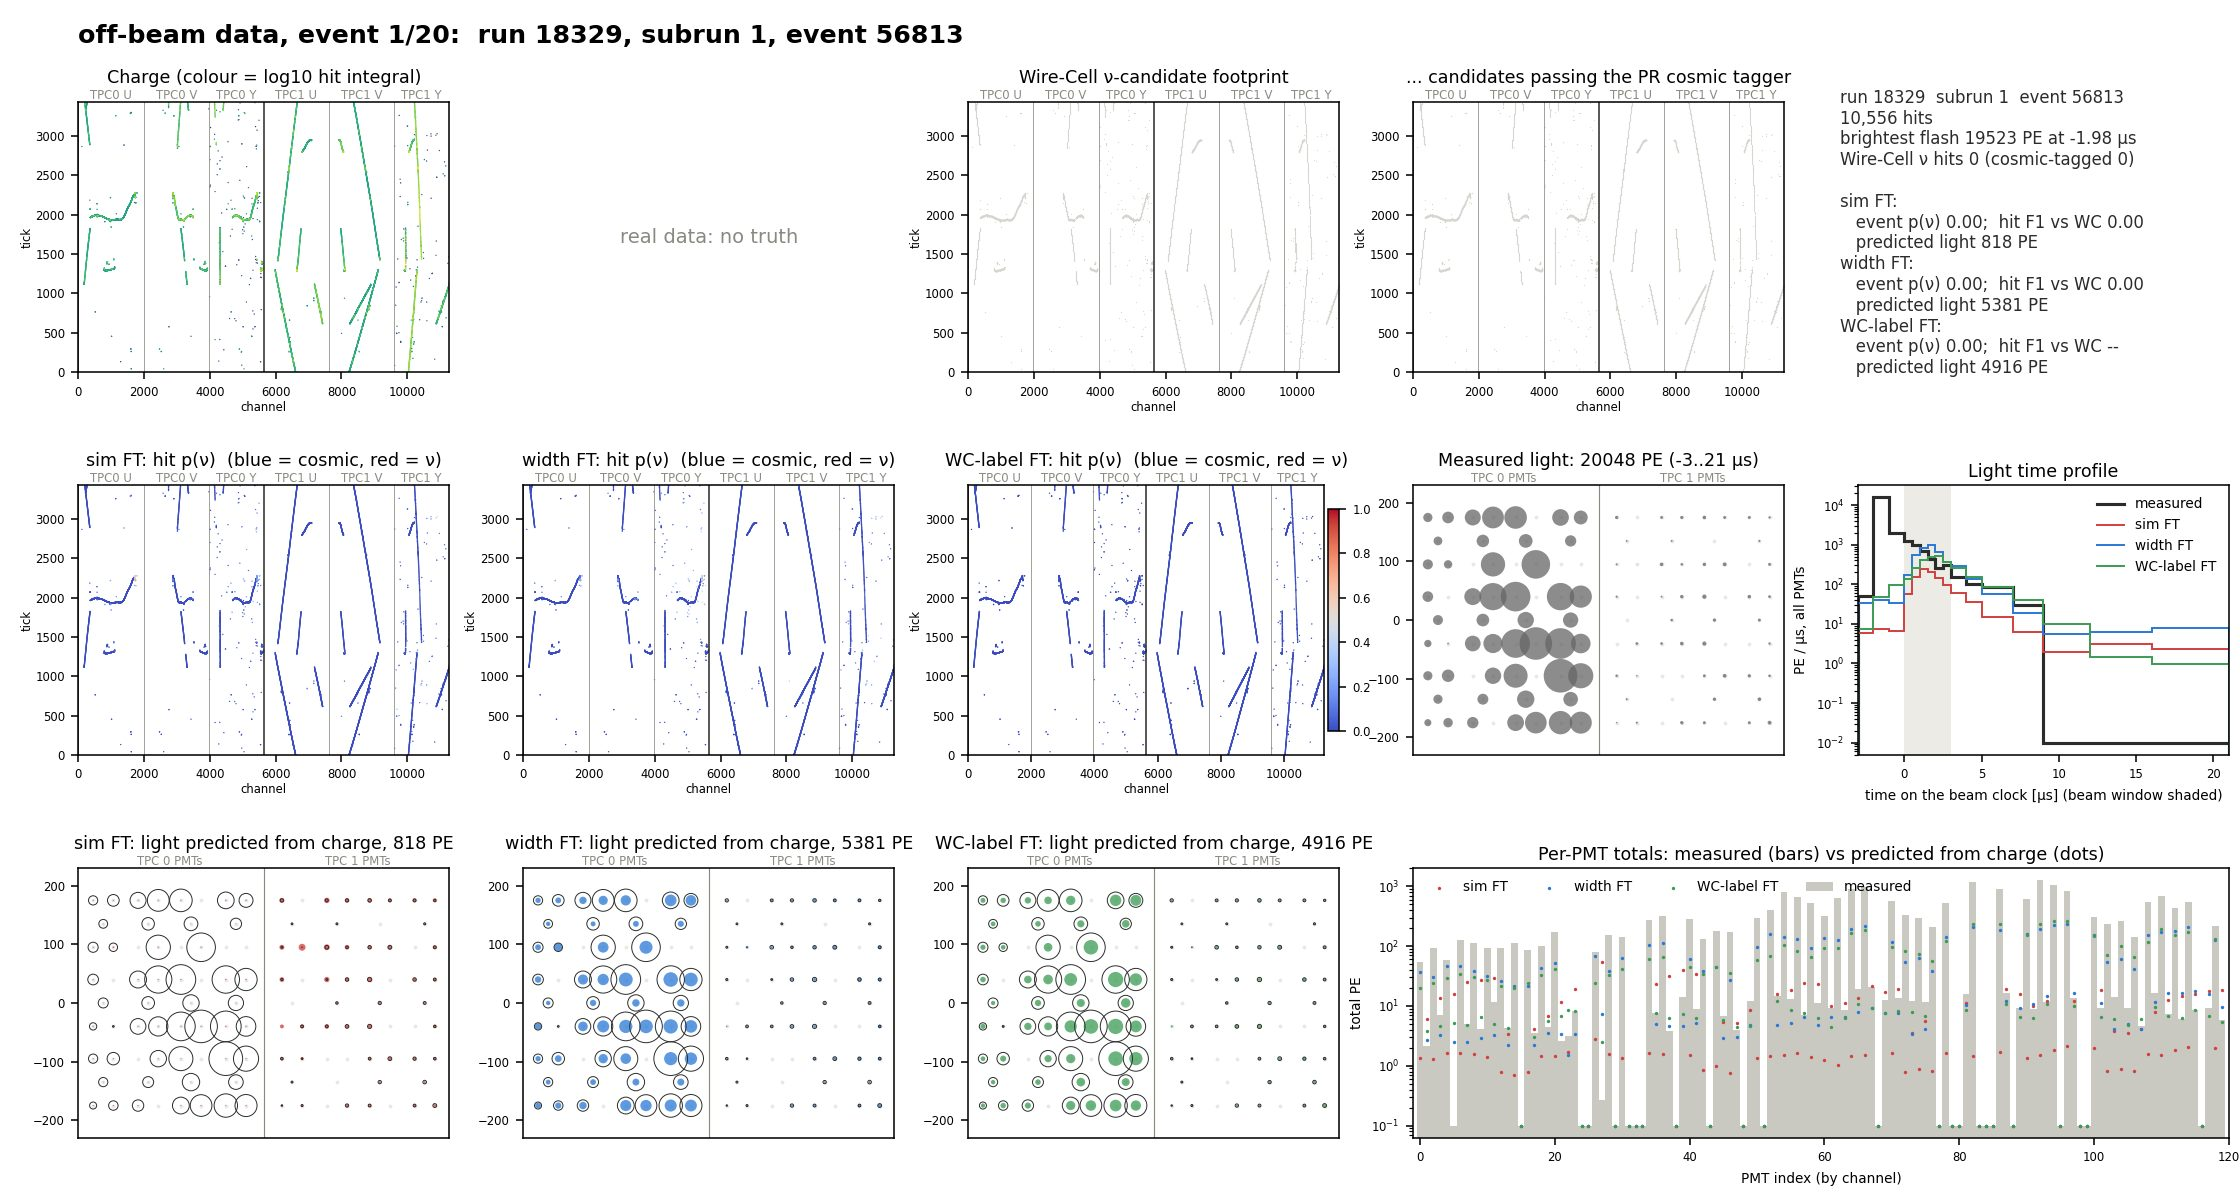
\includegraphics[width=\paperwidth,height=\paperheight,keepaspectratio]{displays/off_00.jpg}}
\end{frame}
% Off-beam data 2/20: run 18355, subrun 1, event 399079; event p(nu): sim FT 0.00, width FT 0.00, WC-label FT 0.00
\begin{frame}[plain]
  \centering\vspace*{-2pt}
  \makebox[\linewidth][c]{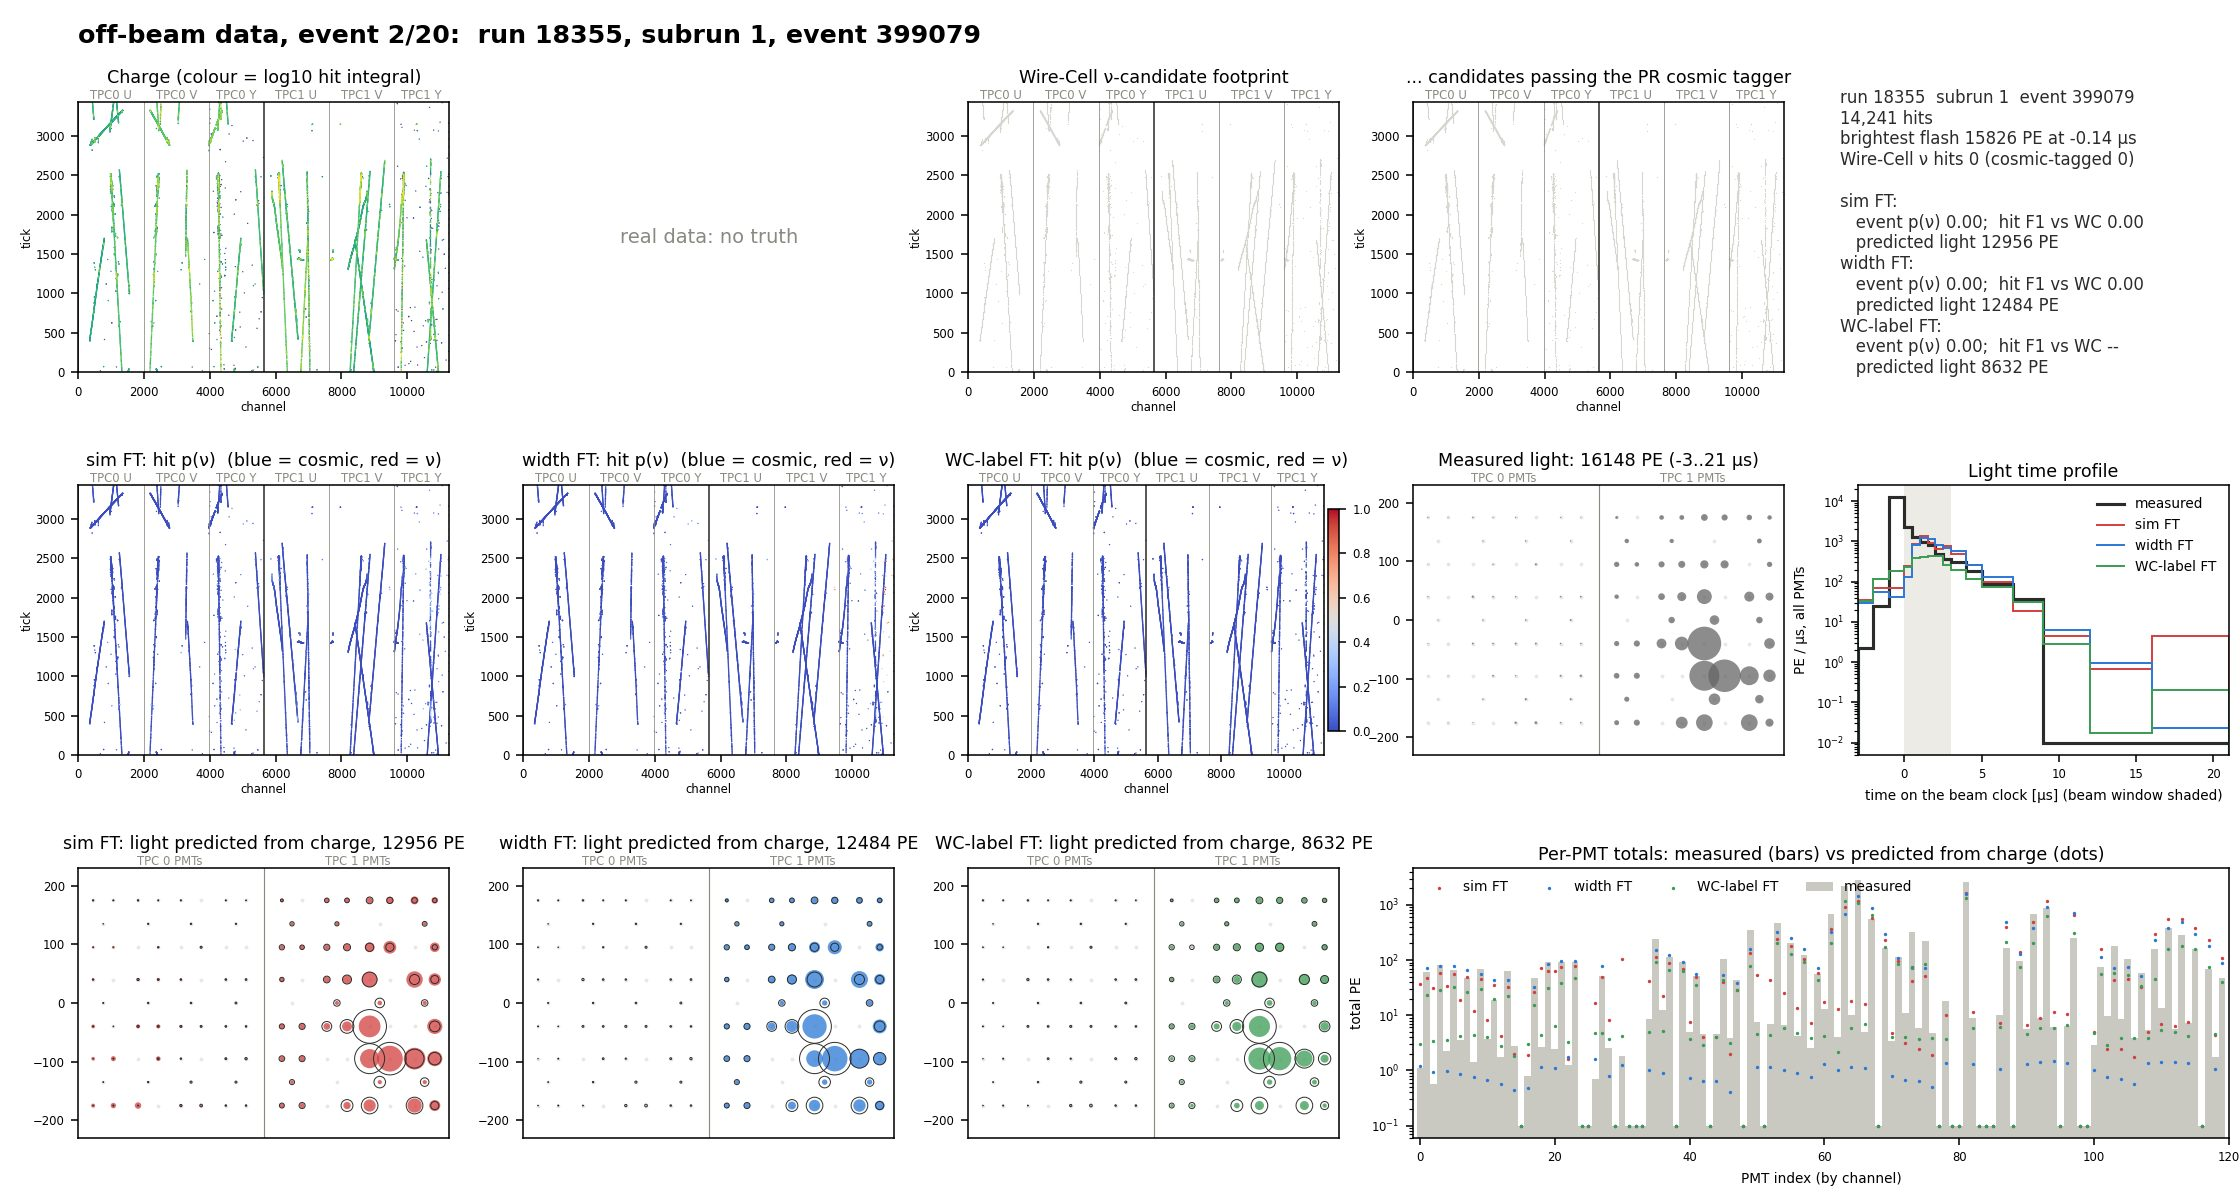
\includegraphics[width=\paperwidth,height=\paperheight,keepaspectratio]{displays/off_01.jpg}}
\end{frame}
% Off-beam data 3/20: run 18468, subrun 1, event 292429; event p(nu): sim FT 0.00, width FT 0.00, WC-label FT 0.12
\begin{frame}[plain]
  \centering\vspace*{-2pt}
  \makebox[\linewidth][c]{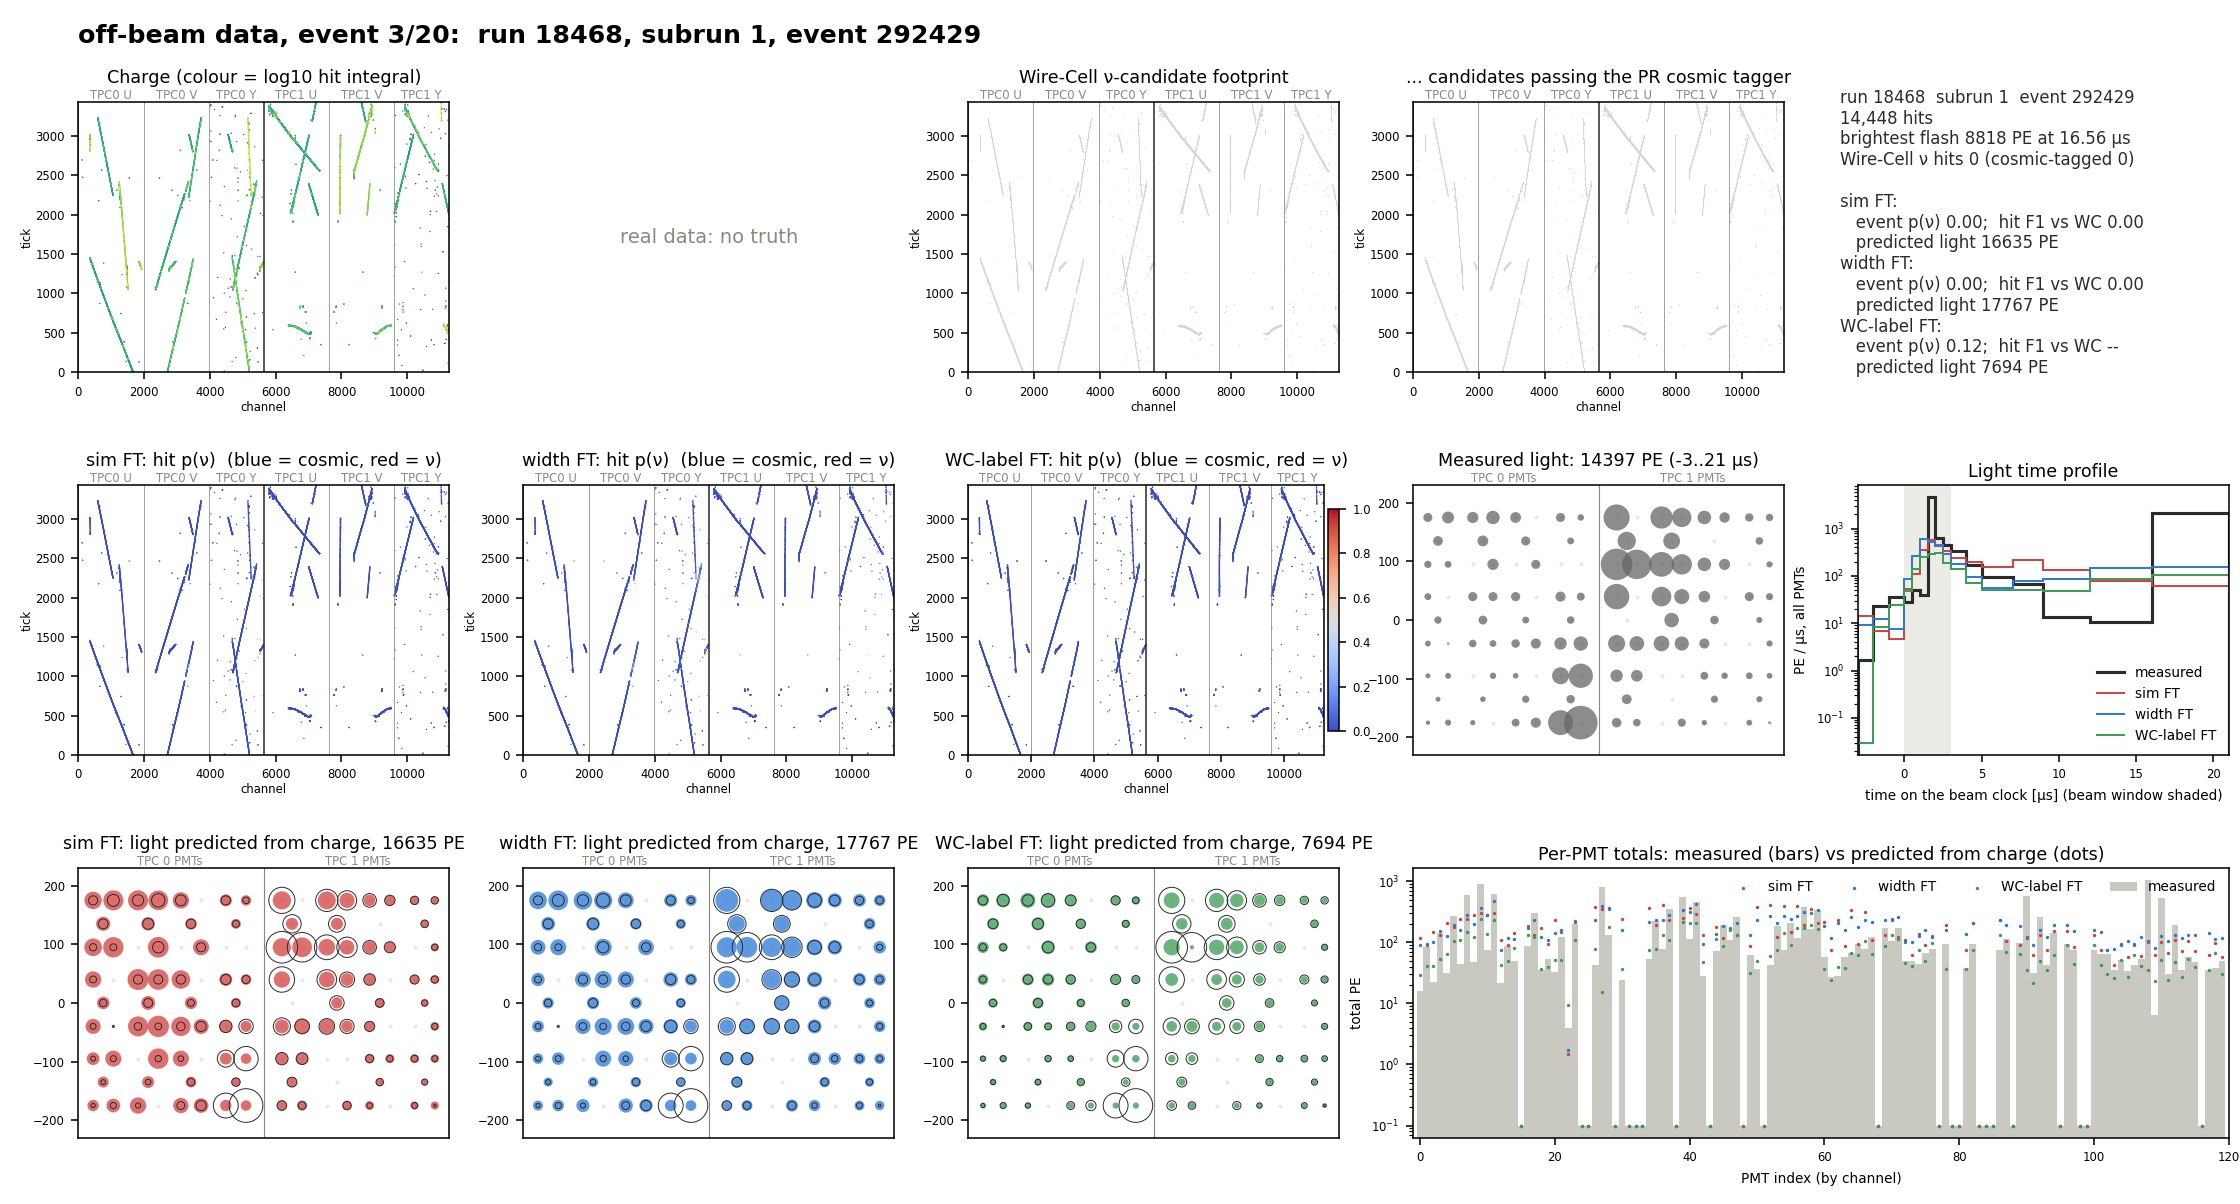
\includegraphics[width=\paperwidth,height=\paperheight,keepaspectratio]{displays/off_02.jpg}}
\end{frame}
% Off-beam data 4/20: run 18275, subrun 1, event 7671; event p(nu): sim FT 0.00, width FT 0.00, WC-label FT 0.03
\begin{frame}[plain]
  \centering\vspace*{-2pt}
  \makebox[\linewidth][c]{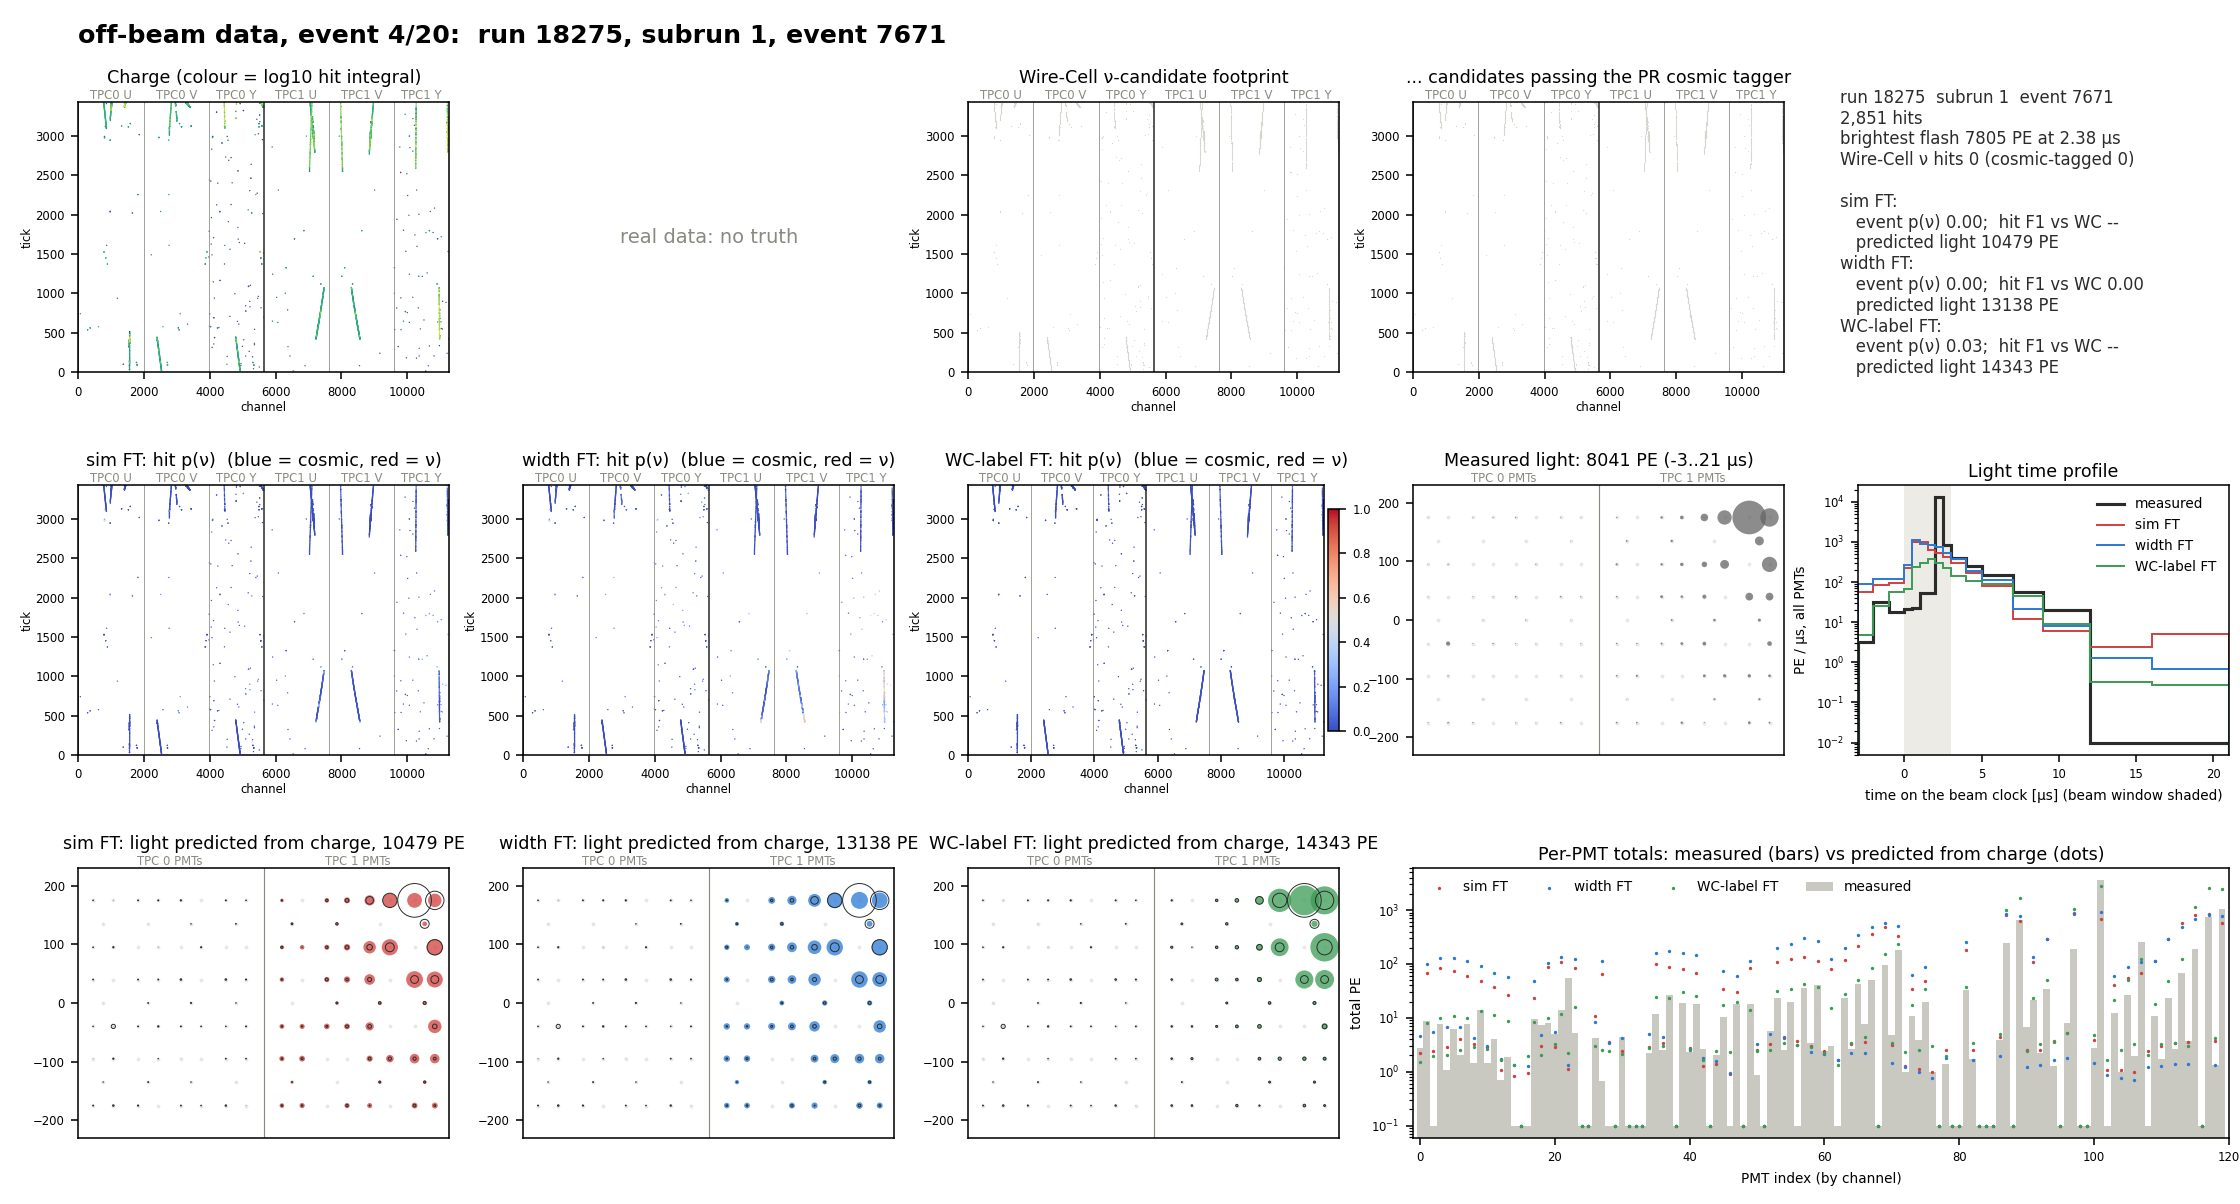
\includegraphics[width=\paperwidth,height=\paperheight,keepaspectratio]{displays/off_03.jpg}}
\end{frame}
% Off-beam data 5/20: run 18484, subrun 1, event 270322; event p(nu): sim FT 0.00, width FT 0.00, WC-label FT 0.00
\begin{frame}[plain]
  \centering\vspace*{-2pt}
  \makebox[\linewidth][c]{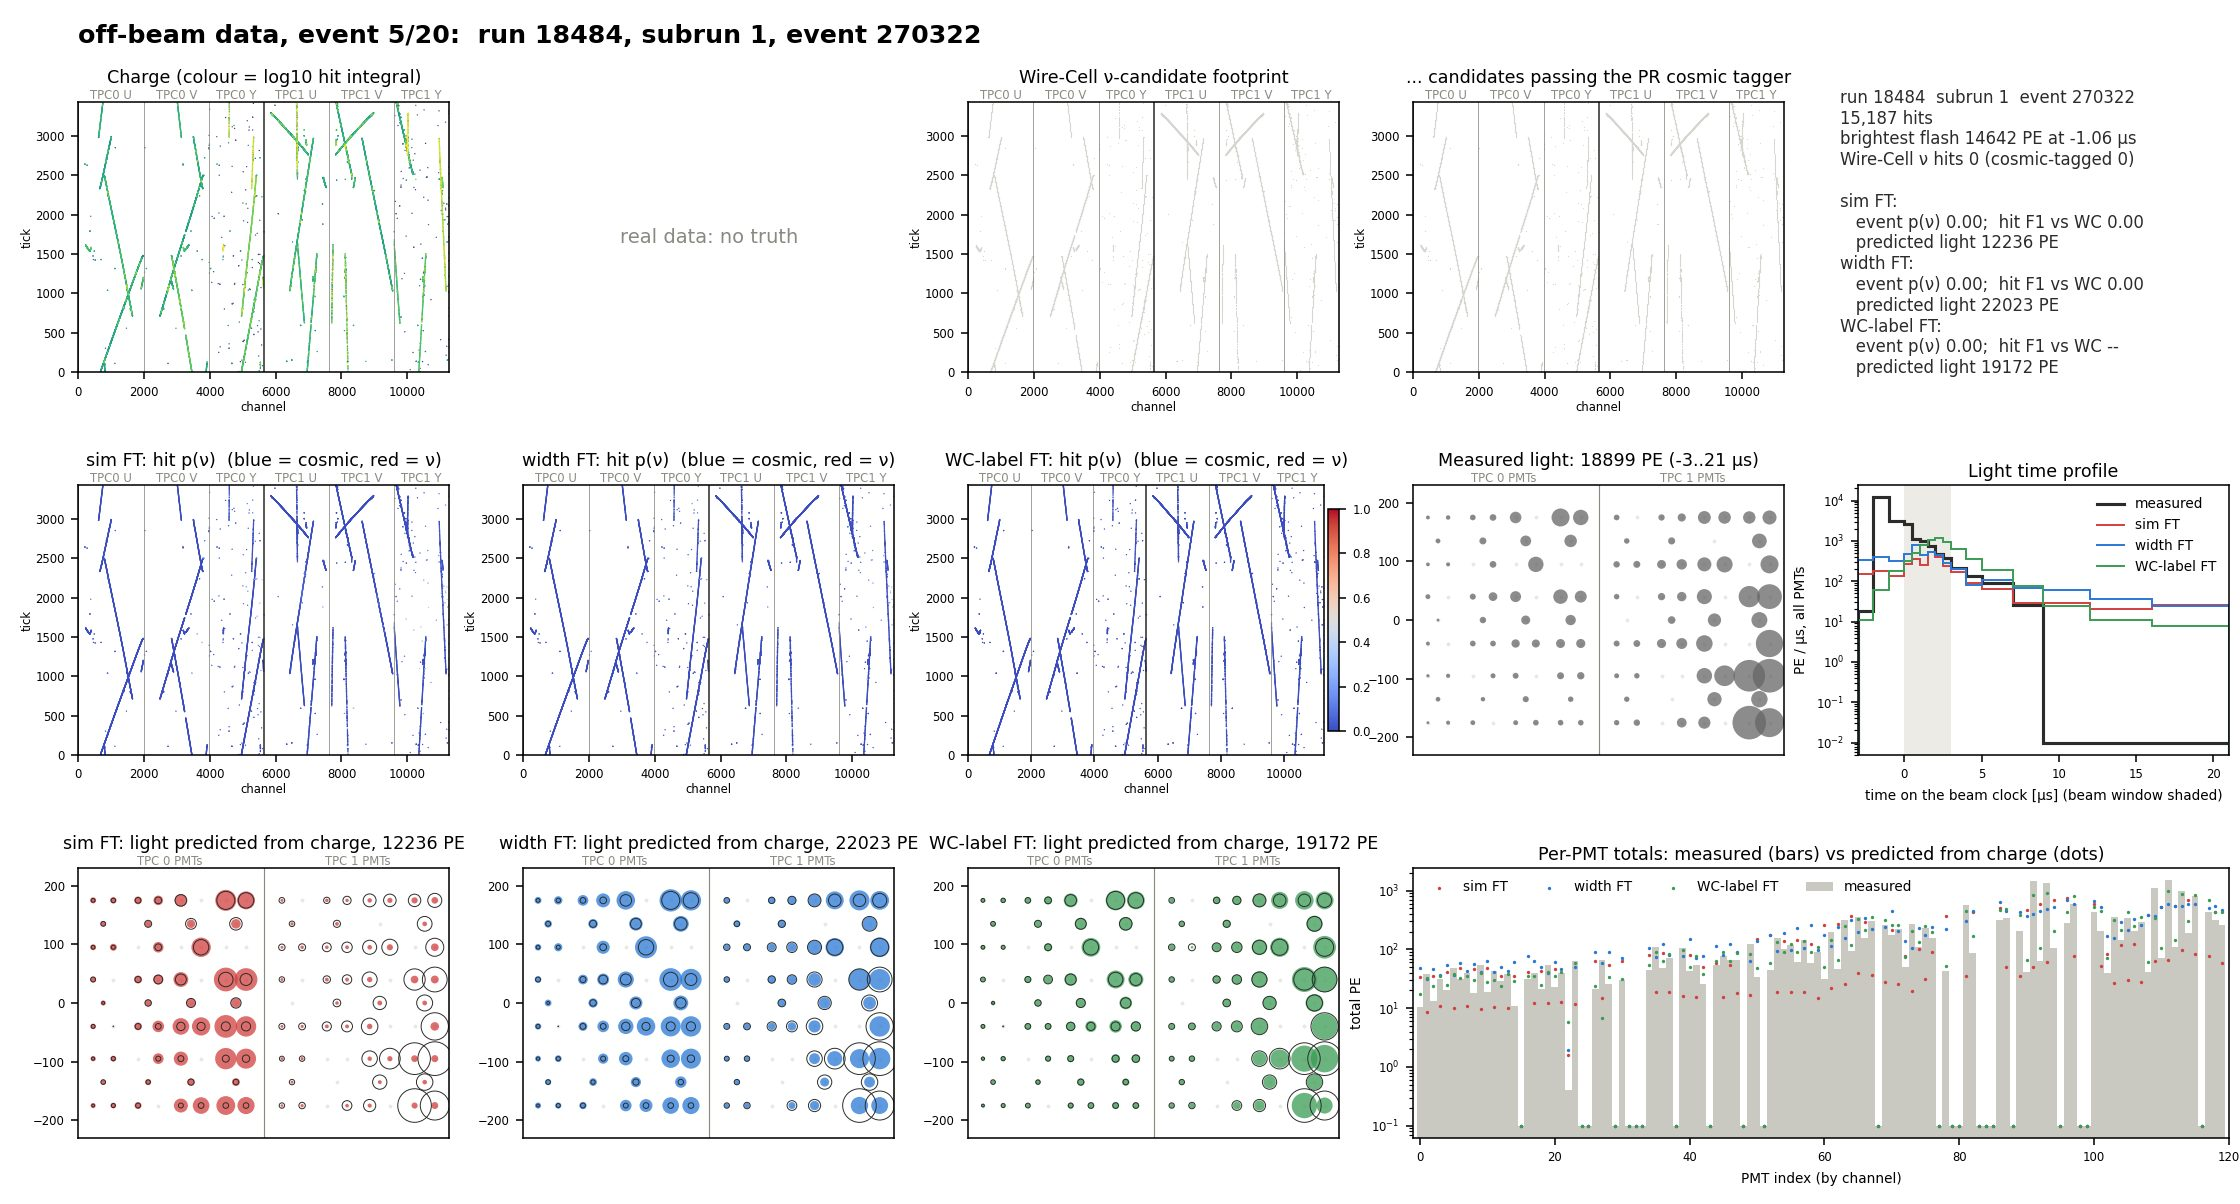
\includegraphics[width=\paperwidth,height=\paperheight,keepaspectratio]{displays/off_04.jpg}}
\end{frame}
% Off-beam data 6/20: run 18308, subrun 1, event 54357; event p(nu): sim FT 0.00, width FT 0.00, WC-label FT 0.00
\begin{frame}[plain]
  \centering\vspace*{-2pt}
  \makebox[\linewidth][c]{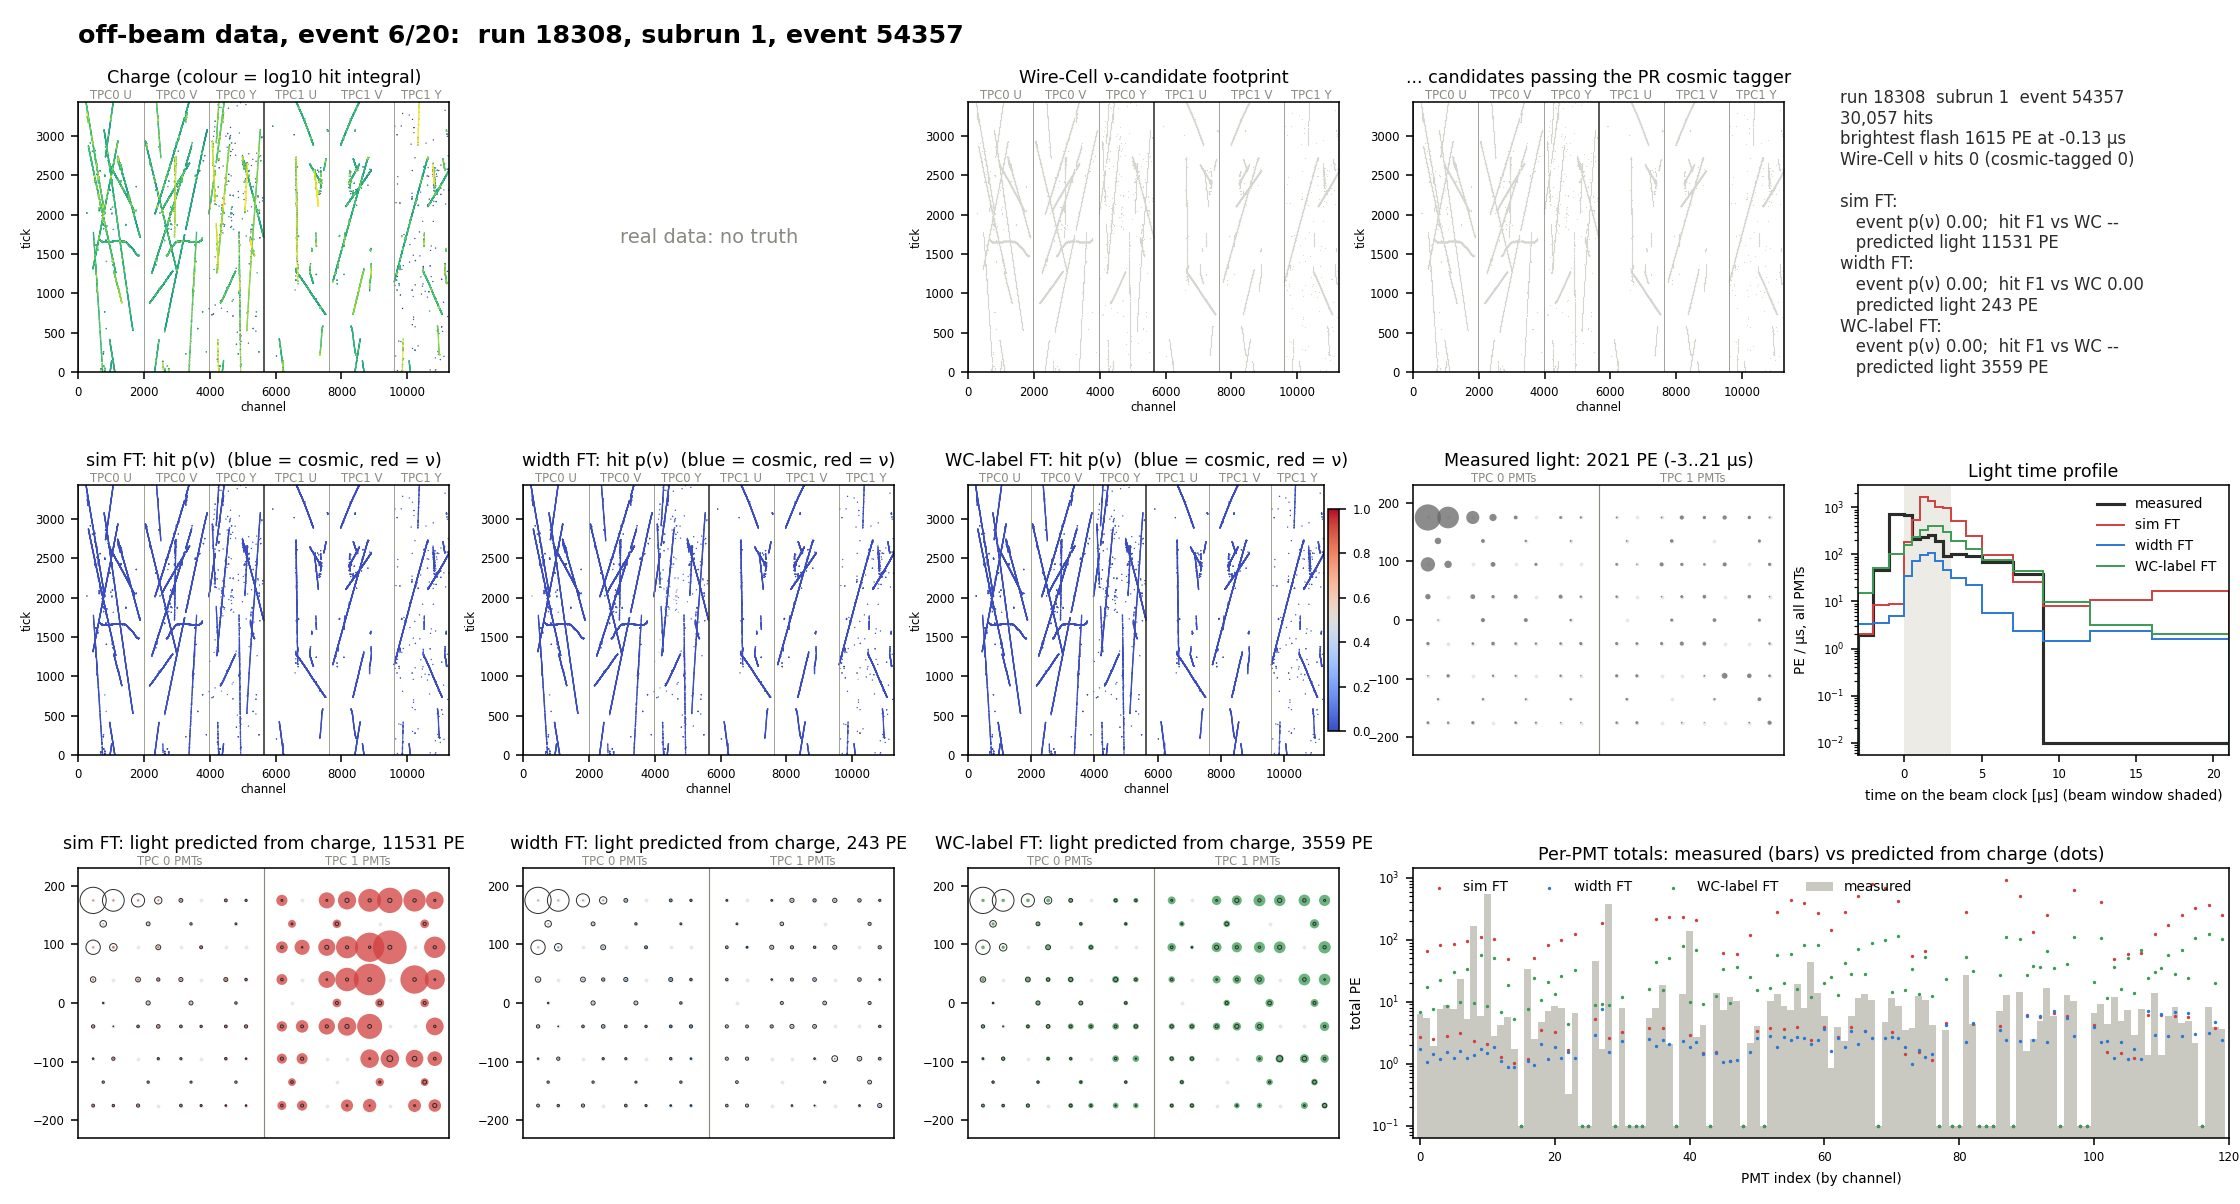
\includegraphics[width=\paperwidth,height=\paperheight,keepaspectratio]{displays/off_05.jpg}}
\end{frame}
% Off-beam data 7/20: run 18329, subrun 1, event 439641; event p(nu): sim FT 0.11, width FT 0.00, WC-label FT 0.03
\begin{frame}[plain]
  \centering\vspace*{-2pt}
  \makebox[\linewidth][c]{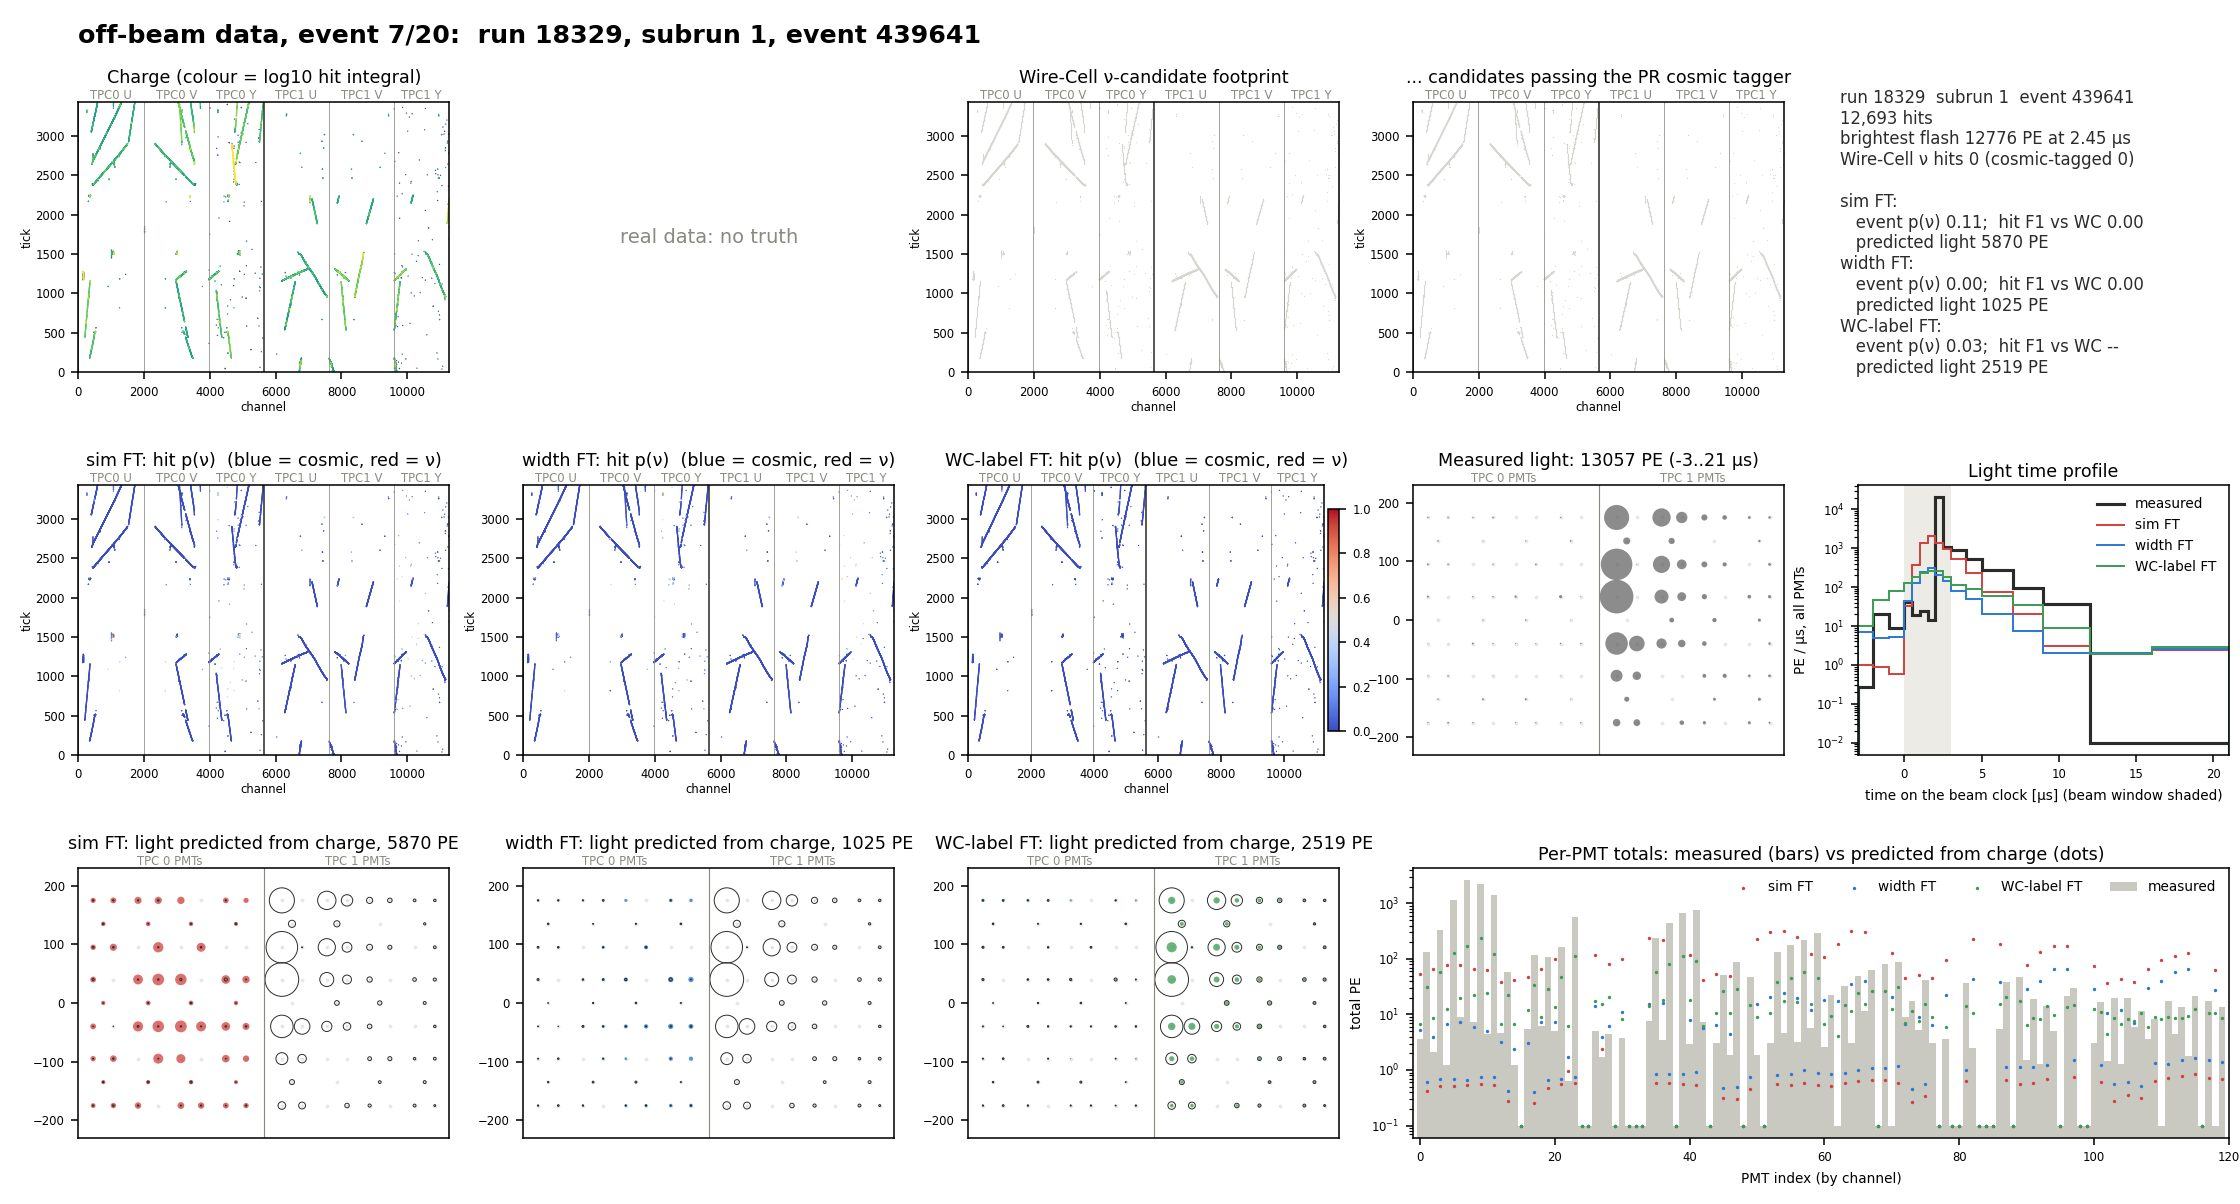
\includegraphics[width=\paperwidth,height=\paperheight,keepaspectratio]{displays/off_06.jpg}}
\end{frame}
% Off-beam data 8/20: run 18250, subrun 1, event 102489; event p(nu): sim FT 0.00, width FT 0.00, WC-label FT 0.03
\begin{frame}[plain]
  \centering\vspace*{-2pt}
  \makebox[\linewidth][c]{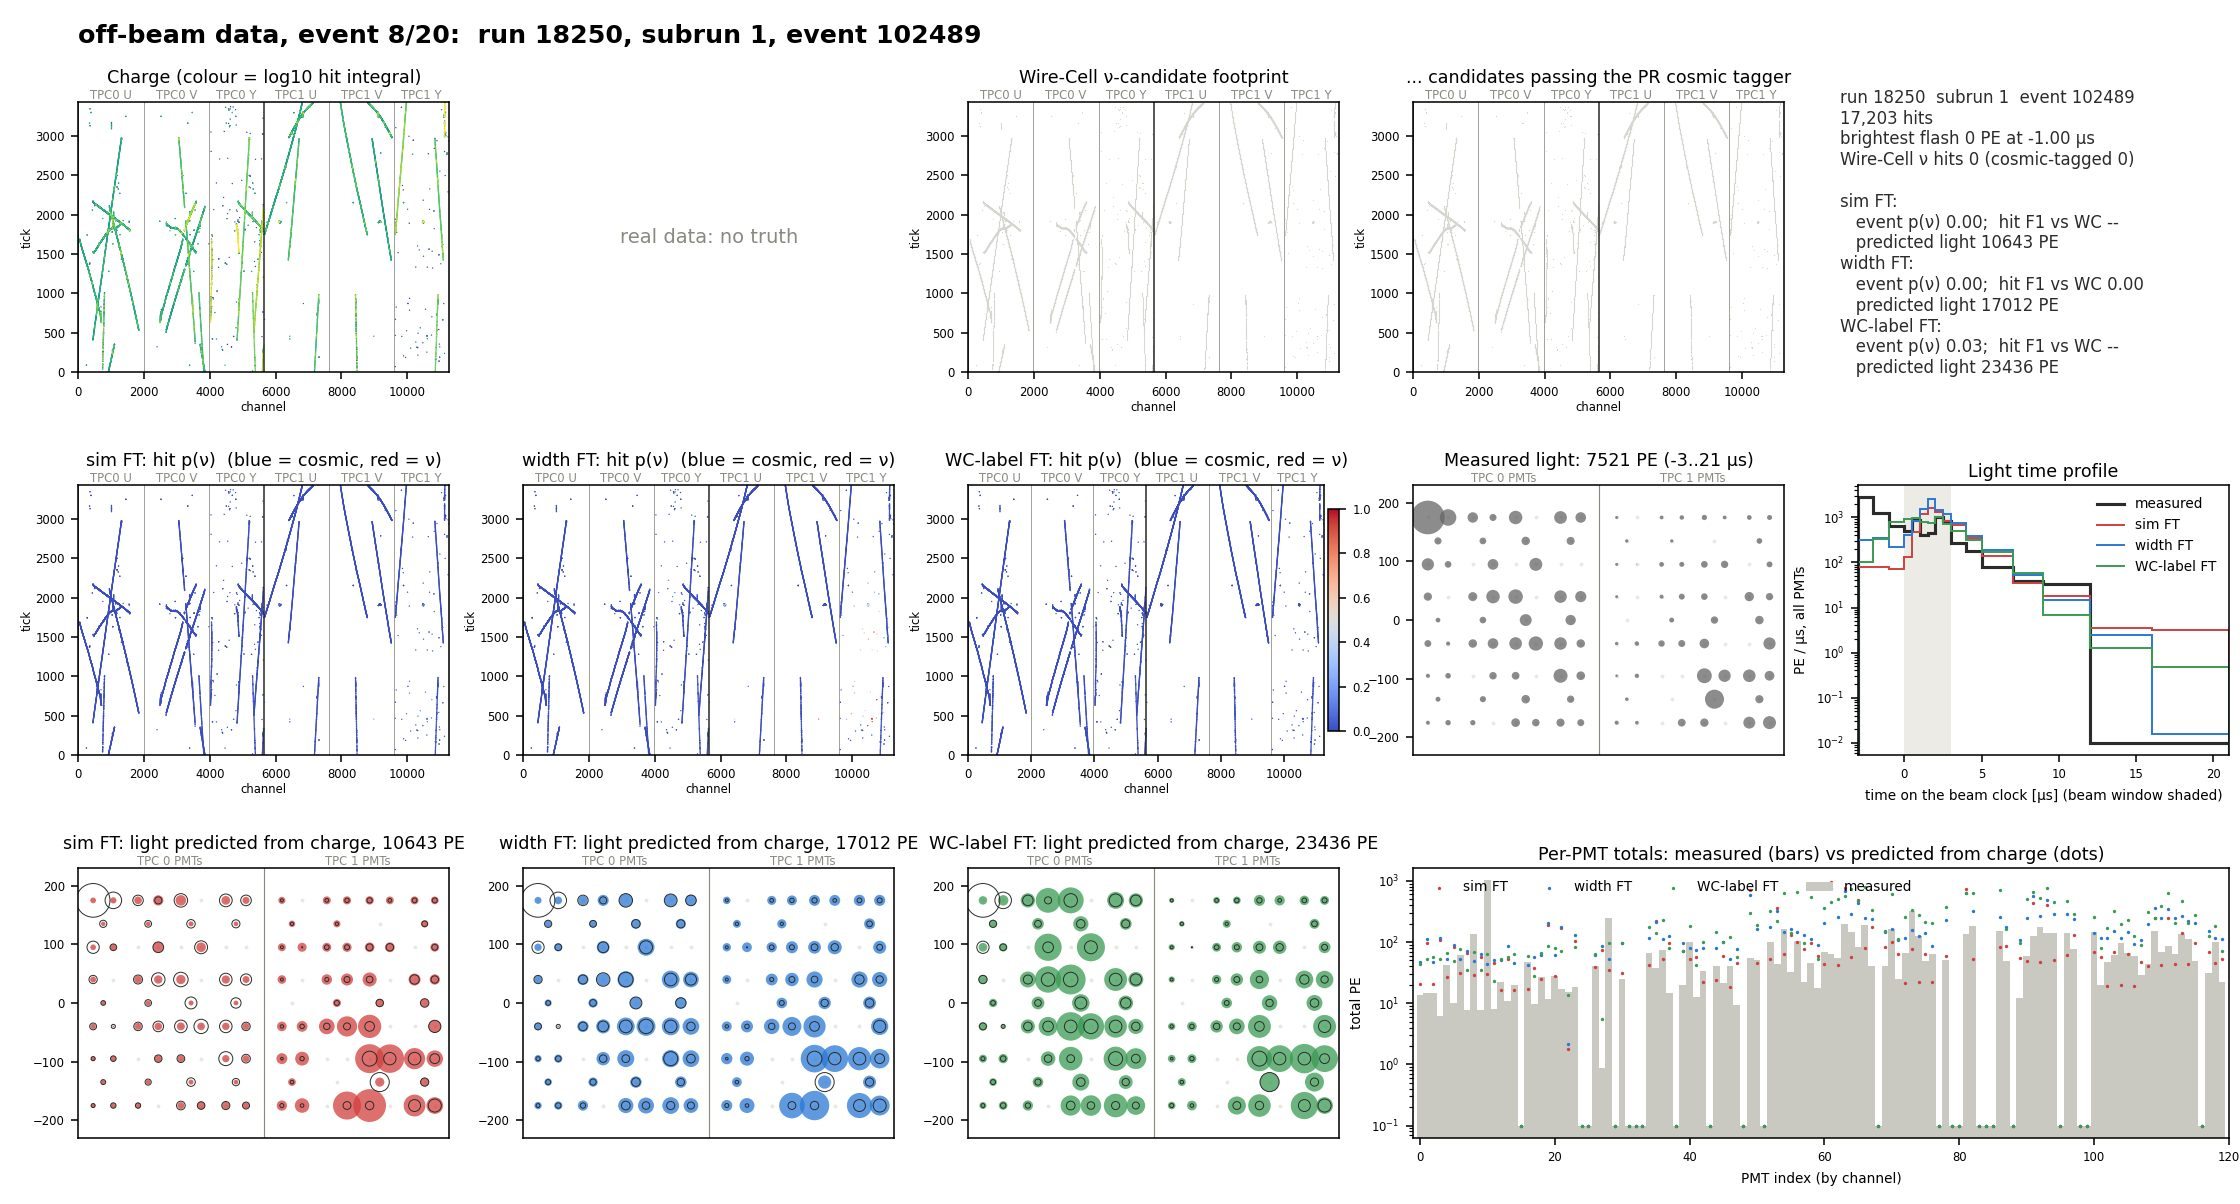
\includegraphics[width=\paperwidth,height=\paperheight,keepaspectratio]{displays/off_07.jpg}}
\end{frame}
% Off-beam data 9/20: run 18365, subrun 1, event 245600; event p(nu): sim FT 0.00, width FT 0.00, WC-label FT 0.05
\begin{frame}[plain]
  \centering\vspace*{-2pt}
  \makebox[\linewidth][c]{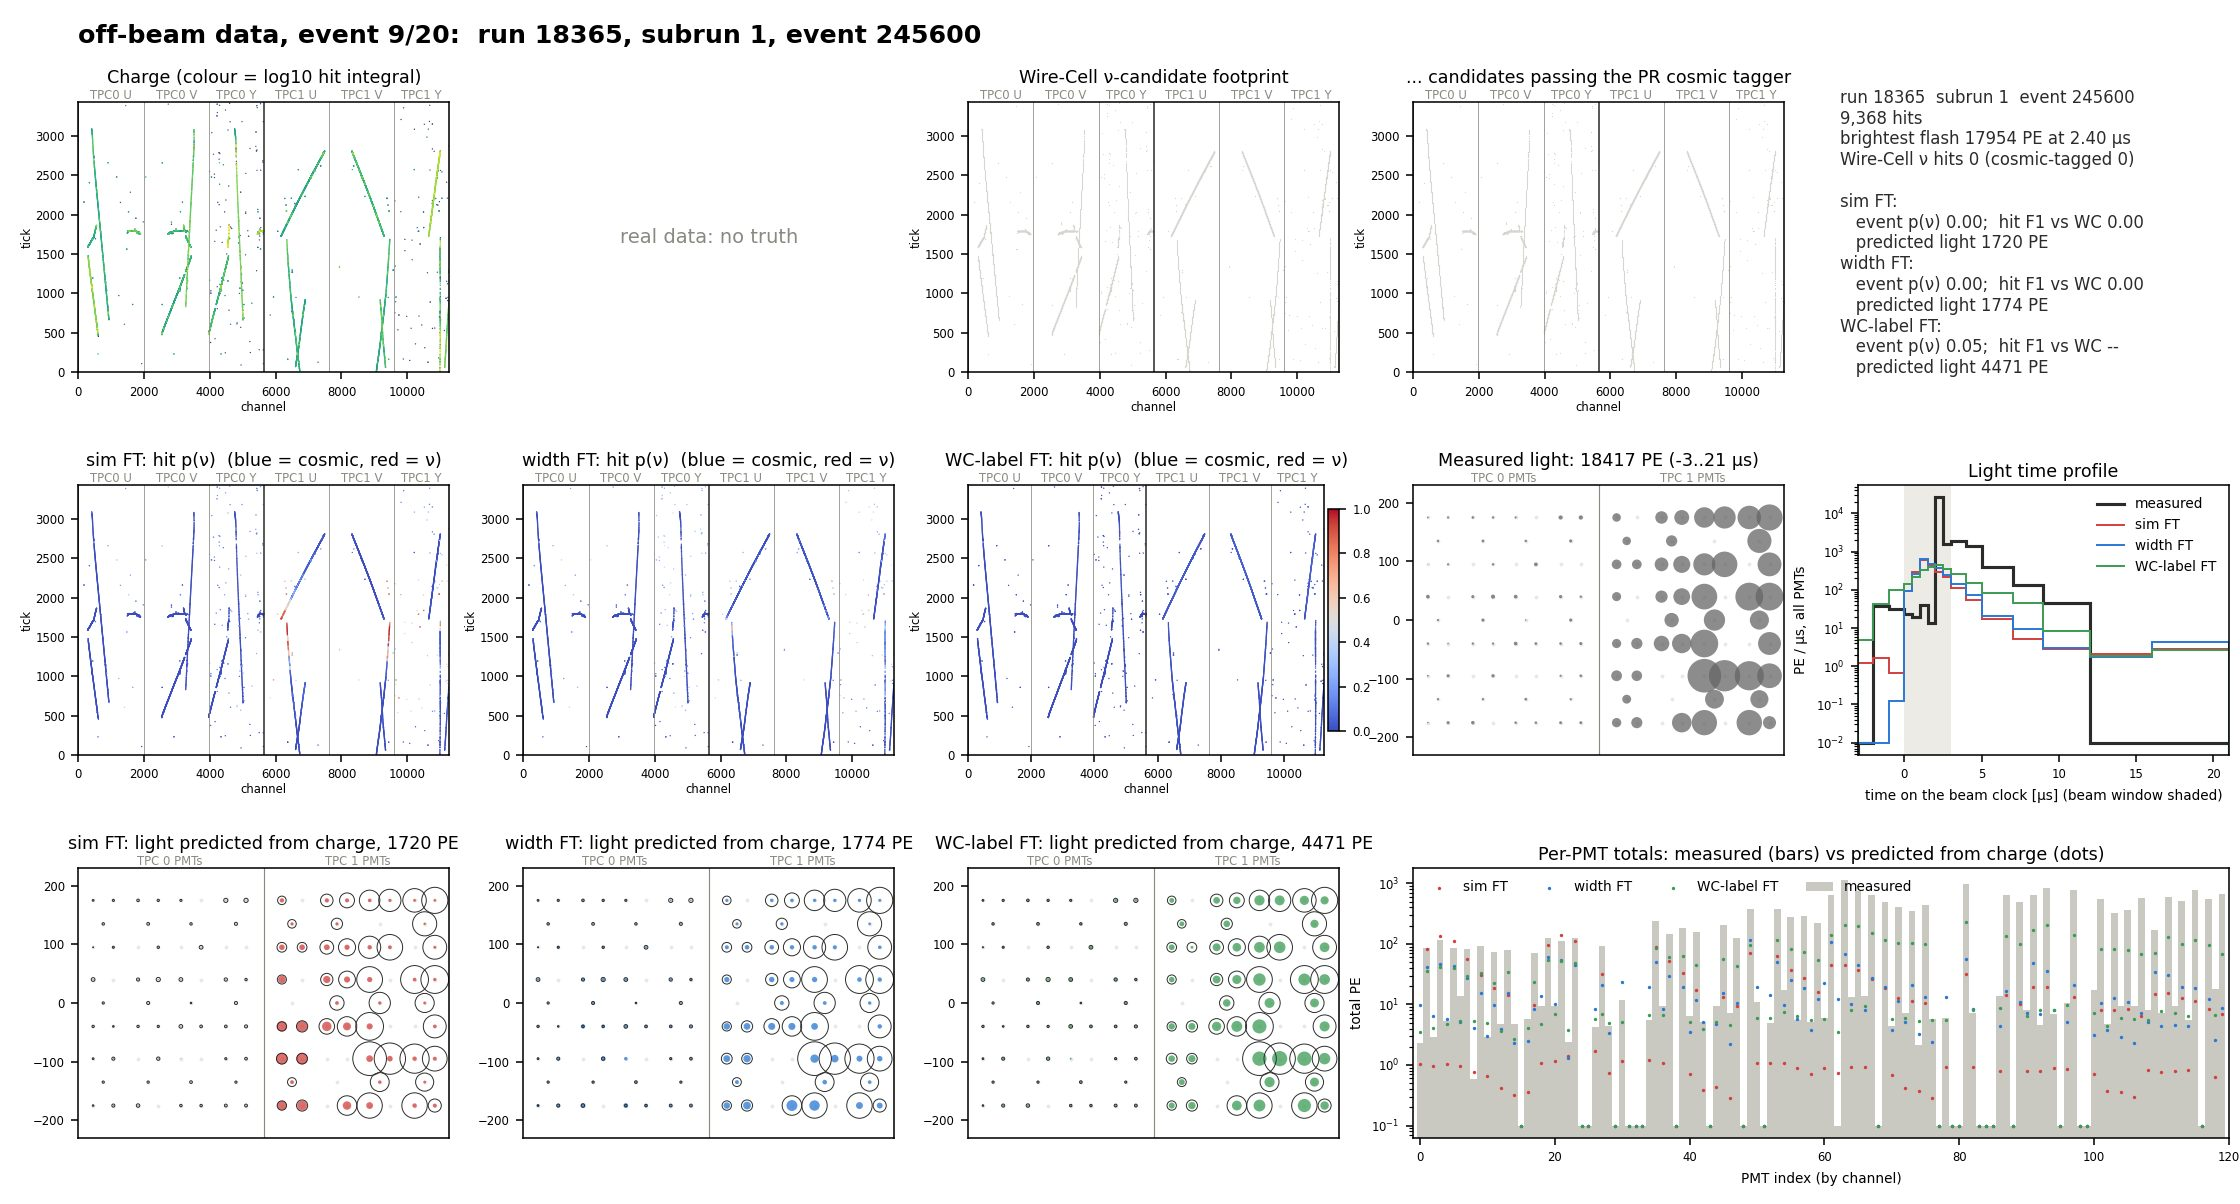
\includegraphics[width=\paperwidth,height=\paperheight,keepaspectratio]{displays/off_08.jpg}}
\end{frame}
% Off-beam data 10/20: run 18509, subrun 1, event 2583; event p(nu): sim FT 0.00, width FT 0.00, WC-label FT 0.15
\begin{frame}[plain]
  \centering\vspace*{-2pt}
  \makebox[\linewidth][c]{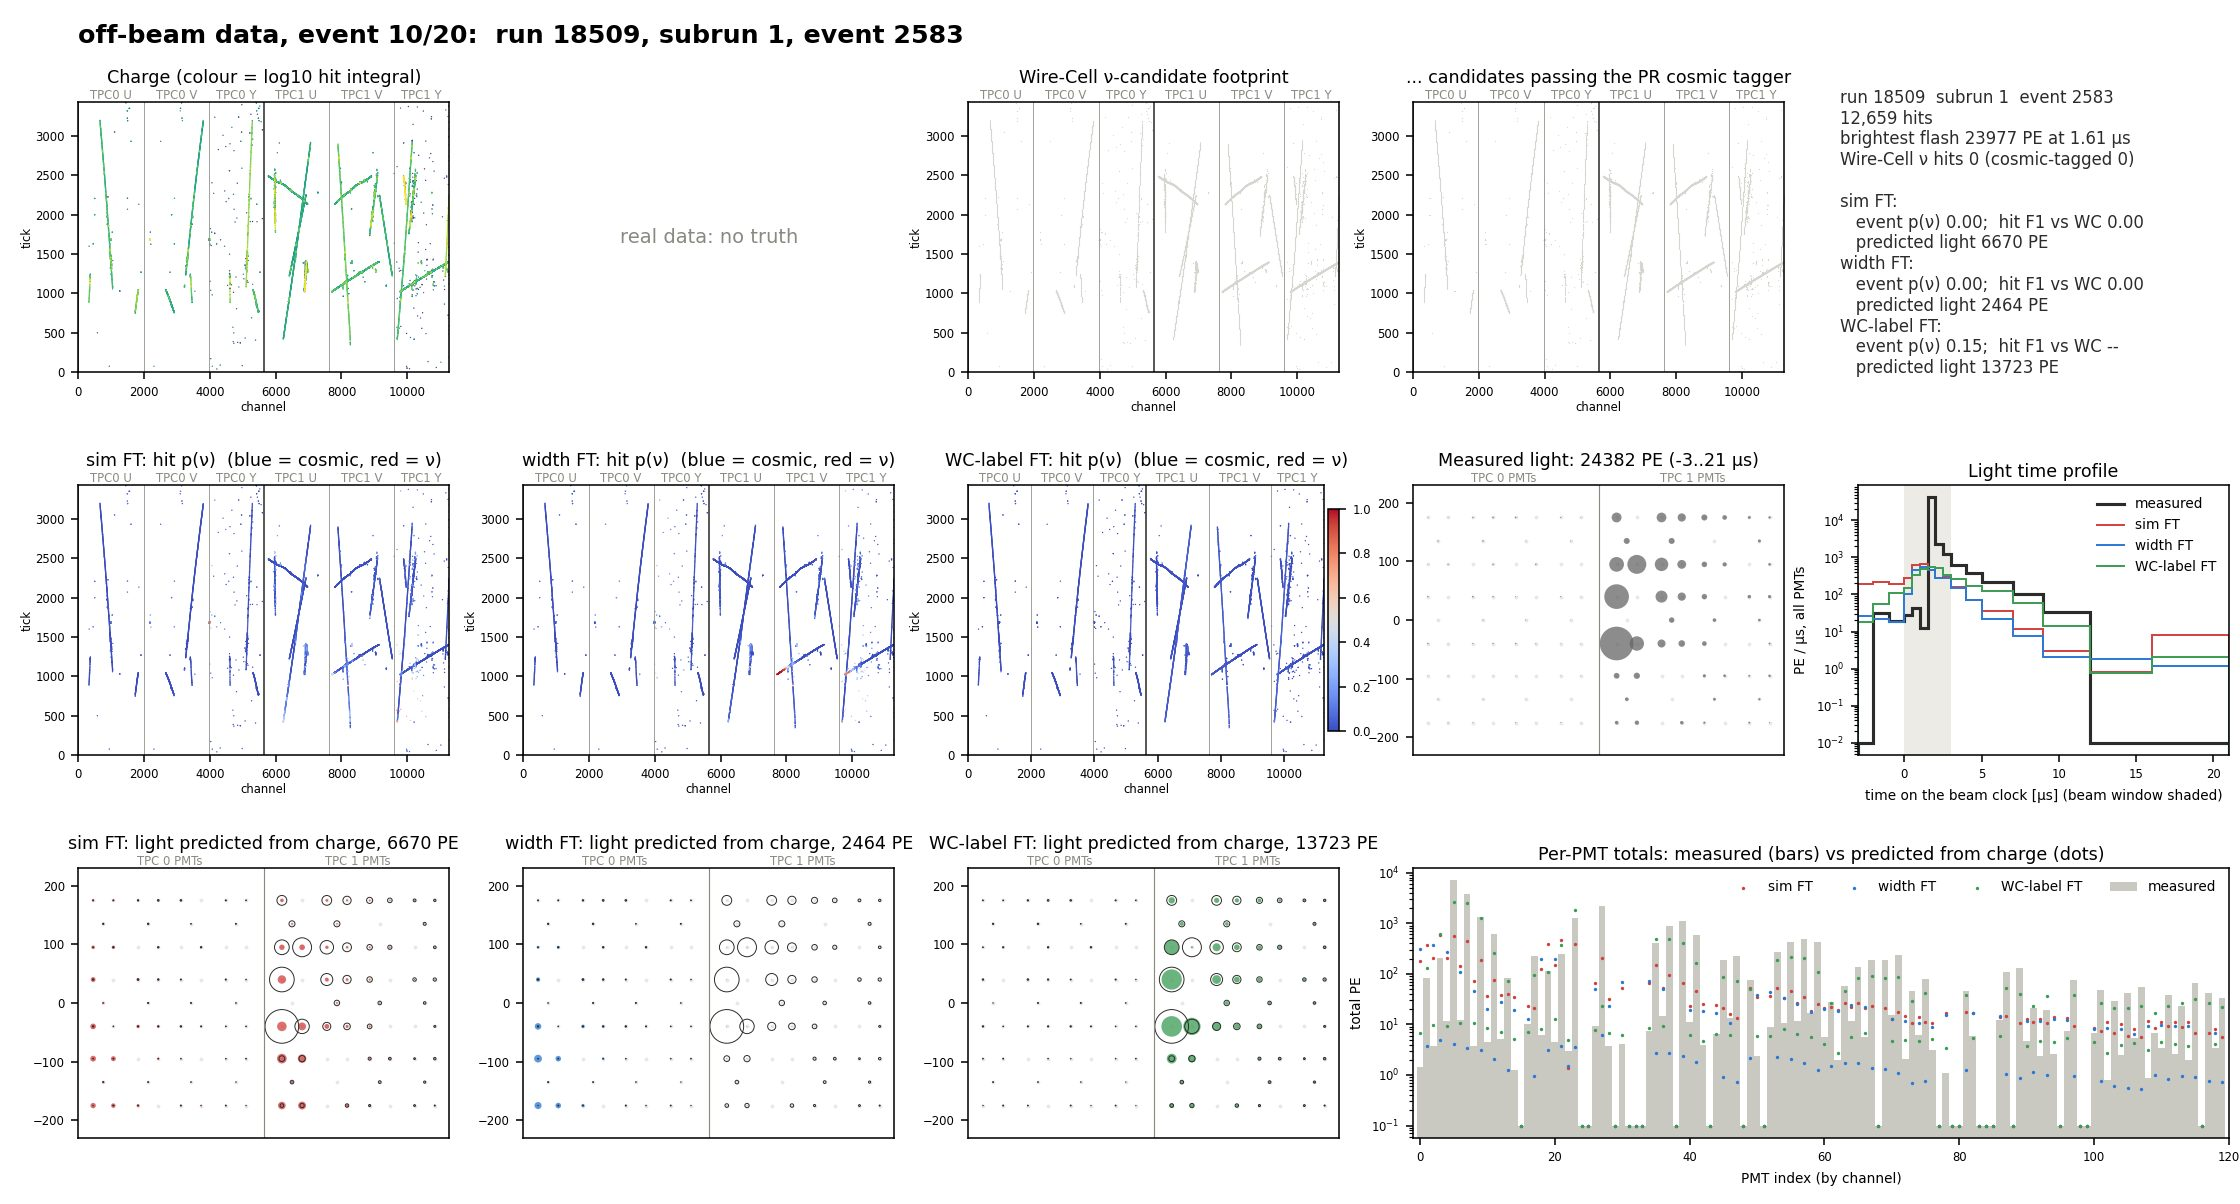
\includegraphics[width=\paperwidth,height=\paperheight,keepaspectratio]{displays/off_09.jpg}}
\end{frame}
% Off-beam data 11/20: run 18259, subrun 1, event 133561; event p(nu): sim FT 0.00, width FT 0.00, WC-label FT 0.00
\begin{frame}[plain]
  \centering\vspace*{-2pt}
  \makebox[\linewidth][c]{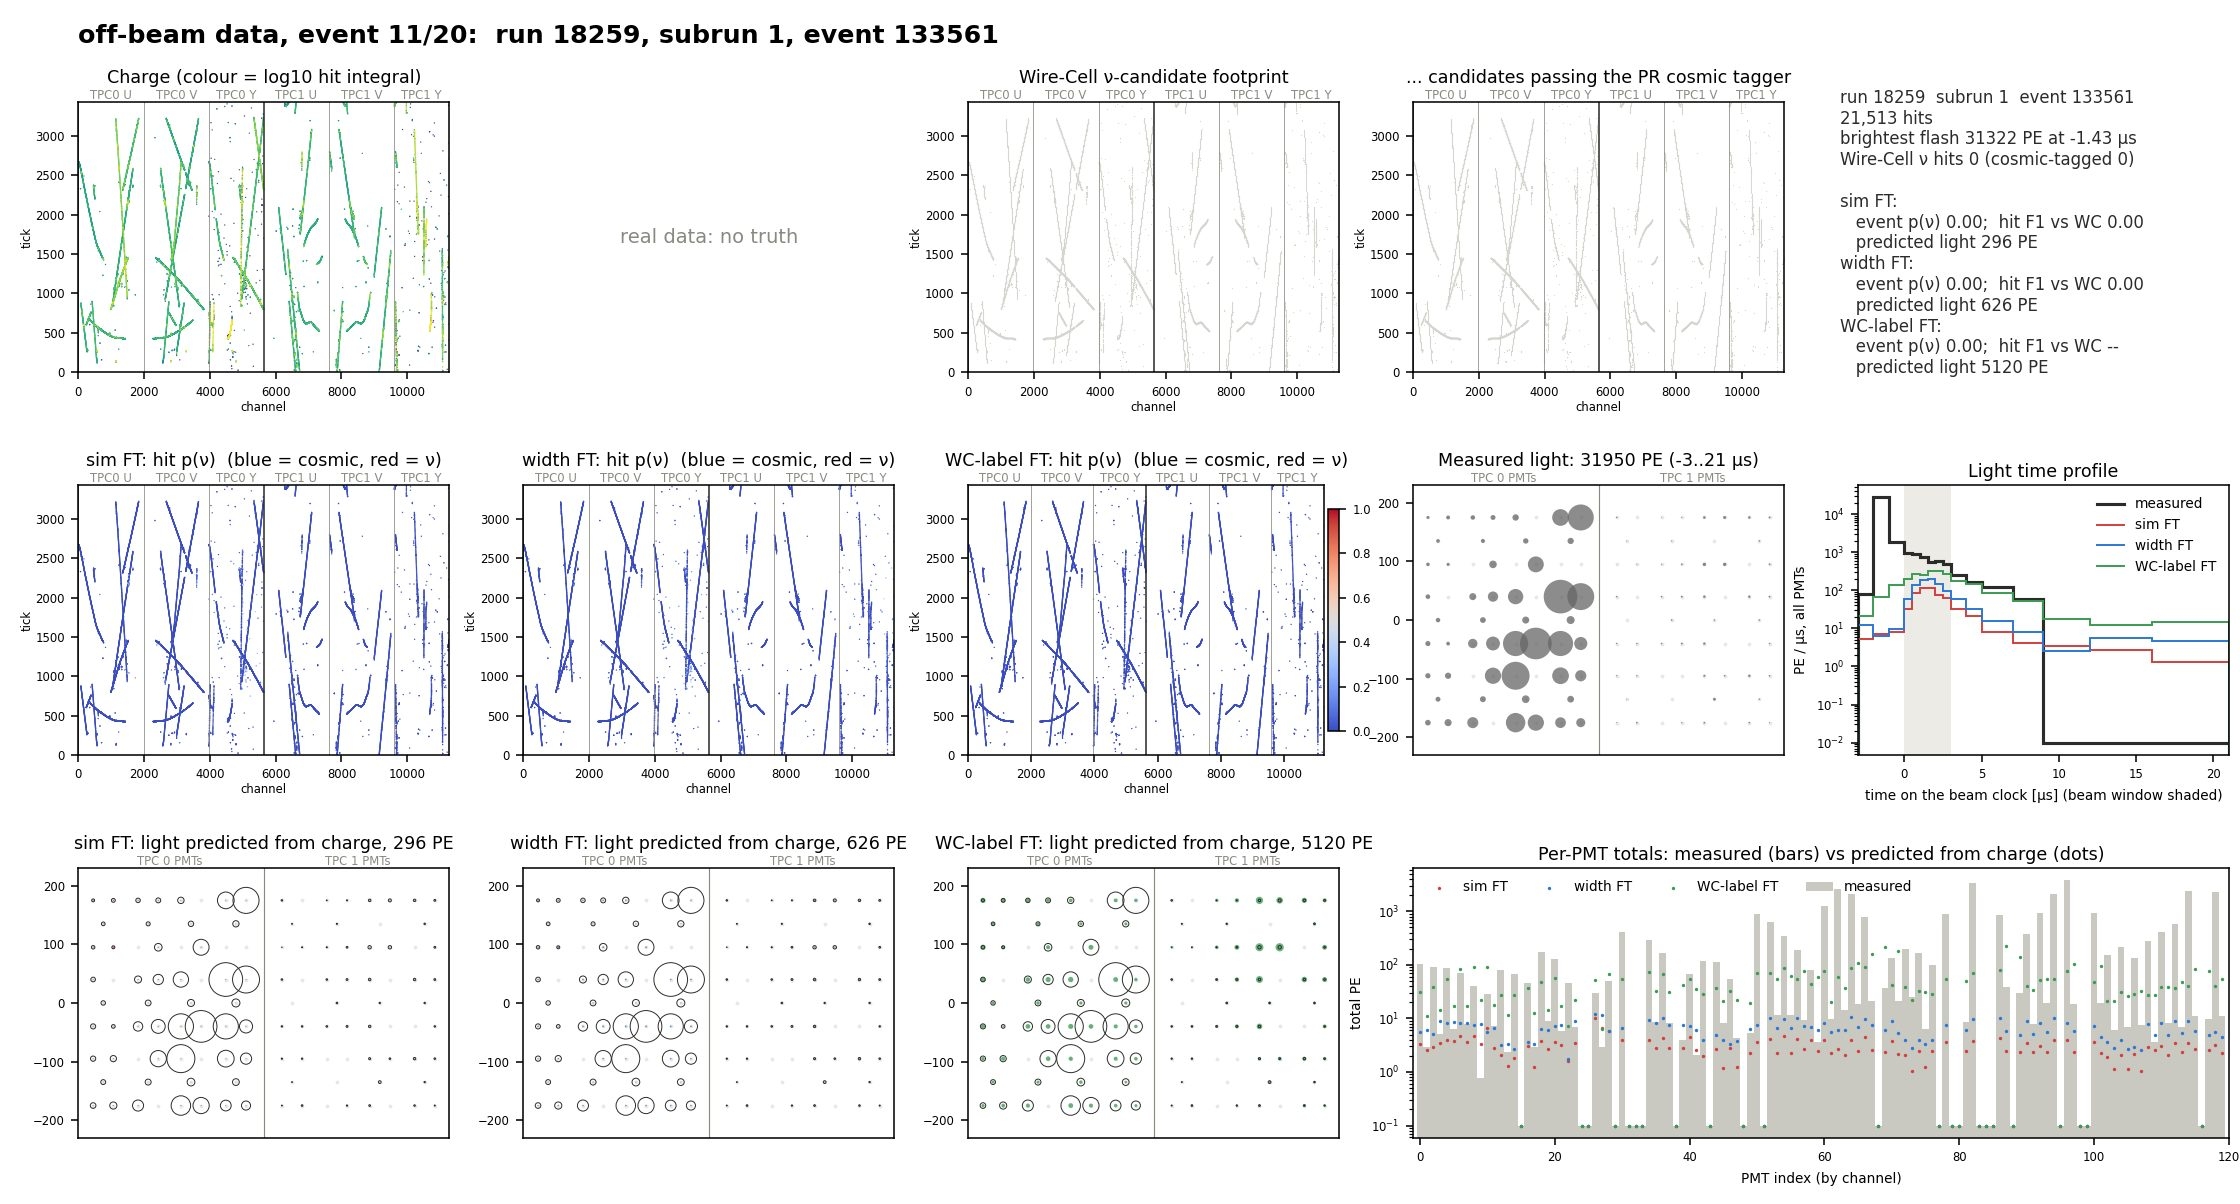
\includegraphics[width=\paperwidth,height=\paperheight,keepaspectratio]{displays/off_10.jpg}}
\end{frame}
% Off-beam data 12/20: run 18334, subrun 1, event 105361; event p(nu): sim FT 0.00, width FT 0.00, WC-label FT 0.09
\begin{frame}[plain]
  \centering\vspace*{-2pt}
  \makebox[\linewidth][c]{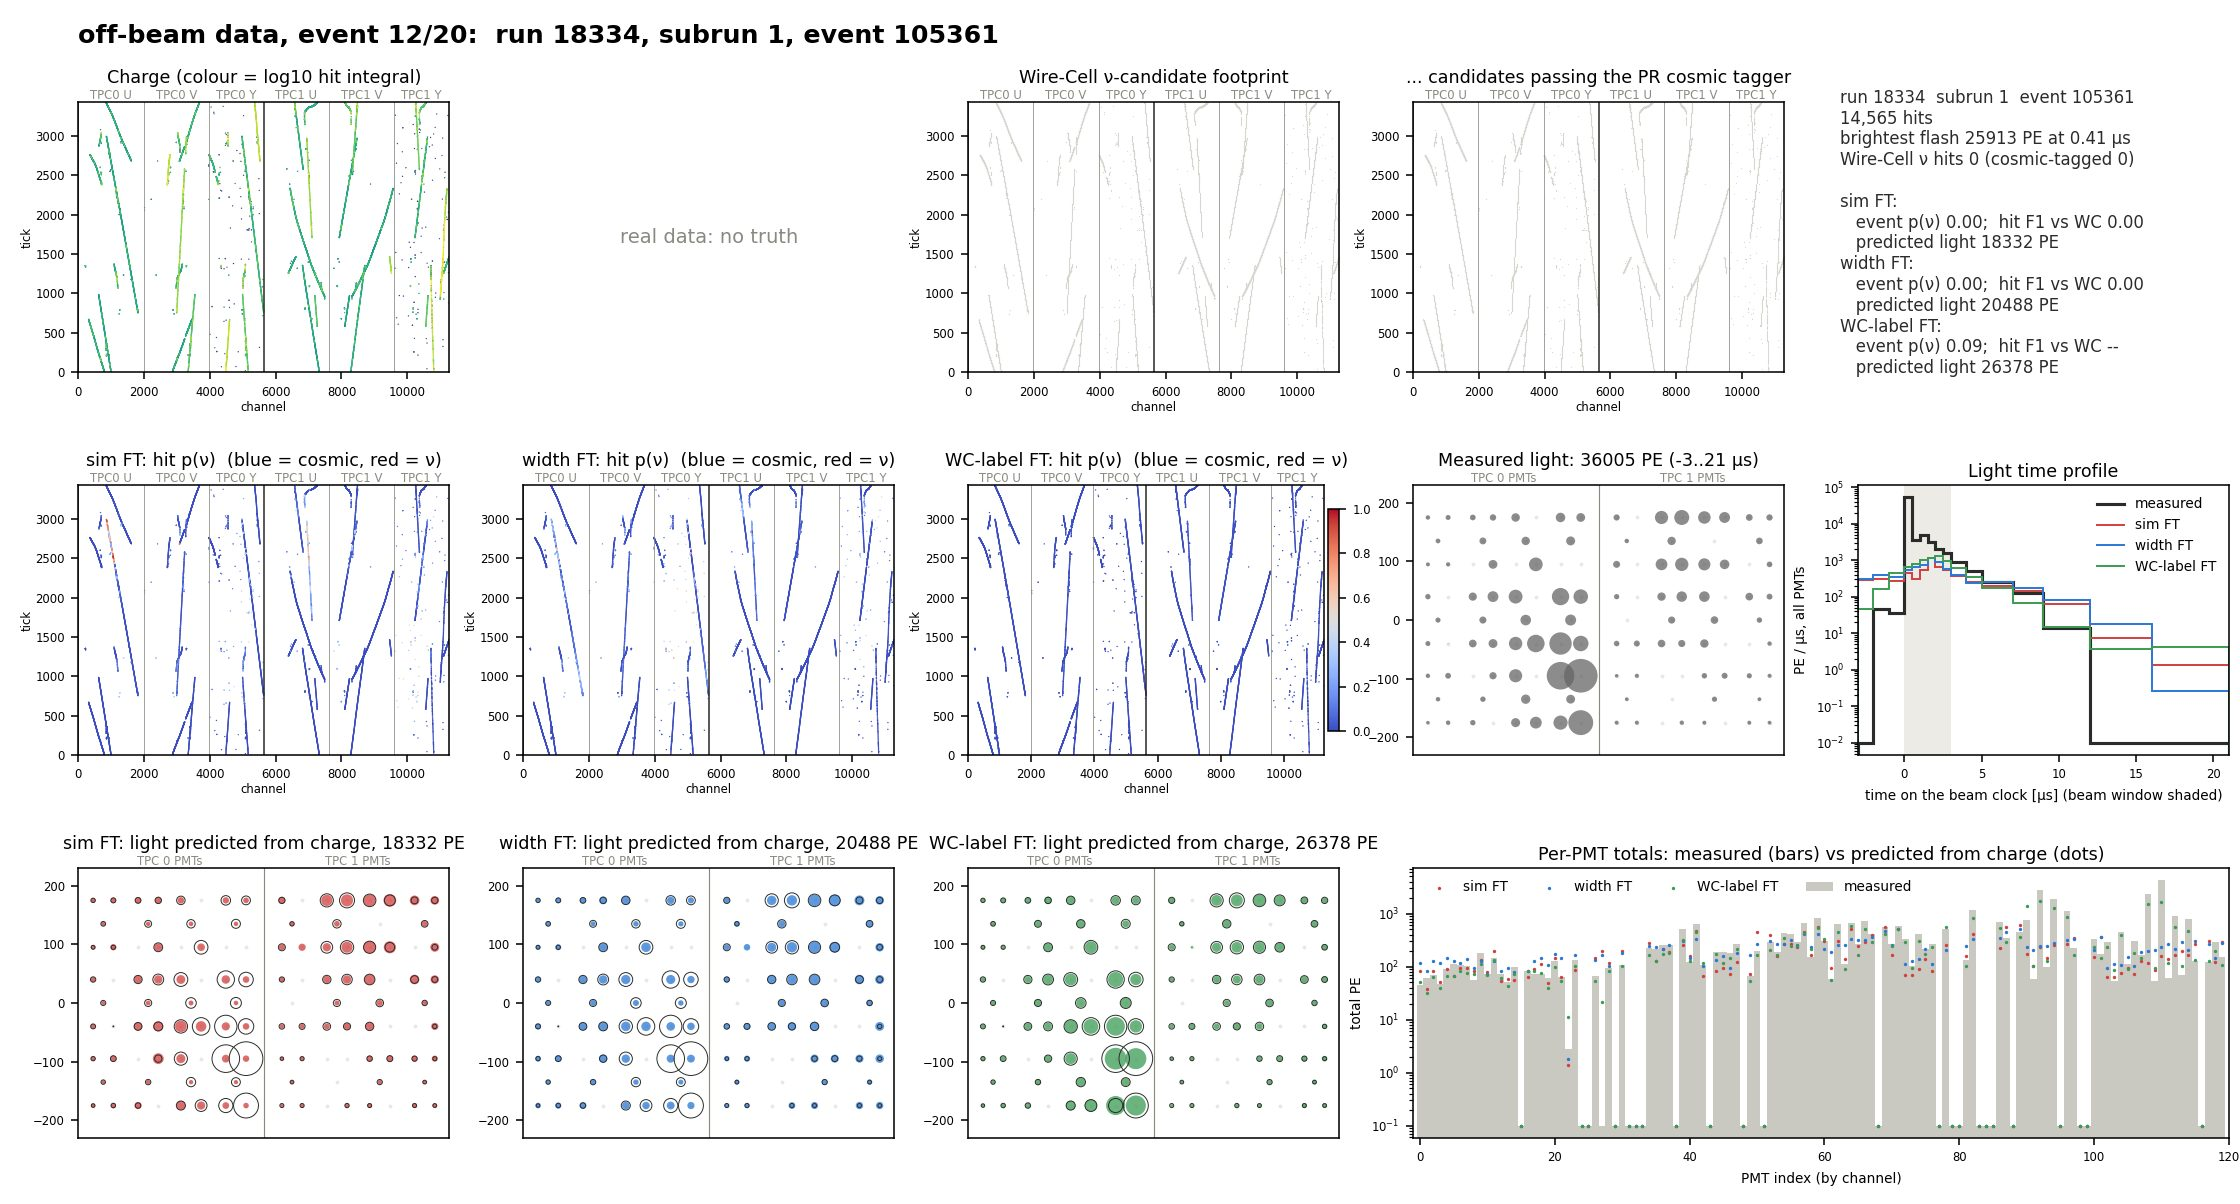
\includegraphics[width=\paperwidth,height=\paperheight,keepaspectratio]{displays/off_11.jpg}}
\end{frame}
% Off-beam data 13/20: run 18326, subrun 1, event 145516; event p(nu): sim FT 0.00, width FT 0.00, WC-label FT 0.04
\begin{frame}[plain]
  \centering\vspace*{-2pt}
  \makebox[\linewidth][c]{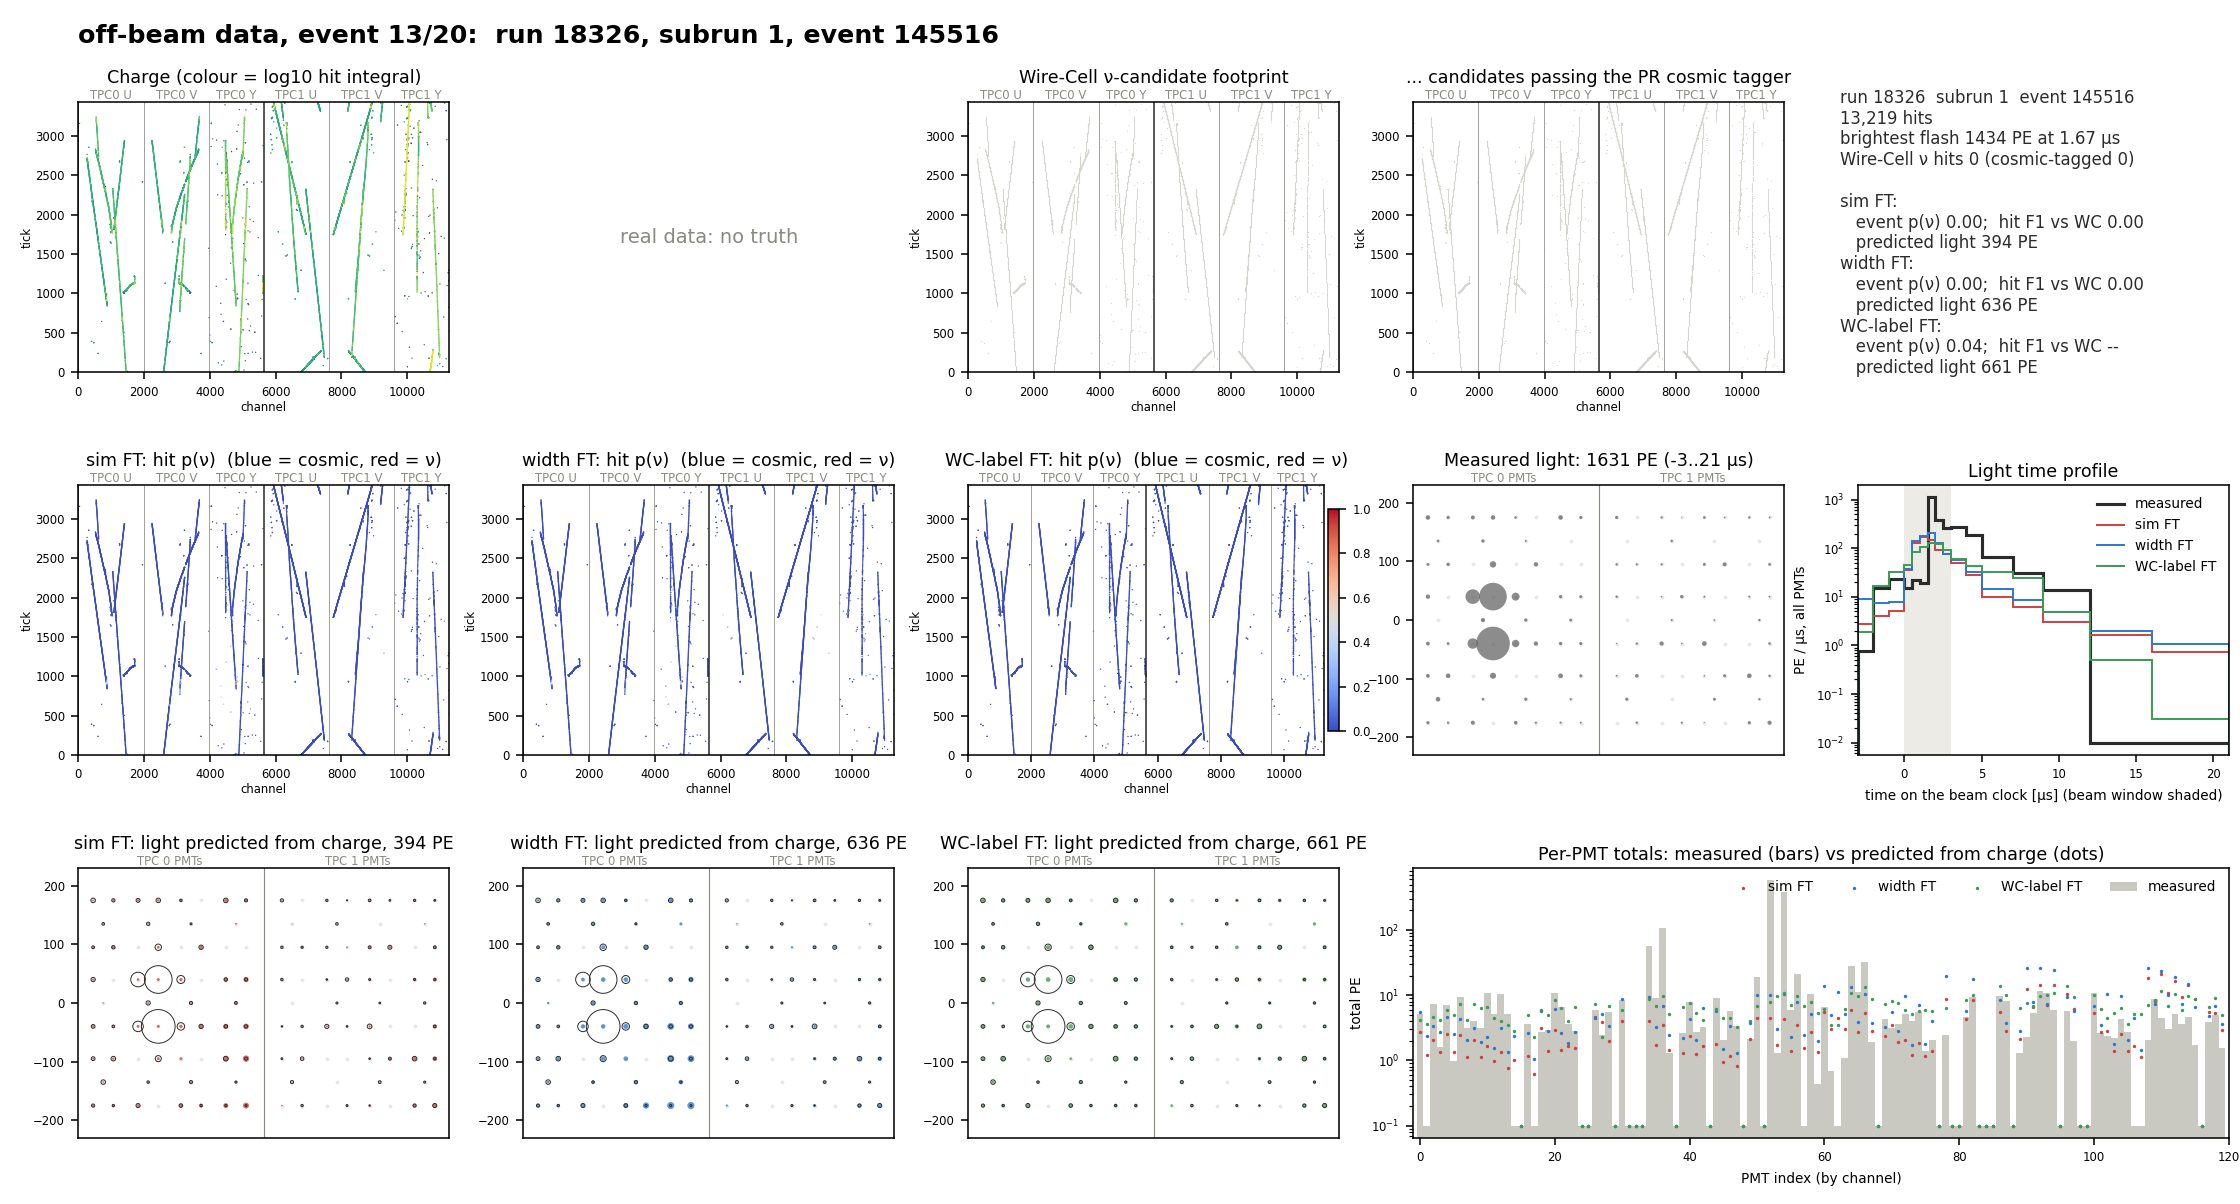
\includegraphics[width=\paperwidth,height=\paperheight,keepaspectratio]{displays/off_12.jpg}}
\end{frame}
% Off-beam data 14/20: run 18444, subrun 1, event 240124; event p(nu): sim FT 0.00, width FT 0.00, WC-label FT 0.16
\begin{frame}[plain]
  \centering\vspace*{-2pt}
  \makebox[\linewidth][c]{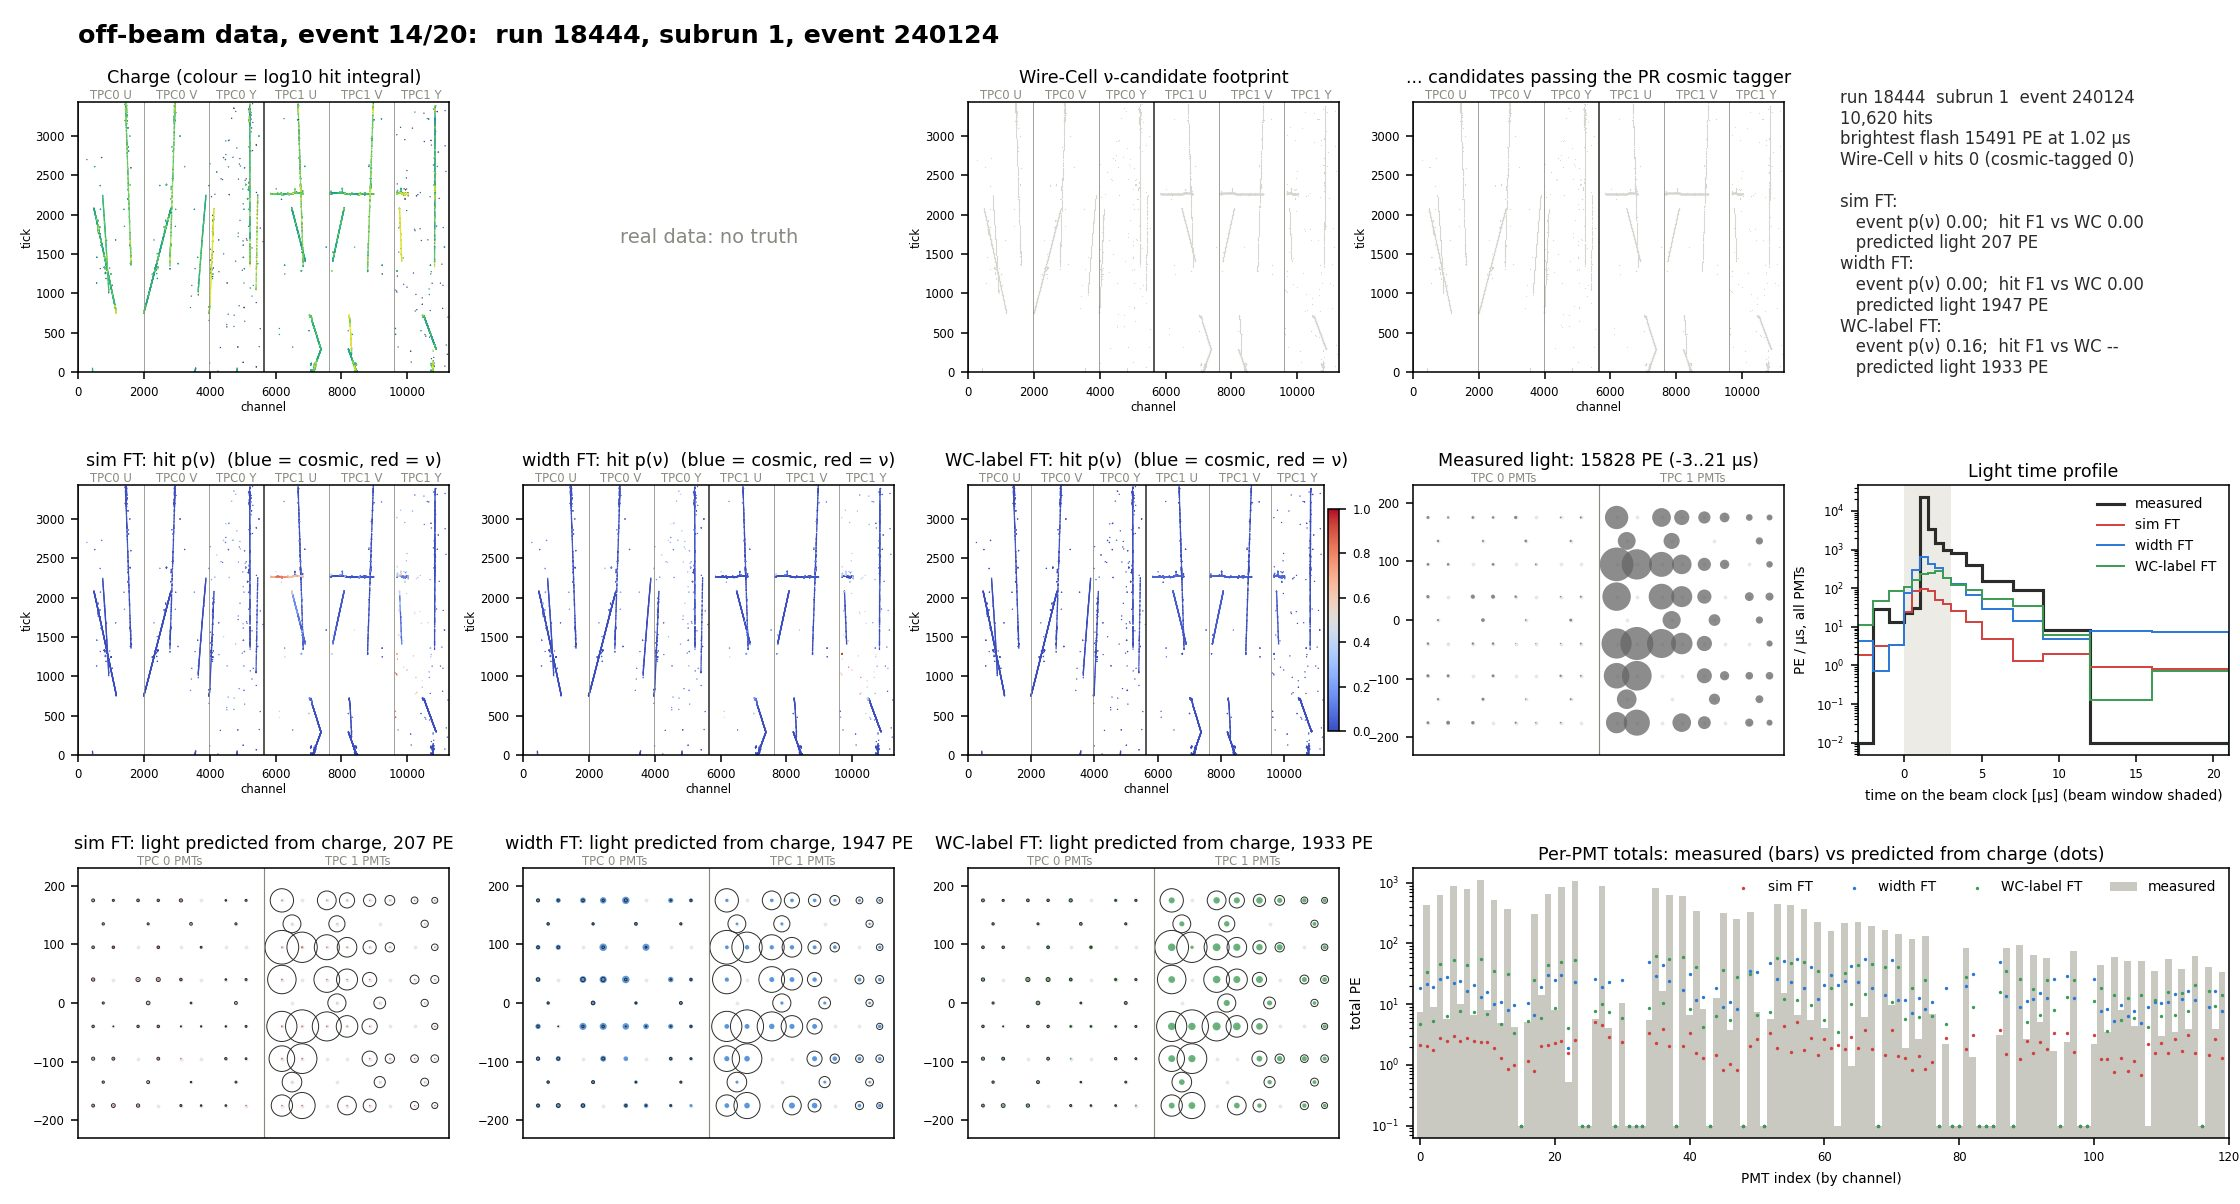
\includegraphics[width=\paperwidth,height=\paperheight,keepaspectratio]{displays/off_13.jpg}}
\end{frame}
% Off-beam data 15/20: run 18453, subrun 1, event 94673; event p(nu): sim FT 0.35, width FT 1.00, WC-label FT 0.15
\begin{frame}[plain]
  \centering\vspace*{-2pt}
  \makebox[\linewidth][c]{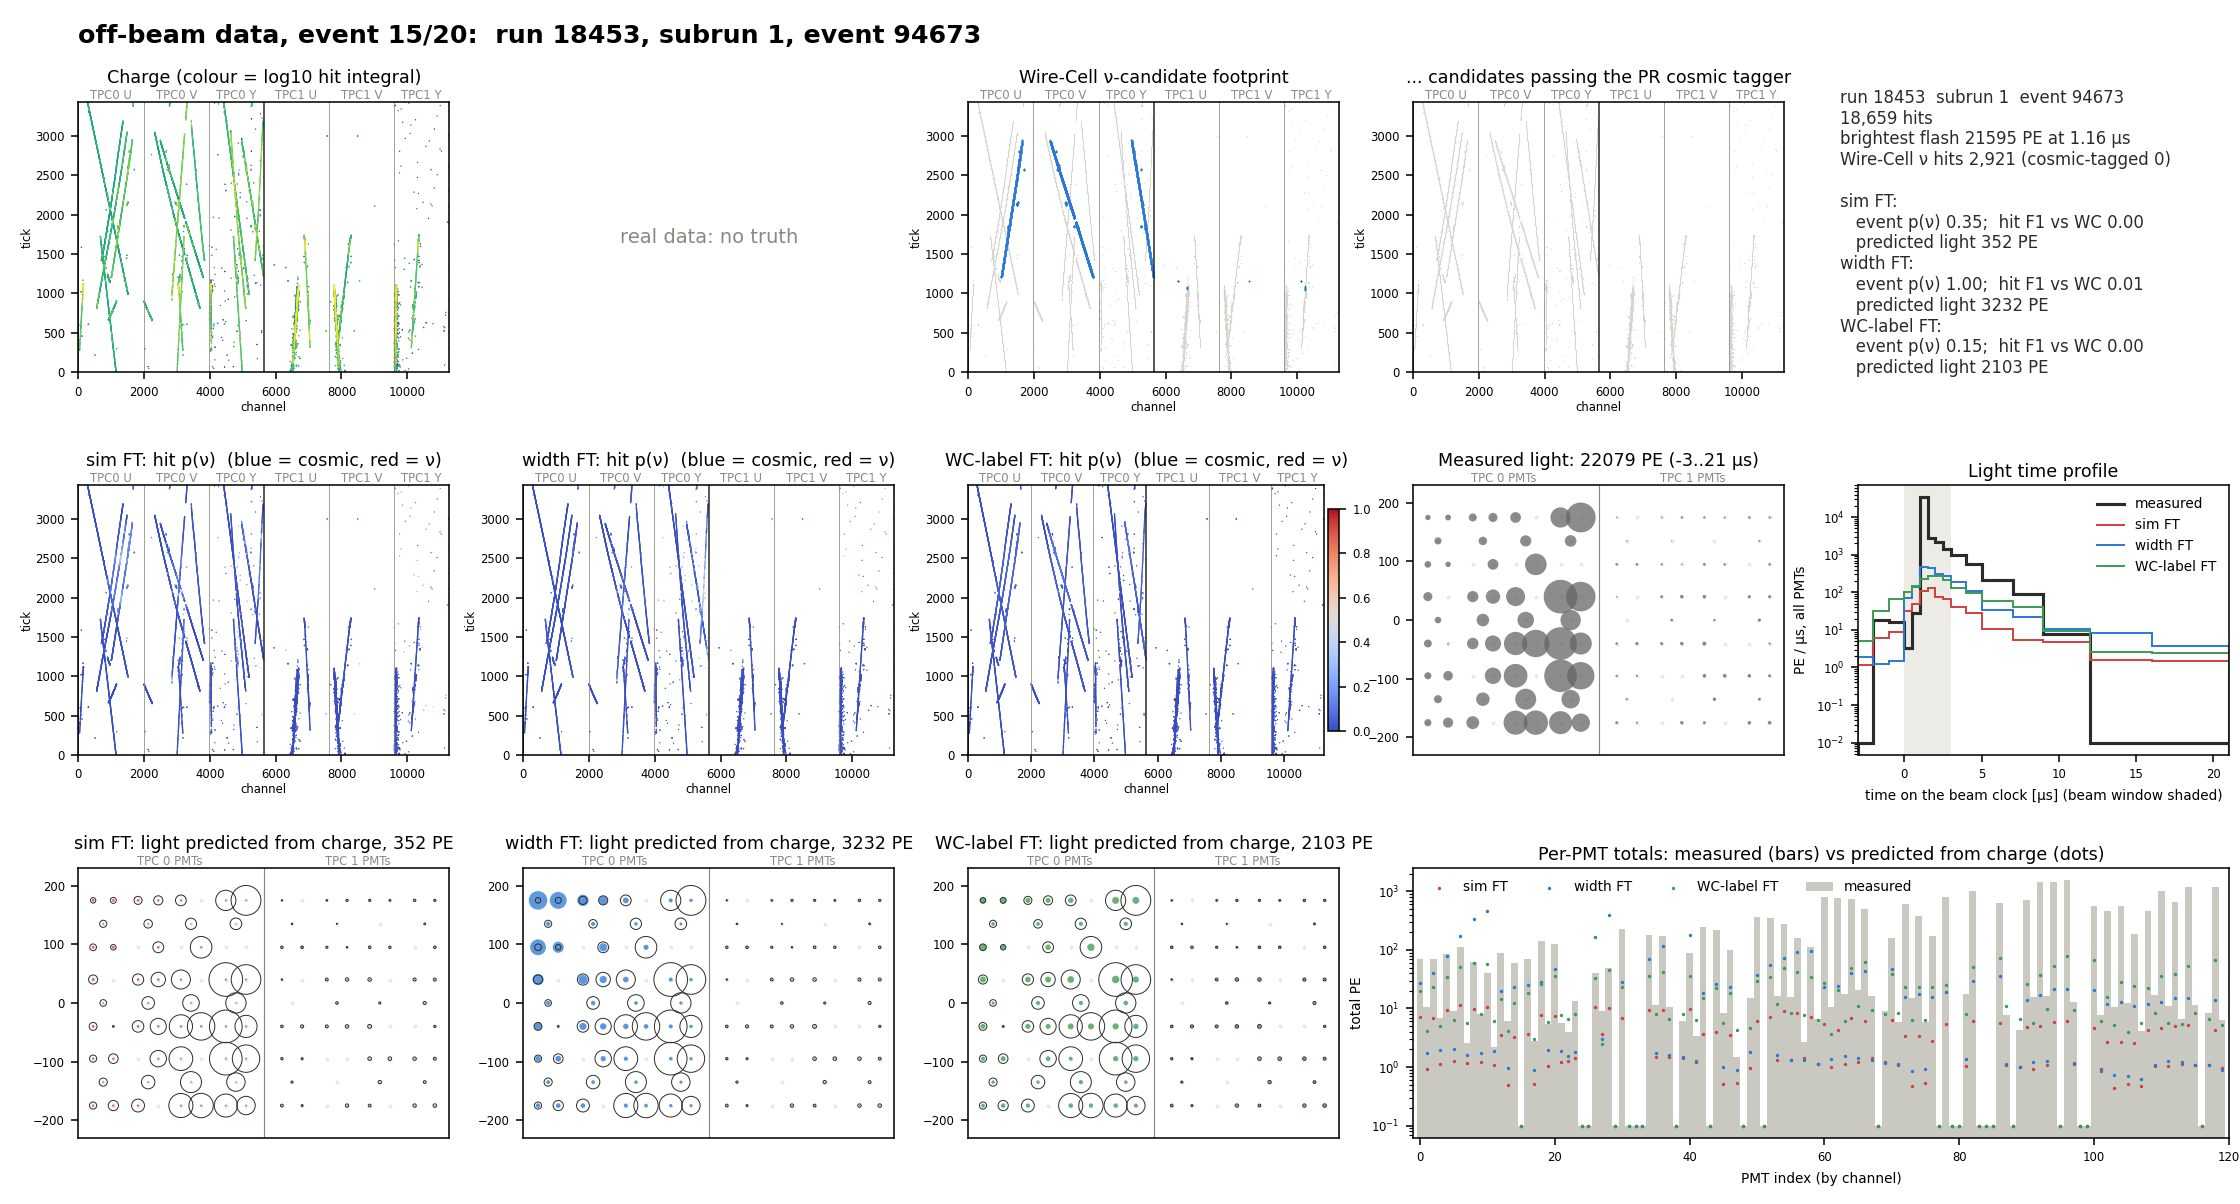
\includegraphics[width=\paperwidth,height=\paperheight,keepaspectratio]{displays/off_14.jpg}}
\end{frame}
% Off-beam data 16/20: run 18485, subrun 1, event 226962; event p(nu): sim FT 0.00, width FT 0.00, WC-label FT 0.01
\begin{frame}[plain]
  \centering\vspace*{-2pt}
  \makebox[\linewidth][c]{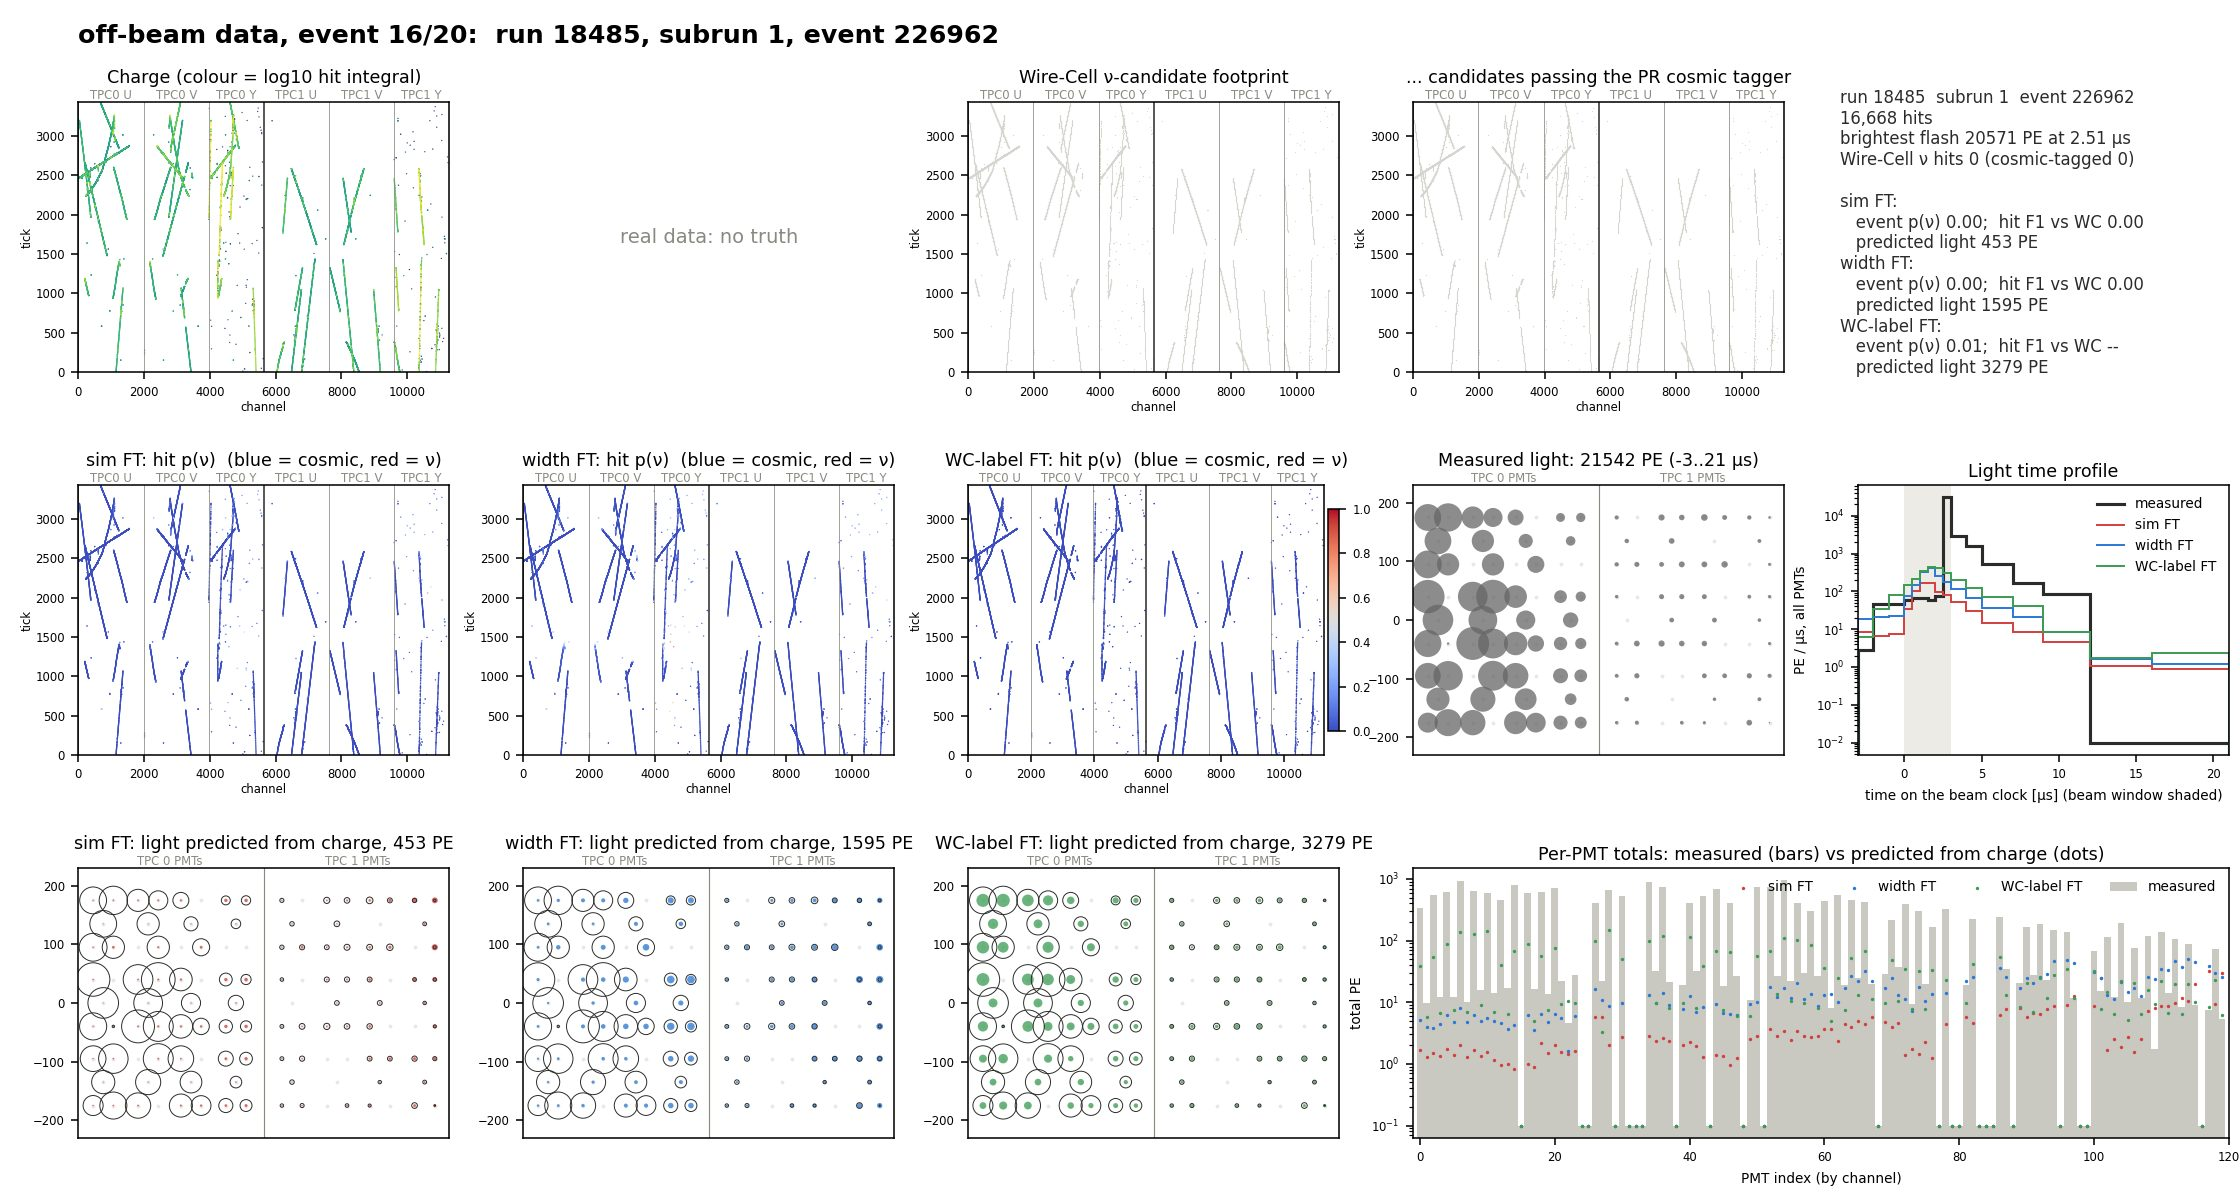
\includegraphics[width=\paperwidth,height=\paperheight,keepaspectratio]{displays/off_15.jpg}}
\end{frame}
% Off-beam data 17/20: run 18576, subrun 1, event 123870; event p(nu): sim FT 1.00, width FT 0.00, WC-label FT 0.29
\begin{frame}[plain]
  \centering\vspace*{-2pt}
  \makebox[\linewidth][c]{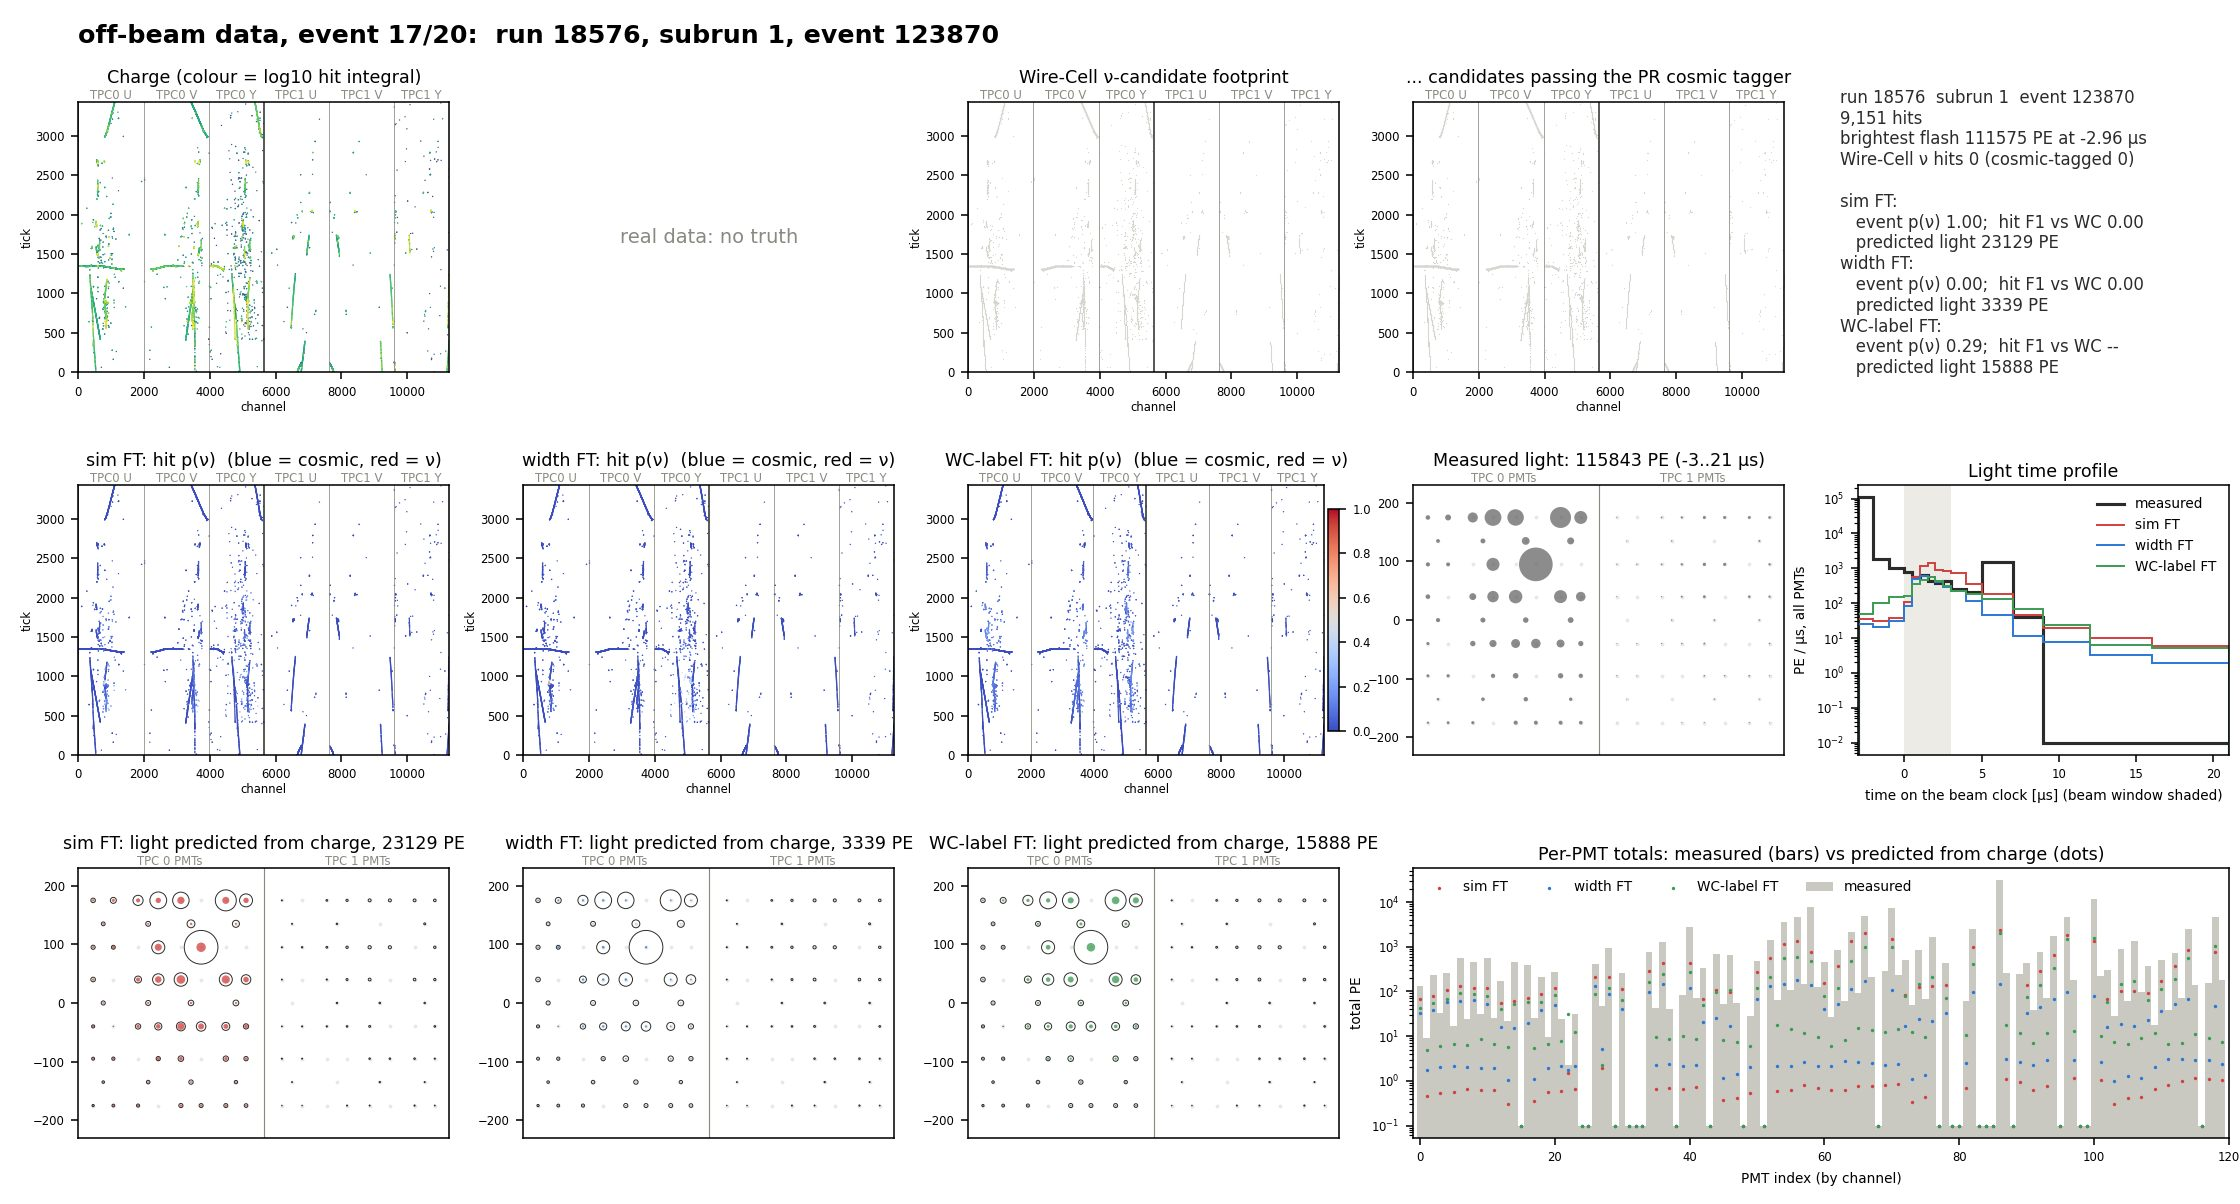
\includegraphics[width=\paperwidth,height=\paperheight,keepaspectratio]{displays/off_16.jpg}}
\end{frame}
% Off-beam data 18/20: run 18503, subrun 1, event 984786; event p(nu): sim FT 0.99, width FT 1.00, WC-label FT 0.08
\begin{frame}[plain]
  \centering\vspace*{-2pt}
  \makebox[\linewidth][c]{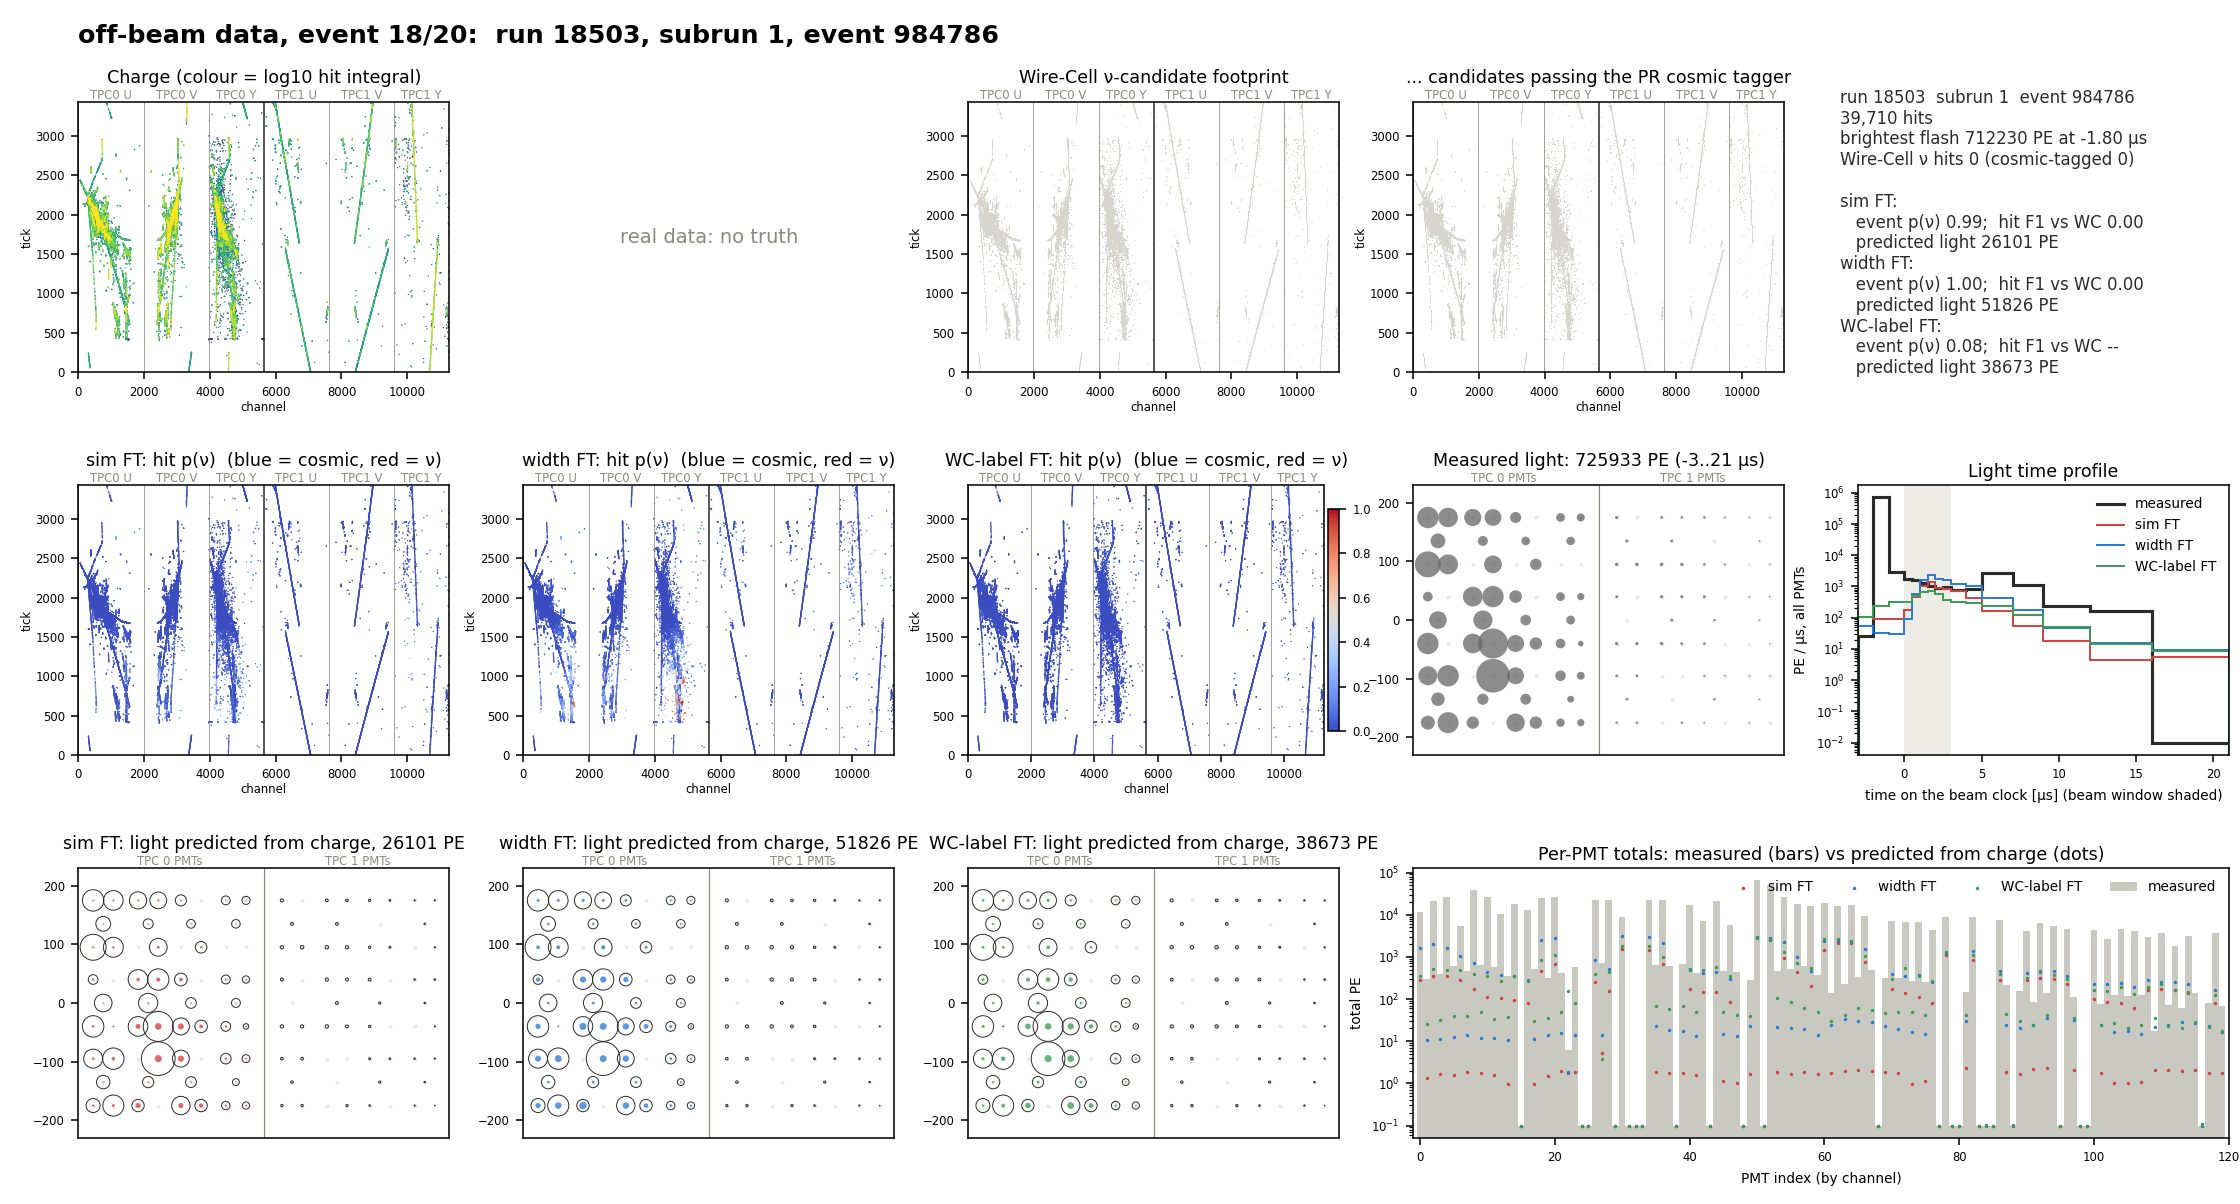
\includegraphics[width=\paperwidth,height=\paperheight,keepaspectratio]{displays/off_17.jpg}}
\end{frame}
% Off-beam data 19/20: run 18504, subrun 1, event 707279; event p(nu): sim FT 0.00, width FT 0.00, WC-label FT 0.02
\begin{frame}[plain]
  \centering\vspace*{-2pt}
  \makebox[\linewidth][c]{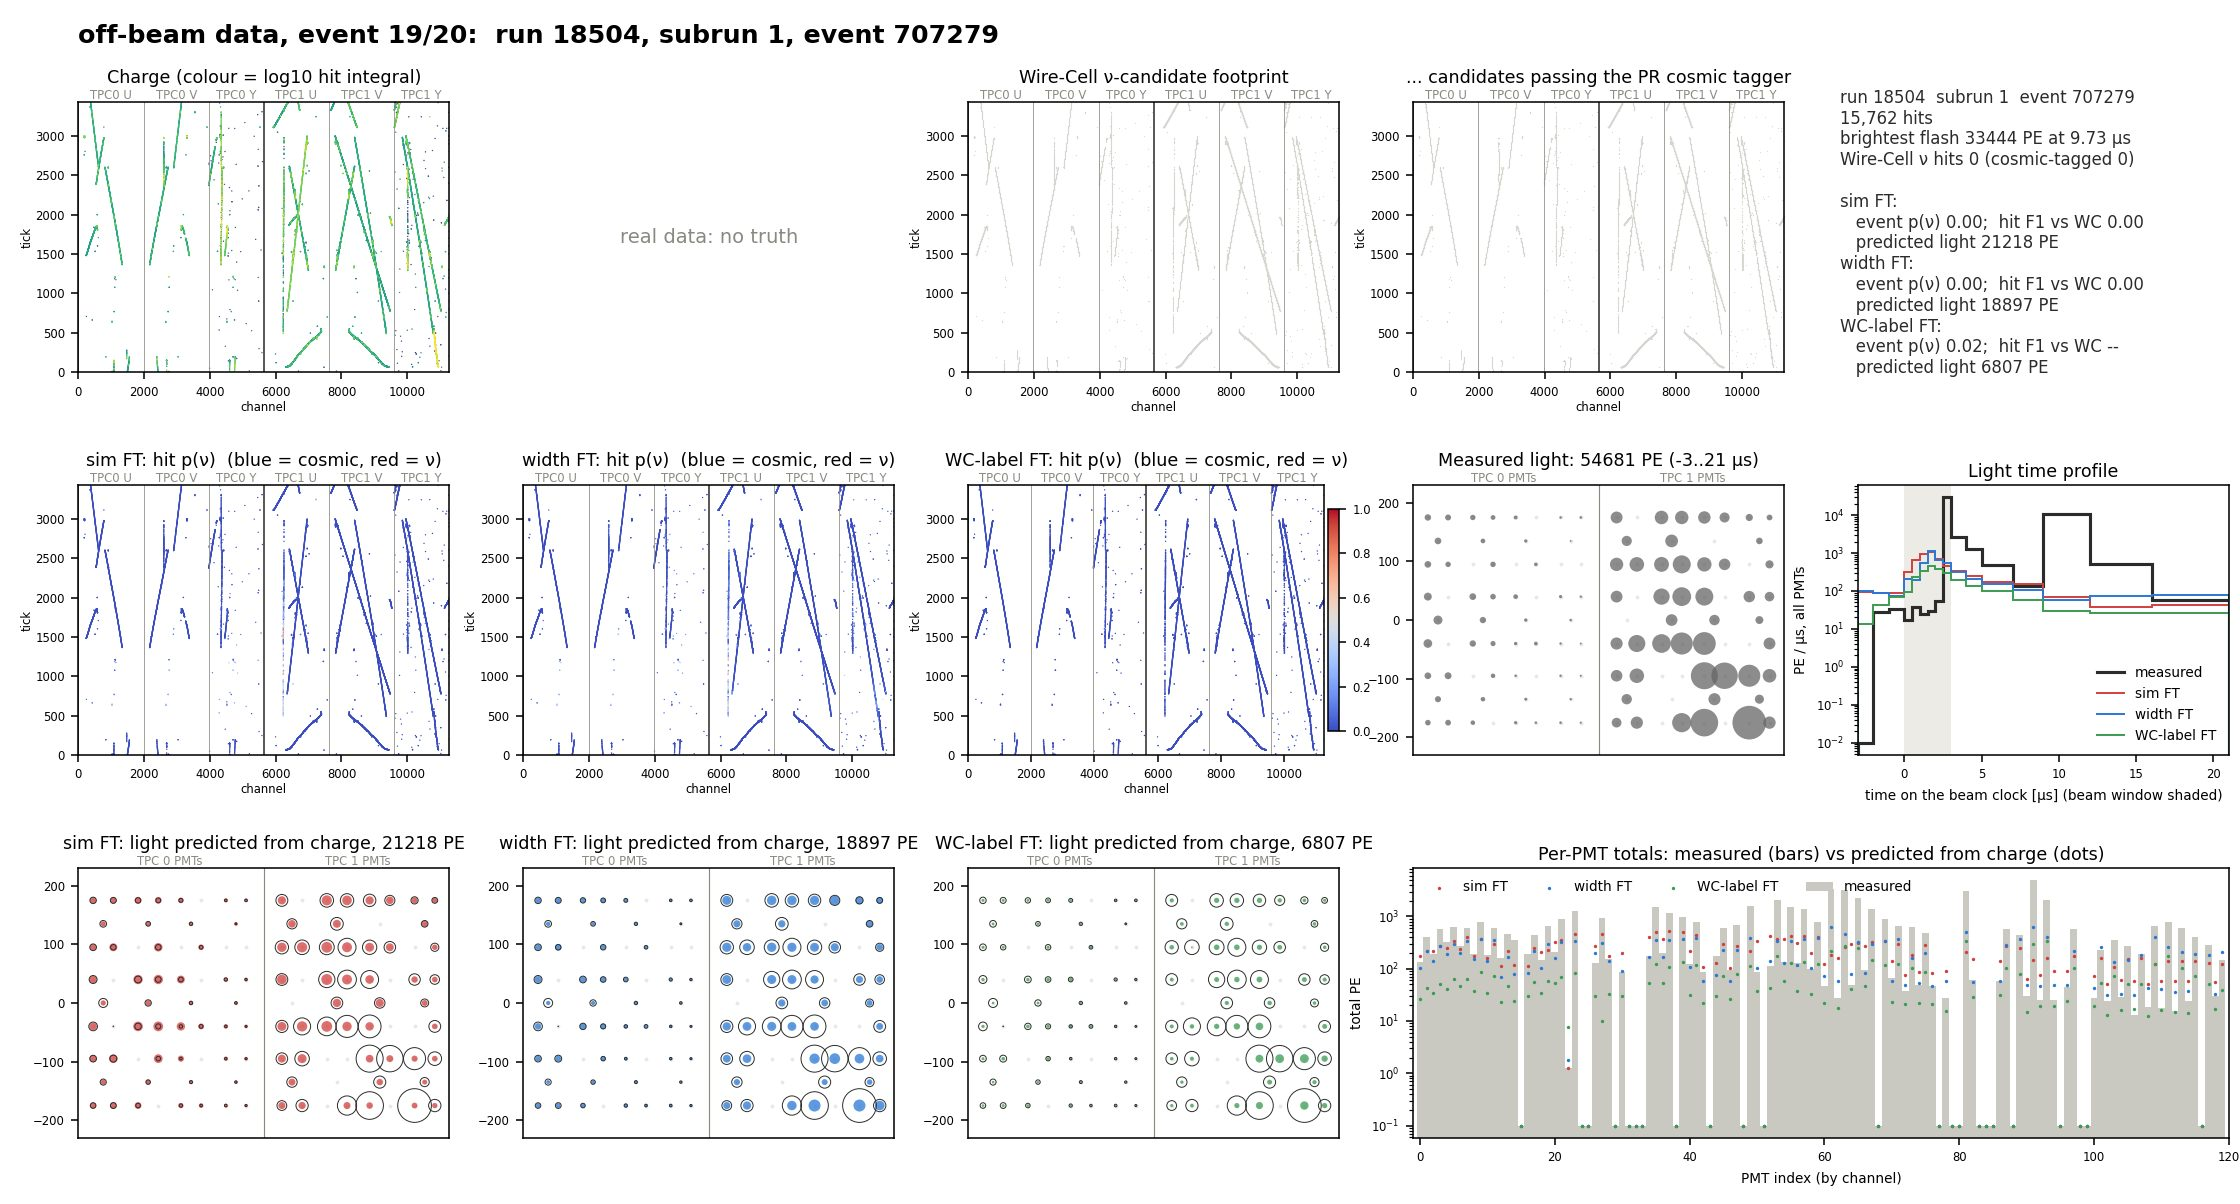
\includegraphics[width=\paperwidth,height=\paperheight,keepaspectratio]{displays/off_18.jpg}}
\end{frame}
% Off-beam data 20/20: run 18388, subrun 1, event 321351; event p(nu): sim FT 0.00, width FT 0.00, WC-label FT 0.04
\begin{frame}[plain]
  \centering\vspace*{-2pt}
  \makebox[\linewidth][c]{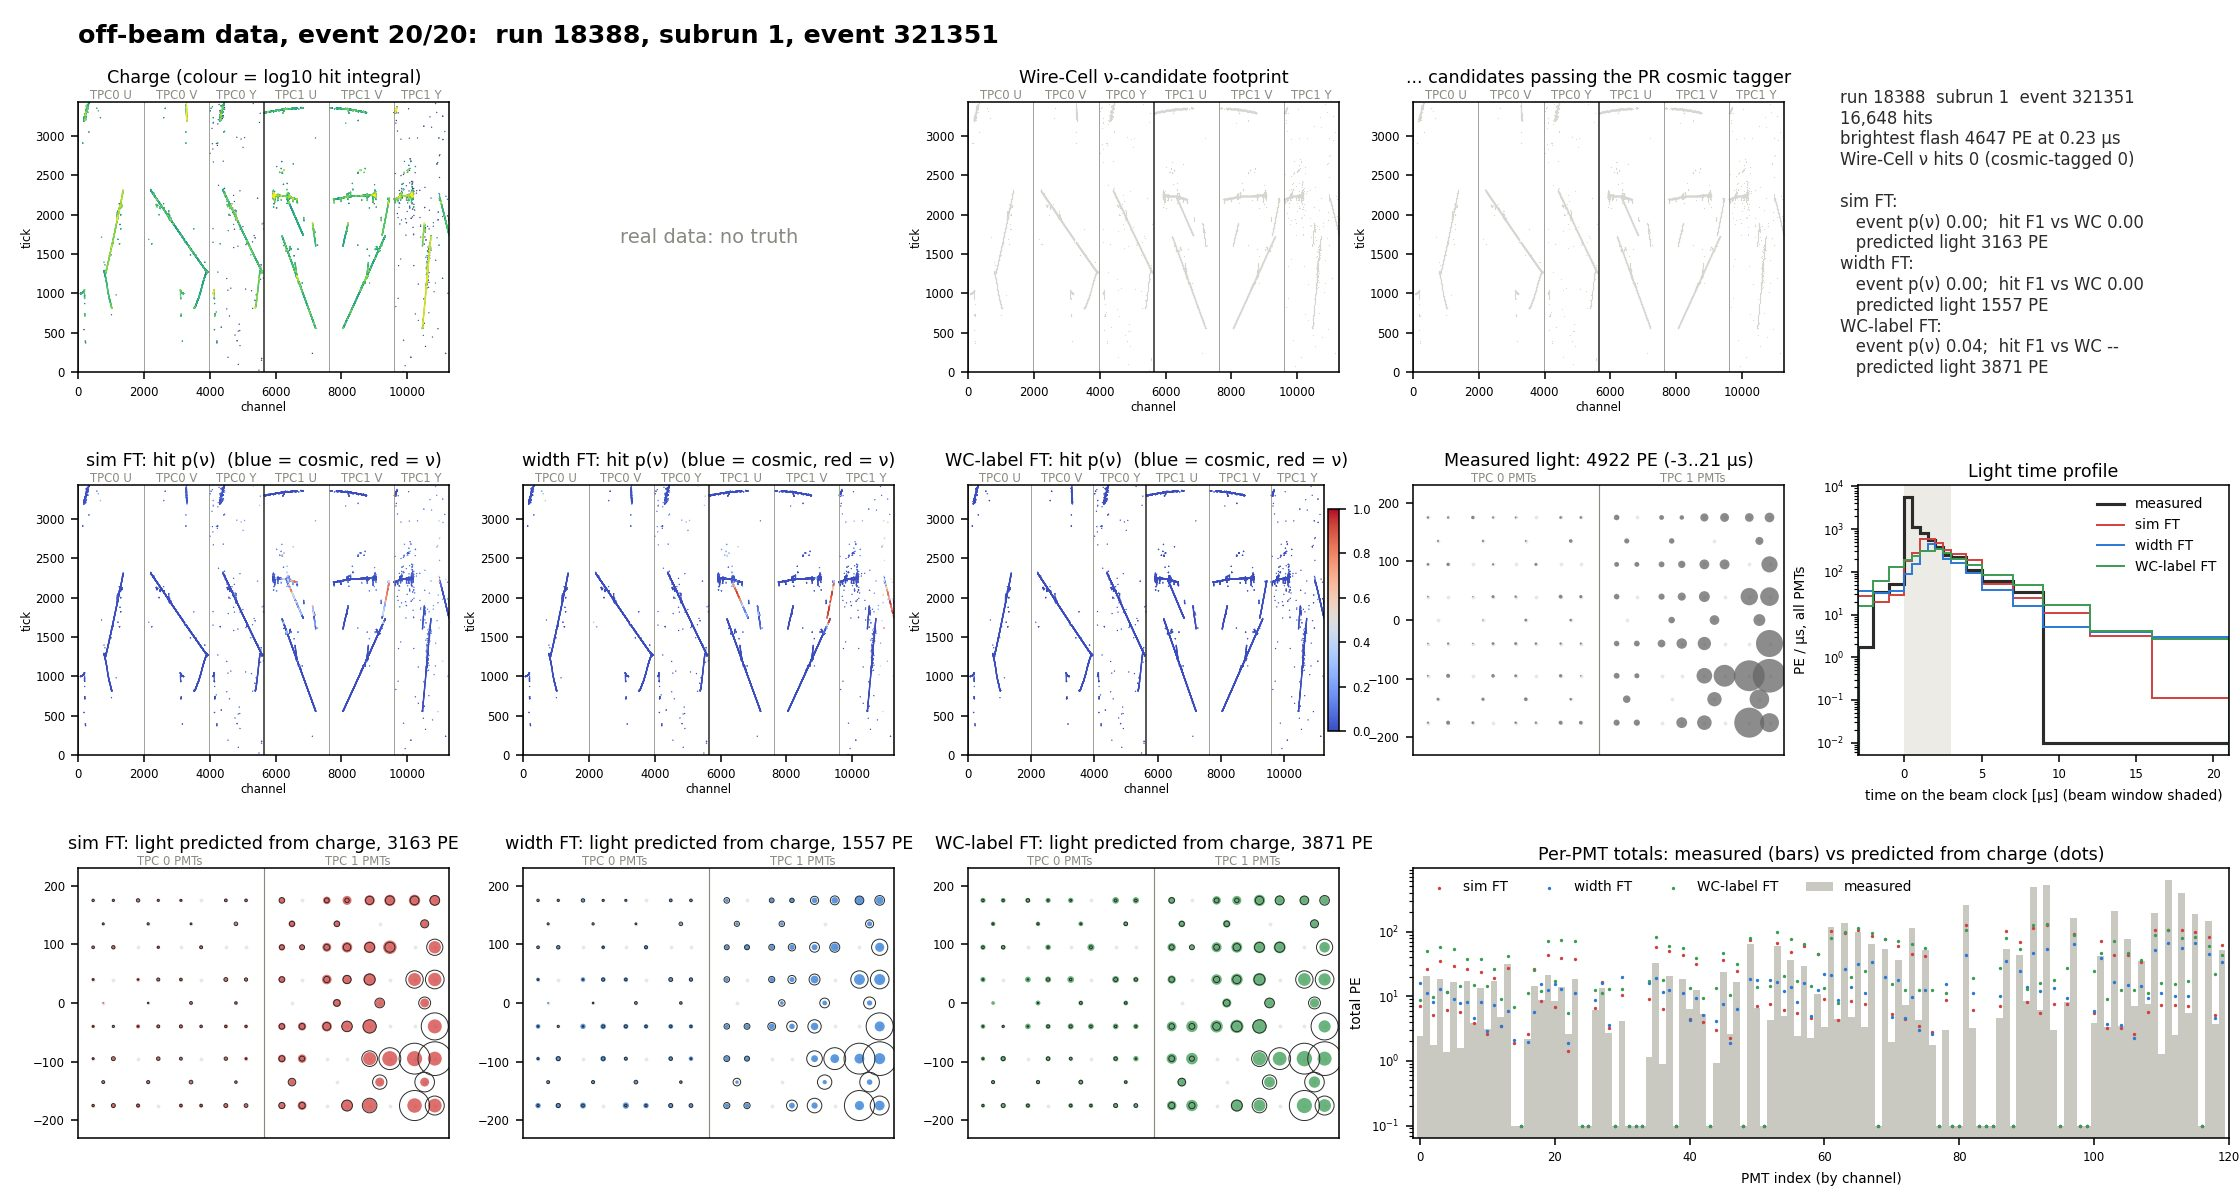
\includegraphics[width=\paperwidth,height=\paperheight,keepaspectratio]{displays/off_19.jpg}}
\end{frame}


%=====================================================================
\begin{frame}{Backup: where everything is}
  \scriptsize
  \begin{itemize}\setlength{\itemsep}{3pt}
    \item \textbf{Issue log:} \iss{14} (production, first look, E4, trigger note), \iss{11} (simulation samples, label fix).
    \item \textbf{Docs:} \doc{sbnd-realdata.md} (recipe, label definition), \doc{sbnd-h5maker.md} (simulation sample),
      \doc{data-inventory-sbnd.md}, \doc{experiments-live.pdf} (status board).
    \item \textbf{Data:} \code{fm4npp-lartpc-data/sbnd-data-\{bnb-opendata,offbeam-intime-run1\}/} (\code{full/}, \code{lists/}, README with POT and upstream selection).
    \item \textbf{Caches:} \code{\$QLFM\_WORK/cache/sbnd\_data\_m/} (data), \code{cache/sbnd\_m/} (simulation).
    \item \textbf{Results:} \code{\$QLFM\_WORK/sbnd\_data/firstlook.json}; \code{sbnd\_data/eval/<run>/report.json}, all runs in \code{report\_all.jsonl}.
    \item \textbf{Code} (fm4npp-lartpc main): converter data mode 5af5e9a; first look eb29862; \code{eval\_sbnd\_data} 548de25;
      \code{load\_run} fix 6987c12; E5--E7 options and display script 373f414; \code{sbnd-h5maker} 0.5 (\code{6d03818}), FermiGrid scripts (\code{c863a07}, \code{1f6c1a7}).
    \item \textbf{E5--E7 outputs:} \code{sbnd\_full/width/} (E6 models), \code{sbnd\_data/wcft/} (E7 models); evaluations in
      \code{sbnd\_data/eval/<run>/\{on,off,sim\_nom,sim\_w\}*}; event displays in \code{sbnd\_data/displays/} (\code{displays.json}).
    \item \textbf{Compute:} FermiGrid 37.5 CPU-h (production); Polaris about 4 node-h on \code{LArTPC\_FM} (conversion 0.03, E4 0.4,
      E5--E7 3.3, displays $<$0.1).
  \end{itemize}
\end{frame}

\end{document}
